\documentclass[11pt,fleqn]{article}
\linespread{1.3}
\usepackage{parskip}
\setlength{\parindent}{0pt} %no paragraph indentation
\setlength{\parskip}{2.1ex plus 0.2ex minus 0.2ex} %3x paragraph spacing
\usepackage{geometry}
\geometry{a4paper,left=30mm,right=25mm,top=20mm,bottom=20mm} %margin spacing
\usepackage{fancyhdr}
\pagestyle{fancy}
\fancyhf{}
\renewcommand{\headrulewidth}{0pt}
\rfoot{\thepage}

\usepackage[pdftex]{graphicx} %so that eps files may be included
\newcommand{\indep}{\rotatebox[origin=c]{90}{$\models$}} % so that \indep works :)
\usepackage[fleqn]{amsmath}
\usepackage{amssymb}
\usepackage{amsthm}
\usepackage{float}
\usepackage[bottom]{footmisc}

% Theorems, definitions etc.
\newtheoremstyle{defstyle}
  {10pt} % Space above
  {0pt} % Space below
  {} % Body font
  {} % Indent amount
  {\bfseries} % Theorem head font
  {.} % Punctuation after theorem head
  {0.5em} % Space after theorem head
  {} % Theorem head spec (can be left empty, meaning `normal')
\theoremstyle{defstyle}
\newtheorem{defn}{Definition}[section]
\newtheorem{rmrk}{Remark}[section]
\newtheorem{thrm}{Theorem}[section]
\newtheorem{ax}{Axiom}[section]

\usepackage{comment}

%\includeonly{./docs/linear_models,./docs/nonlinear_models,./docs/linear_control}
%\includeonly{./docs/linear_models,./docs/linear_control}
%\includeonly{./docs/lit_back,./docs/linear_control}
%\includeonly{./docs/linear_control}
%\includeonly{./docs/lit_back}

\begin{document}
\graphicspath{{./imgs/}{../imgs/}} %look for images

%Title page
\documentclass[../masters.tex]{subfiles}
\begin{titlepage}

\center % Center everything on the page
 
%----------------------------------------------------------------------------------------
%	HEADING SECTIONS
%----------------------------------------------------------------------------------------

\textsc{\LARGE University of Pretoria}\\[1.5cm] % Name of your university/college
\textsc{\Large Department of Chemical Engineering}\\[0.5cm] % Major heading such as course name
\textsc{\large Masters Dissertation}\\[3.5cm] % Minor heading such as course title

%----------------------------------------------------------------------------------------
%	TITLE SECTION
%----------------------------------------------------------------------------------------


\huge \textsc{Stochastic Dynamical Control using Graphical Models} \\[3.5cm]
 
%----------------------------------------------------------------------------------------
%	AUTHOR SECTION
%----------------------------------------------------------------------------------------

\begin{minipage}{0.4\textwidth}
\begin{flushleft} \large
\emph{Author:}\\
St. Elmo Wilken % Your name
\end{flushleft}
\end{minipage}
~
\begin{minipage}{0.4\textwidth}
\begin{flushright} \large
\emph{Student Number:} \\
29034133 
\end{flushright}
\end{minipage}\\[2cm]

\begin{minipage}{0.4\textwidth}
\begin{flushleft} \large
\emph{Co-Supervisor:}\\
Mr. C Sandrock % Your name
\end{flushleft}
\end{minipage}
~
\begin{minipage}{0.4\textwidth}
\begin{flushright} \large
\emph{Department:} \\
Chemical Engineering
\end{flushright}
\end{minipage}\\[2cm]

\begin{minipage}{0.4\textwidth}
\begin{flushleft} \large
\emph{Co-Supervisor:}\\
Dr. JP de Villiers % Your name
\end{flushleft}
\end{minipage}
~
\begin{minipage}{0.4\textwidth}
\begin{flushright} \large
\emph{Department:} \\
Electrical, Electronic and Computer Engineering
\end{flushright}
\end{minipage}\\ [2cm]

%----------------------------------------------------------------------------------------
%	DATE SECTION
%----------------------------------------------------------------------------------------

{\large \today}\\[3cm] % Date, change the \today to a set date if you want to be precise

\vfill % Fill the rest of the page with whitespace

\end{titlepage}
\tableofcontents
\chapter{Introduction}
This dissertation deals with the development of predictive controllers within the framework of probabilistic graphical models, specifically dynamic Bayesian networks. Dynamic Bayesian networks are well suited to the study of stochastic processes i.e. processes where there is noise in both the state evolution and state measurements. By leveraging the natural formulation of stochastic processes within dynamic Bayesian networks we develop stochastic predictive controllers, focusing specifically on linear quadratic Gaussian (LQG) and chance constrained model predictive control (MPC).

The dissertation primarily deals with the two graphical models\footnote{Clear circular nodes represent latent variables, shaded circular nodes represent observed variables and diamond nodes are deterministic variables.} shown in figures~\ref{fig_linear} and~\ref{fig_switch_linear}. Inference is discussed in general, but we focus on filtering and prediction because they are important for control. 
\begin{figure}[H]
 \centering
\begin{minipage}[b]{0.45\textwidth}
 \centering
\begin{tikzpicture}

  % Define nodes
  \node[obs] (ya) {$y_0$};
  \node[obs, right=of ya] (yb) {$y_1$};
  \node[obs, right=of yb] (yc) {$y_2$};
  \node[latent, above=of ya]  (xa) {$x_0$};
  \node[latent, above=of yb, right=of xa]  (xb) {$x_1$};
  \node[latent, above=of yc, right=of xb]  (xc) {$x_2$};
  \node[det, above=of xa] (da) {$u_0$};
  \node[det, above=of xb] (db) {$u_1$};
  
  % Connect the nodes
  \edge {da} {xb};
  \edge {db} {xc};
  \edge {xa} {ya};
  \edge {xb} {yb};
  \edge {xc} {yc};
  \edge {xa} {xb};
  \edge {xb} {xc};
  
\end{tikzpicture}
\caption{Single model probabilistic graphical model.}
\label{fig_linear}
\end{minipage}\hfill
\begin{minipage}[b]{0.45\textwidth}
 \centering
\begin{tikzpicture}

  % Define nodes
  \node[obs] (ya) {$y_0$};
  \node[obs, right=of ya] (yb) {$y_1$};
  \node[obs, right=of yb] (yc) {$y_2$};
  \node[latent, above=of ya]  (xa) {$x_0$};
  \node[latent, above=of yb, right=of xa]  (xb) {$x_1$};
  \node[latent, above=of yc, right=of xb]  (xc) {$x_2$};
  \node[det, above=of xa, xshift=0.7cm] (da) {$u_0$};
  \node[det, above=of xb, xshift=0.7cm] (db) {$u_1$};
  \node[latent, above=of xa, yshift=1.1cm] (sa) {$s_0$};
  \node[latent, above=of xb, yshift=1.1cm] (sb) {$s_1$};
  \node[latent, above=of xc, yshift=1.1cm] (sc) {$s_2$};
  
  % Connect the nodes
  \edge {da} {xb};
  \edge {db} {xc};
  \edge {xa} {ya};
  \edge {xb} {yb};
  \edge {xc} {yc};
  \edge {xa} {xb};
  \edge {xb} {xc};
  \edge {sa} {sb};
  \edge {sb} {sc};
  \edge {sa} {xa};
  \edge {sb} {xb};
  \edge {sc} {xc};
\end{tikzpicture}
\caption{Model switching probabilistic graphical model.}
\label{fig_switch_linear}
\end{minipage}
\end{figure}
The dissertation is structured in 3 parts, each composed of self contained chapters dealing with a specific problem area. Part \ref{part_one} contains chapters \ref{sec_lit_study} to \ref{sec_cstr}. The literature review, chapter \ref{sec_lit_study}, deals with current papers on topics related to this dissertation. Chapter \ref{sec_back_theory} mainly deals with background theory found in reference materials (e.g. books). Chapter \ref{sec_hmm} deals with hidden Markov models. The goal of this chapter is to gently introduce the uninformed reader to the power of graphical models. Finally, chapter \ref{sec_cstr} introduces the continuously stirred tank reactor (CSTR) example which is used to illustrate the techniques investigated throughout the rest of the dissertation. If the reader is familiar with graphical models, predictive control and CSTR design part \ref{part_one} may be safely skipped.

Parts \ref{part_two} and \ref{part_three} each follow the same pattern: a graphical model is introduced and studied after which a control scheme is implemented using the tenets of the preceding work. We detail the content and results of these two parts next.

In part \ref{part_two} the dynamic Bayesian network, shown in figure \ref{fig_linear}, is investigated within the context of the Kalman filter model (linear dynamics and Gaussian noise) and the particle filter model (no assumptions about the dynamics and noise). Using the techniques endemic to the aforementioned probabilistic graphical models we show:
\begin{enumerate}
\item
That the LQG controller reduces to the linear quadratic regulator under the assumptions of normality and linearity \footnote{This result is not new but the derivation using probabilistic graphical models is both instructive and, more importantly, intuitive.}.
\item
That a chance constrained MPC problem can be reduced to the standard form MPC problem (a deterministic optimisation problem with linear constraints and a quadratic objective function) under the assumptions of linearity and normality. Furthermore, since the Mahalanobis distance, a statistically important measure, is used to reduce the chance constraints to linear constraints it supports the application of the aforementioned techniques to systems which are nonlinear and non-Gaussian. 
\end{enumerate}
In part~\ref{part_three} the switching model filter, based on the dynamic Bayesian network shown in figure~\ref{fig_switch_linear}, is investigated\footnote{This probabilistic graphical model uses a set of models to perform inference. The stochastic switching variables $(s_0, s_1,...)$ are used to weight the likelihood of each model supporting the observations.}. The benefit of generalising figure~\ref{fig_linear} is that it allows one to infer which model, from a set of possible models, is likely to be generating the observations. This allows us to extend the stochastic MPC discussed previously to incorporate model switching. We investigate the following:
\begin{enumerate}
\item
Using the Rao-Blackwellised particle filter as the switching model filter. In this context the resultant most likely linear model is used to move the underlying system to different regions in state space. It was found that the approach caused controller instability because the current most likely model is often not accurate enough to steer the system to the target.
\item
Using a switching particle filter as the switching model filter. In this context the filter was used to identify when a process fault occurred and, based on this event, switch the model control is based upon. It was found that the algorithm successfully stabilised and regulated the nonlinear underlying system.
\end{enumerate}
Perhaps most usefully, the dissertation illustrates the advantage of designing model predictive controllers from within the framework of probabilistic graphical models. While it may seem that the two fields are not related, most modern control systems perform filtering on system measurements which is a natural result of the application of probabilistic graphical models. Therefore, the motivation for this study is not purely esoteric but demonstrates a tacit relationship between the fields.   

\textbf{A note on implementation:}\\
Although this dissertation spends much time investigating and developing theory there is also a significant practical aspect. All the results are supported by robust simulations. The Julia language \cite{julia} was used to implement and illustrate the effectiveness of the succeeding algorithms. Both the Ipopt \cite{ipopt} and Mosek \cite{mosek} optimisation libraries were used in conjunction with Julia's optimisation modelling package JuMP \cite{jump}. Matplotlib \cite{pyplot} was used to plot the results. All the code used in this dissertation is available on Github at \url{https://github.com/stelmo/Stochastic-Dynamical-Control-Code}.
\section{Background Literature}
This section is composed of five subsections which introduce the main concepts and results used throughout the rest of the document. Section \ref{sec_prob_theory} introduces Probability Theory. Section \ref{sec_graph_theory} very briefly introduces some useful nomenclature from Graph Theory. These two sections serve as an entry point for Section \ref{sec_graphical_models_theory} which deals with Probabilistic Graphical Models. Section \ref{sec_lit_control} deals with Control Theory and Section \ref{sec_block} introduces an important result from matrix linear algebra.

It would seem as if Sections \ref{sec_prob_theory} to \ref{sec_graphical_models_theory} and Section \ref{sec_lit_control} are not related to each other. However, the foundational theory introduced here is expanded upon later and the relationship then becomes clear.

\subsection{Probability Theory}
\label{sec_prob_theory}
The calculus of Probability Theory was developed by Fermat and Pascal in order to better understand the problems introduced by uncertainty in gambling. From this dubious genesis a rich and incredibly powerful field has developed. We start our brief introduction of probability theory by restating Kolmogorov's three probability axioms - these axioms underpin the entire theory of probability.

Let the set $\Omega$ be the universe of possible events, also called the event space; that is, if we are uncertain about which of a number of possibilities are true then we let $\Omega$ represent all of them collectively. Let $P$ be some real valued function which satisfies the three axioms stated below.
\begin{ax}
$P(\Omega) = 1$. The probability of any event in $\Omega$ occurring is 1.
\end{ax}
\begin{ax}
$\forall \alpha \in \Omega,~P(\alpha) \geq 0$. The probability of any one (or set of) event(s) in $\Omega$ occurring is non-negative. 
\end{ax}
\begin{ax}
$\forall \alpha, \beta \in \Omega,\text{ if } \alpha \cap \beta = \emptyset \text{ then } P(\alpha \cup \beta) = P(\alpha) + P(\beta)$. The probability of two mutually disjoint sets of events in $\Omega$ occurring is equal to the sum of their probabilities.
\end{ax}
A function $P$ which satisfies these three axioms is known as a probability function. Based on these three axioms we are able to extend the theory to Theorem \ref{thrm_prob_union_intersect}.
\begin{thrm}
$\forall \alpha, \beta \in \Omega, P(\alpha \cup \beta) = P(\alpha) + P(\beta) + P(\alpha \cap \beta)$. The probability of two events occurring in $\Omega$ is equal to the sum of their probabilities less the probability of both occurring simultaneously.
\label{thrm_prob_union_intersect}
\end{thrm}

\subsubsection{Discrete Random Variables}

We now make precise what we mean by random variables: a random variable is a non-deterministic variable which is characterised by some uncertainty in its measurement. Semantically we indicate a specific value taken on by the random variable $X$ as $X=x$ or just denote it $x$. Thus, the function $P(X=x)=P(x) \in \mathbb{R}$ indicates the probability of event $x$ occurring with respect to the random variable $X$. We denote $P(X)$ as the probability function of the random variable $X$. Thus, for the discrete random variable $X$ we have that $P(X)=(P(x_1),P(x_2),...,P(x_n))^T$ where $x_i \in X$ for $i=1,2,..., n$ and $\sum_i P(x_i) =1$. We defer the study of the continuous case until later.

Before we proceed let us briefly discuss how we can interpret the function $P$ for any random variable $X$. If $P(X=x)=1$ we are certain of event $x$ occurring, i.e. $X$ will only take on the value $x$. If $P(x)=0$ we are certain that event $x$ will not occur, i.e. $X$ will never take on the value $x$. Thus our certainty of event $x$ occurring is reflected by the magnitude of $P(x)$. Attempting to make the statement ``our certainty of event $x$ occurring" more precise leads us to two different physical interpretations of $P(x)$. The first is the frequentist interpretation: to the frequentist a probability is a long term average of the observations of event $x$ occurring in the event space. While this interpretation is satisfying if one deals with something which is easily measured e.g. the probability of a fair die rolling a 6, it fails to explain statements like: ``the probability of it raining tomorrow is 50\%". The reason the last statement is problematic is because the time span is ill defined. If we rather understand probabilities to mean subjective degrees of belief in event $x$ occurring this is no longer a problem. To ensure that these subjective beliefs are rational can be problematic. One way to ensure this is by requiring that if the probabilities were used in a betting game it is impossible to exploit them to one's advantage (or disadvantage). If this is possible then there is no difference between the interpretations described above \cite{koller}. 

We will deal extensively with joint and marginal probability distributions. Consider the random variables $X$ and $Y$. The marginal probability distribution of $X$ is the function $P(X)$ and describes the probabilities of events involving only the variable $X$. The joint probability distribution of $X$ and $Y$ is the function $P(X,Y) = P(X \cap Y)$ and describes the intersection (and) of the probability space of $X$ and $Y$. We introduce, without proof, Theorem \ref{thrm_marg}.
\begin{thrm}
\textbf{Marginalisation} By marginalising out $X$ we mean we sum out $X$ from the joint distribution $P(Y) = \sum_x P(x, Y)$. This extends to higher dimensions. 
\label{thrm_marg}
\end{thrm}
We can reduce any joint distribution to a marginal one by summing (or integrating in the case of continuous random variables) out the appropriate variable. 

It is now necessary to define what we mean by conditional probability. Definition \ref{defn_cond_prob} makes precise how the knowledge that event $y$ has occurred alters our view of event $x$ occurring.  
\begin{defn}
\textbf{Conditional Probability} $P(X|Y) = \frac{P(X \cap Y)}{P(Y)}$ 
\label{defn_cond_prob}
\end{defn}
Note that if for some $y \in Y$ we have $P(Y=y) = 0$ then Definition \ref{defn_cond_prob} is undefined. Additionally, the function $P(\cdot|Y)$ is a probability function. We next define what we mean by a positive probability distribution in Definition \ref{defn_pos_distr}.
\begin{defn}
A probability distribution is positive if $P(x) > 0~\forall~x \in X$.
\label{defn_pos_distr}
\end{defn}
Clearly undefined conditional probabilities are not a problem in the setting of positive probability distributions. We also define the notion of independence, also sometimes called marginal independence, in Definition \ref{defn_indep}. 

As before, let $X$, $Y$ and $Z$ be random variables. Intuitively $X$ and $Y$ are independent if the outcome of $X$ does not influence the outcome of $Y$. It can be shown that independence is a symmetric property \cite{koller}.
\begin{defn}
\textbf{Independence} $X \indep Y \equiv P(X|Y) = P(X)$ 
\label{defn_indep}
\end{defn}
Generalising the concept of independence we define conditional independence by Definition \ref{defn_cond_indep}. Again this definition is symmetric \cite{koller}.
\begin{defn}
\textbf{Conditional Independence} $X \indep Y | Z \equiv P(X|Y,Z) = P(X|Z)$
\label{defn_cond_indep}
\end{defn}
Intuitively, if $X$ is conditionally independent of $Y$ given $Z$ then by observing $Z$ one gains nothing by observing $Y$. Clearly if $Z=\emptyset$ we have (marginal) independence. We also introduce Theorem \ref{thrm_chain_rule} which naturally leads us to the formulation of Bayes' Theorem (using Definition \ref{defn_cond_prob}) as shown in Theorem \ref{thrm_bayes}. 
\begin{thrm}
\label{thrm_chain_rule}  
\textbf{Chain Rule} Given the random variables $X_1$ and $X_2$ we have $P(X_1,X_2) = P(X_1)P(X_2|X_1)$. The generalisation to an arbitrary number of random variables is straightforward.
\end{thrm}
\begin{thrm}
\textbf{Bayes' Theorem} $P(X|Y) = \frac{P(Y|X)P(X)}{P(Y)}$
\label{thrm_bayes}
\end{thrm}
Under the Bayesian interpretation of Theorem \ref{thrm_bayes} we see that the posterior probability of some hypothesis $X$ given some evidence $Y$ being true is just the likelihood $P(Y|X)$ of the hypothesis supporting the evidence multiplied by the prior probability of the hypothesis $P(X)$ normalised by the prior of the evidence $P(Y)$. It is also convenient to notice that $P(Y)$ is a normalising constant and thus  $P(X|Y) \propto P(Y|X)P(X)$.

To fully describe a system of random variables it is only necessary to know the joint distribution $P(X_1,X_2,...,X_n)$. Given the joint probability distribution inference (reasoning about the variables under uncertainty) may be performed. Common probabilistic queries involve computing posterior beliefs $P(X|Y=y)$ i.e. the probability function of $X$ given we have some information about $Y$. Other queries involve find the most probable explanation (called a MAP query) of some evidence i.e. finding $X$ which maximises $P(X, Y=y)$. More on this later. 

\textbf{Bayes' Theorem: Example}\\
This section will attempt to develop some intuition behind Theorem \ref{thrm_bayes}. We quote an excerpt from an article in the Economist \cite{eco1} and illustrate the use of Bayes' Rule in a canonical medical example \cite{korb}.

\textit{``The essence of the Bayesian approach is to provide a mathematical rule explaining how you should change your existing beliefs in the light of new evidence. In other words, it allows scientists to combine new data with their existing knowledge or expertise. The canonical example is to imagine that a precocious newborn observes his first sunset, and wonders whether the sun will rise again or not. He assigns equal prior probabilities to both possible outcomes, and represents this by placing one white and one black marble into a bag. The following day, when the sun rises, the child places another white marble in the bag. The probability that a marble plucked randomly from the bag will be white (ie, the child's degree of belief in future sunrises) has thus gone from a half to two-thirds. After sunrise the next day, the child adds another white marble, and the probability (and thus the degree of belief) goes from two-thirds to three-quarters. And so on. Gradually, the initial belief that the sun is just as likely as not to rise each morning is modified to become a near-certainty that the sun will always rise."}

Suppose you get tested for a certain disease. You know the disease affects 1 in 100 people. You also know that the false positive rate for the test is 20\% and the false negative rate for the test is is 10\%. Your test comes back positive. What are the chances of you having the disease given this information?

The information may be summarised as shown below. Let $D$ be a binary random variable indicating the presence of the disease and $\neg D$ indicates the absence. Let $T$ be a binary random variable indicating a positive test and $\neg T$ indicates a negative test. 
\begin{enumerate}
\item
The prior of the disease is $P(D) = 0.01$.
\item
False positive rate $P(T|\neg D) = 0.2 \implies P(\neg T|\neg D) = 0.8$.
\item
False negative rate $P(\neg T|D) = 0.1 \implies P(T|D) = 0.9$.
\end{enumerate}
A naive approach would conclude that since $P(T|D) = 0.9$ you are 90\% likely to have the disease. However, using Bayesian inference/reasoning we have: 
\begin{equation*}
\begin{aligned}
P(D|T) &= \frac{P(T|D)P(D)}{P(T)} \\
&=  \frac{P(T|D)P(D)}{\sum_D P(D,T)} \\
&= \frac{P(T|D)P(D)}{\sum_D P(D)P(T|D)} \\
& = \frac{0.9 \times 0.01}{0.01 \times 0.99 + 0.99 \times 0.2} \\
&\approx 0.04
\end{aligned}
\end{equation*}
Clearly there is a big difference between the naive approach and the Bayesian (correct) approach. The power of Bayesian inference lies in the ability to reverse causal reasoning. That is, we know that the disease causes the test to be positive, $P(T|D)$, but we would like to reverse this reasoning to infer $P(D|T)$. This is immensely powerful as we shall soon discover.   

\subsubsection{Continuous Random Variables}

So far in our discussion we have implicitly only used discrete random variables; that is, our probability space consisted out of a finite number of events or states. However, it is also necessary to make precise what we mean by a continuous random variable. A continuous random variable is characterised by a density function $p$ which assigns a weight to each possible value of the variable. Intuitively this weight is \underline{related} to the probability of that value occurring\footnote{Please note that strictly speaking $P(x)=0$ for a specific point $x$ in the domain of $p$. Technically it is correct to say that the probability of $P(x \in [a,b]) = \int_a^b p(y)dy$; thus, if we want the probability of $x$ occurring we could just make $[a,b]$ small.}. Although the density function is itself not a probability function, if it satisfies $p(x) \geq 0~\forall x \in X$ and $\int p(x)dx = 1$, where we have implicitly integrated over the domain of $p$, then it can be used to generate one. The cumulative probability function $P(X \leq a)=\int^a_{-\infty} p(x)dx$ is one such example\footnote{We have assumed that the domain of $X$ is the entire real line.}. 

Arguably the most well known continuous probability density distribution is the Gaussian or Normal distribution. The Gaussian distribution arises naturally from a variety of different contexts and settings. For example, the central limit theorem, together with some mild assumptions, tells us that the sum of a set of $N$ random  variables is itself a random variable and in the limit can be described by a Gaussian distribution \cite{bishop}. The Gaussian is regularly used because it has some very appealing analytical properties (and also often because it is physically meaningful) which we will investigate in some depth. 

Since the probability of a specific value is not meaningful in the setting of continuous probability functions we abuse our notation and interchangeably denote the random variable $X$ by $x$. We also do not indicate vector quantities in boldface; it can be assumed that all numbers are vectors unless otherwise noted. We will concern ourselves mostly with vector quantities and it will be obvious when we deal with non-vector valued variables. 
\begin{defn}
\textbf{Gaussian Distribution} The univariate Gaussian or Normal distribution of a random variable $x$ is shown in (\ref{eq_norm_uni}). We call $\mu$ the mean and $\sigma^2$ the variance of the distribution.
\begin{equation}
\mathcal{N}(x|\mu, \sigma^2) = \frac{1}{\sqrt{2\pi\sigma^2}}\exp\left(-\frac{1}{2\sigma^2}(x-\mu)^2\right)
\label{eq_norm_uni}
\end{equation}
The multivariate Gaussian distribution is shown in (\ref{eq_norm_multi}) where $\mu$ is a $D$ dimensional mean vector and $\Sigma$ is a $D \times D$ dimensional covariance matrix. Note that we often use the inverse of the covariance matrix, called the precision matrix and define it $\Lambda \equiv \Sigma^{-1}$.
\begin{equation}
\mathcal{N}(x|\mu, \Sigma) = \frac{1}{\sqrt{2\pi^{\frac{D}{2}}}}\frac{1}{|\Sigma|^{\frac{1}{2}}}\exp\left(-\frac{1}{2}(x-\mu)^T\Sigma^{-1}(x-\mu)\right)
\label{eq_norm_multi}
\end{equation}
\label{defn_gauss}
\end{defn}
It is also appropriate to define some functions which apply equally well to the discrete case as to the continuous case (just replace the integration with summation in the setting of discrete random variables). We define the expectation (or mean or average) in Definition \ref{def_expectation}, the variance in Definition \ref{def_variance} and the covariance in Definition \ref{def_covariance}. 
\begin{defn}
\textbf{Expectation} The average value of some integrable function $f$ under the probability distribution $p$ is denoted $\mathbb{E}[f] = \int p(x)f(x)dx$.
\label{def_expectation}
\end{defn}
We have that $\mathbb{E}[x]=\mu$ if $x$ is a Gaussian random variable.
\begin{defn}
\textbf{Variance} The variance of $f$ is defined by $\text{var}[f] = \mathbb{E}[(f - \mathbb{E}[f])^2]$ and provides a measure of how much variability there is in $f$ around its mean value $\mathbb{E}[f]$.
\label{def_variance}
\end{defn}
By expanding out the square we have the familiar formulate $\text{var}[f] = \mathbb{E}[f^2] - \mathbb{E}[f]^2$. Also note that for a  univariate Gaussian random variable $x$ we have $\text{var}[x] =\sigma^2$.
\begin{defn}
\textbf{Covariance} For two random variables $x,y$ (which may be vectors) we define the covariance matrix $\text{cov}[x,y] = \mathbb{E}[xy^T] - \mathbb{E}[x]\mathbb{E}[y]$.
\label{def_covariance}
\end{defn}
Note that $\text{cov}[x,x]=\text{cov}[x]=\text{var}[x]$. Covariance is a measure of how much two random variables vary together. If $x$ is a $D$ dimensional Gaussian random variable then $\text{cov}[x] = \Sigma$ as defined in Definition \ref{defn_gauss}.

The identities in Theorem \ref{thrm_gaussian_identities} will be useful in later sections. We refer the reader to \cite{davidian} for justification.
\begin{thrm}
\textbf{Gaussian Expected Value Identities}
Suppose there exist constants $c \in \mathbb{R}^n$ and $C \in \mathbb{R}^{n \times n}$ and $X$ is a normal random variable with statistics $(\mu, \Sigma)$. Then the following identities hold:
\begin{enumerate}
\item
$\mathbb{E}[c^TX] = c^T\mu$
\item
$\mathbb{E}[CX+c] = C\mu + c$
\item
$\mathbb{E}[X^TCX] = \text{tr}(C\Sigma) + \mu^TC\mu$
\end{enumerate}
\label{thrm_gaussian_identities}
\end{thrm}  

Now we are in a position to perform some manipulations assuming we are using Gaussian random variables. We state without proof Theorem \ref{thrm_joint_gaussians}.
\begin{thrm}
\textbf{Partitioned Joint Gaussians}
Given a Gaussian distribution $\mathcal{N}(x|\mu,\Sigma)$ with $\Lambda \equiv \Sigma^{-1}$ and $x=\begin{pmatrix}
x_a \\ x_b
\end{pmatrix}$, $\mu=\begin{pmatrix}
\mu_a \\ \mu_b
\end{pmatrix}$, $\Sigma=\begin{pmatrix}
\Sigma_{aa} & \Sigma_{ab} \\ \Sigma_{ba} & \Sigma_{bb}
\end{pmatrix}$ and $\lambda = \begin{pmatrix}
\Lambda_{aa} & \Lambda_{ab} \\ \Lambda_{ba} & \Lambda_{bb}
\end{pmatrix}$ then we have the conditional distribution in (\ref{eq_part_joint_gauss1}) and the marginal distribution in (\ref{eq_part_joint_gauss2}).
\begin{equation}
\begin{aligned}
&p(x_a|x_b) = \mathcal{N}(x_a|\mu_{a|b}, \Lambda_{aa}^{-1}) \\
&\text{with } \mu_{a|b} = \mu_a - \Lambda_{aa}^{-1}\Lambda_{ab}(x_b-\mu_b)
\end{aligned}
\label{eq_part_joint_gauss1}
\end{equation}
\begin{equation}
p(x_a) = \mathcal{N}(x_a|\mu_a,\Sigma_{aa})
\label{eq_part_joint_gauss2}
\end{equation}
\label{thrm_joint_gaussians}
Note that for the conditional distribution it is easier to work with the precision matrix. 
\end{thrm}
Next we state and then prove Theorem \ref{thrm_bayes_gaussians} which we will use extensively. The proof for Theorem \ref{thrm_joint_gaussians} uses the same techniques and can be found in \cite{bishop}.
\begin{thrm}
\textbf{Bayes' Theorem for Linear Gaussian Models}
Suppose we have a marginal Gaussian distribution for $x$ and a conditional Gaussian distribution for $y$ in the form shown in (\ref{eq_bayes_gauss_suppose}).
\begin{equation}
\begin{aligned}
p(x) &= \mathcal{N}(x|\mu,\Lambda^{-1}) \\
p(y|x) &= \mathcal{N}(y|Ax + b, L^{-1}) 
\end{aligned}
\label{eq_bayes_gauss_suppose}
\end{equation} 
Then the marginal distribution for $y$ is given by (\ref{eq_bayes_gauss1}) and the conditional distribution for $x$ given $y$ is (\ref{eq_bayes_gauss2}).
\begin{equation}
p(y) = \mathcal{N}(y|A\mu + b, L^{-1}+A\Lambda^{-1}A^T)
\label{eq_bayes_gauss1}
\end{equation}
\begin{equation}
\begin{aligned}
&p(x|y) = \mathcal{N}(x|\Sigma(A^TL(y-b)+\Lambda\mu), \Sigma) \\
&\text{with } \Sigma = (\Lambda + A^TLA)^{-1}
\end{aligned}
\label{eq_bayes_gauss2}
\end{equation}
\label{thrm_bayes_gaussians}
Note that $b$ is a known vector. Given a deterministic function $u$ we can also write $b = Bu + e$ where $B$ is some conforming matrix and $e$ is some constant vector. 
\label{thrm_bayes_lin_gauss_mod}
\end{thrm}
\begin{proof}
We begin our proof by noticing that for a general Gaussian $\mathcal{N}(\gamma|\alpha, \beta)$ we can write the exponent as in (\ref{eq_bg1}), note $const$ is some real number which does not depend on $\gamma$.
\begin{equation}
-\frac{1}{2}\left(\gamma-\alpha \right)^T\beta^{-1}\left(\gamma-\alpha \right) = -\frac{1}{2}\gamma^T\beta^{-1}\gamma +\gamma^T\beta^{-1}\alpha + const
\label{eq_bg1} 
\end{equation}
Also note that Gaussian distributions are closed under multiplication, i.e. if one multiplies two Gaussian distributions the product is still a Gaussian distribution (of a higher dimension). To find the joint distribution we let $z = \begin{pmatrix}
x \\ y
\end{pmatrix}$ and consider the log of the joint in (\ref{eq_log_gauss_joint}).
\begin{equation}
\begin{aligned}
\log(z) &= \log(p(x)) + \log(p(y|x))\\
&=  -\frac{1}{2}(x-\mu)^T\Lambda(x-\mu) -\frac{1}{2}(y-Ax-b)^T L(y-Ax-b) + const
\end{aligned}
\label{eq_log_gauss_joint}
\end{equation}
Here $const$ denotes constant terms which are independent of $x$ and $y$. Now we make use of (\ref{eq_bg1}) to find the mean and covariance of $z$. Continuing, we consider only the second order terms when (\ref{eq_log_gauss_joint}) is expanded, as shown in (\ref{eq_gauss_joint_precision}).
\begin{equation}
\begin{aligned}
&-\frac{1}{2}x^T(\Lambda+A^TLA)x-\frac{1}{2}y^TLy + \frac{1}{2}y^TLAx+\frac{1}{2}x^TA^TLy \\
&= -\frac{1}{2}\begin{pmatrix}
x \\ y
\end{pmatrix}^T \begin{pmatrix}
\Lambda+A^TLA & -A^TL \\ -LA & L
\end{pmatrix}\begin{pmatrix}
x \\ y
\end{pmatrix} \\
&= -\frac{1}{2}z^TRz
\end{aligned}
\label{eq_gauss_joint_precision}
\end{equation}
From this we immediately have the precision of $z$: the matrix $R$; we also use a matrix inversion formula found in \cite{bishop} to find the covariance. This is shown in (\ref{eq_gauss_covar}).
\begin{equation}
\text{cov}[z] = R^{-1} = \begin{pmatrix}
\Lambda^{-1} & \Lambda^{-1}A^T \\ A\Lambda^{-1} & L^{-1}+A\Lambda^{-1}A^T
\end{pmatrix}
\label{eq_gauss_covar}
\end{equation}
We now proceed in exactly the same way to find mean of $z$. By expanding \ref{eq_log_gauss_joint} and only considering the first order terms in $x$ and $y$ we have (\ref{eq_gauss_mean1}).
\begin{equation}
x^T\Lambda\mu-x^TA^TLb+y^TLb = \begin{pmatrix}
x \\ y
\end{pmatrix}\begin{pmatrix}
\Lambda\mu - A^TLb \\Lb
\end{pmatrix}
\label{eq_gauss_mean1}
\end{equation}
Again, by making use of (\ref{eq_bg1}) and the fact that the covariance of $z$ is $R^{-1}$ it is possible to show that $\mathbb{E}[z]=\begin{pmatrix}
\mu \\ A\mu +b
\end{pmatrix}$ as shown in \cite{bishop}. By using Theorem \ref{thrm_joint_gaussians} we immediately have the marginal and conditional distributions as required.
\end{proof}
We also introduce a useful metric for measuring the similarity between two distributions in Definition \ref{def_kl}. 
\begin{defn}
\textbf{Kullback-Leibler Divergence} Consider some unknown distribution $p(x)$ and suppose we have modelled this distribution by $q(x)$. Kullback-Leibler Divergence, also known as relative entropy, is defined $\text{KL}(p||q) = -\int p(x)\text{ln}\left(\frac{q(x)}{p(x)}\right)dx$ and measures the additional amount of information, in \textit{nats}, needed to specify the value of $x$ \cite{bishop}. 
\label{def_kl}
\end{defn}
Kullback-Leibler Divergence can be used to measure the dissimilarity between two distributions. If the measure is zero the distributions are identical; care needs to be taken when using Kullback-Leibler Divergence because the measure is not symmetric. We introduce Theorem to measure the dissimilarity between a known distribution and a sampled approximation thereof. See \cite{bishop} for the motivation.
\begin{thrm}
Suppose we observe a finite set of points $x_n$ for $n=1,2,..., N$ drawn from $p(x)$. Furthermore, suppose we would like to measure the information loss when $p$ is approximated by $q$. We can measure this by $\text{KL}(p||q) \approx \frac{1}{N}\sum_{n=1}^N\left(-\text{ln}(q(x_n)) + \text{ln}(p(x_n))\right)$. This measurement is bounded below by zero. If, as $N \rightarrow \infty$, the information loss is zero $p$ and $q$ are functionally equivalent.
\label{thrm_kl_sample}
\end{thrm}
We also briefly introduce the Mahalanobis Distance in Definition \ref{def_mahala}.
\begin{defn}
\textbf{Mahalanobis Distance} The Mahalanobis Distance between $x$ and a reference point $y \in \mathbb{R}^n$ given a covariance matrix $S \in \mathbb{R}^{n\times
n}$, is defined by $D_M(x|y, S) = \sqrt{(x-y)^TS^{-1}(x-y)}$. 
\label{def_mahala}
\end{defn}
The Mahalanobis Distance is a distance metric which reduces to the Euclidean Distance metric if $S=I$. It is found in the exponent of the Gaussian distribution density function and can be used to measure the ``closeness" of points between distributions with a common covariance matrix. We will study it in more detail later.
\subsection{Graph Theory}
\label{sec_graph_theory}
A graph, $G$, is a data structure consisting of a set of nodes $\chi$ and edges $\xi$. A pair of nodes $X_i, X_j \in \chi$ can be connected by an edge. We will only consider directed graphs in this dissertation. This implies that every edge in $\xi$ has a direction associated between the two nodes it connects i.e. $X_i \rightarrow X_j$ if there is an edge from $X_i$ to $X_j$.

We now define some basic concepts which we will rely upon to further describe the types of graphs we will consider.
\begin{defn}
\textbf{Directed Path} We say that the nodes $X_1, X_2, X_3,..., X_n \in \chi$ form a directed path if $X_i \rightarrow X_{i+1}$ for $1 \leq i \leq n-1$. 
\end{defn}
\begin{defn}
\textbf{Directed Cycle} A directed cycle is a non-singleton directed path which starts and ends at the same node.
\end{defn}
\begin{defn}
\textbf{Directed Acyclic Graph (DAG)} A graph $G$ is a DAG if it is directed and has no directed cycles.
\end{defn}
In this dissertation we will only concern ourselves with DAGs. Figure \ref{fig_dag} is an example of a DAG.
\begin{figure}[H] 
\centering
\begin{tikzpicture}

  % Define nodes
  \node[latent]  (xa) {$X_{0}$};
  \node[latent, right=of xa]  (xb) {$X_{1}$};
  \node[latent, below=of xa]  (xc) {$X_{2}$};
  \node[latent, below=of xb]  (xd) {$X_{3}$};
  % Connect the nodes
  \edge {xa} {xb};
  \edge {xc} {xb};
  \edge {xb} {xd};
\end{tikzpicture}
\caption{Example of a Directed Acyclic Graph}
\label{fig_dag}
\end{figure}
Next we define some nomenclature to further describe the nodes of a graph $G$.
\begin{defn}
\textbf{Parents} We say that the set of nodes $\kappa \subset \chi$ are the parents of node $X_i$ if, for each node in $\kappa$, there exists an edge going to $X_i$.
\end{defn}
\begin{defn}
\textbf{Children} We say that the set of nodes $\tau \subset \chi$ are the children of node $X_i$ if, for each node in $\tau$, there exists an edge going from $X_i$ to that node.
\end{defn}
\begin{defn}
\textbf{Descendants} We say that the set of nodes $\gamma \subset \chi$ are the descendants of node $X_i$ if, for each node in $\gamma$, there exists a directed path from $X_i$ to that node.
\end{defn}
We also briefly define a structured approach to encoding a graph.
\begin{defn}
\textbf{Adjacency Matrix} For a graph $G$ with $n$ nodes, the adjacency matrix $A$ is an $n \times n$ matrix where $A_{ij} = 1$ if there is an edge from node $i$ to node $j$ and $A_{ij} = 0$ otherwise. 
\end{defn}
The adjacency matrix A for Figure \ref{fig_dag} is shown below:
\begin{equation*}
A = \begin{pmatrix}
0 & 1 & 0 & 0 \\
0 & 0 & 0 & 1 \\
0 & 1 & 0 & 0 \\
0 & 0 & 0 & 0
\end{pmatrix}
\end{equation*}

A detailed analysis of Graph Theory may be found in \cite{deo}.

\subsection{Probabilistic Graphical Models}
\label{sec_graphical_models_theory}
Probabilistic graphical models are the union between Probability Theory and Graph Theory. Consider why, in general, it is infeasible to determine an arbitrary joint probability distribution. Suppose you have a set of $n$ binary random variables and wish to determine their joint. This equates to finding $P(X_1,X_2,...,X_n)$. To fully specify this model we would need to find and store $2^n-1$ probabilities. For even moderately big $n$ this is impractical, and this was for the simple case of a binary valued random variable. Clearly we require a more efficient way to represent the joint probability distribution.

\subsubsection{Bayesian Networks}
A Bayesian Network is a representation of the joint probability distribution of a set of random variables parametrised by:
\begin{enumerate}
\item
A graph depicting local independence relationships.
\item
Conditional probability distributions.
\end{enumerate}  
The fundamental assumption behind Bayesian Networks, and more generally probabilistic graphical models, is that there is a useful underlying structure to the problem being modelled which can be captured by the Bayesian network. This underlying structure is available via conditional independence relationships between the variables.

Suppose $P$ is the joint distribution of some set of random variables we require to do inference on.
\begin{defn}
\textbf{I-Map} The I-Map of $P$, denoted by $\mathcal{I}(P)$, is the set of independence assertions of the form $X \indep Y | Z$ which hold over $P$.
\end{defn} 
Let $G$ be a Bayesian Network graph over the random variables $X_1, X_2,...,X_n$ where each random variable is a node. We say that the distribution $P$ factorises over the same space if $P$ can be expressed as the product defined by the chain rule for Bayesian Networks.
\begin{defn}
\textbf{Chain Rule for Bayesian Networks} The chain rule for Bayesian Networks specifies that the joint factorises according to $P(X_1,...,X_n) = \Pi_{i=1}^n P(X_i | \text{Parents}(X_i))$.
\label{def_chain_rule_bayes}
\end{defn}
Each of the individual factors of $P$, as factorised by the chain rule for Bayesian Networks, represents the conditional probability distributions required to parametrise the Bayesian Network. It can be shown that a Bayesian Network graph $G$ over which $P$ factorises is not unique. However, if the graph explicitly models the causality inherent in the system being modelled the representation is often much sparser \cite{koller}. A Bayesian network is then defined as the tuple $(G, P)$ such that the joint $P$ factorises over the graph $G$. We state without proof Theorem \ref{thrm_bayesnetsiff}. 
\begin{thrm}
Let $G$ be a Bayesian Network graph over a set of random variables $\chi$ and let $P$ be a joint distribution over the same space. If $P$ factorises according to $G$ then $G$ is an I-Map for P. Conversely, if $G$ is an I-Map for $P$ then $P$ factorises according to $G$.
\label{thrm_bayesnetsiff}
\end{thrm}
Thus, the conditional independences imply factorisation of $P$. Conversely, factorisation according to $G$ implies the associated conditional independences.

To illustrate computational benefit of using Bayesian networks, consider again our simple system of $n$ binary random variables $X_1,X_2,...,X_n$. Suppose the Bayesian Network in Figure \ref{fig_bnet} models the system.
\begin{figure}[H] 
\centering
\begin{tikzpicture}

  % Define nodes
  \node[latent]  (xa) {$X_{0}$};
  \node[latent, right=of xa]  (xb) {$X_{1}$};
  \node[latent, right=of xb]  (xc) {$\hdots$};
  \node[latent, right=of xc]  (xd) {$X_{N-1}$};
  \node[latent, right=of xd]  (xe) {$X_{N}$};
  % Connect the nodes
  \edge {xa} {xb};
  \edge {xb} {xc};
  \edge {xc} {xd};
  \edge {xd} {xe};
\end{tikzpicture}
\caption{Example of a simple Bayesian Network}
\label{fig_bnet}
\end{figure}
Without knowing any structure $2^{n}-1$ parameters were needed to specify the joint. However, using the chain rule for Bayesian Networks we can factorise the joint $P(X_1,...,X_n) = P(X_1)P(X_2|X_1)...P(X_n|X_{n-1})$. This implies that we only require $2n-1$ parameters. From a modelling perspective this is a significant gain.

The primary reason we would want to have a model of the joint distribution of a set of random variables is to reason with. To achieve this we invariably manipulate the joint distribution by either some form of marginalisation or optimisation. To make inference computationally tractable it is desirable to leverage the independence assertions implied by the network graph. To this end we expand on the independence assertions implied by the graph. Recall Theorem \ref{thrm_bayesnetsiff}: since we have that the joint factorises over the graph we also have that any independence assertions implied by the graph's connectivity also apply to the joint.

We introduce the concept of d-separation as a method of determining whether a set of nodes $X$ are independent of another set $Y$ given the set $E$. Firstly we generalise the concept of a directed path to an undirected path between sets of variables.
\begin{defn}
\textbf{Undirected Path} An undirected path between two sets of nodes $X$ and $Y$ is any sequence of nodes between a member of $X$ and a member of $Y$ such that every adjacent pair of nodes is connected by an edge regardless of direction and no node appears twice.
\end{defn}
\begin{defn}
\textbf{Blocked Path} A path is blocked, given a set of nodes $\mathbf{E}$, if there is a node $Z$ on the path for which at least one of the three conditions holds:
\begin{enumerate}
\item
$Z$ is in $E$ and $Z$ has one edge leading into it from the path and one edge leading out of it on the path.
\item
$Z$ is in $E$ and $Z$ has both edges leading out of it from the path.
\item
Neither $Z$ nor any descendant of $Z$ is in $E$ and both path edges lead into $Z$.
\end{enumerate}
\end{defn}
\begin{defn}
\textbf{d-separation} A set of nodes $E$ d-separates two other sets of nodes $X$ and $Y$ if every path from a node in $X$ to a node in $Y$ is blocked given $E$.
\end{defn}
To shed some more light on d-separation consider Figure \ref{fig_dsep}. The first diagram depicts the first blocked condition, i.e. a causal chain. Node $E$ blocks relevance of $X$ to $Y$. The second diagram illustrates the second blocked condition, i.e. a common cause. Node $E$ blocks $X$ from being relevant to $Y$. Finally, the third diagram illustrates the third blocked condition or, more aptly, illustrates how lack of knowledge of the nodes in the path from $X$ to $Y$ implies that they are conditionally independent \cite{korb}.
\begin{figure}[H] 
\centering
\begin{tikzpicture}

	% pic 1
	\node[const] (ca) {$(1)$};  
	\node[latent, right=of ca]  (xa) {$X$};
	\node[latent, right=of xa]  (xb) {$E$};
	\node[latent, right=of xb]  (xc) {$Y$};
	\edge {xa} {xb};
	\edge {xb} {xc};
  
	% pic 2
	\node[const, below=of ca] (cb) {$(2)$};
	\node[latent, below=of xa, right=of cb] (ya) {$X$};
	\node[latent, right=of ya] (yb) {$\hdots$};
	\node[latent, right=of yb] (yc) {$E$};
	\node[latent, right=of yc] (yd) {$\hdots$};
	\node[latent, right=of yd] (ye) {$Y$};
	\edge {yb} {ya}
	\edge {yc} {yb}
	\edge {yc} {yd}
	\edge {yd} {ye}
	
	% pic 3
	\node[const, below=of cb] (cc) {$(3)$};
	\node[latent, below=of ya, right=of cc] (za) {$X$};
	\node[latent, right=of za] (zb) {$\hdots$};
	\node[latent, right=of zb] (zc) {$\hdots$};
	\node[latent, below=of zc] (zd) {$\hdots$};
	\node[latent, right=of zc] (ze) {$Y$};
	\node[latent, right=of ze] (zf) {$E$};
	
	\edge {za} {zb}
	\edge {zb} {zc}
	\edge {zc} {zd}
	\edge {zf} {ze}
	\edge {ze} {zc}
  
\end{tikzpicture}
\caption{Examples of d-separation}
\label{fig_dsep}
\end{figure}
Using d-separation we can efficiently reason about the conditional independences implied by the graph and the observed variables ($E$). This becomes incredibly useful when one attempts to apply inference techniques because it can simplify the joint calculations significantly. More on this later.

Bayesian Networks are commonly used to model situations which are not time dependent. We will primarily restrict ourselves to time series modelling in this dissertation. As such we will not delve deeper into static Bayesian Network theory.

\subsubsection{Dynamic Bayesian Networks}
\label{sec_dbns_lit}
Dynamical Bayesian Networks generalise the conventional static Bayesian Networks of the previous section. Dynamic, or Temporal, Bayesian Networks model systems which evolve with time. Since sequential, or temporal, data is abundant in most engineering applications we will primarily concern ourselves with such models. Notationally we denote a time dependent vector by $x_{1:t}=x_1,x_2,...,x_t$, for example the joint $P(x_{1:3})=P(x_1,x_2,x_3)$.

There are two important classes of analysis one may perform on sequential data using graphical models. On-line analysis, including prediction and filtering and off-line analysis, including smoothing and the most probable explanation (sometimes called Viterbi decoding). In both cases we are generally interested in learning something about a set of hidden state variables by performing inference on some set of observed variables. 

A state space model assumes that there is some underlying hidden state ($x_t$) of the world which generates observations ($y_t$). These hidden states may evolve with time and may be functions of some inputs ($u_t$). The hidden states and observations are most generally assumed to be random variables. Any state space model is fully parametrised by the following information:
\begin{enumerate}
\item
A prior probability distribution over the states: $P(x_0)$
\item
A state transition function: $P(x_t|x_{0:t-1}, u_{0:t-1})$
\item
An observation function: $P(y_t|x_{0:t}, u_{0:t-1})$
\end{enumerate} 
For the purposes of this dissertation we will assume that the state space model is known. If this model is not known machine learning techniques may be used find these models \cite{murphy1}. To simplify notation we will sometimes omit the dependence of the probability functions on the inputs $u_{0:t}$.

We will assume that all the systems we model satisfy the first order Markov assumption.
\begin{defn}
\textbf{N\textsuperscript{th}-order Markov assumption} A system satisfies the N\textsuperscript{th} Markov assumption if $P(x_t|x_{0:t})=P(x_t|x_{t-n:t-1})$. For example, a first order Markov system satisfies  $P(x_t|x_{0:t})=P(x_t|x_{t-1})$. Similarly with the observation function.
\end{defn}
This is not as restrictive as it may seem at first. It is always possible to transform an N\textsuperscript{th}-order Markov system into a first order Markov system by modifying the state space \cite{murphy1}. We also assume that the state and observation functions remain the same for all time i.e. they are time invariant or homogeneous or stationary.

Intuitively, a state space model is a model of how $x_t$ generates or causes $y_t$ and $x_{t+1}$. The goal of inference is to invert this mapping. The four types of inference we will consider in this dissertation are:
\begin{enumerate}
\item
Filtering: we attempt to infer $P(x_t|y_{0:t})$, i.e. we attempt to estimate the current state given all past observations.
\item
Smoothing: we attempt to infer $P(x_{t-m}|y_{0:t})$ with $m > 0$, i.e. we attempt to estimate some past state given all the past and future observations. A more apt description of this process is applying hindsight to state estimation.
\item
Prediction: we attempt to infer either $P(x_{t+m}|y_{0:t})$ or $P(y_{t+m}|y_{0:t})$ with $m>0$, i.e. we attempt to estimate the future hidden states or observations given all the past observations.
\item
Viterbi Decoding: we attempt to perform $x_{1:t}^* = \underset{x_{1:t}}{\text{arg max }} P(x_{1:t}|y_{1:t})$, i.e. we attempt to infer the most likely sequence of states which best explain the observations.
\end{enumerate}
It is customary to denote hidden (latent) variables by a clear node, observed (visible) variables by a shaded node and deterministic variables by a diamond shaped node. Additionally, it is also customary to separate the input, state and observation variables from each other: $z_t = (u_t, x_t, y_t)$. 

To fully specify a Dynamic Bayesian Network we require the pair $(B_0, B_{\rightarrow})$. The Bayesian Network $B_0$ defines the prior over the random variables being modelled and $B_{\rightarrow}$ defines the transition and observation functions by means of a Bayesian Network graph, typically over two time slices. This Bayesian Network graph may be factorised according to the Bayesian Network chain rule such that at each time slice:
\begin{equation}
P(z_t|z_{t-1}) = \Pi_{i=1}^{N}P(z_t^i| \text{Parents} (z^i_t))
\end{equation}
A dynamic Bayesian Network may be unrolled (temporally) into a (long) Bayesian Network. If one views Dynamic Bayesian Networks as an extension of Bayesian Networks all the previous theory applies. Using the chain rule for Bayesian Networks again we can specify the full joint over time as:
\begin{equation}
P(z_{0:T}) = \Pi_{t=1}^{T}\Pi_{i=1}^{N}P(z_t^i| \text{Parents} (z^i_t))
\end{equation}
\begin{figure}[H] 
\centering
\begin{tikzpicture}

  % Define nodes
  \node[obs] (ya) {$y_{0}$};
  \node[latent, above=of ya]  (xa) {$x_{0}$};
  \node[latent, above=of yb, right=of xa]  (xb) {$x_1$};
  \node[latent, right=of xb]  (xc) {$x_{2}$};
  \node[det, above=of xa] (da) {$u_{0}$};
  \node[det, above=of xb] (db) {$u_{1}$};
  \node[obs, below=of xb] (yb) {$y_{1}$};
  \node[obs, below=of xc] (yc) {$y_{2}$};
  
  % Connect the nodes
  \edge {da} {xb};
  \edge {db} {xc};
  \edge {xa} {ya};
  \edge {xa} {xb};
  \edge {xb} {xc};
  \edge {xb} {yb};
  \edge {xc} {yc};
  
\end{tikzpicture}
\caption{Example of a DBN unrolled for 3 time slices}
\label{fig_gen_dbn}
\end{figure}
\subsection{Control}
\label{sec_lit_control}
In this section we briefly introduce three fundamental control strategies. First, the Linear Quadratic Regulator (LQR) which deals with the optimal control of linear discrete time invariant systems. Second, we deal with the stochastic generalisation of the LQR controller: the famous Linear Quadratic Gaussian (LQG) controller. Third and finally, we introduce deterministic Model Predictive Control (MPC). The aim of this section is to introduce and illustrate the relationship between these controllers.

\subsubsection{Linear Quadratic Regulator Control}
\label{sec_lqr_lit}
We start our analysis by assuming we have an accurate, linear, discrete, time invariant state space representation of a system shown in (\ref{eq_lqr_ss}).
\begin{equation}
\begin{aligned}
x_{t+1} &= Ax_t+ Bu_t \\
y_t &= Cx_t
\end{aligned}
\label{eq_lqr_ss}
\end{equation}
We also assume that the states are measured i.e. $C=I$ and the control sequence $N$ steps into the future is denoted $\mathbf{u}=(u_0, u_1,...,u_{N-1})$. It is our goal to derive a Linear Quadratic Regulator (controller) given the system in (\ref{eq_lqr_ss}).
\begin{defn}
\textbf{Linear Quadratic Regulator (LQR) Objective Function} The controller minimising the quadratic objective function, shown in (\ref{eq_lqr_obj}), is called the LQR controller. 
\begin{equation}
V(x_0, \mathbf{u}) = \frac{1}{2}\sum_{k=0}^{N-1} \left( x_k^TQx_k + u_k^TRu_k \right) + \frac{1}{2}x_N^TP_fx_N
\label{eq_lqr_obj}
\end{equation}
The optimisation of (\ref{eq_lqr_obj}) is implicitly subject to the state dynamics. The matrices $Q$ and $R$ are tuning parameters affecting the relative importance of the state and control inputs to the objective function respectively. We also assume that $Q, P_f$ and $R$ are real and symmetric matrices with the additional assumption that $Q, P_f$ are positive semidefinite and $R$ is positive definite.
\label{def_lqr}
\end{defn}
We assume the reader is familiar with Dynamic Programming and present Theorem \ref{thrm_lqr_q} because it will be useful later. The proof may be found in \cite{raw} and follows from algebraic manipulations.
\begin{thrm}
\textbf{Sum of Quadratics} Suppose two quadratic functions $V_1(x) = \frac{1}{2}(x-a)^TA(x-a)$ and $V_2(x) = \frac{1}{2}(x-b)^TB(x-b)$ are given. Then the sum $V_1(x) + V_2(x) = V(x)$ is also quadratic and $V(x) = \frac{1}{2}(x-v)^TH(x-v)+d$ with $H = A+B$, $v = H^{-1}(Aa+Bb)$ and $d = V_1(v) + V_2(v)$.
\label{thrm_lqr_q}
\end{thrm}
We now state the complete LQR problem for finite horizon linear systems in (\ref{eq_lqr_problem}) and analytically solve it using backward Dynamic Programming. 
\begin{equation}
\begin{aligned}
&\underset{\mathbf{u}}{\text{min }} V(x_0, \mathbf{u}) = \frac{1}{2}\sum_{k=0}^{N-1} \left( x_k^TQx_k + u_k^TRu_k \right) + \frac{1}{2}x_N^TP_fx_N \\
& \text{subject to } x_{t+1}=Ax_t+Bu_t
\end{aligned}
\label{eq_lqr_problem}
\end{equation}
Expanding the objective function to examine its structure we have (\ref{eq_lqr_expand_obj}). Note that given $x_0$ and the system dynamics all succeeding states are unknown only in the control input. The expansion of the objective function is recursive; this structure motivates the use of Dynamic Programming.
\begin{equation}
\begin{aligned}
\underset{\mathbf{u}}{\text{min }} V(x_0, \mathbf{u}) &= \underset{\mathbf{u}}{\text{min }} \frac{1}{2}\sum_{k=0}^{N-1} \left( x_k^TQx_k + u_k^tRu_k \right) + \frac{1}{2}x_N^TP_fx_N \\
&= \underset{u_0, u_1,...,u_{N-1}}{\text{min }}  \frac{1}{2}\left( x_0^TQx_0 + u_0^TRu_0 +x_1^TQx_1 + u_1^TRu_1 + ... + x_N^TP_fx_N \right) \\
&= \underset{u_0, u_1,...,u_{N-2}}{\text{min }}  \frac{1}{2}\left( x_0^TQx_0 + u_0^TRu_0 + ... + x_{N-2}^TQx_{N-2} + u_{N-2}^TRu_{N-2} \right)... \\
& \hspace{18pt} + \underset{u_{N-1}}{\text{min }} \frac{1}{2} \left(x_{N-1}^TQx_{N-1}+ u_{N-1}^TRu_{N-1} + x_N^TP_fx_N\right)
\end{aligned}
\label{eq_lqr_expand_obj}
\end{equation}
By using Theorem \ref{thrm_lqr_q} and the constraint $x_N=Ax_{N-1}+Bu_{N-1}$ we can simplify the last term in the separated minimisation problem of (\ref{eq_lqr_obj}) as shown in (\ref{eq_lqr_sum_q}). This is the first step of backward Dynamic Programming used to solve the problem.
\begin{equation}
\begin{aligned}
&\underset{u_{N-1}}{\text{min }}V_{N-1}(x_N, u_{N-1}) =\underset{u_{N-1}}{\text{min }} \frac{1}{2} \left(x_{N-1}^TQx_{N-1}+ u_{N-1}^TRu_{N-1} + x_N^TP_fx_N\right) &\\ 
&\hspace{130pt} = \underset{u_{N-1}}{\text{min }}\frac{1}{2} \left(x_{N-1}^TQx_{N-1} + (u_{N-1}-v)^TH(u_{N-1}-v)\right) + d \\
&\text{with } H = R+B^TP_fB \\
&\text{and } v = K_{N-1}x_{N-1} \\
&\text{and } d = \frac{1}{2}x_{N-1}^T\left(K_{N-1}^TRK_{N-1}+(A+BK_{N-1})^TP_f(A+BK_{N-1})  \right)x_{N-1}\\
&\text{and } K_{N-1} = -(B^TP_fB+R)^{-1}B^TP_fA
\end{aligned}
\label{eq_lqr_sum_q}
\end{equation}
Given the form of the objective function we see that the optimal input $u_{N-1}$ is $v$ and consequently that the optimal control law at time $N-1$ is a linear function, $K_{N-1}$, of $x_{N-1}$. We also see that the cost function of the last stage is quadratic. We summarise the optimal stage cost and controller action, after some simplifications, in (\ref{eq_lqr_stage1}).
\begin{equation}
\begin{aligned}
&u^0_{N-1}(x) = K_{N-1}x \\
&x^0_{N-1}(x) = (A+BK_{N-1})x \\
&V^0_{N-1}(x) = \frac{1}{2}x^T\Pi_{N-1}x \\
&K_{N-1} = -(B^TP_fB+R)^{-1}B^TP_fA \\
&\Pi_{N-1} = Q + A^TP_fA-A^TP_fB(B^TP_FB+R)^{-1}B^TP_fA 
\end{aligned}
\label{eq_lqr_stage1}
\end{equation} 
The function $V^0_{N-1}(x)$ defines the optimal cost to go from state $x$ for the last stage under the optimal control law $u^0_{N-1}(x)$. Now we proceed with the backward Dynamic Programming and solve (\ref{eq_lqr_stage2_obj}).
\begin{equation}
\underset{u_{N-2}}{\text{min }}  \frac{1}{2}\left(x_{N-2}^TQx_{N-2} + u_{N-2}^TRu_{N-2} \right) + V^0_{N-1}(x_{N-1})
\label{eq_lqr_stage2_obj}
\end{equation}
But now we note the similarity between (\ref{eq_lqr_sum_q}) and (\ref{eq_lqr_stage2_obj}). Using $x_{N-1}=Ax_{N-2}+Bu_{N-2}$ and the same procedure as before we have (\ref{eq_lqr_stage2}). 
\begin{equation}
\begin{aligned}
&u^0_{N-2}(x) = K_{N-2}x \\
&x^0_{N-2}(x) = (A+BK_{N-2})x \\
&V^0_{N-2}(x) = \frac{1}{2}x^T\Pi_{N-2}x \\
&K_{N-2} = -(B^T\Pi_{N-1}B+R)^{-1}B^T\Pi_{N-1}A \\
&\Pi_{N-2} = Q + A^T\Pi_{N-1}A-A^T\Pi_{N-1}B(B^T\Pi_{N-1}B+R)^{-1}B^T\Pi_{N-1}A 
\end{aligned}
\label{eq_lqr_stage2}
\end{equation} 
The recursion to go from $\Pi_{N-1}$ to $\Pi_{N-2}$ is known as backward Ricatti iteration and is defined in (\ref{eq_ricatti}).
\begin{equation}
\Pi_{k-1} = Q + A^T\Pi_{k}A-A^T\Pi_{k}B(B^T\Pi_{k}B+R)^{-1}B^T\Pi_{k}A  
\label{eq_ricatti}
\end{equation}
With terminal condition $\Pi_N = P_f$. We see that to find the optimal control policy we need to continue with the backward Dynamic Programming recursion relationships until $k = 1$. We summarise one of the most fundamental results in Optimal Control theory in Theorem \ref{thrm_lqr_sol}.
\begin{thrm}
\textbf{Solution of the Finite Horizon LQR control problem} Given a finite horizon $N$ and a discrete linear system as shown in (\ref{eq_lqr_ss}) the optimal control policy which minimises the LQR objective function of defintion \ref{def_lqr} is given by iterating (\ref{eq_lqr_opt_control}) backwards for $k=N-1, N-2, ..., 1$ using backward Ricatti iteration as shown in (\ref{eq_ricatti}). 
\begin{equation}
\begin{aligned}
&u^0_{k}(x) = K_{k}x \\
&K_k = -(B^T\Pi_{k+1}B+R)^{-1}B^T\Pi_{k+1}A
\end{aligned}
\label{eq_lqr_opt_control}
\end{equation}
The optimal cost to go from time $k$ to time $N$ is $V^0_{k}(x)=\frac{1}{2}x^T\Pi_{k}x$.
\label{thrm_lqr_sol}
\end{thrm}
After the optimal input $\mathbf{u}$ is found only $u_0$ is applied. For a treatment of the continuous case see \cite{robust}.

Unfortunately optimal control in the setting described above does not guarantee stable control \cite{raw}. It can be shown that the finite horizon controller is not guaranteed to be stable i.e. there exist non-trivial systems for which the controller is unstable. This problem is fixed by considering the infinite horizon LQR problem. 
\begin{defn}
\textbf{Infinite Horizon LQR problem} Find the optimal control sequence $\mathbf{u}$ which solves (\ref{eq_inf_lqr_problem}).
\begin{equation}
\begin{aligned}
&\underset{\mathbf{u}}{\text{min }} V(x, \mathbf{u}) = \frac{1}{2}\sum_{k=0}^{\infty} \left( x_k^TQx_k + u_k^TRu_k \right) \\
&\text{subject to } x_{t+1} = Ax_t+Bu_t \\
&\text{and } x_0 = x
\end{aligned}
\label{eq_inf_lqr_problem}
\end{equation}
The same restrictions on the tuning parameters apply as before.
\label{def_inf_lqr}
\end{defn}
By assuming that the system under consideration is controllable it is possible to show that the infinite horizon LQR solution shown in Theorem \ref{thrm_lqr_inf} is convergent and stabilising.
\begin{defn}
\textbf{Controllability} A system is controllable is, for any pair of states $x,z$ in the state space, $z$ can be reached in finite time from $x$. That is, $x$ can be controlled to $z$. It is possible to characterise a controllable system further. A system with $n$ variables (which require control) is controllable if and only if $\text{rank}\begin{pmatrix}
\lambda I- A & B
\end{pmatrix} = n$ for all $\lambda \in \text{eig}(A)$. 
\end{defn}
\begin{thrm}
\textbf{Solution of the Infinite Horizon LQR control problem} Given the Infinite Horizon LQR problem of definition \ref{def_inf_lqr} it can be shown that the optimal control is given by (\ref{eq_lqr_inf_opt_control}).
\begin{equation}
\begin{aligned}
&u^0_{k}(x) = Kx \\
&K = -(B^T\Pi B+R)^{-1}B^T\Pi A \\
&\Pi = Q + A^T\Pi A-A^T\Pi B(B^T\Pi B+R)^{-1}B^T\Pi A  
\end{aligned}
\label{eq_lqr_inf_opt_control}
\end{equation}
The optimal cost is given by $V^0(x) = \frac{1}{2}x^TKx$. The matrix $\Pi$ can be found by iterating the Ricatti equation. This solution is stabilising if the system is controllable.
\label{thrm_lqr_inf}
\end{thrm}

\subsubsection{Reference Tracking}
\label{sec_lit_ref_track}
The LQR control problem, as discussed in the previous subsection, applies to deterministic systems where the goal is to drive the controlled variables to the origin. It is straightforward to extend this approach to systems where it is desired to drive the states to a reference (set) point $r_{sp}$.

To achieve this we simply redefine the objective function in terms of deviation variables as shown in (\ref{eq_dev_vars}). The constants $x_{sp}$ and $u_{sp}$ are the state and corresponding controller set point one would like to drive the system to.
\begin{equation}
\begin{aligned}
&\tilde{x}_t = x_t-x_{sp} \\
&\tilde{u}_t = u_t-u_{sp}
\end{aligned}
\label{eq_dev_vars}
\end{equation} 
The deviation variables are then used in the objective function as opposed to $x_t$ and $u_t$ as shown in (\ref{eq_lqr_problem_dev}). Note that the system dynamics remain the same \cite{raw}. 
\begin{equation}
\begin{aligned}
&\underset{\tilde{\mathbf{u}}}{\text{min }} V(x_0, \tilde{\mathbf{u}}) = \frac{1}{2}\sum_{k=0}^{N-1} \left( \tilde{x}_k^TQ\tilde{x}_k + \tilde{u}_k^TR\tilde{u}_k \right) + \frac{1}{2}\tilde{x}_N^TP_f\tilde{x}_N \\
& \text{subject to } \tilde{x}_{t+1}=A\tilde{x}_t+B\tilde{u}_t
\end{aligned}
\label{eq_lqr_problem_dev}
\end{equation}
As before only $\tilde{u}_0$ is used. We apply $u_0 = \tilde{u}_0 + u_{sp}$ to the system. All that is required is that we specify $x_{sp}$ and $u_{sp}$. This is done by solving (\ref{eq_setpoints}). Note that $H$ relates the observed variables to the controlled variables.
\begin{equation}
\begin{pmatrix}
I-A &- B \\ HC & 0
\end{pmatrix} \begin{pmatrix}
x_{sp}\\u_{sp}
\end{pmatrix} = \begin{pmatrix}
0 \\ r_{sp}
\end{pmatrix}
\label{eq_setpoints}
\end{equation}
If there are more measured outputs than manipulated variables (\ref{eq_setpoints}) cannot be solved directly. It is possible to cast (\ref{eq_setpoints}) into an optimisation problem. We refer the reader to \cite{raw} for a full treatise on the subject.
 
\subsubsection{Linear Quadratic Gaussian Control}
\label{sec_lqg_lit}
The LQR problem dealt with deterministic systems where the states were known exactly. However, this is problematic from a practical perspective because:
\begin{enumerate}
\item
The system model is almost never known exactly.
\item
The state measurements are almost always noisy.
\end{enumerate}
The Linear Quadratic Gaussian (LQG) controller deals with a performance measure for stochastic systems of the form (\ref{eq_lqg_ss}).
\begin{equation}
\begin{aligned}
x_{t+1} &= Ax_t+ Bu_t + w_t \\
y_t &= Cx_t +v_t \\
\end{aligned}
\label{eq_lqg_ss}
\end{equation}
With  $w_t \sim \mathcal{N}(0, W)$ and $v_t \sim \mathcal{N}(0, V)$ which are independent white noise terms. 
Because the states and measurements are stochastic variables we cannot use the LQR objective function as before. Instead we use the LQG objective function which is a generalisation of the former as shown in definition \ref{def_lqg_obj}.
\begin{defn}
\textbf{Linear Quadratic Gaussian (LQG) Objective Function} The controller minimising the quadratic objective function, shown in (\ref{eq_lqg_obj}), is called the LQG controller. 
\begin{equation}
V(x_0, \mathbf{u}) = \mathbb{E}\left[ \frac{1}{2}\sum_{k=0}^{N-1} \left( x_k^TQx_k + u_k^TRu_k \right) + \frac{1}{2}x_N^TP_fx_N \right]
\label{eq_lqg_obj}
\end{equation}
The restrictions on the tuning parameters are the same as before.
\label{def_lqg_obj}
\end{defn}
The full LQG control problem is stated in (\ref{eq_lqg_problem}). Note that we only observe noisy $y_t$ and that $C \neq I$ in general.
\begin{equation}
\begin{aligned}
&\underset{\mathbf{u}}{\text{min }} V(x_0, \mathbf{u}) = \mathbb{E}\left[ \frac{1}{2}\sum_{k=0}^{N-1} \left( x_k^TQx_k + u_k^TRu_k \right) + \frac{1}{2}x_N^TP_fx_N \right] \\
& \text{subject to } x_{t+1}=Ax_t+Bu_t + w_t \\
& \text{and } y_{t}= Cx_t + v_t \\
\end{aligned}
\label{eq_lqg_problem}
\end{equation}

It is indeed possible to solve this controller analytically using stochastic Dynamic Programming but the derivation is tedious. We rather employ the Separation Principle \cite{lqg}. We do however re-derive the optimal controller in a later section.
\begin{defn}
\textbf{Separation Principle} The solution of the LQG problem is obtained by combining the solution of the deterministic LQR problem and the optimal state estimation problem. The optimal current state estimate is used as the current deterministic state within the framework of the LQR controller. 
\end{defn}
The optimal state estimate of linear systems under Gaussian noise is known as the Kalman Filter. In later sections we devote much time to its derivation but for now we merely introduce it loosely.
\begin{defn}
\textbf{Kalman Filter} The optimal linear state estimator for Gaussian random variables is called the Kalman Filter.
\end{defn}
A schematic diagram of the solution of LQG control problem is shown  in Figure \ref{fig_lqg}.
\begin{figure}[H] 
\centering
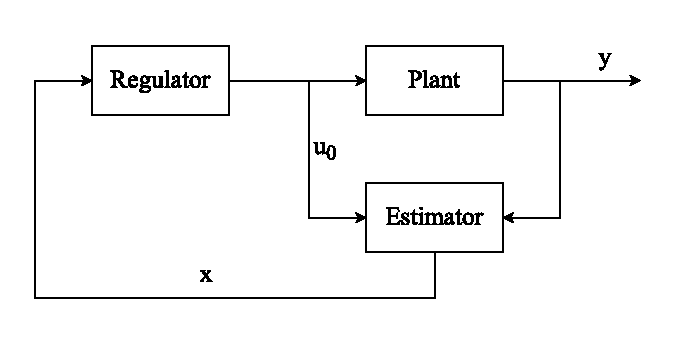
\includegraphics[scale=1.0]{LQG.pdf}
\caption{LQG control schematic}
\label{fig_lqg}
\end{figure}
The LQR and LQG controllers are two of the most fundamental results in Optimal Control theory \cite{robust}. In the next section we discuss Model Predictive Control (MPC) which is a generalisation of the controllers we have discussed so far.

\subsubsection{Model Predictive Control}
Model Predictive Control (MPC) is the constrained generalisation of the LQR controller. It is widely used industry and has been the subject of a significant amount of scholarly research. We introduce the classic deterministic linear MPC in (\ref{eq_mpc_problem}) with control/prediction horizon $N$.
\begin{equation}
\begin{aligned}
&\underset{\mathbf{u}}{\text{min }} V(x_0, \mathbf{u}) = \frac{1}{2}\sum_{k=0}^{N-1} \left( x_k^TQx_k + u_k^TRu_k \right) + \frac{1}{2}x_N^TP_fx_N \\
& \text{subject to } x_{t+1} = Ax_t+Bu_t \\
& \text{and } d^Tx_t + e \geq 0 ~\forall~t=1, 2,...,N \\
\end{aligned}
\label{eq_mpc_problem}
\end{equation}
It is straightforward to incorporate more constraints of the form $d_i^Tx_t + e_i \geq 0$ if required. The structure of (\ref{eq_mpc_problem}) is important: the objective function is quadratic and the constraints are linear. There are two primary benefits of this structure. Firstly, the problem is provably convex which means that if a minimum is found it is the global minimum. Secondly, (and as a consequence of the first benefit) this allows for the use of specialised Quadratic Programming (QP) techniques which are fast and reliable. 

Recent advances in QP algorithms, like the Interior Point algorithm, have made it possible to solve QP problems almost as fast as Linear Programming (LP) problems. These solvers typically exploit the sparseness structure inherent in problems like (\ref{eq_mpc_problem}) \cite{mac}. Thus, it is desirable to make use of these solvers wherever possible by ensuring that the underlying QP structure is not lost when modifications are made to the algorithm.

Finally, the stability and robustness of deterministic linear MPC is well studied and understood in modern literature. See \cite{raw} and \cite{mac} for details. Thus, it is likewise desirable to exploit this knowledge rather than attempt to derive an MPC with completely different or new characteristics.

We will continue our study of linear MPC in later sections.

\subsection{Matrix Identities}
\label{sec_block}
It will be useful in a later section to have access to a block matrix inversion formula. We state the result without proof and refer the reader to \cite{jang} for more details.
\begin{thrm}
\textbf{Block Matrix Inversion} Suppose we have a square block matrix of the form $\begin{pmatrix}
A & b \\ c^T & d
\end{pmatrix}
$ where $A$ is an invertible matrix; $b$ and $c$ are conforming vectors; and $d$ is a real number. Then the identity in (\ref{eq_block2}) holds with $p = (d-c^TA^{-1}b)$.
\begin{equation}
\begin{pmatrix}
A & b \\ c^T & d
\end{pmatrix}^{-1} = \begin{pmatrix}
A^{-1}(I+p^{-1}bc^TA^{-1}) & -p^{-1}A^{-1}b \\ -p^{-1}c^TA^{-1} & p^{-1}
\end{pmatrix}
\label{eq_block2}
\end{equation}
\label{thrm_block_inv}
\end{thrm}
\section{Hidden Markov Models}
\label{sec_hmm}
In this section we consider probabilistic Graphical Models of the form shown in Figure \ref{fig_linmod}. We assume that  $(X_0, X_1,...)$ are each $n$ state discrete random variables and that $(Y_0, Y_1,...)$ are each $m$ state discrete random variables. Models of this form are classically called Hidden Markov Models (HMMs).
\begin{figure}[H] 
\centering
\begin{tikzpicture}

  % Define nodes
  \node[obs] (ya) {$Y_{0}$};
  \node[latent, above=of ya]  (xa) {$X_{0}$};
  \node[obs, right=of ya] (yb) {$Y_{1}$};
  \node[latent, above=of yb, right=of xa]  (xb) {$X_1$};
  
  % Connect the nodes
  \edge {xa} {ya};
  \edge {xa} {xb};
  \edge {xb} {yb};
  
\end{tikzpicture}
\caption{Graphical Model used in this section.}
\label{fig_linmod}
\end{figure}
Intuitively, this model represents the situation where we are not sure about the state of the world but we can observe some facet of it. At each time step our state changes stochastically according to the transition function. A new observation is (stochastically) generated from our new state. Generally, we attempt to infer the state of the world given the observations. Note that at each new time step we create two new random variables $X_t, Y_t$.

In this section we briefly describe Markov Models because they link back to previous work done by the Chemical Engineering Department at the University of Pretoria. We focus on Hidden Markov Models for the remainder of the section because the techniques we develop here generalise to Latent Dynamical Systems which we discuss in Section \ref{sec_inf_lin_mods}. 

\subsection{Markov Models}
A first order Markov Model (sometimes called a Markov Chain) is shown in Figure \ref{fig_markov_chain}. Using the chain rule for Bayesian Networks (Definition \ref{def_chain_rule_bayes}) we can immediately write down the joint probability distribution as shown in (\ref{eq_markov_chain_joint}).
\begin{equation}
P(X_{0:T}) = \Pi_{t=1}^T P(X_t|X_{t-1}) \text{ with } P(X_0|X_{-1}) = P(X_0)
\label{eq_markov_chain_joint}
\end{equation}  
\begin{figure}[H] 
\centering
\begin{tikzpicture}

  % Define nodes
  \node[latent]  (xa) {$X_{0}$};
  \node[latent, right=of xa]  (xb) {$X_{1}$};
  \node[latent, right=of xb]  (xc) {$\hdots$};
  \node[latent, right=of xc]  (xd) {$X_{T-1}$};
  \node[latent, right=of xd]  (xe) {$X_{T}$};
  % Connect the nodes
  \edge {xa} {xb};
  \edge {xb} {xc};
  \edge {xc} {xd};
  \edge {xd} {xe};
\end{tikzpicture}
\caption{First Order Markov Chain.}
\label{fig_markov_chain}
\end{figure}
This model describes the forward propagation of a discrete random variable through time. It is interesting to study the marginal distribution of $P(X_T)$ as it evolves through time. By d-separation we know that $X_t \indep X_{0:t-2} | X_{t-1}$. Thus, we only have to marginalise out the previous time step to compute the required distribution as shown in (\ref{eq_markov_chain_marg}).
\begin{equation}
P(X_T) = \sum_{x_{T-1}} P(X_T, x_{T-1}) = \sum_{x_{T-1}} P(x_{T-1})P(X_T|x_{T-1})
\label{eq_markov_chain_marg}
\end{equation}
Since we know that the transition function is a row stochastic $n \times n$ matrix (the random variable has $n$ discrete states) we can write (\ref{eq_markov_chain_marg}) in vector notation (\ref{eq_markov_chain_marg_vec}). Note that $P(X_T)$ is a discrete random variable and can thus be expressed as a stochastic column vector i.e. $\sum_i P(x_t=i) = 1$.
\begin{equation}
P(X_t) = \mathbf{p}_t = \mathbf{A}\mathbf{p}_{t-1} = \mathbf{M}^{t-1}\mathbf{p}_1
\label{eq_markov_chain_marg_vec}
\end{equation}
We have implicitly rewritten (\ref{eq_markov_chain_marg_vec}) in recursive format. Thus, we have a recursive expression for the marginal distribution of $X$. If, as $T \rightarrow \infty$, we have that $\mathbf{p}_{t \rightarrow \infty} = \mathbf{p}_{\infty}$ exists and is independent of $\mathbf{p}_0$ we call $\mathbf{p}_{\infty}$ the equilibrium distribution of the chain. 

We define the stationary distribution, in matrix notation, by (\ref{eq_markov_chain_stationary}).
\begin{equation}
\mathbf{p}_{\infty} = \mathbf{A}\mathbf{p}_{\infty}
\label{eq_markov_chain_stationary}
\end{equation}
Recalling the definition of the eigenvalue problem we see that the stationary distribution is just the eigenvector corresponding to the unit eigenvalue of $\mathbf{A}$. While this model may seem simplistic it is the foundation of Google's PageRank algorithm \cite{google}.  Intuitively $\mathbf{p}_\infty$ represents the steady state probability distribution of the random variable $X$ as it is propagated through time by the transition function $A$. See the work by Streicher, Wilken and Sandrock for an application specifically geared towards Chemical Engineering \cite{streicher}.

\subsection{Hidden Markov Models}
Hidden Markov Models extend Markov Models by incorporating the observed random variables $(Y_0, Y_1,...)$ as shown in Figure \ref{fig_linmod}. At each time step it is now possible to observe the random variable $Y_t$ which gives more information about the state of $X_t$. We are still in the setting of discrete random variables. It is not necessary to restrict $(Y_0, Y_1,...)$ to be discrete but we do so for the sake of simplicity here. In later sections we will model both hybrid and purely continuous systems. 

In general a Hidden Markov Model is just a specific case of the general Dynamic Bayesian Network class of Graphical Models. As such we already know that to fully specify the model we only require a prior state distribution $P(X_0)$, the transition probability function $P(X_t|X_{t-1})$, the observation (or sometimes called the emission) probability function $P(Y_t|X_t)$ and the Bayesian Network graphs of the initial time step and the next two time steps. We assume that the model's structure repeats at each time step and thus we only require the graph as shown in Figure \ref{fig_linmod}.

We assume that the transition and observation probability functions are stationary. Consequently they may be represented by the row stochastic square matrices $P(x_t=i|x_{t-1}=j) = A$ and $P(y_t=i|x_t=j) = B$. Intuitively this means that the probability of state $x_{t-1}=j$ going to state $x_{t} = i$ is $A_{ij}$. Similarly, $B_{ij}$ is the probability of observing $y_t=i$ if the underlying state is $x_t=j$.

For the purposes of this dissertation we will always assume that the model parameters are known. In Section \ref{sec_dbns_lit} the four primary inference techniques were briefly mentioned. We now derive recursive expressions for each inference technique for discrete models of the form shown in Figure \ref{fig_linmod}. The tools and techniques we develop here will be useful in the following sections. 

\subsubsection{Filtering}
The goal of filtering is to find $P(X_t|y_{0:t})$: the distribution of the current state given all the past observations. The corresponding Graphical Model is shown in Figure \ref{fig_linmod_filter_hmm}.
\begin{figure}[H] 
\centering
\begin{tikzpicture}

  % Define nodes
  \node[obs] (ya) {$Y_{0}$};
  \node[latent, above=of ya]  (xa) {$X_{0}$};
  \node[obs, right=of ya] (yb) {$\cdots$};
  \node[latent, above=of yb, right=of xa]  (xb) {$\cdots$};
  \node[obs, right=of yb] (yc) {$Y_{t-1}$};
  \node[latent, above=of yc, right=of xb]  (xc) {$X_{t-1}$};  
  \node[obs, right=of yc] (yd) {$Y_t$};
  \node[latent, above=of yd, right=of xc]  (xd) {$X_t$};  
  
  % Connect the nodes
  \edge {xa} {ya};
  \edge {xa} {xb};
  \edge {xb} {yb};
  \edge {xb} {xc};
  \edge {xc} {yc};
  \edge {xc} {xd};
  \edge {xd} {yd};

\end{tikzpicture}
\caption{Filtering Graphical Model.}
\label{fig_linmod_filter_hmm}
\end{figure}
We start the derivation by noting that $X_{t-1}$ d-separates $X_t$ from $X_{0:t-2}$. Thus $X_{t-1}$ contains all the hidden state information of the system up to and including $t-1$. This is not surprising since we have assumed a first order Markov system. This is why we only marginalise over the reduced state joint $P(X_t, X_{t-1}|y_{0:t})$.
\begin{equation}
\begin{aligned}
P(X_t| y_{0:t-1}) &= \sum_{x_{t-1}} P(X_t, x_{t-1}| y_{0:t-1})\\
&= \sum_{x_{t-1}} P(x_{t-1}|y_{0:t-1})P(X_t|y_{0:t-1}, x_{t-1})\\  
& = \sum_{x_{t-1}} P(x_{t-1}|y_{0:t-1})P(X_t|x_{t-1}) \\
\end{aligned}
\label{eq_forward_no_recur}
\end{equation}
Where the expansion followed from the chain rule of Bayesian Networks (Definition \ref{def_chain_rule_bayes} and the cancellation followed from the conditional independence assumption of the transition function. Now we define $\alpha(X_t) \equiv P(X_t | y_{0:t})$. Then (\ref{eq_forward_recur}) follows from (\ref{eq_forward_no_recur}) and by application of Bayes' Theorem (Theorem \ref{thrm_bayes}).
\begin{equation}
\begin{aligned}
\alpha(X_t) &= \frac{P(y_t|X_t, y_{0:t-1})P(X_t|y_{0:t-1})}{P(y_t|y_{0:t-1})} \\
& = \frac{P(y_t|X_t)P(X_t|y_{0:t-1})}{P(y_t|y_{0:t-1})} \\
& = \frac{P(y_t|X_t) \sum_{x_{t-1}} P(x_{t-1}|y_{0:t-1})P(X_t|x_{t-1})}{P(y_t|y_{0:t-1})} \\
& = \frac{P(y_t|X_t) \sum_{x_{t-1}} \alpha(x_{t-1})P(X_t|x_{t-1})}{P(y_t|y_{0:t-1})} \\
\end{aligned}
\label{eq_forward_recur}
\end{equation}
Note that it is not actually necessary to calculate $p(y_t|y_{0:t-1})$ as it is only a normalisation constant. We thus have a recursion relation for the filtered posterior distribution $X_t$ with initial condition $\alpha(X_1) = P(X_1, y_1) = P(X_1)P(y_1|X_1)$ as shown in (\ref{eq_forward_approx}).
\begin{equation}
\alpha(X_t) \propto P(y_t|X_t) \sum_{x_{t-1}} \alpha(x_{t-1})P(X_t|x_{t-1})
\label{eq_forward_approx}
\end{equation}

One often uses logarithms to perform the filter calculations as machine precision errors become a problem for large $t$ due to the multiplication of small fractions. The recursive filtering algorithm we derived is often called the Forwards Algorithm in literature \cite{barber}.

\subsubsection{Smoothing}
The goal of smoothing is to find $P(X_t|y_{0:T})$ for $t\leq T$: the distribution of the state at $t$ given all the past and future observations to $T$. The smoothing algorithm we study here is called the parallel smoothing algorithm. The recursion expression we derive is often called the Backwards Algorithm in literature \cite{murphy1}. The Graphical Model corresponding to this situation is shown in Figure \ref{fig_linmod_smooth_hmm}.
\begin{figure}[H] 
\centering
\begin{tikzpicture}

  % Define nodes
  \node[obs] (ya) {$Y_{0}$};
  \node[latent, above=of ya]  (xa) {$X_{0}$};
  \node[obs, right=of ya] (yb) {$\cdots$};
  \node[latent, above=of yb, right=of xa]  (xb) {$\cdots$};
  \node[obs, right=of yb] (yc) {$Y_{t}$};
  \node[latent, above=of yc, right=of xb]  (xc) {$X_{t}$};  
  \node[obs, right=of yc] (yd) {$\cdots$};
  \node[latent, above=of yd, right=of xc]  (xd) {$\cdots$};  
  \node[obs, right=of yd] (ye) {$Y_T$};
  \node[latent, above=of ye, right=of xd]  (xe) {$X_T$};  
  
  % Connect the nodes
  \edge {xa} {ya};
  \edge {xa} {xb};
  \edge {xb} {yb};
  \edge {xb} {xc};
  \edge {xc} {yc};
  \edge {xc} {xd};
  \edge {xd} {yd};
  \edge {xd} {xe};
  \edge {xe} {ye};

\end{tikzpicture}
\caption{Smoothing Graphical Model.}
\label{fig_linmod_smooth_hmm}
\end{figure}
We start by splitting the joint $P(X_t, y_{0:T}) = P(X_t, y_{0:t})P(y_{t+1:T}|X_t,y_{0:t})$ by the chain rule and using d-separation to reduce it further $P(X_t, y_{0:T}) = P(X_t, y_{0:t})P(y_{t+1:T}|X_t)$. Effectively the last step implies that future observations are independent of past observations given the current state. We defined $\beta(X_t)\equiv P(y_{t+1:T}|X_t)$ and continue the derivation in (\ref{eq_backwards_no_recur}).
\begin{equation}
\begin{aligned}
P(y_{t:T}|X_{t-1}) &= \sum_{x_t} P(y_t, y_{t+1:T}, x_t|X_{t-1}) \\
&= \sum_{x_t} P(y_{t+1:T}, x_t | X_{t-1})P(y_t| y_{t+1:T}, x_t, X_{t-1}) \\
&= \sum_{x_t} P(y_{t+1:T}, x_t | X_{t-1})P(y_t| x_t) \\
&= \sum_{x_t} P(x_t | X_{t-1})P(y_{t+1:T}| x_t,X_{t-1})P(y_t| x_t) \\
&= \sum_{x_t} P(x_t | X_{t-1})P(y_{t+1:T}| x_t)P(y_t| x_t) \\
\end{aligned}
\label{eq_backwards_no_recur}
\end{equation}
We have made judicious use of the implied independence assertions (via d-separation) of Figure \ref{fig_linmod}. Making use of the definition of $\beta$ we have (\ref{eq_backwards_recur}).
\begin{equation}
\begin{aligned}
&\beta(X_{t-1}) = \sum_{x_t} P(x_t | X_{t-1})\beta(x_t)P(y_t| x_t) \text{ for } 1 \leq t \leq T \\
&\text{with } \beta(X_T) = 1
\end{aligned}
\label{eq_backwards_recur}
\end{equation}
The recursion initial condition $\beta(X_T) = 1$ stems from Bayes' Theorem (Theorem \ref{thrm_bayes}) and the definition of $\alpha$ as shown in (\ref{eq_backwards_recur_initial}). Note that $\beta$ is not a probability function.
\begin{equation}
\begin{aligned}
P(X_T|y_{0:T}) &= \frac{P(X_T, y_{0:T})}{P(y_{0:T})} \\
&= \alpha(X_T) \beta(X_T)\\
&= P(X_T| y_{0:T}) \beta(X_T)\\
&\implies \beta(X_T) = 1
\end{aligned}
\label{eq_backwards_recur_initial}
\end{equation}
The smoothed posterior is given by applying Bayes' Theorem as shown in (\ref{eq_smooth}).
\begin{equation}
P(X_t|y_{0:T}) = \frac{\alpha(X_t)\beta(X_t)}{\sum_{x_t}\alpha(x_t)\beta(x_t)}
\label{eq_smooth}
\end{equation}
Together the $\alpha - \beta$ recursions are called the Forwards-Backwards algorithm and find extensive use in general purpose exact inference of Dynamic Bayesian Networks \cite{murphy1}.

Numerical issues may also become problematic due to the multiplication of small positive numbers. In practice it is often necessary to work in the log space to attenuate these problems \cite{barber}. 

\subsubsection{Viterbi Decoding}
The goal of Viterbi Decoding is to find $x_{0:T}^* = \underset{x_{0:T}}{\text{arg max }} P(x_{0:T}|y_{0:T})$: finding the most likely sequence of states which best describe the observations by  attempting to find the sequence $x_{0:T}$ such that the joint probability function $P(x_{0:T}, y_{0:T})$ is maximised. This is equivalent to finding $ \underset{x_{0:T}}{\text{arg max }} P(x_{0:T}|y_{0:T})$ because, if one uses the chain rule on the joint, the observations will just be a constant factor. The Graphical Model used here is similar to that of Figure \ref{fig_linmod_smooth_hmm}.

Intuitively we first attempt to find the maximum of the joint and then determine which sequence of states led to this maximal joint. By using the chain rule for Bayesian Networks we can rewrite the joint maximisation problem as in (\ref{eq_viterbi_joint}).
\begin{equation}
\begin{aligned}
\underset{x_{0:T}}{\text{max }} P(x_{0:T}, y_{0:T}) &= \underset{x_{0:T}}{\text{max }} \Pi_{t=1}^T P(y_t|x_t) P(x_t|x_{t-1})\\
&= \left(\underset{x_{0:T-1}}{\text{max }} \Pi_{t=1}^{T-1} P(y_t|x_t) P(x_t|x_{t-1}) \right) \underset{x_{T}}{\text{max }} P(y_T|x_T) P(x_T|x_{T-1})
\end{aligned}
\label{eq_viterbi_joint}
\end{equation}
Defining $\mu(X_{t-1}) \equiv \underset{x_{t}}{\text{max }} P(y_t|x_t) P(x_t|x_{t-1})$ we can rewrite (\ref{eq_viterbi_joint}) as (\ref{eq_viterbi_max_factor_mu}).
\begin{equation}
\underset{x_{0:T}}{\text{max }} P(x_{0:T}, y_{0:T}) =\underset{x_{0:T-1}}{\text{max }} \Pi_{t=1}^{T-1} P(y_t|x_t) P(x_t|x_{t-1}) \mu(x_{T-1})
\label{eq_viterbi_max_factor_mu}
\end{equation}
Thus we have a recursive expression to find the value of the joint under the most likely sequence of states given the observations as shown in (\ref{eq_viterbi_recur}).
\begin{equation}
\begin{aligned}
&\mu(x_{t-1}) = \underset{x_{t}}{\text{max }} P(y_t|x_t) P(x_t|x_{t-1}) \mu(x_t) \text{ for } 2 \leq t \leq T \\
&\text{with } \mu(x_T) = 1 
\end{aligned}
\label{eq_viterbi_recur}
\end{equation}
The recursive expression in (\ref{eq_viterbi_recur}) implies that the effect of maximising over over the previous time step can be compressed into a message (a function) of the current time step. Effectively we pass theses messages backward in time to find the maximum joint in terms of $x_0$. We then find the state which maximises this joint and pass this message forward.  Continuing in this way, we have (\ref{eq_viterbi_recur_forward}).
\begin{equation}
\begin{aligned}
x_1^* &= \underset{x_{1}}{\text{arg max }}P(y_1|x_1)P(x_1)\mu(x_1) \\
x_2^* &= \underset{x_{2}}{\text{arg max }}P(y_2|x_2)P(x_2|x_1^*)\mu(x_2) \\
&~~\vdots \\
x_t^* &= \underset{x_{t}}{\text{arg max }}P(y_t|x_t)P(x_t|x_{t-1}^*)\mu(x_t)
\end{aligned}
\label{eq_viterbi_recur_forward}
\end{equation}
This algorithm is called the Viterbi algorithm. It is computationally efficient since the optimisations occur only on a single variable. Readers familiar with Dynamic Programming will recognise that we have effectively performed a variant of Dynamic Programming in the preceding derivation.

\subsubsection{Prediction}
The goal of prediction is to find $P(X_{t+1}|y_{0:t})$ and $P(Y_{t+1}|y_{0:t})$: the predicted hidden and observed state given all the previous observations. The one step ahead prediction expression for both the states and observations is derived here. The Graphical Model corresponding to the state prediction is shown in Figure \ref{fig_linmod_pred_hmm}. 
\begin{figure}[H] 
\centering
\begin{tikzpicture}

  % Define nodes
  \node[obs] (ya) {$Y_{0}$};
  \node[latent, above=of ya]  (xa) {$X_{0}$};
  \node[obs, right=of ya] (yb) {$\cdots$};
  \node[latent, above=of yb, right=of xa]  (xb) {$\cdots$};
  \node[obs, right=of yb] (yc) {$Y_{t}$};
  \node[latent, above=of yc, right=of xb]  (xc) {$X_{t}$};  
  \node[latent, above=of yd, right=of xc]  (xd) {$X_{t+1}$};  
  
  % Connect the nodes
  \edge {xa} {ya};
  \edge {xa} {xb};
  \edge {xb} {yb};
  \edge {xb} {xc};
  \edge {xc} {yc};
  \edge {xc} {xd};
  
\end{tikzpicture}
\caption{State Prediction Graphical Model.}
\label{fig_linmod_pred_hmm}
\end{figure}

We again start by noticing that given all the observations  up to time $t$ the current state d-separates  all previous states. Thus, to infer information about the next state we only need to marginalise out the current state $X_t$. Furthermore, the next state d-separates the next observation from all the previous states. Thus, to infer information about the next observation we additionally only need to marginalise out $X_{t+1}$.

We start with predicting the next state distribution. We have applied the chain rule, the independence assertions and used the definition of $\alpha$ to derive (\ref{eq_prediction_state}).
\begin{equation}
\begin{aligned}
P(X_{t+1}|y_{0:t}) &= \sum_{x_t} P(X_{t+1}, x_t|y_{0:t}) \\
&= \sum_{x_t} P(x_t|y_{0:t})P(X_{t+1}|x_t, y_{0:t}) \\
&= \sum_{x_t} P(x_t|y_{0:t})P(X_{t+1}|x_t) \\
&= \sum_{x_t} \alpha(x_t)P(X_{t+1}|x_t) \\
\end{aligned}
\label{eq_prediction_state}
\end{equation}
Clearly the state prediction uses the filtered state estimate and projects that forward using the transition function.

Next we derive the observation prediction. Again we apply the chain rule, use the independence assertions and use the definition of $\alpha$ to derive (\ref{eq_prediction_observation}).
\begin{equation}
\begin{aligned}
P(Y_{t+1}|y_{0:t}) &= \sum_{x_t, x_{t+1}} P(x_{t+1}, x_t, Y_{t+1}|y_{0:t})\\
&= \sum_{x_t, x_{t+1}} P(x_t|y_{0:t})P(x_{t+1}, Y_{t+1}|y_{0:t}, x_t) \\
&= \sum_{x_t, x_{t+1}} P(x_t|y_{0:t})P(x_{t+1}|y_{0:t}, x_t)P(Y_{t+1}|y_{0:t}, x_t, x_{t+1}) \\
&= \sum_{x_t, x_{t+1}} P(x_t|y_{0:t})P(x_{t+1}|x_t)P(Y_{t+1}|x_{t+1}) \\
&= \sum_{x_t, x_{t+1}} \alpha(x_t)P(x_{t+1}|x_t)P(Y_{t+1}|x_{t+1}) \\
\end{aligned}
\label{eq_prediction_observation}
\end{equation}
Clearly the observation prediction is just an extension of the state prediction. We effectively just predict the next state and use the observation function to predict the observation distribution.

It is pleasing that the prediction expressions are closely related to each other and effectively only depend on the filtered state estimate and the transition or observation functions. This realisation hold for more general problems and will become important when we consider controlling the system. More on this later.

\subsection{Burglar Localisation Problem}
While the focus of this dissertation is not on HMM type problems it is nevertheless instructive to consider a simple example to build some intuition about inference of random variables. Thus, it is desirable to conduct a numerical experiment using the previously derived inference techniques. The type of problem we consider here is a localisation problem. This type of problem (and its extensions) has many applications in robotics and object tracking.

The problem is taken from Chapter 23 in Barber's book \textit{Bayesian Reasoning and Machine Learning} \cite{barber}. Briefly, it is necessary to infer the location of a burglar in your house given observations (noises) you perceive from an adjoining room. You discretise the room the burglar is in into $n^2$ blocks. The room is then the discrete random variable $X$. You observe two distinct types of noises: creaks and bumps. From the knowledge of your house you know which blocks are likely to creak and which are likely to bump if the burglar is on that block i.e. if the random variable $X$ is in a specific state. This is shown in Figure \ref{fig_burlgar_observations}: a dark block indicates it is likely to emit a noise with probility 0.9 and a light block will emit a noise with probability 0.01 if the burglar is on that block. The noises are independent of each other.
\begin{figure}[H] 
\centering
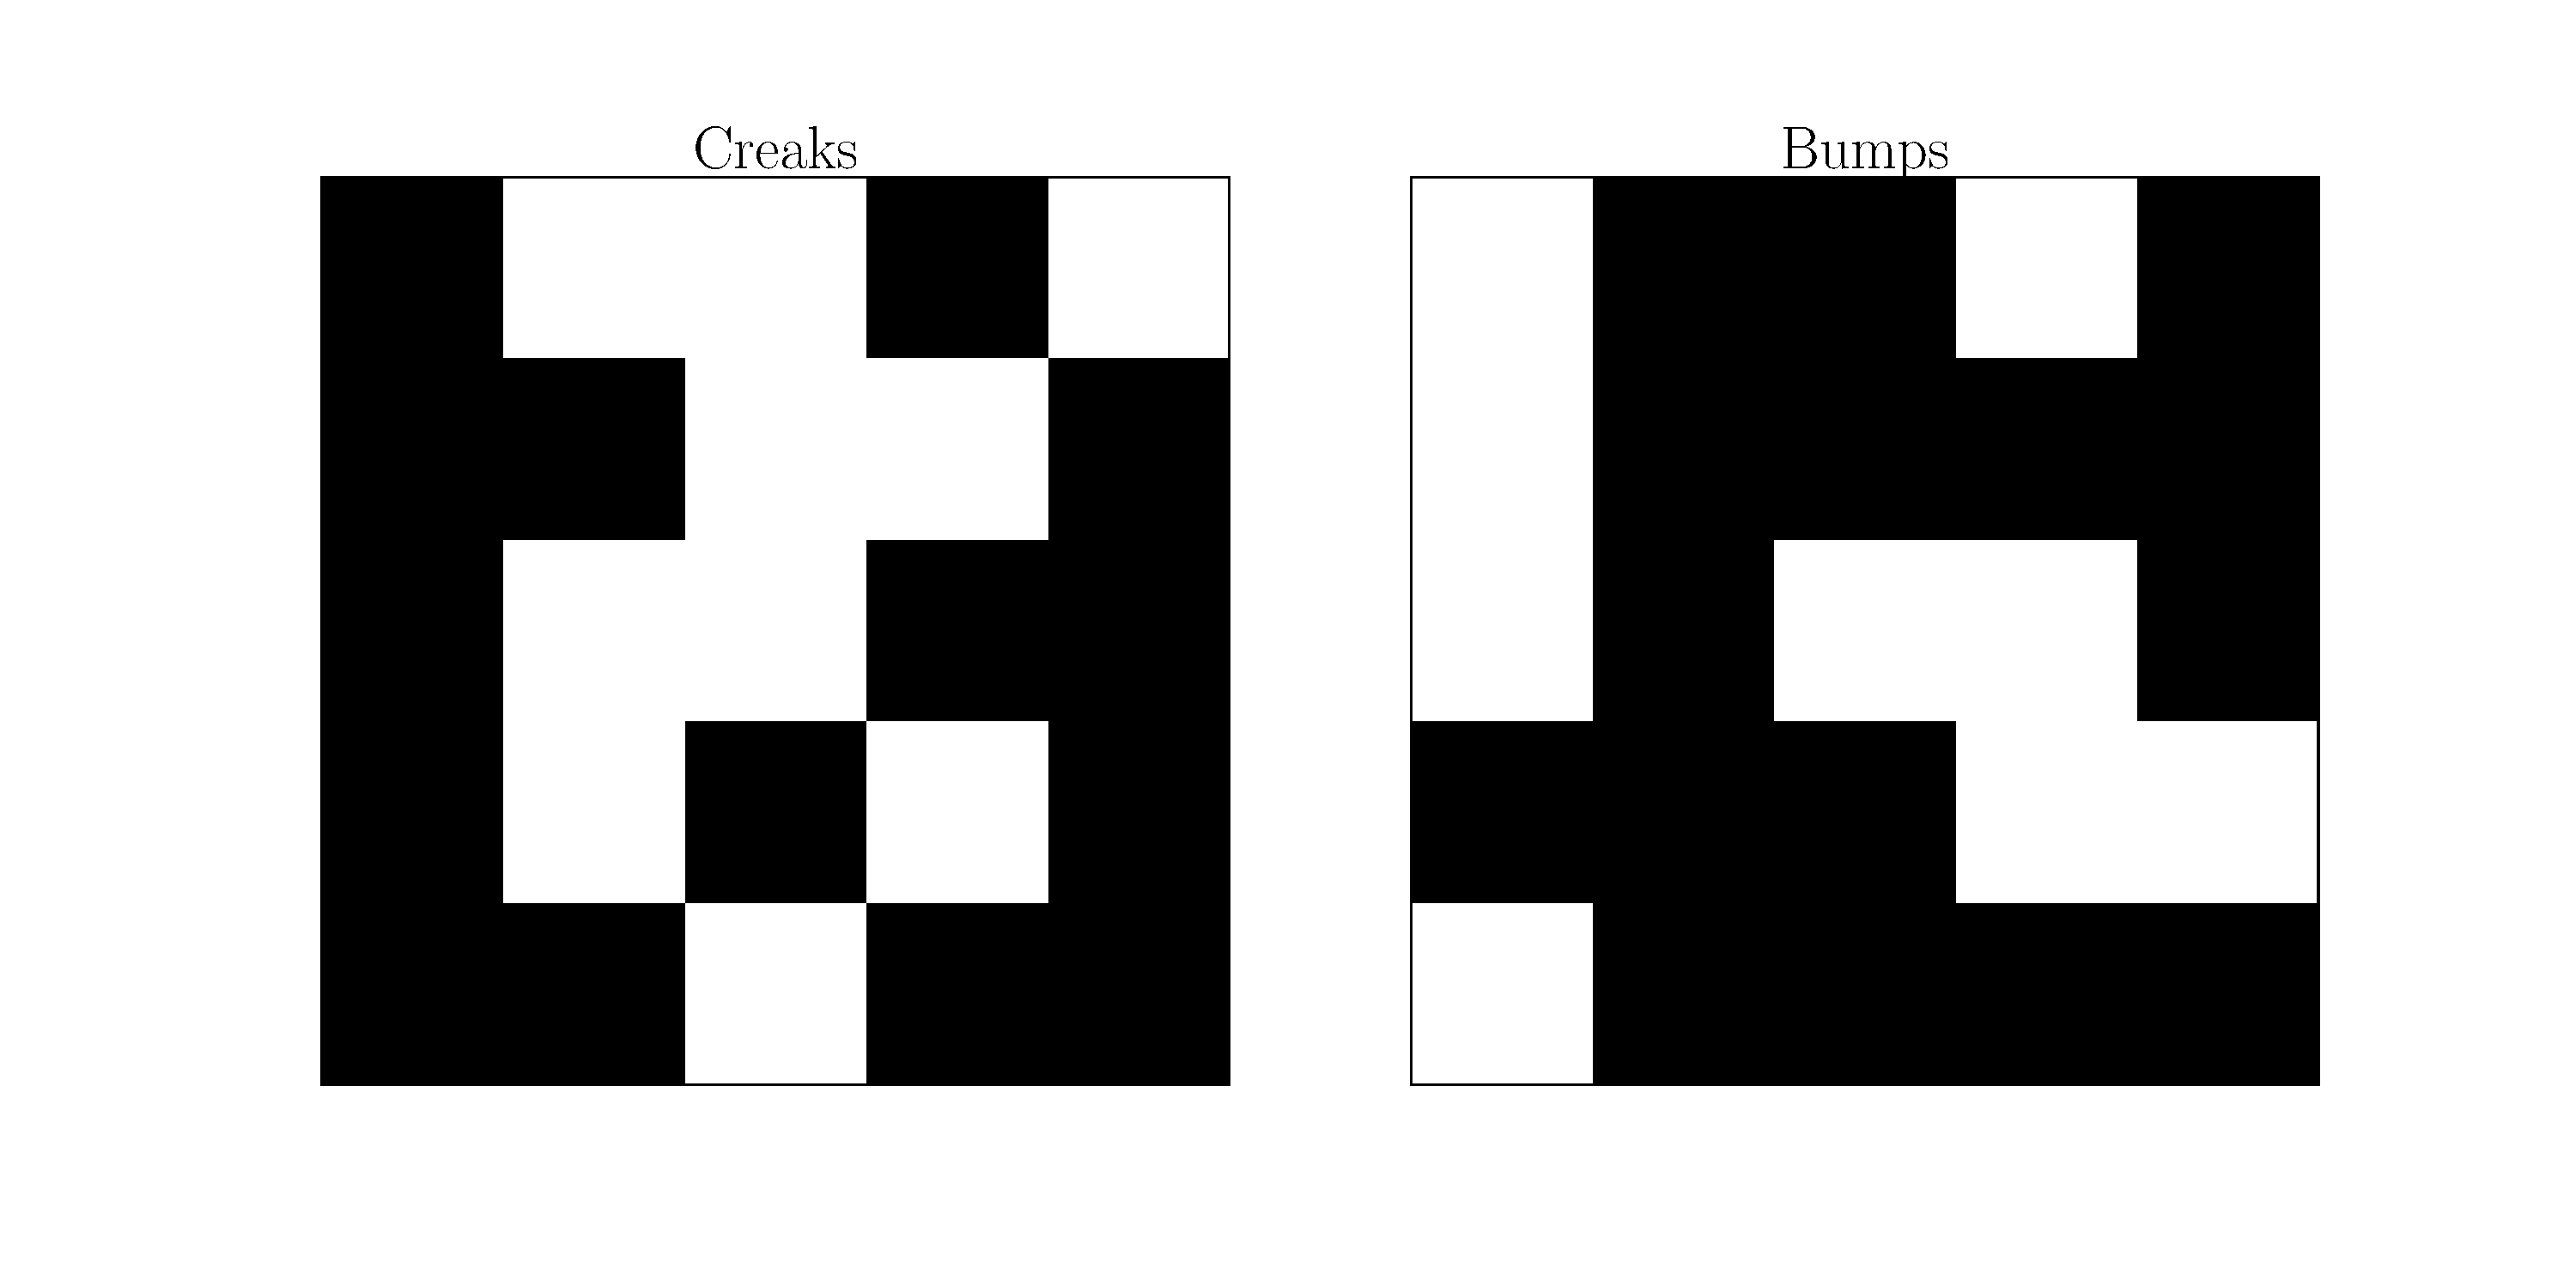
\includegraphics[scale=0.20]{burglar_observations.pdf}
\caption{Burglar Problem Observations}
\label{fig_burlgar_observations}
\end{figure}
The burglar moves up, down, left and right with equal probability where appropriate. See Barber for more details on the example. It is necessary to perform inference to determine the path of the burglar both in real time and with the benefit of hindsight. Applying the inference techniques we developed earlier results in Figure \ref{fig_burglar_inference}. 
\begin{figure}[H] 
\centering
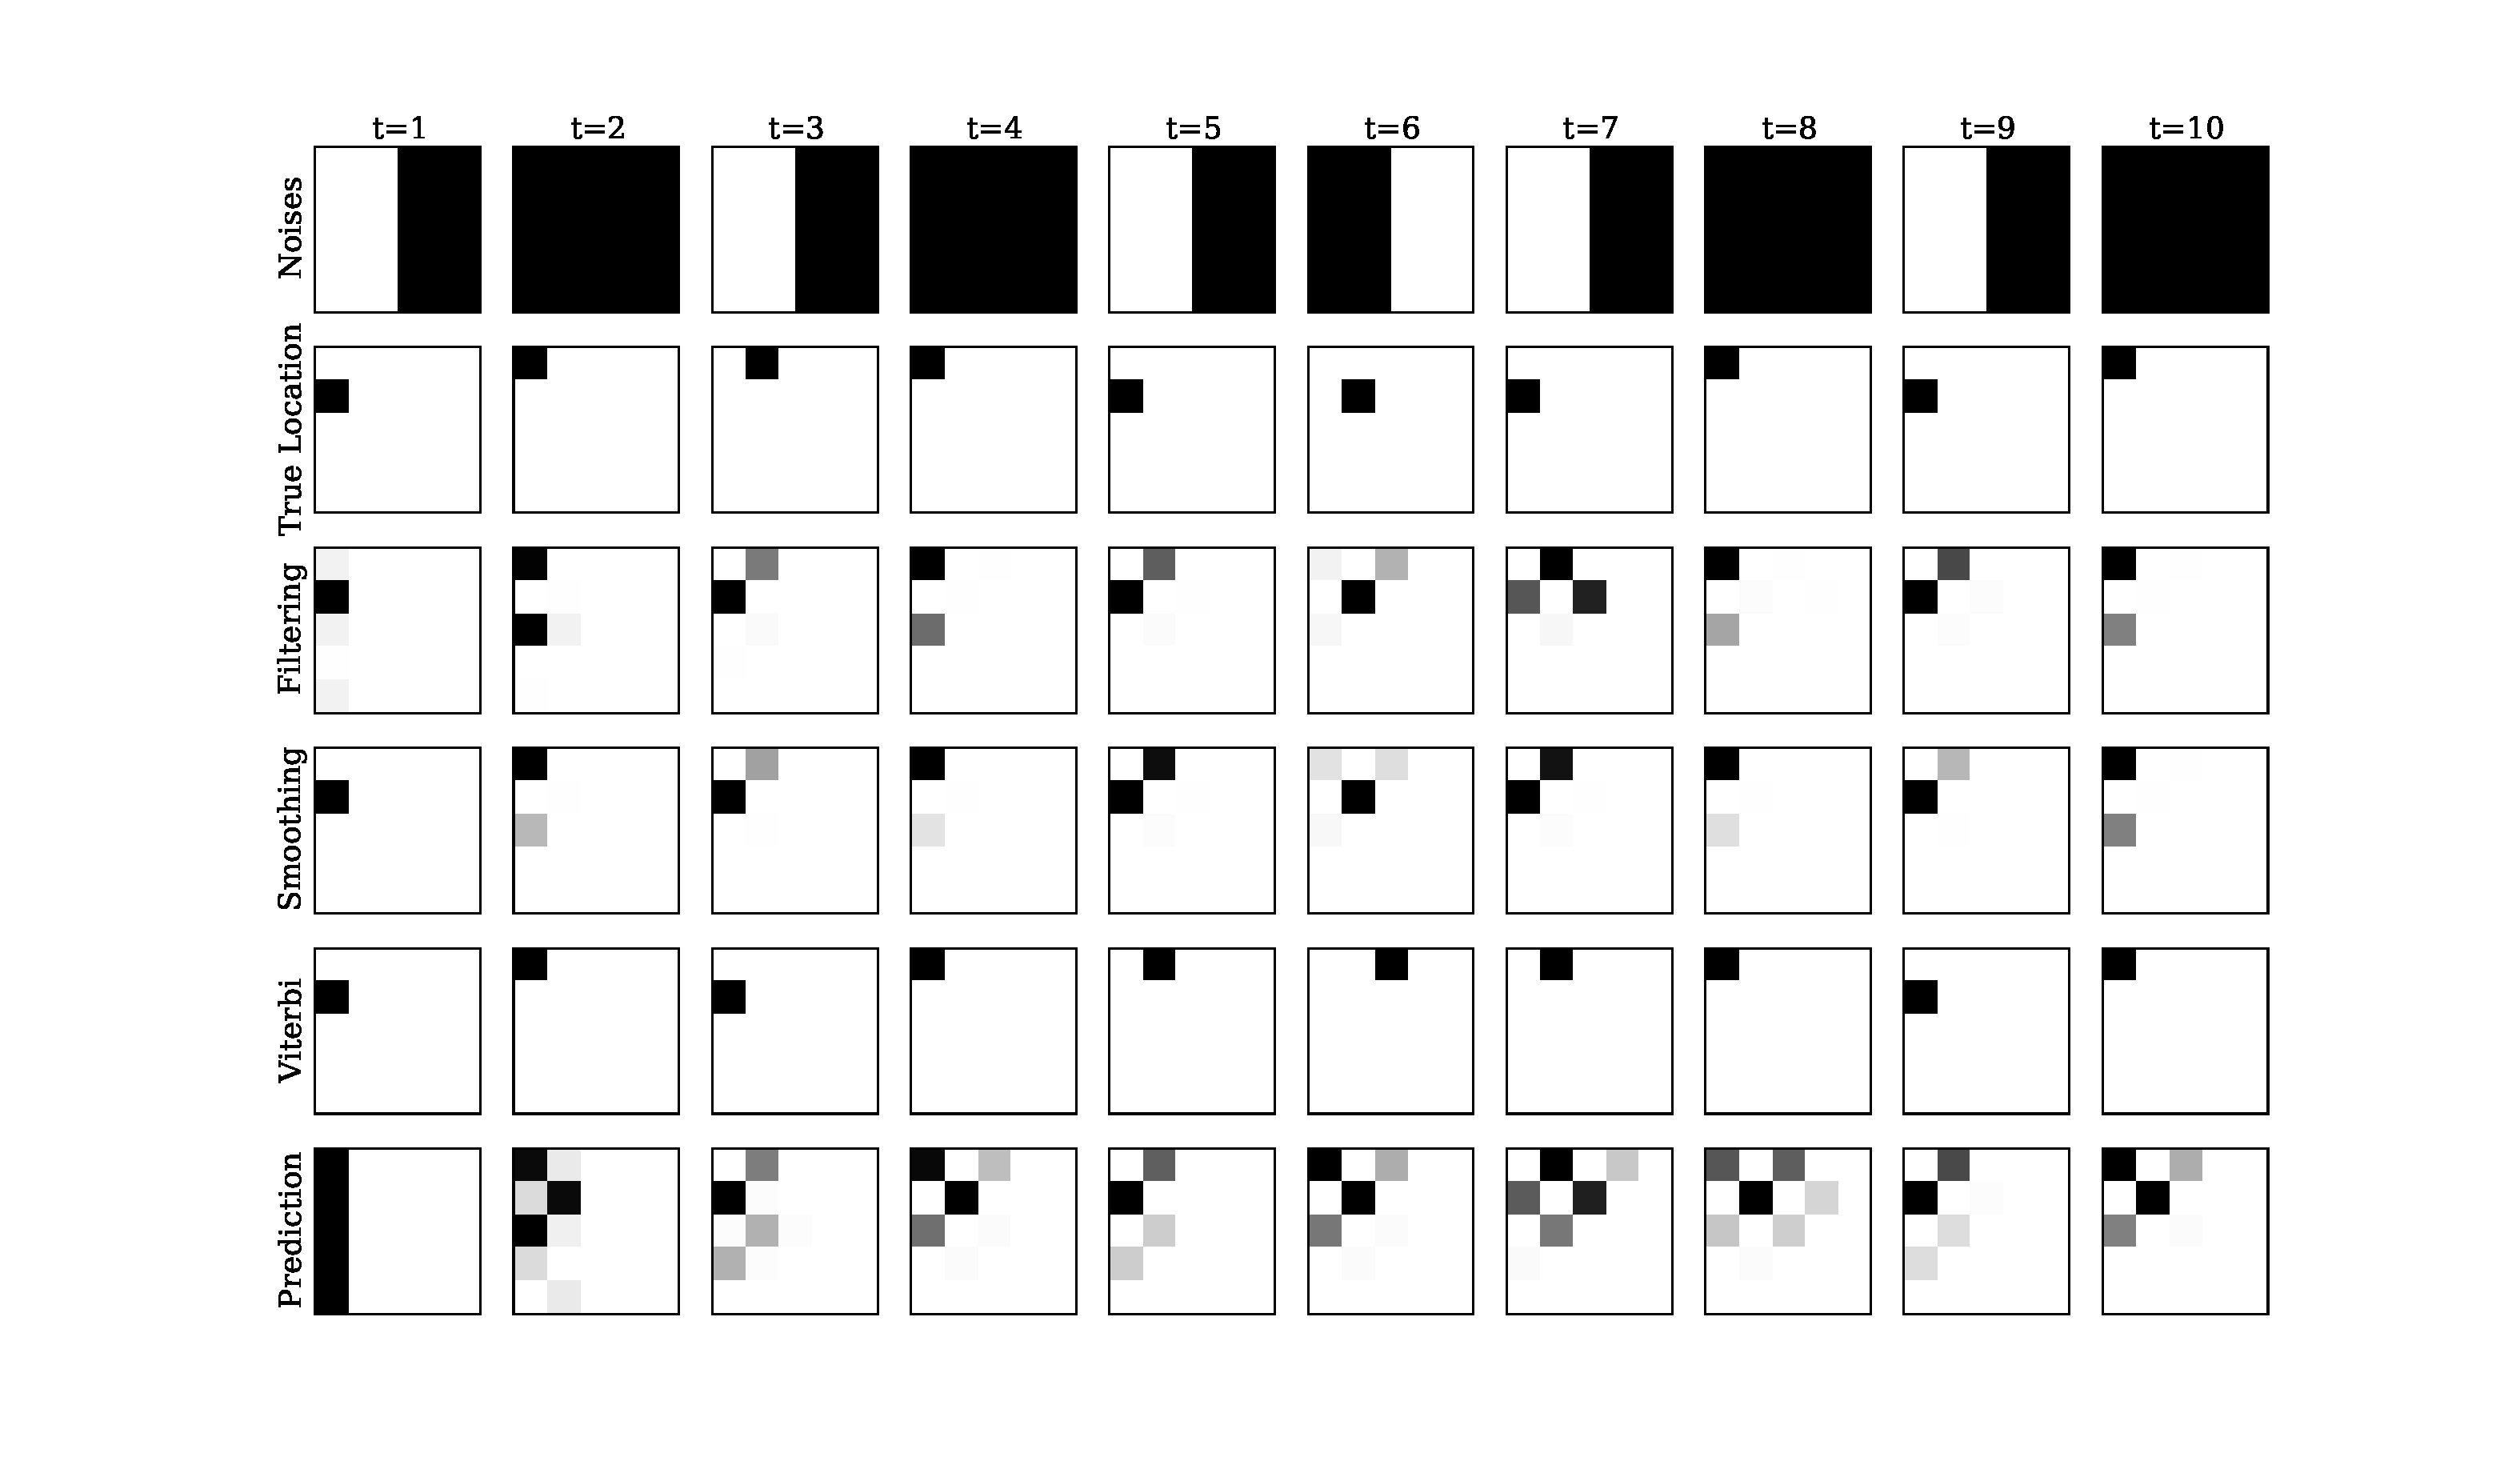
\includegraphics[scale=0.29]{burglar_inference.pdf}
\caption{Burglar Problem: Filter, Smoothing, Viterbi Decoding and Prediction}
\label{fig_burglar_inference}
\end{figure}
In this context filtering means we estimate the location of the burglar given all the past observations at the current time step. This inference can be done on-line. Smoothing means we attempt to estimate his position with hindsight given all the observations starting from the first time step and moving forwards. In Viterbi decoding we attempt to estimate the most likely path path of the burglar. Finally the prediction algorithm is self-explanatory.

It is interesting to note that smoothed posterior converges to the filtered posterior near the end of the time window. Reflecting on the expression for smoothing this is not surprising since at $t=T$ the smoothing component of the Forwards-Backwards algorithm is unity. Therefore we see that the smoothed state estimate converges to the filtered state estimate as $t$ approaches $T$.

It is also interesting to note that the prediction algorithm is very much dependent on the quality of the transition function. The four block pattern readily apparent in the prediction distribution originates from the transition function (the burglar is equally likely to move in any direction). This strongly implies that the closer the transition function is to reality the better our predictions will be.

Finally, it is important to understand the benefit of using this approach as opposed to the exhaustive ``if this then that" approach. Firstly, the latter approach scales exponentially with the number of variables because one would need to fully consider all the possibilities to infer any sort of belief. Secondly, the former approach has an associated probability distribution: the certainty of our inferred belief is automatically quantified e.g. the darker the blocks the more sure we are about our inference. Thus, the techniques we developed make room for uncertainty about the correctness of the answer.

Hidden Markov Models are very powerful and have found many uses e.g. speech recognition, object tracking and bio-informatics \cite{barber}. Many extensions of the basic model (see Figure \ref{fig_linmod}) exist which are much more expressive. However, we are interested in modelling and reasoning about continuous random variables. For such applications the Hidden Markov Model, due to the discrete assumption, is inappropriate. Fortunately, the techniques investigated in this section carry over to the continuous case as we will see next.  

\documentclass[../masters.tex]{subfiles}

\begin{document}
\graphicspath{{./imgs/}{../imgs/}} %look for images

\section{CSTR Model}
In this section we introduce the model we will use to illustrate the techniques we develop in this dissertation. The model is a simple continuously stirred tank reactor (CSTR) undergoing an exothermic, irreversible first order reaction where $A \rightarrow B$. A schematic diagram of the reactor is shown in Figure \ref{fig_cstr_diagram}. The model is taken from literature \cite{cstrmodel}.
\begin{figure}[H] 
\centering
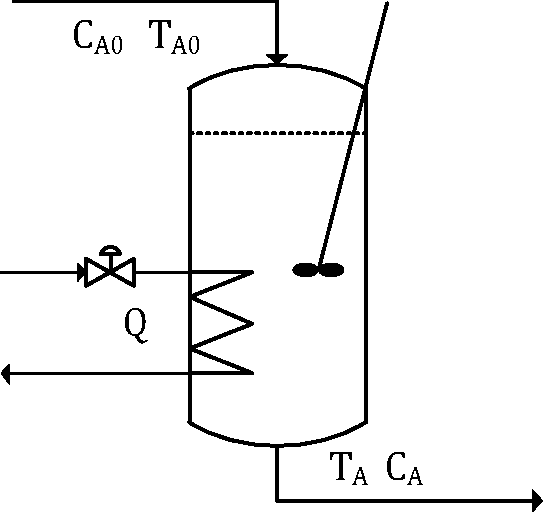
\includegraphics[scale=0.8]{cstr_diagram.pdf}
\caption{Diagram of a simple CSTR where the heat added to system is the only manipulated variable.}
\label{fig_cstr_diagram}
\end{figure}
The state space equations describing the reactor are shown in (\ref{eq_cstrmodel}) with parameters shown in Table \ref{tab_params}. The meaning of the variables is what one would expect from an intuitive understanding: $C_A$ is the concentration of species $A$, $T_R$ is the temperature of the CSTR and $Q$ is the heat added (or removed for negative $Q$) from the CSTR.
\begin{equation}
\begin{aligned}
\dot{C_A} &= f(C_A, T_R) =  \frac{F}{V}\left( C_{A0}-C_A \right) - k_0e^{\frac{-E}{RT_R}}C_A \\
\dot{T_R} &= g(C_A, T_R) = \frac{F}{V}\left(T_{A0}-T_A\right) + \frac{-\triangle H}{\rho C_p}k_0e^{\frac{-E}{RT_R}}C_A + \frac{Q}{\rho C_p V}
\end{aligned}
\label{eq_cstrmodel}
\end{equation}
\begin{table}[H]
\begin{center}
\begin{tabular}{c c c c}
\hline
$V$ & $~5.0~m^3$ & $R$ & $~8.314~\frac{kJ}{kmol.K}$ \\
$C_{A0}$ & $~1.0~\frac{kmol}{m^3}$ &$T_{A0}$ & $~310~K$ \\
$\triangle H$ & $~-4.78\times 10^{4}~\frac{kJ}{kmol}$ & $k_{0}$ & $~72\times 10^{7}~\frac{1}{min}$ \\
$E$ & $~8.314\times 10^4~\frac{kJ}{kmol}$ & $C_{p}$ & $~0.239~\frac{kJ}{kg.K}$ \\
$\rho$ & $~1000~\frac{kg}{m^3}$ & 
$F$ & $~100\times 10^{-3}~\frac{m^3}{min}$ \\
\hline
\end{tabular}
\caption{CSTR parameters}
\label{tab_params}
\end{center}
\end{table}
The CSTR model is a familiar control example. Similar models may be found in \cite{du}\cite{cervantes}\cite{pan}\cite{yazdi}. We use this model because it is low dimensional yet complex enough to illustrate the principles we investigate. Note that we have increased the volume of the reactor and reduced the rate constant from the reactor we quoted in literature. This is primarily to adjust the time scale of the transient response to be in the order of minutes and not milliseconds.

\subsection{Qualitative Analysis}
In this section we use standard mathematical tools, as found in \cite{edwardsandpenny}, to analyse the qualitative behaviour of the CSTR. By inspecting (\ref{eq_cstrmodel}) we see that the model is coupled and non-linear. By solving (\ref{eq_cstr_statpoints}) we see that for nominal operating conditions ($Q = 0$) there exist 3 operating points (critical points) as shown in Table \ref{tab_nominalstats}.
\begin{equation}
\begin{aligned}
0&= \frac{F}{V}\left( C_{A0}-C_A \right) - k_0e^{\frac{-E}{RT_R}}C_A \\
0 &= \frac{F}{V}\left(T_{A0}-T_A\right) + \frac{-\triangle H}{\rho C_p}k_0e^{\frac{-E}{RT_R}}C_A + \frac{Q}{\rho C_p V}
\end{aligned}
\label{eq_cstr_statpoints}
\end{equation}
\begin{table}[H]
\begin{center}
\begin{tabular}{c c c c}
\hline
Critical Point & $C_A$ & $T_R$ & Stability\\
\hline
$\left(C_A^1, T_R^1\right)$ & 0.0097 & 508.0562 & Stable Improper Node\\
$\left(C_A^2, T_R^2\right)$ & 0.4893 & 412.1302 & Unstable Saddle Point \\
$\left(C_A^3, T_R^3 \right)$ & 0.9996 & 310.0709 & Stable Improper Node \\
\hline
\end{tabular}
\caption{Nominal operating points for  the CSTR}
\label{tab_nominalstats}
\end{center}
\end{table}
The stability of the operating points were found by linearising (\ref{eq_cstrmodel}) and computing the eigenvalues of the Jacobian, shown in (\ref{eq_jacobian}), at each critical point.
\begin{equation}
J(C_A, T_R) = \begin{pmatrix}
-\frac{F}{V} - k_0e^{\frac{-E}{RT_R}} & - k_0e^{\frac{-E}{RT_R}}C_A\left(\frac{E}{RT_R^2}\right) \\
\frac{-\triangle H}{\rho C_p}k_0e^{\frac{-E}{RT_R}} & -\frac{F}{V} + \frac{-\triangle H}{\rho C_p}k_0e^{\frac{-E}{RT_R}}C_A\left(\frac{E}{RT_R^2}\right) 
\end{pmatrix}
\label{eq_jacobian}
\end{equation}
In Figure \ref{fig_cstr_op_curve} we see the operating curve for the CSTR. The curve resembles the classical CSTR operating curve with all the associated potential control complexity e.g. it is possible for one set of control inputs to result in two stable operating points. This occurs due to the two stable critical points (for $Q\in (-906, 1145)$) of the system and is called input multiplicity \cite{luyben}. 

Also note that the obvious bifurcation parameter for this system is the heat input $Q$. For $Q = -906$ kJ/min we see that we no longer have three critical points but only two, and for $Q < -906$ kJ/min we only have one critical point. Likewise, for $Q = 1145$ kJ/min we see that we only have two critical points and for $Q > 1145$ kJ/min we only have one critical point. The stability of these points are shown in Table \ref{tab_bifurc}.  
\begin{figure}[H] 
\centering
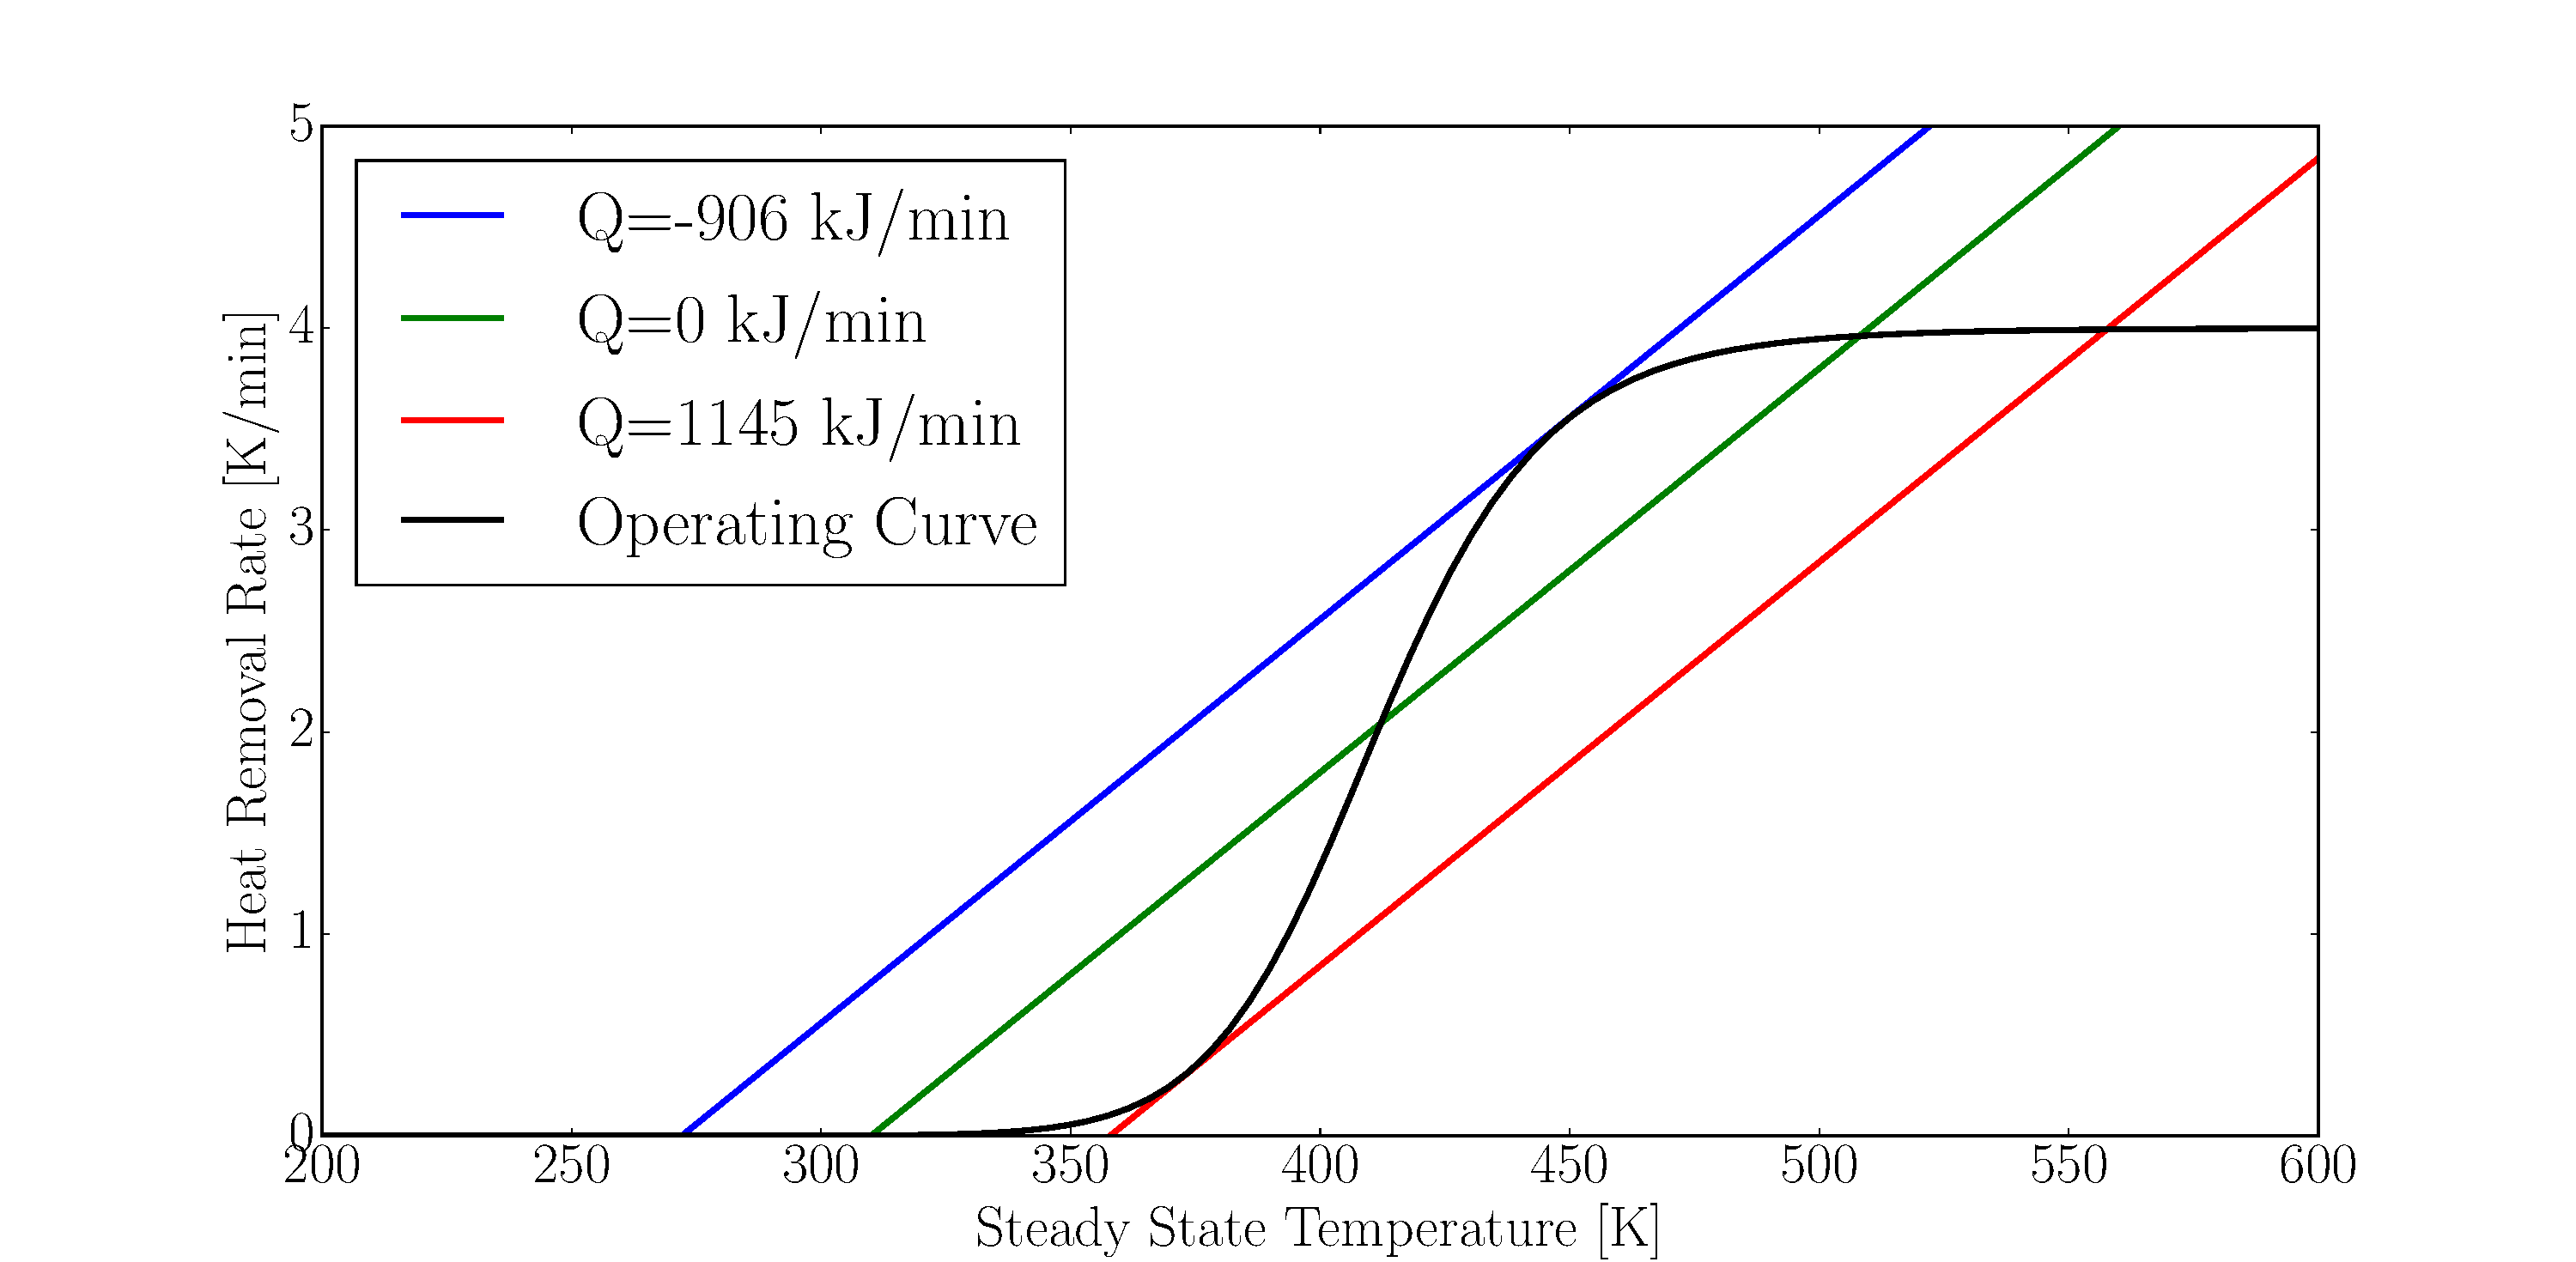
\includegraphics[scale=0.3]{cstr_model_op_curve.pdf}
\caption{CSTR operating curve with different input curves. Nominal operating conditions are $Q=0$ kJ/min.}
\label{fig_cstr_op_curve}
\end{figure}
\begin{table}[H]
\begin{center}
\begin{tabular}{c c c c}
\hline
Heat Input & $C_A$ & $T_R$ & Stability\\
\hline
$Q = -906$ kJ/min & 0.1089 & 450.3531 & Stable Improper Node\\
$Q = -906$ kJ/min & 0.9999 & 272.1346 & Stable Improper Node \\
$Q < -906$ kJ/min & $\backsim$ & $\backsim$ & Stable Improper Node \\
\hline
$Q = 1145$ kJ/min & 0.0017 & 557.5243 & Stable Improper Node\\
$Q = 1145$ kJ/min & 0.9263 & 372.5959 & Stable Improper Node \\
$Q > 1145$ kJ/min & $\backsim$ & $\backsim$ & Stable Improper Node \\
\hline
\end{tabular}
\caption{Bifurcation analysis of the CSTR at different heat input values.}
\label{tab_bifurc}
\end{center}
\end{table}
The multiple stable critical points for $Q\in [-906, 1145]$ kJ/min makes control of this system challenging. For example consider a situation where one starts at some point on the black line, below the green line in Figure \ref{fig_cstr_op_curve}. If one wishes to move to the high temperature low concentration stable operating point large, non-smooth, controller action will be required. By slowly heating up the CSTR the green line will gradually move to the right and this will push the system, somewhat counter-intuitively, towards the low temperature high concentration critical point. It is necessary to quickly heat up the CSTR so that the green line is below the current operating point on the black line. The self-regulatory nature of the CSTR will then move the system to the desired operating point.   

\subsection{Nonlinear Model}
In this section we evaluate the transient response of the CSTR. The nonlinear differential equation shown in (\ref{eq_cstrmodel}) is intractably difficult to solve analytically. For this reason we will use a numerical method, specifically the Runge-Kutta method \cite{edwardsandpenny}, to simulate the transient response. We chose the Runge-Kutta method because it is an explicit, fourth order accurate method which is easy to implement. The explicit nature of the method will also be useful later when it is necessary to discretise the system in the standard linear state space form.

For completeness we show the method here. Suppose we have an autonomous ordinary differential equation as shown in (\ref{eq_ode}) and we require its solution over $[t_a, t_b]$. This is an initial value problem; for the sake of brevity we assume that a unique solution always exists.
\begin{equation}
\begin{aligned}
&\dot{x}(t) = f(x(t)) \\
&\text{with } x(t) = x_a \text{ for } t=t_a
\end{aligned}
\label{eq_ode}
\end{equation}
Furthermore, suppose we discretise the time domain such that $[t_a, t_b] = [t_0=t_a, t_1= t_a+ h, t_2=t_a+ 2h,...,t_T = t_b]$. Then the scheme shown in (\ref{eq_rk}) is called the Runge-Kutta method. We assume that for sufficiently small time steps, $h$, the method is stable and convergent.
\begin{equation}
\begin{aligned}
x_{t+1} &= x_{t} + \frac{h}{6}\left(k_1 + 2k_2 + 2k_3 +k4\right) \\
k_1 &= f(x_t) \\
k_2 &= f(x_t + \frac{h}{2}k_1) \\
k_3 &= f(x_t+ \frac{h}{2}k_2) \\
k_4 &= f(x_t+ hk_3) \\
\end{aligned}
\label{eq_rk}
\end{equation}  
By applying the Runge-Kutta method to the CSTR we have Figures \ref{fig_cstr_nl_1} and \ref{fig_cstr_nl_2}. It is clear that the dynamics are faster (almost two orders of magnitude) when moving to the higher temperature operating point than they are when moving to the lower temperature operating point. The impact of the nonlinear kinetics is seen here. 
\begin{figure}[H] 
\centering
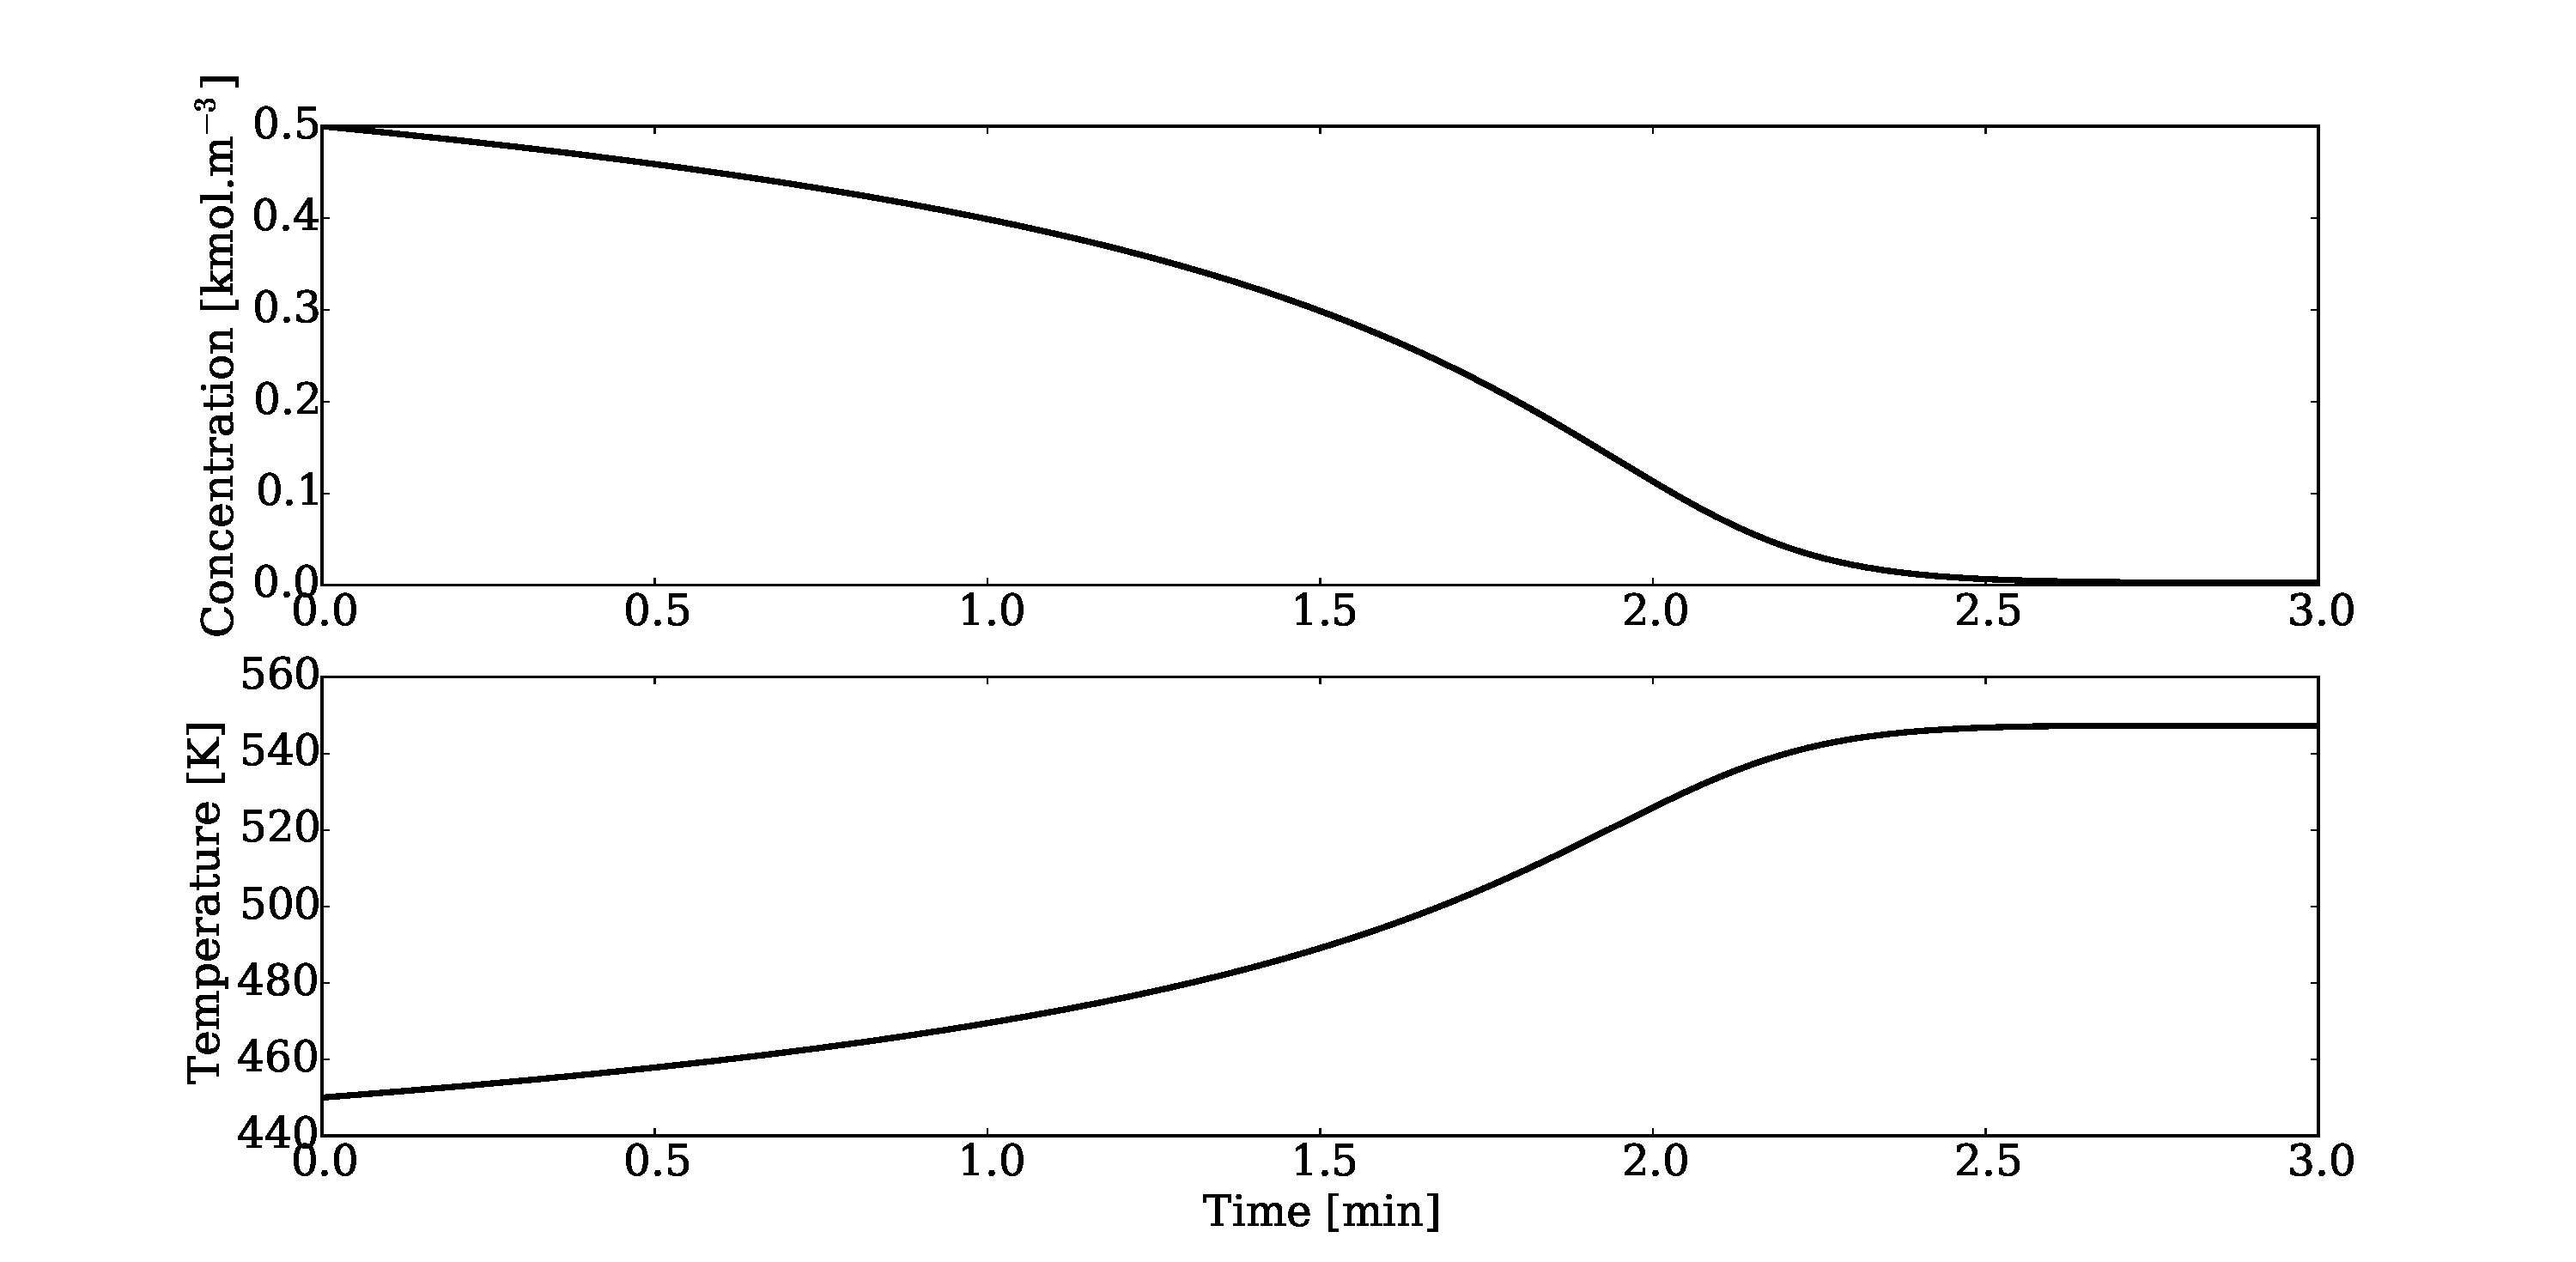
\includegraphics[scale=0.3]{cstr_nl_1.pdf}
\caption{Transient response of the CSTR under nominal operating conditions with initial condition $(0.5, 450)$ and $h=0.001$.}
\label{fig_cstr_nl_1}
\end{figure}
\begin{figure}[H] 
\centering
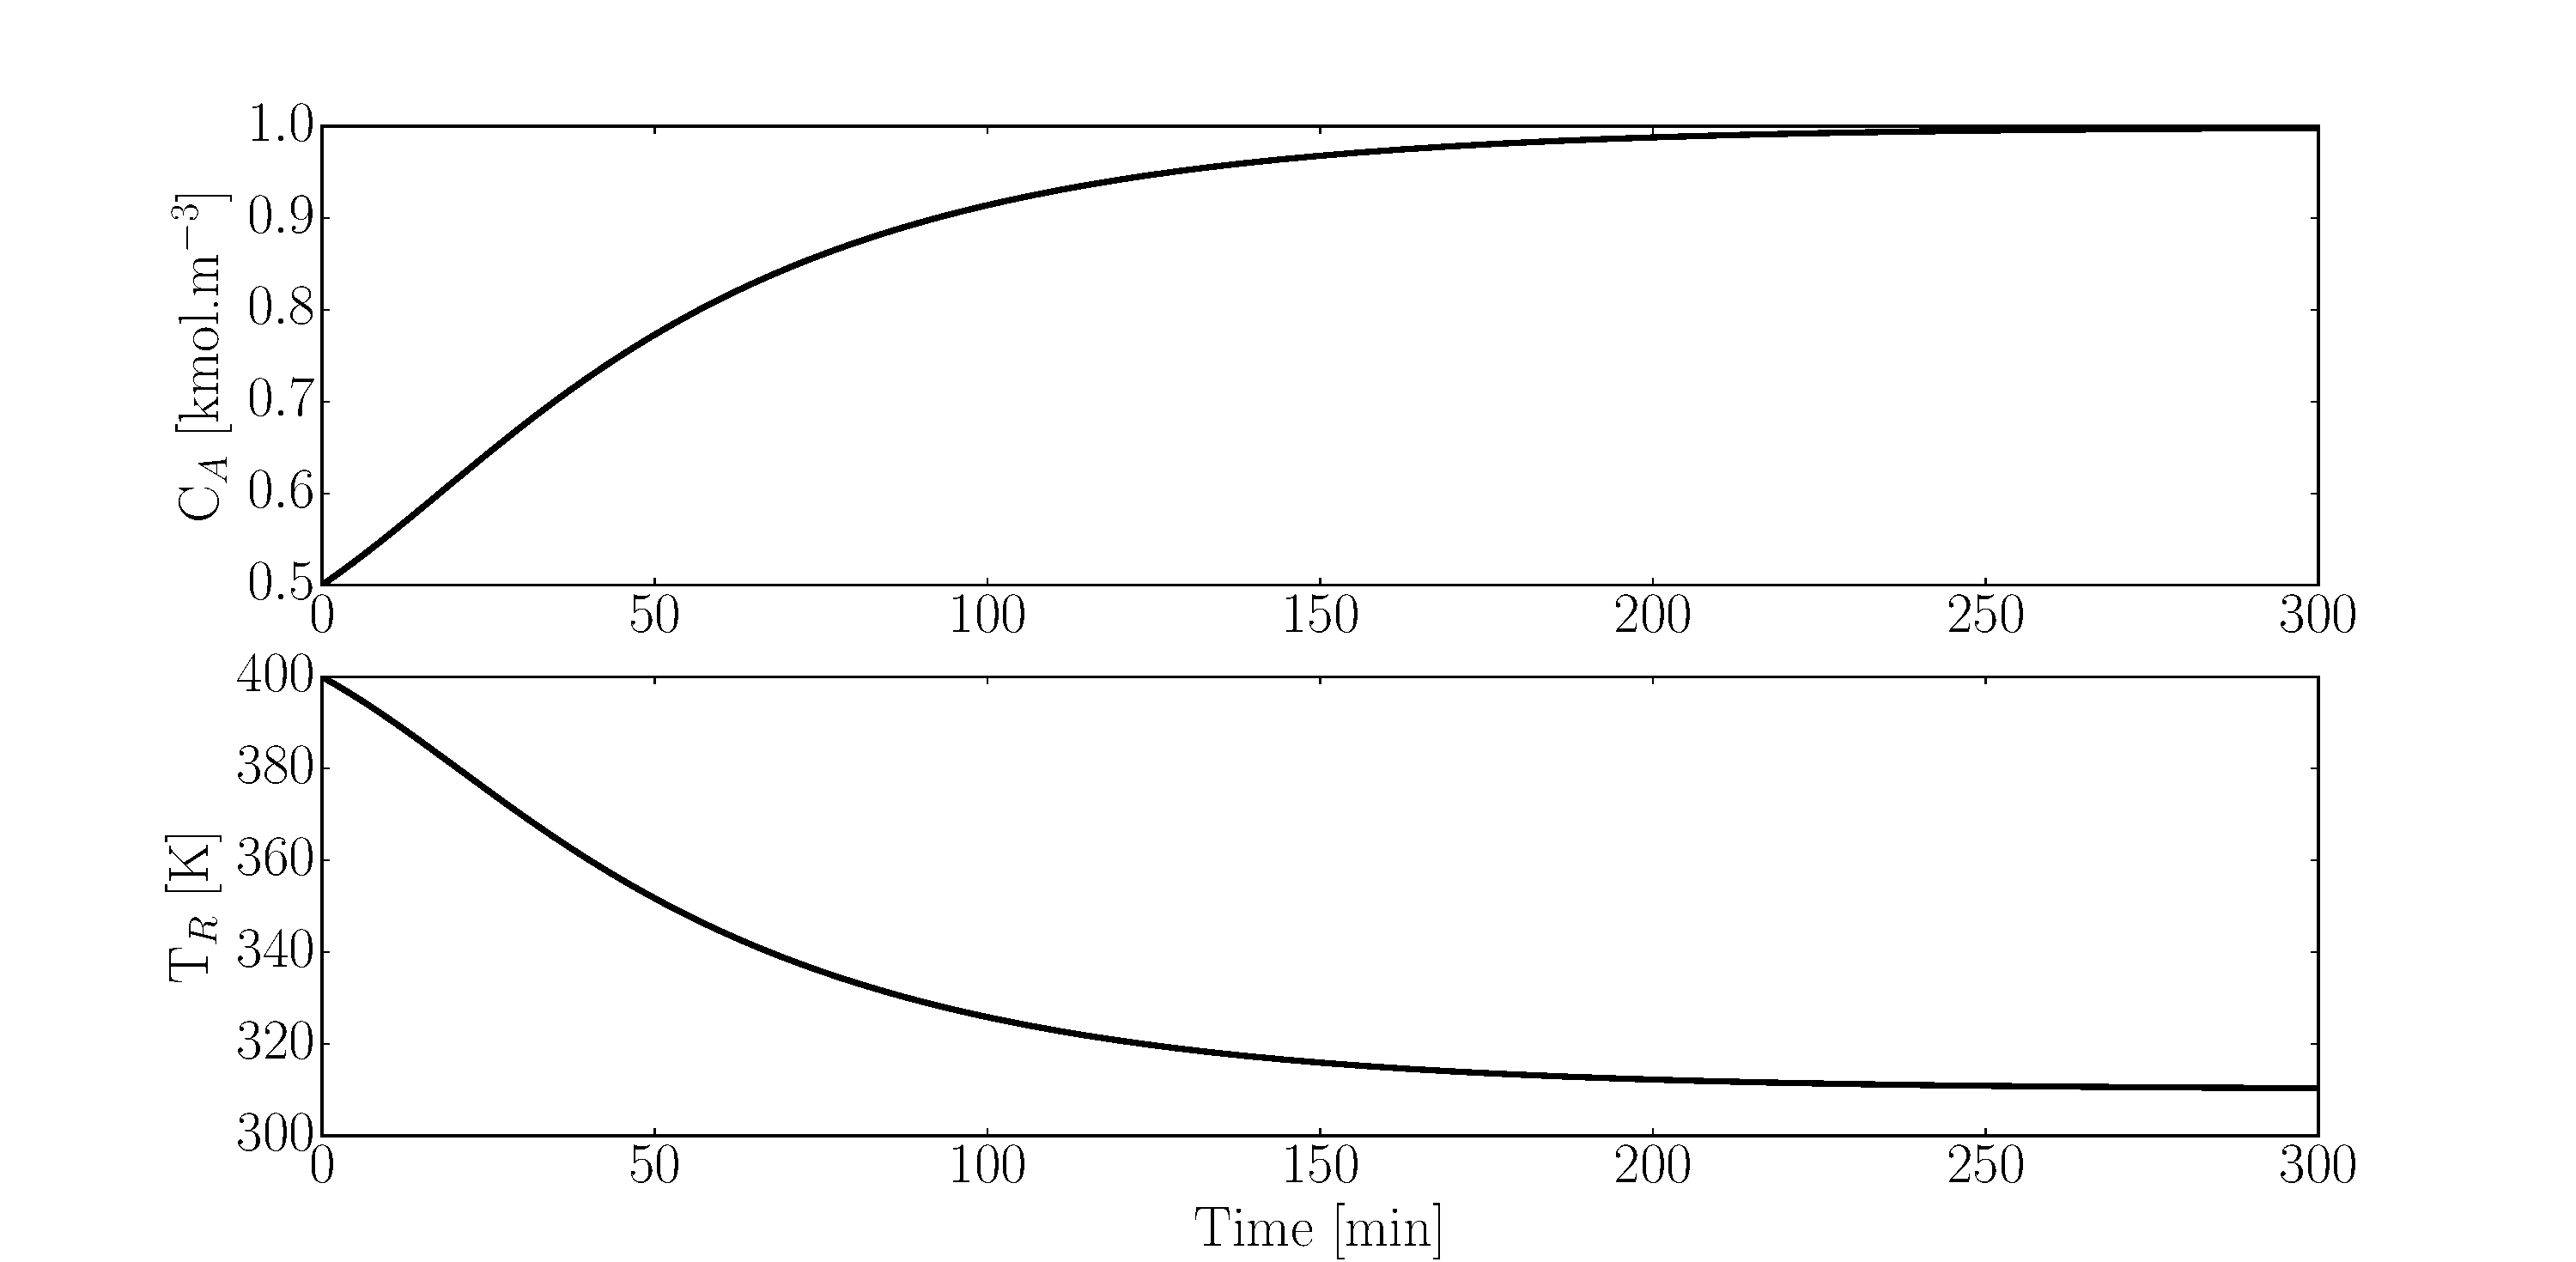
\includegraphics[scale=0.3]{cstr_nl_2.pdf}
\caption{Transient response of the CSTR under nominal operating conditions with initial condition $(0.5, 400)$ and $h=0.001$.}
\label{fig_cstr_nl_2}
\end{figure}
It is often desirable to linearise a nonlinear system about some point, usually the operating point, to simplify the model. Computationally this is advantageous because many control techniques have been designed specifically for linear systems. Practically linearisation is only valid in a small region around the point of linearisation. If the system moves away from the linearisation point the linear approximation can become grossly inaccurate. 

Based on Figure \ref{fig_cstr_nl_1}, where the dynamics are fast, we can venture a guess that linearisation will be a bad approximation, except for a very small time period, of plant behaviour because the states will rapidly move away from the point of linearisation.

On the other hand, based on Figure \ref{fig_cstr_nl_2}, we can venture a guess that linearisation will be a fair approximation of plant behaviour for a meaningful period of time because the dynamics are slow.

\subsection{Linearised Models}
The approach of using piecewise affine (linear) functions for control, based on linearisation around critical points, has been investigated in literature \cite{du}\cite{kvasnica}. Typically the state domain is discretised into regimes and the linear approximation of the model in each regime is used for control. The benefit of this approach is that the non-linear problem  can then be handled by linear methods for which efficient algorithms exist. Drawbacks of this approach are computational complexity \cite{du} and poor control performance because the models are inaccurate.

We will also attempt to use linear models for the purposes of control. First we present a general linearisation technique. Consider an arbitrary point in the state space $(C_A^*, T_R^*)$. Then (\ref{eq_lin}) is the general linearised model around $(C_A^*, T_R^*)$.
\begin{equation}
\begin{pmatrix}
\dot{C_A} \\ \dot{T_R}
\end{pmatrix} = \begin{pmatrix}
f(C_A^*, T_R^*) \\ g(C_A^*, T_R^*)
\end{pmatrix} + J(C_A^*, T_R^*)\begin{pmatrix}
C_A \\ T_R
\end{pmatrix} - J(C_A^*, T_R^*)\begin{pmatrix}
C_A^* \\ T_R^*
\end{pmatrix}
\label{eq_lin}
\end{equation}
It is possible to apply the Runge-Kutta method to (\ref{eq_lin}) and reduce the system, for a given $h$, into the standard linear state space form as shown in (\ref{eq_rkss}). 
\begin{equation}
\begin{pmatrix}
C_A \\ T_R
\end{pmatrix}_{t+1} = A(C_A^*, T_R^*) \begin{pmatrix}
C_A \\ T_R
\end{pmatrix}_{t} + B(C_A^*, T_R^*)Q + b(C_A^*, T_R^*)
\label{eq_rkss}
\end{equation}
Where $Q$ is the heat input to the system and comes from the first term on the right hand side of the equals sign in (\ref{eq_lin}). The algebra is quite involved so we merely state that it is possible and refer the reader to the programmatic implementation for further details: see the function \textit{linearise} in the module \textit{Reactor\_functions} in the folder \textit{CSTR\_Model}.



\bibliographystyle{plain}
\bibliography{research}

\end{document}
\documentclass[../masters.tex]{subfiles}

\begin{document}
\graphicspath{{./imgs/}{../imgs/}} %look for images

\section{Linear Models}
In this section we consider probabilistic graphical models of the form shown in Figure \ref{fig_linmod2}. This model is a generalisation of the graphical model seen in the Hidden Markov Model section. We now assume that the states ($x_1,x_2,...$) and observations ($y_1,y_2,...$) are continuous random variables but the inputs ($u_1,u_2,...$) are deterministic. Models of this form are called Latent Linear Dynamical Systems (the famous Kalman Filter model falls into this category).
\begin{figure}[H] 
\centering
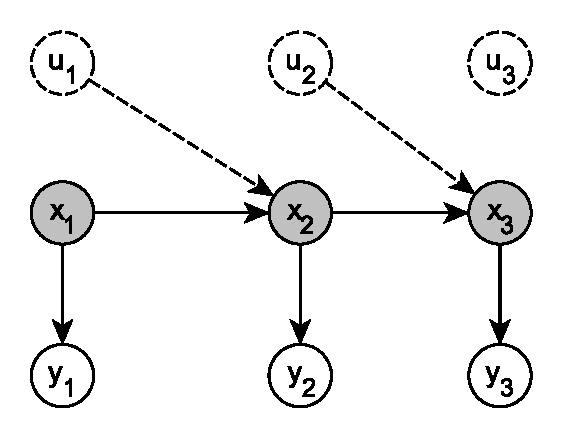
\includegraphics[scale=1.0]{linear_model.pdf}
\caption{Graphical model of this section}
\label{fig_linmod2}
\end{figure}
In the previous section we developed inference algorithms but assumed that the transition and observation functions were discrete. We also noted that this assumption is not appropriate for continuous data. The reason is that one would invariably need to discretise the domain of the continuous random variable under consideration. This would result in intractably large discrete systems if one requires fine resolution. To address this issue we extend the previous model to include both continuous states and observations. 

We assume linearity and that all the random variables are Gaussian. While these are strong assumptions they form the building blocks of much more expressive models as we will discover in the next section. We also assume that the transition and emission functions are time invariant and that the state space model is of the form (\ref{eq_statespace}).
\begin{equation}
\begin{aligned}
x_{t+1} &= Ax_t + Bu_t + w_{t+1} \text{ with } \mathcal{N}(w_{t+1}|0,W) \\
y_{t+1} &= Cx_{t+1} + v_{t+1}  \text{ with } \mathcal{N}(v_{t+1}|0,V)
\end{aligned}
\label{eq_statespace}
\end{equation}
Rewriting the state space model we see that the transition and emission probability density functions are given by (\ref{eq_trans_emiss}). Note that we also assume that the system is first order Markov.
\begin{equation}
\begin{aligned}
p(x_{t+1}|x_t, u_t)&= \mathcal{N}(x_{t+1}|Ax_t+Bu_t, W) \\
p(y_{t+1}|x_t) &= \mathcal{N}(y_{t+1}|Cx_{t+1}, V)
\end{aligned}
\label{eq_trans_emiss}
\end{equation}
We have implicitly assumed that the noise is Gaussian and white\footnote{The noise is temporally independent, has zero mean and finite variance.}. Intuitively one can think of $V$ as the noise associated with state measurements and $W$ being the uncertainty (plant-model mismatch) associated with the linear model of the plant. Additionally, $W$ can also model any unmeasured disturbances which may influence the system\footnote{Note that for the purposes of this dissertation plant is a synonym for the system.}. Thus, larger $V$ and $W$ indicate more uncertainty in the system. 

To fully specify the system we require the transition and emission probability density functions (these implicitly depend on the internal structure of the graphical model in Figure \ref{fig_linmod2}) as well as the prior (initial) distribution of $x_1$.

\subsection{Filtering}
The goal of filtering is to find the posterior distribution $p(x_{t}|y_{1:t}, u_{1:t-1})$. It is pleasing to note that this derivation will follow in an analogous manner to the filtering derivation in the Hidden Markov Model section albeit with continuous Gaussian distributions. The motivation for taking the joint of only the preceding hidden time step is the same as before. 

We start with the prediction expression in (\ref{eq_filter_pred}) and assume, due to the closure of linear conditional Gaussian distributions, that $\alpha(x_{t-1}) = p(x_{t-1}|y_{1:t-1}, u_{1:t-2}) = \mathcal{N}(x_{t-1}|\mu_{t-1}, \Sigma_{t-1}) $. 
\begin{equation}
\begin{aligned}
p(x_t|y_{1:t-1}, u_{1:t-1}) &= \int_{x_{t-1}} p(x_t,x_{t-1}|y_{1:t-1}, u_{1:t-1}) \\
&= \int_{x_{t-1}} p(x_{t-1}|y_{1:t-1}, u_{1:t-1})p(x_{t}|x_{t-1}, y_{1:t-1}, u_{1:t-1}) \\
&= \int_{x_{t-1}} p(x_{t-1}|y_{1:t-1}, u_{1:t-2})p(x_{t}|x_{t-1}, u_{1:t-1}) \\
&= \int_{x_{t-1}} \alpha(x_{t-1})\mathcal{N}(x_{t}|Ax_{t-1}+Bu_{t-1}, W) \\
&= \int_{x_{t-1}} \mathcal{N}(x_{t-1}|\mu_{t-1}, \Sigma_{t-1}) \mathcal{N}(x_{t}|Ax_{t-1}+Bu_{t-1}, W) \\
\end{aligned}
\label{eq_filter_pred}
\end{equation} 
Now we use Bayes' Theorem for Linear Gaussian Models to evaluate the marginal expression as shown in (\ref{eq_filter_pred2}).
\begin{equation}
\begin{aligned}
\int_{x_{t-1}} \mathcal{N}(x_{t-1}|\mu_{t-1}, \Sigma_{t-1}) \mathcal{N}(x_{t}|Ax_{t-1}+Bu_{t-1}, W) &= \mathcal{N}(x_t|A\mu_{t-1}+Bu_{t-1
}, W+ A^T\Sigma_{t-1}A) \\
&= \mathcal{N}(x_t|\mu_{t|t-1},\Sigma_{t|t-1})
\end{aligned}
\label{eq_filter_pred2}
\end{equation}
Intuitively, (\ref{eq_filter_pred2}) is the one step ahead prediction for the hidden state given all the past observations and the past and present inputs. Now we make use of Bayes' Theorem to update our view of $x_t$ given the current observation as shown in (\ref{eq_filter_update}).
\begin{equation}
\begin{aligned}
p(x_t|y_{1:t},u_{1:t-1}) &= p(x_t|y_{t},y_{1:t-1},u_{1:t-1}) \\
&= \frac{p(y_t|x_t,y_{1:t-1},u_{1:t-1})p(x_t|y_{1:t-1},u_{1:t-2}, u_{t-1})}{p(y_t|y_{1:t-1},u_{1:t-1})} \\
&= \frac{p(y_t|x_t)p(x_t|y_{1:t-1},u_{1:t-1})}{p(y_t|y_{1:t-1},u_{1:t-1})} \\
&\propto p(y_t|x_t)p(x_t|y_{1:t-1},u_{1:t-1})\\
&= p(y_t|x_t)\mathcal{N}(x_t|A\mu_{t-1}+Bu_{t-1
}, W+ A^T\Sigma_{t-1}A) \\
&= \mathcal{N}(y_{t}|Cx_{t}, V)\mathcal{N}(x_t|\mu_{t|t-1},\Sigma_{t|t-1})
\end{aligned}
\label{eq_filter_update}
\end{equation}
Now we again make use of Bayes' Theorem for Linear Gaussian Models to evaluate the conditional expression as shown in (\ref{eq_filter_update2}).
\begin{equation}
\begin{aligned}
p(x_t|y_{1:t},u_{1:t-1}) &=\mathcal{N}(y_{t}|Cx_{t}, V)\mathcal{N}(x_t|\mu_{t|t-1},\Sigma_{t|t-1})\\ 
&= \mathcal{N}(x_t|\Gamma(C^TV^{-1}y + \Sigma_{t|t-1}^{-1}\mu_{t|t-1}), \Gamma) \\
&\text{with } \Gamma = (\Sigma_{t|t-1}^{-1}+C^TV^{-1}C)^{-1} 
\end{aligned}
\label{eq_filter_update2}
\end{equation} 
By using the matrix identity $(A+BD^{-1}C)^{-1}=A^{-1}-A^{-1}B(D+CA^{-1}B)^{-1}CA^{-1}$ and defining $K_t = \Sigma_{t|t-1}C^T(C\Sigma_{t|t-1}C^T+V)^{-1}$ we can simplify $\Gamma$ to the recursive posterior covariance estimate shown in (\ref{eq_filter_covar}). Similarly, using the same matrix identity together with $(P^{-1} B^TR^{-1}B)^{-1})^{-1}B^TR^{-1} = PB^T(BPB^T+R^{-1})$ and the definition of $K_t$ we have the posterior mean estimate as shown in (\ref{eq_filter_mean}). Together (\ref{eq_filter_covar}) and (\ref{eq_filter_mean}) are known as the Kalman Filter equations \cite{murphy2}.
\begin{align}
\Sigma_t &= (I-K_tC)\Sigma_{t|t-1} 
\label{eq_filter_covar} \\
\mu_t &= \mu_{t|t-1} + K_t(y_t - C\mu_{t|t-1})
\label{eq_filter_mean}
\end{align}
Note that for the first time step only the update expression is evaluated as the prediction is the prior of $x_1$. 

Intuitively, the Kalman Filter equations use the state space model to predict the new state distribution and then adjust it by a correction factor $K_t(y_t - C\mu_{t|t-1})$. This factor depends on the difference between the actual observation and the predicted observation. The Kalman gain, $K_t$, represents the inferred confidence of the model. If the model is deemed accurate then the predictions make up most of $\mu_t$ but if the model is bad at predicting the observations then the observations play a bigger part in the next mean estimate \cite{bishop}. 

\subsection{Prediction}
The goal of prediction is to find an expression for the distributions $p(x_{t+h}|y_{1:t}, u_{1:t+h-1})$ and $p(y_{t+h}|y_{1:t}, u_{1:t+h-1})$ with $h\geq 1$. Note that these derivations follow in exactly the same way as the prediction derivations did for the Hidden Markov Models. The reason for this is because the graphical models are the same (the deterministic inputs don't change the structure of the underlying random variable network). 

We start the derivation by considering the one step ahead state prediction in (\ref{eq_pred_state}).
\begin{equation}
\begin{aligned}
p(x_{t+1}|y_{1:t}, u_{1:t}) &= \int_{x_t} p(x_{t+1},x_t|y_{1:t}, u_{1:t}) \\
&= \int_{x_t} p(x_t|y_{1:t}, u_{1:t-1}) p(x_{t+1}|x_t,y_{1:t}, u_{1:t}) \\
&= \int_{x_t} p(x_t|y_{1:t}, u_{1:t-1}) p(x_{t+1}|x_t, u_{t}) \\
&= \int_{x_t} \alpha(x_t) p(x_{t+1}|x_t, u_{t}) \\
&= \int_{x_t} \mathcal{N}(x_t|\mu_t, \Sigma_t) \mathcal{N}(x_{t+1}|Ax_t+Bu_t, W) \\
&= \mathcal{N}(x_{t+1}|Ax_t+Bu_t, W+A\Sigma_t A^T) \\
&= \mathcal{N}(x_{t+1}|\mu_{t+1|t}, \Sigma_{t+1|t})
\end{aligned}
\label{eq_pred_state}
\end{equation}
Note that $\mu_t$ and $\Sigma_t$ is the filtered mean and covariance. We have again relied upon Bayes' Theorem for Linear Gaussian Models to evaluate the marginal integral. We now consider the two step ahead state prediction in (\ref{eq_pred_state2}).
\begin{equation}
\begin{aligned}
p(x_{t+2}|y_{1:t}, u_{1:t+1}) &= \int_{x_{t+1}} p(x_{t+2},x_{t+1}|y_{1:t}, u_{1:t+1}) \\
&= \int_{x_{t+1}} p(x_{t+1}|y_{1:t}, u_{1:t}) p(x_{t+2}|x_{t+1},y_{1:t}, u_{1:t+1}) \\
&= \int_{x_{t+1}} p(x_{t+1}|y_{1:t}, u_{1:t}) p(x_{t+2}|x_{t+1}, u_{t+1}) \\
&= \int_{x_t} \mathcal{N}(x_{t+1}|\mu_{t+1|t}, \Sigma_{t+1|t})\mathcal{N}(x_{t+2}|Ax_{t+1}+Bu_{t+1}, W) \\
&= \mathcal{N}(x_{t+2}|A\mu_{t+1|t}+Bu_{t+1}, W+A\Sigma_{t+1|t} A^T) \\
&= \mathcal{N}(x_{t+2}|\mu_{t+2|t}, \Sigma_{t+2|t})
\end{aligned}
\label{eq_pred_state2}
\end{equation}
It is clear that we have derived a recursive algorithm to estimate the $h^{th}$-step ahead state prediction as shown in (\ref{eq_pred_state_recur}).
\begin{equation}
\begin{aligned}
&p(x_{t+h}|y_{1:t}, u_{1:t+h}) = \mathcal{N}(x_{t+h}|\mu_{t+h|t}, \Sigma_{t+h|t}) \\
&\text{with } \mu_{t+h|t} = A\mu_{t+h-1|t}+Bu_{t+h-1} \\
&\text{and } \Sigma_{t+h|t} = W+A\Sigma_{t+h-1|t} A^T \\
&\text{and } \mu_{t+1|t} = A\mu_t+Bu_{t} \\
&\text{and } \Sigma_{t+1|t} = W+A\Sigma_t A^T \\ 
\end{aligned}
\label{eq_pred_state_recur}
\end{equation}
Inspecting (\ref{eq_pred_state_recur}) we see that the predictive distribution is just the forward projection, using the transition function, of the filtered distribution. Note that it is possible for $\Sigma_{t+h|t}$ to become smaller for increasing $h$ (obviously bounded by $Q$ below). For, if the eigenvalues of $A$ are less than one we have that $A\Sigma_{t+h|t}A^T \leq A\Sigma_{t+h-1|t}A^T$.

Next we consider the observation prediction, $p(y_{t+h}|y_{1:t}, u_{1:t+h-1})$. Again consider the one step ahead prediction as shown in (\ref{eq_pred_obs}).
\begin{equation}
\begin{aligned}
p(y_{t+1}|y_{1:t}, u_{1:t}) &= \int_{x_t, x_{t+1}} p(y_{t+1},x_{t+1},x_t|y_{1:t}, u_{1:t}) \\
&= \int_{x_t, x_{t+1}} p(x_t|y_{1:t}, u_{1:t-1})p(y_{t+1},x_{t+1}|x_t, y_{1:t}, u_{1:t}) \\
&= \int_{x_t, x_{t+1}} p(x_t|y_{1:t}, u_{1:t-1}) p(x_{t+1}|x_t, y_{1:t}, u_{1:t})p(y_{t+1}|x_{t+1}, x_t, y_{1:t}, u_{1:t}) \\
&= \int_{x_t, x_{t+1}} \alpha(x_t) p(x_{t+1}|x_t, u_{t}) p(y_{t+1}|x_{t+1}) \\
&= \int_{x_t, x_{t+1}} \mathcal{N}(x_t|\mu_t,\Sigma_t) \mathcal{N}(x_{t+1}|Ax_t+Bu_t, W) \mathcal{N}(y_{t+1}|Cx_{t+1}, V) \\
&= \mathcal{N}(y_{t+1}|C\mu_{t+1|t}, V+C\Sigma_{t+1|t}C^T)
\end{aligned}
\label{eq_pred_obs}
\end{equation}
We have again used Bayes' Theorem for Linear Gaussian Models and used the nomenclature of the one step ahead state prediction derivation. For the sake of brevity we trust that the reader will see the similarity between the two derivations and allow us to conclude, without proof, that the $h^{th}$-step ahead observation prediction is given by (\ref{eq_pred_obs_recur}).
\begin{equation}
\begin{aligned}
&p(y_{t+h}|y_{1:t}, u_{1:t+h-1}) = \mathcal{N}(y_{t+h}|C\mu_{t+h|t}, R+C\Sigma_{t+h|t}C^T) \\
\end{aligned}
\label{eq_pred_obs_recur}
\end{equation}
It is reassuring to note that the observation prediction is just the state prediction transformed by the observation function.

\subsection{Smoothing and Viterbi Decoding}
For the sake of completeness we state the Kalman Smoothing equations and briefly discuss Viterbi Decoding within the context of conditional linear Gaussian systems. 

The reason we do not go into detail with the smoothing algorithm is because it follows much the same structure as the Hidden Markov Model smoothing algorithm except that we again make use of Bayes' Theorem for Linear Gaussian Models. We are also primarily only interested in filtering and prediction because they are important for the purposes of control which is the focus of this dissertation.

The smoothing algorithm, also called the Rauch, Tung and Striebel (RTS) algorithm for $p(x_t|y_{1:T},u_{1:T-1})$ is also a Gaussian distribution of the form $\mathcal{N}(\hat{\mu}_t, \hat{\Sigma}_t)$. The recursion expressions for the posterior mean and covariance are shown in (\ref{eq_smooth2}).
\begin{equation}
\begin{aligned}
&\hat{\mu}_t = \mu_t + J_t\left(\hat{\mu}_{t+1}-(A\mu_t+Bu_{t-1})\right) \\
&\hat{\Sigma}_t = \Sigma_t + J_t(\hat{\Sigma}_{t+1}-P_t)J^T_t \\
&\text{with } P_t = A\Sigma_tA^T + W \\
&\text{and } J_t = \Sigma_t A^T (P_t)^{-1}\\
&\text{and } \hat{\mu}_T = \mu_T\\
&\text{and } \hat{\Sigma}_T = \Sigma_T
\end{aligned}
\label{eq_smooth2}
\end{equation}

Finally, we know from the Chain Rule for Bayesian Networks and Figure \ref{fig_linmod2} that the joint distribution for $p(x_{1:T},y_{1:T}, u_{1:T-1}) = p(x_1)p(y_1|x_1)\Pi^T_{t=2} p(y_t|x_t)p(x_{t}|x_{t-1},u_{t-1})$. Since Gaussian distributions are closed under multiplication this joint distribution is also a Gaussian distribution. It can be shown that maximising with respect to all latent variables jointly or maximising with respect to the marginal distributions of the latent variables is the same because the mean and the mode of a Gaussian distribution coincide \cite{barber}.

\subsection{Filtering the CSTR}
In this section we apply the Kalman Filter to the CSTR introduced earlier. We use the linear model around the unstable operating point $(C_A^2, T_R^2)$ as shown in (\ref{eq_linmodel}). Note that the matrix $A$ and vectors $B, b$ depend on the step size and should be recalculated for different $h$. To make things concrete we have used $h=0.1$ here. Note that we only measure temperature for now.
\begin{equation}
\begin{aligned}
A &= \begin{pmatrix}
0.9959 & -6.0308\times 10^{-5} \\
0.4186 & 1.0100
\end{pmatrix} \\
B &= \begin{pmatrix}
0 \\ 8.4102\times 10^{-6}
\end{pmatrix} \\
C &= \begin{pmatrix}
0 & 1
\end{pmatrix} \\
W &= \begin{pmatrix}
1\times 10^{-5} & 0 \\ 0 & 4
\end{pmatrix} \\
V &= \begin{pmatrix}
10
\end{pmatrix}
\end{aligned}
\label{eq_linmodel}
\end{equation}
The system noise $W$ indicates that the standard deviation of the concentration component of the model is 0.001 kmol/m$^{-3}$ and the temperature component is 2 K. This indicates that we are quite uncertain about the accuracy of the linear model. The measurement noise implies that 68\% of the measurements will fall between $\pm\sqrt{10}$ of the actual state. We use a vague initial state with mean at the initial condition and covariance $W$.

In Figure \ref{fig_kftimeseries} we illustrate the strengths and weaknesses of the Kalman Filter. Since we derived the recursion equations analytically it is computationally efficient to use, the biggest cost is a matrix inversion which needs to be computed at each time step. During the initial part of the simulation the filter very accurately estimates the current system states because the model is accurate in this region. Thus the filter is able to infer the true state in the presence of noisy measurements. 

Unfortunately the recursion equations assumed the system can be described by a linear model. With time the trajectories move away from the linearisation point (because the linearisation point is unstable) and thus the linear model becomes less accurate. This has a detrimental effect on the quality of the Kalman filter estimate as the filter effectively starts to solely rely on the measurements to infer the states. This works reasonably well for the measured states ($T_R$), but since we do not measure concentration the filter is forced to incorporate the linear model prediction which is grossly inaccurate. 
\begin{figure}[H] 
\centering
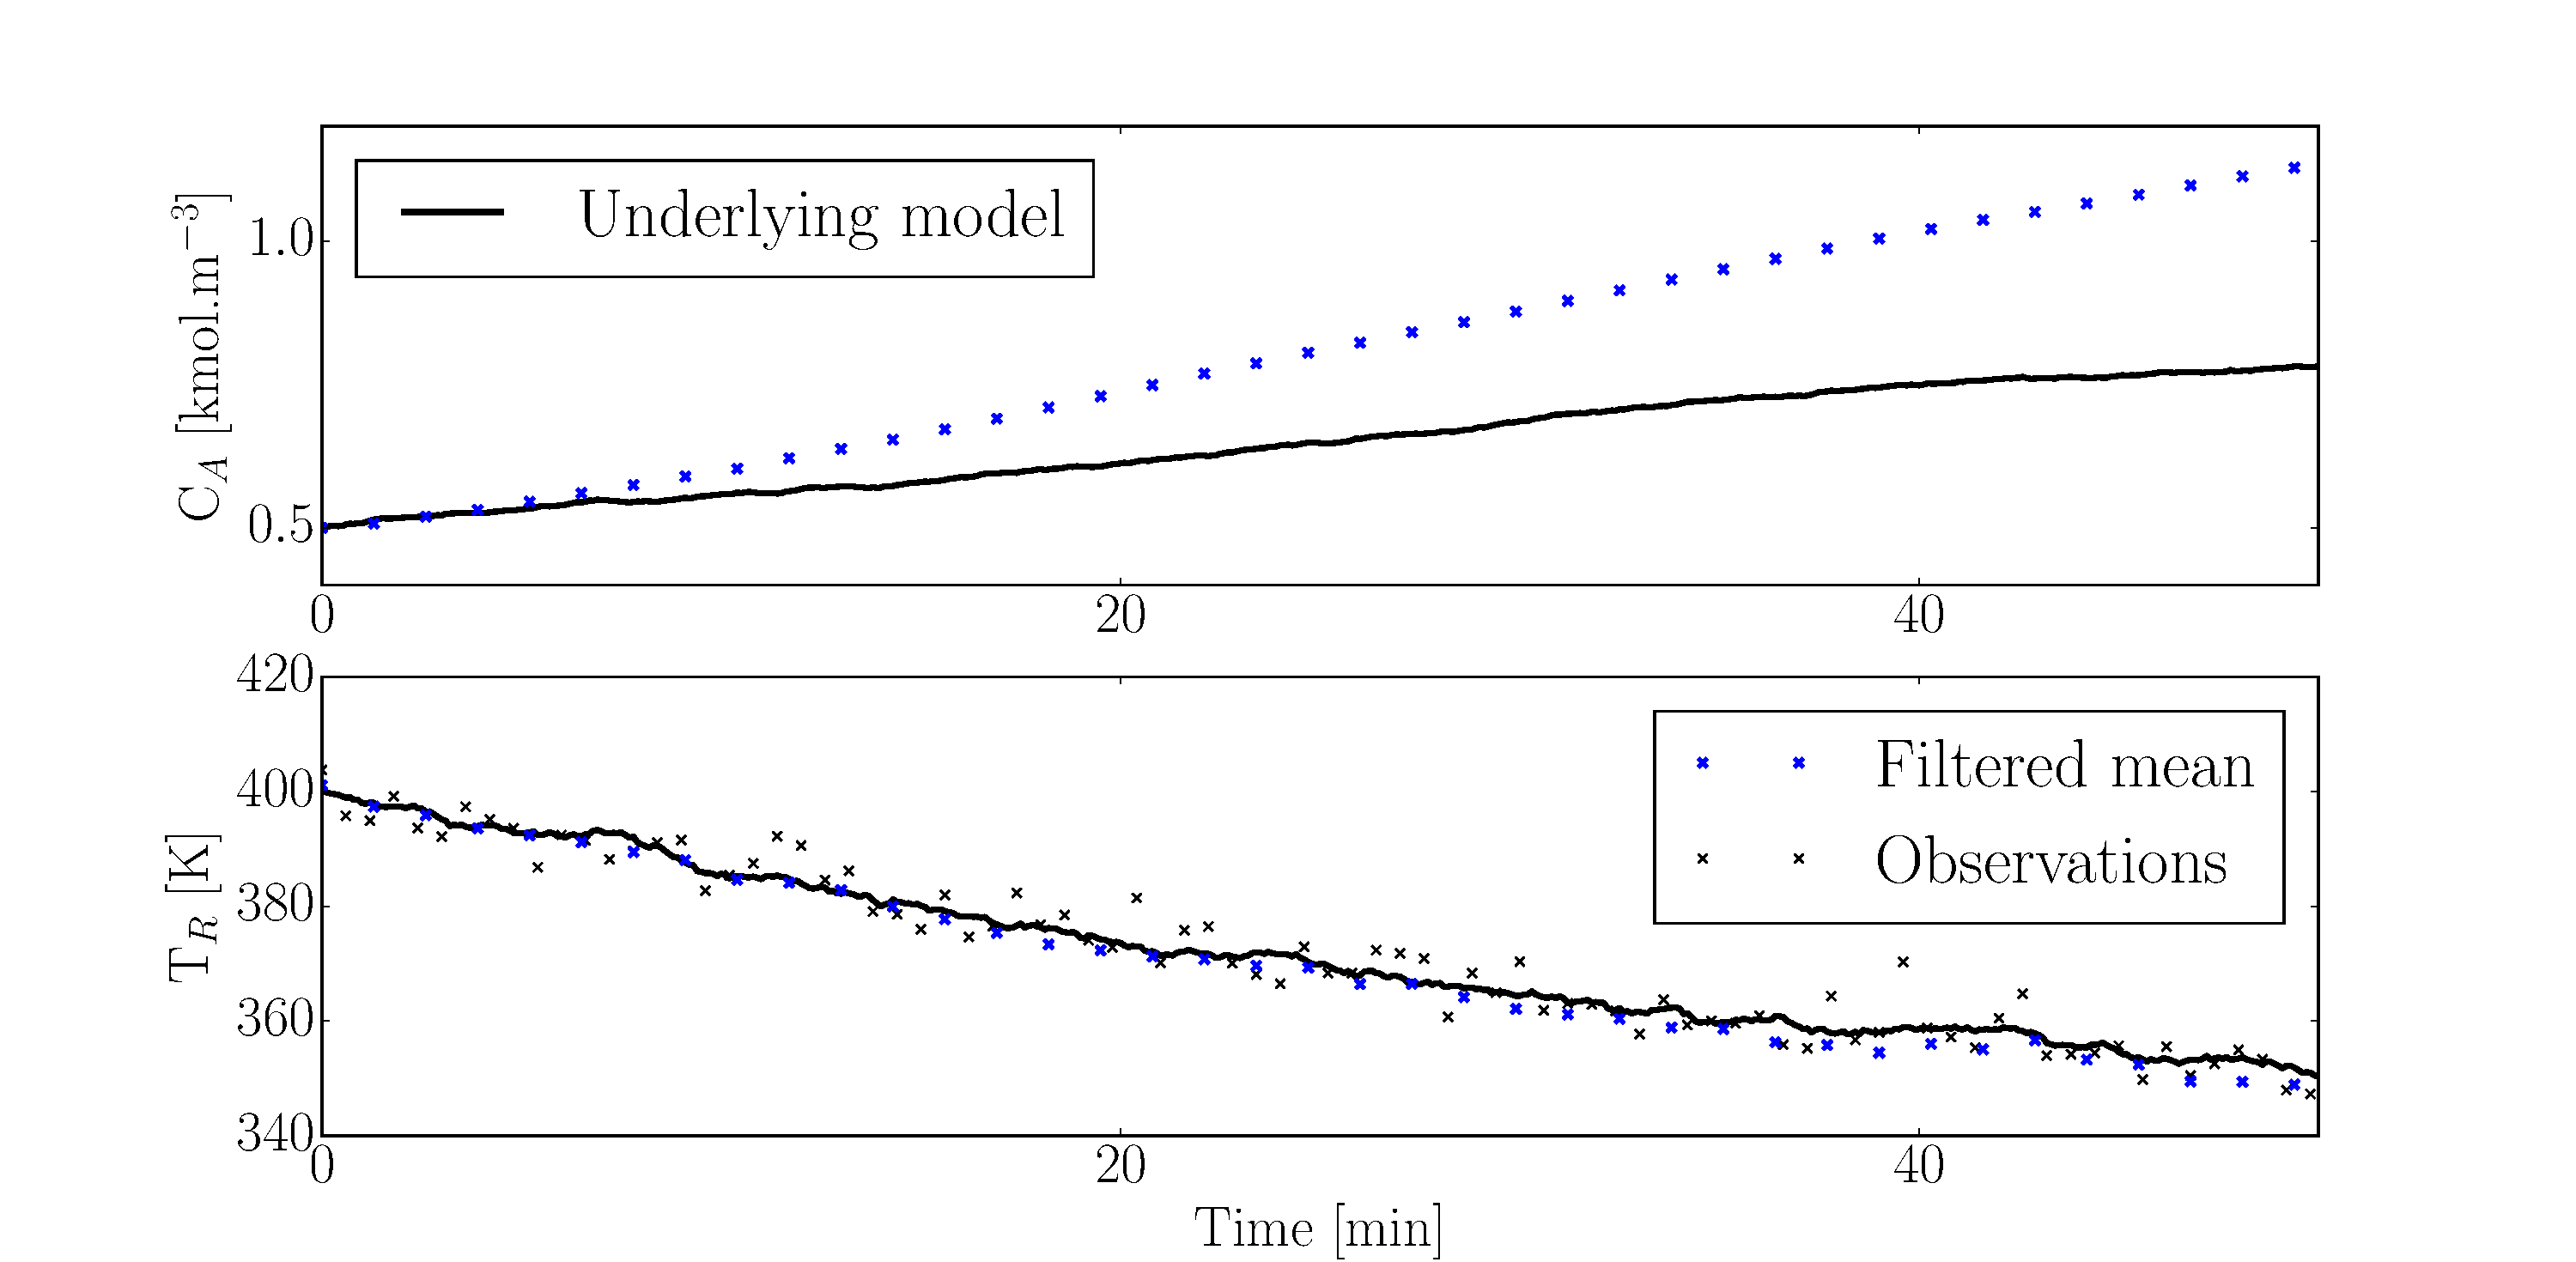
\includegraphics[scale=0.30]{kalman_filter_timeseries_M1.pdf}
\caption{Kalman Filter superimposed on the time series evolution of the CSTR with initial condition $(0.50, 400)$ and measuring only temperature.}
\label{fig_kftimeseries}
\end{figure}
In Figure \ref{fig_kfphase} we see another interesting property of Kalman Filters. The posterior covariance quickly converges to a constant value (the error ellipses quickly stop changing shape) which is independent of the observations. This is a general property of linear Gaussian systems \cite{barber} and is evident from the recursion expression. The modelled system dynamics and noise are the only factors affecting the covariance. If the model is accurate this is not a problem but we see that as the model becomes less accurate the filter maintains the same level of confidence in its estimate. This is quite undesirable behaviour because the confidence in the estimate is not a function of the observations. 

It is also interesting to consider the shape of the error ellipses. Notice how they are short vertically - indicating less uncertainty in the temperature state dimension but wide horizontally - indicating more uncertainty in the concentration state dimension. Intuitively this is plausible because, since we do not measure concentration, we are less sure about the underlying state. 

In Figure \ref{fig_kfphase} we see that while the temperature estimate is still trustworthy (the black crosses line up horizontally with the red crosses) the concentration estimate diverges.
\begin{figure}[H] 
\centering
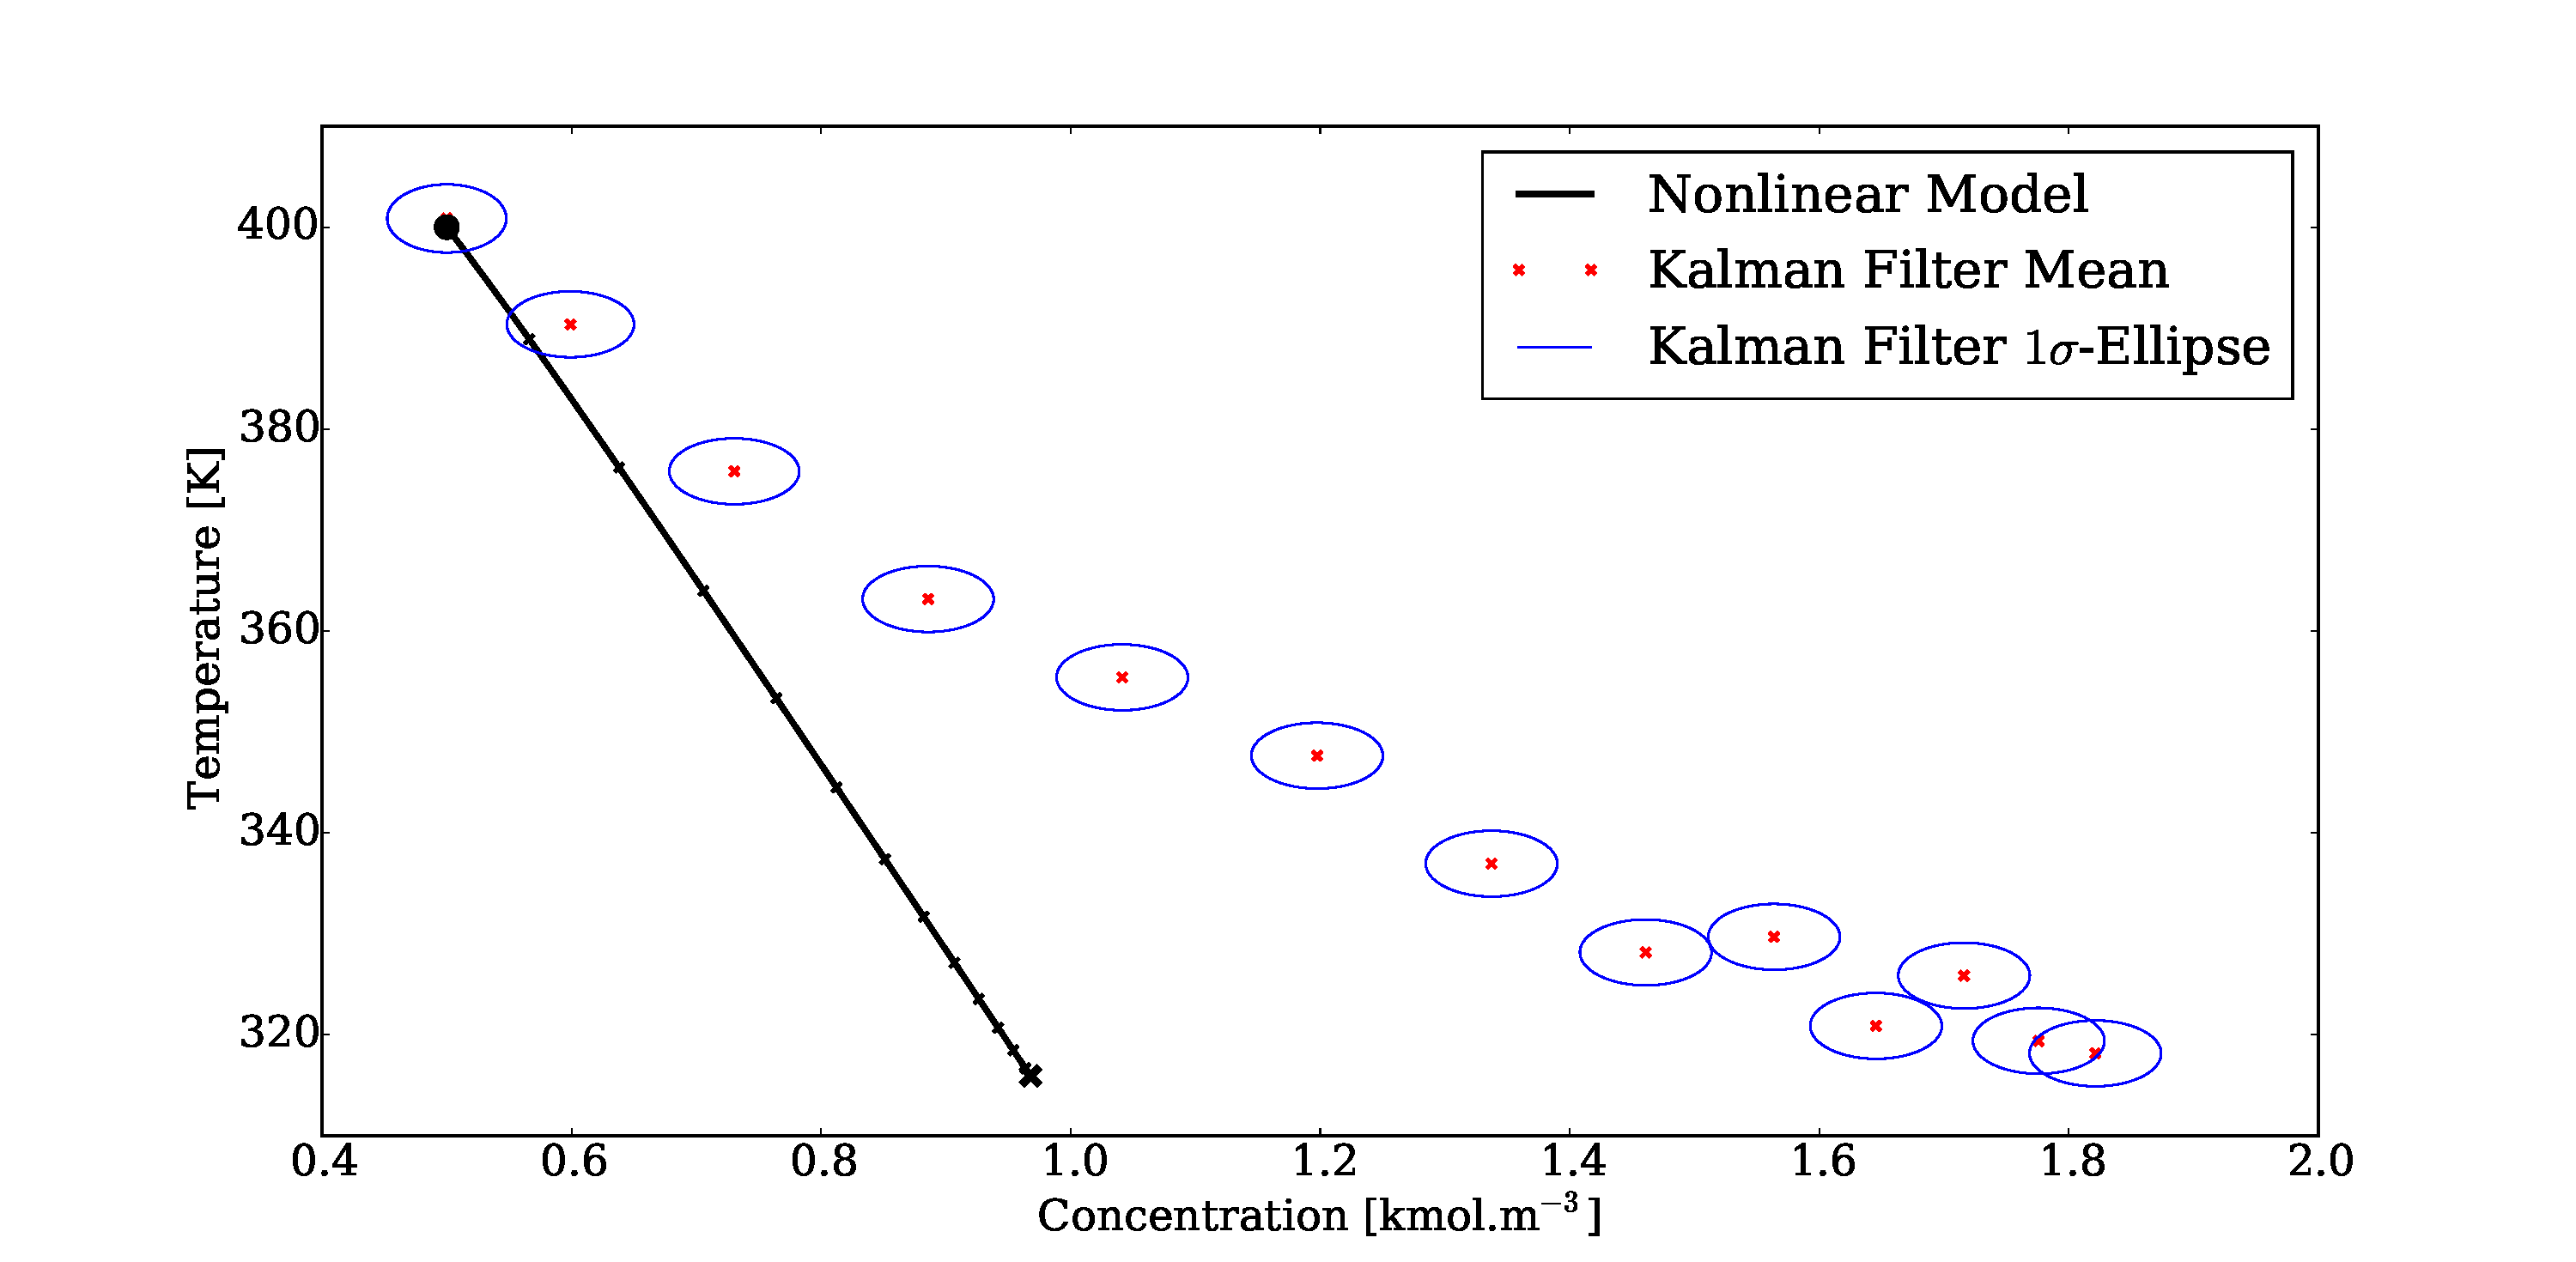
\includegraphics[scale=0.30]{kalman_filter_phase_M1.pdf}
\caption{Phase plane of the hidden states of the CSTR with mean and one-sigma ellipses superimposed thereupon. Only temperature is measured.}
\label{fig_kfphase}
\end{figure}
The root of the problem lies in the unsuitability of the model rather than our inference technique. It can be shown that for linear systems with Gaussian noise the Kalman Filter is the optimal state estimator \cite{shalom}. 

Based on our discussion where the CSTR example was introduced we know that the linear models will not always be very accurate. We therefore modify (\ref{eq_linmodel}) to also incorporate concentration measurements. In this case we have that $C = \begin{pmatrix}
1 & 0\\0 &1
\end{pmatrix}$ and $V = \begin{pmatrix}
1\times 10^{-3} & 0\\0 & 10
\end{pmatrix}$ with everything else the same. The time evolution of the states is shown in Figure \ref{fig_kftime2} and the state space representation is shown in Figure \ref{fig_kfphase2}. 
\begin{figure}[H] 
\centering
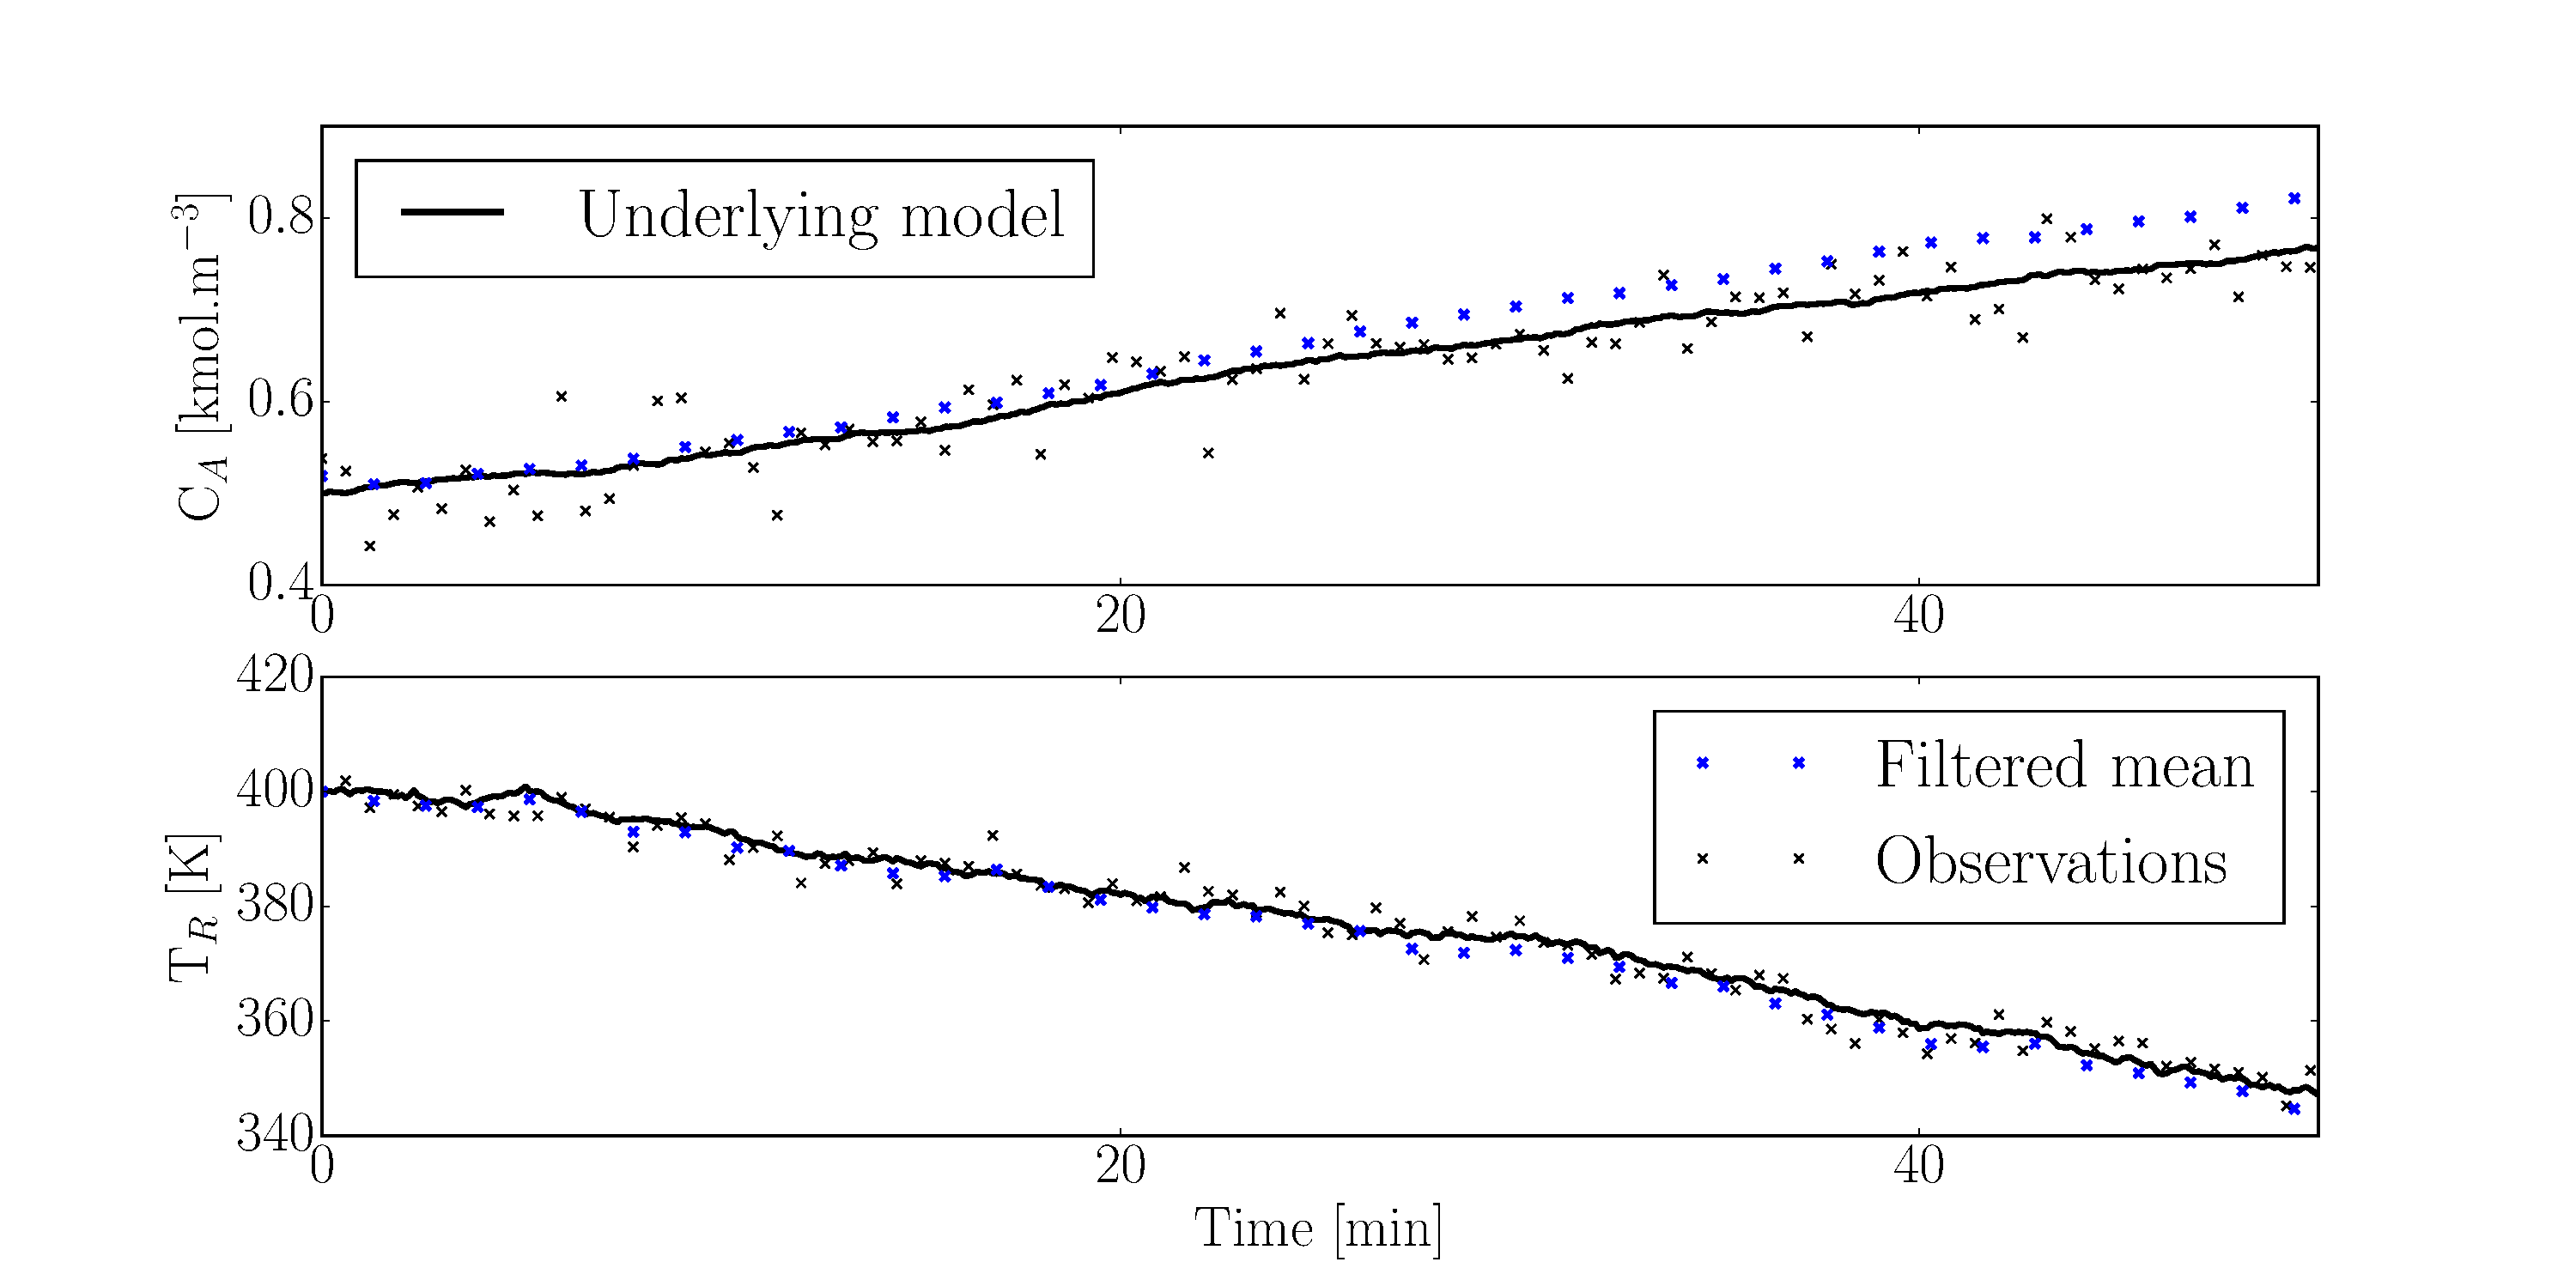
\includegraphics[scale=0.30]{kalman_filter_timeseries_M2.pdf}
\caption{Kalman Filter superimposed on the time series evolution of the CSTR with initial condition $(0.50, 400)$ and measuring both temperature and concentration.}
\label{fig_kftime2}
\end{figure}
\begin{figure}[H] 
\centering
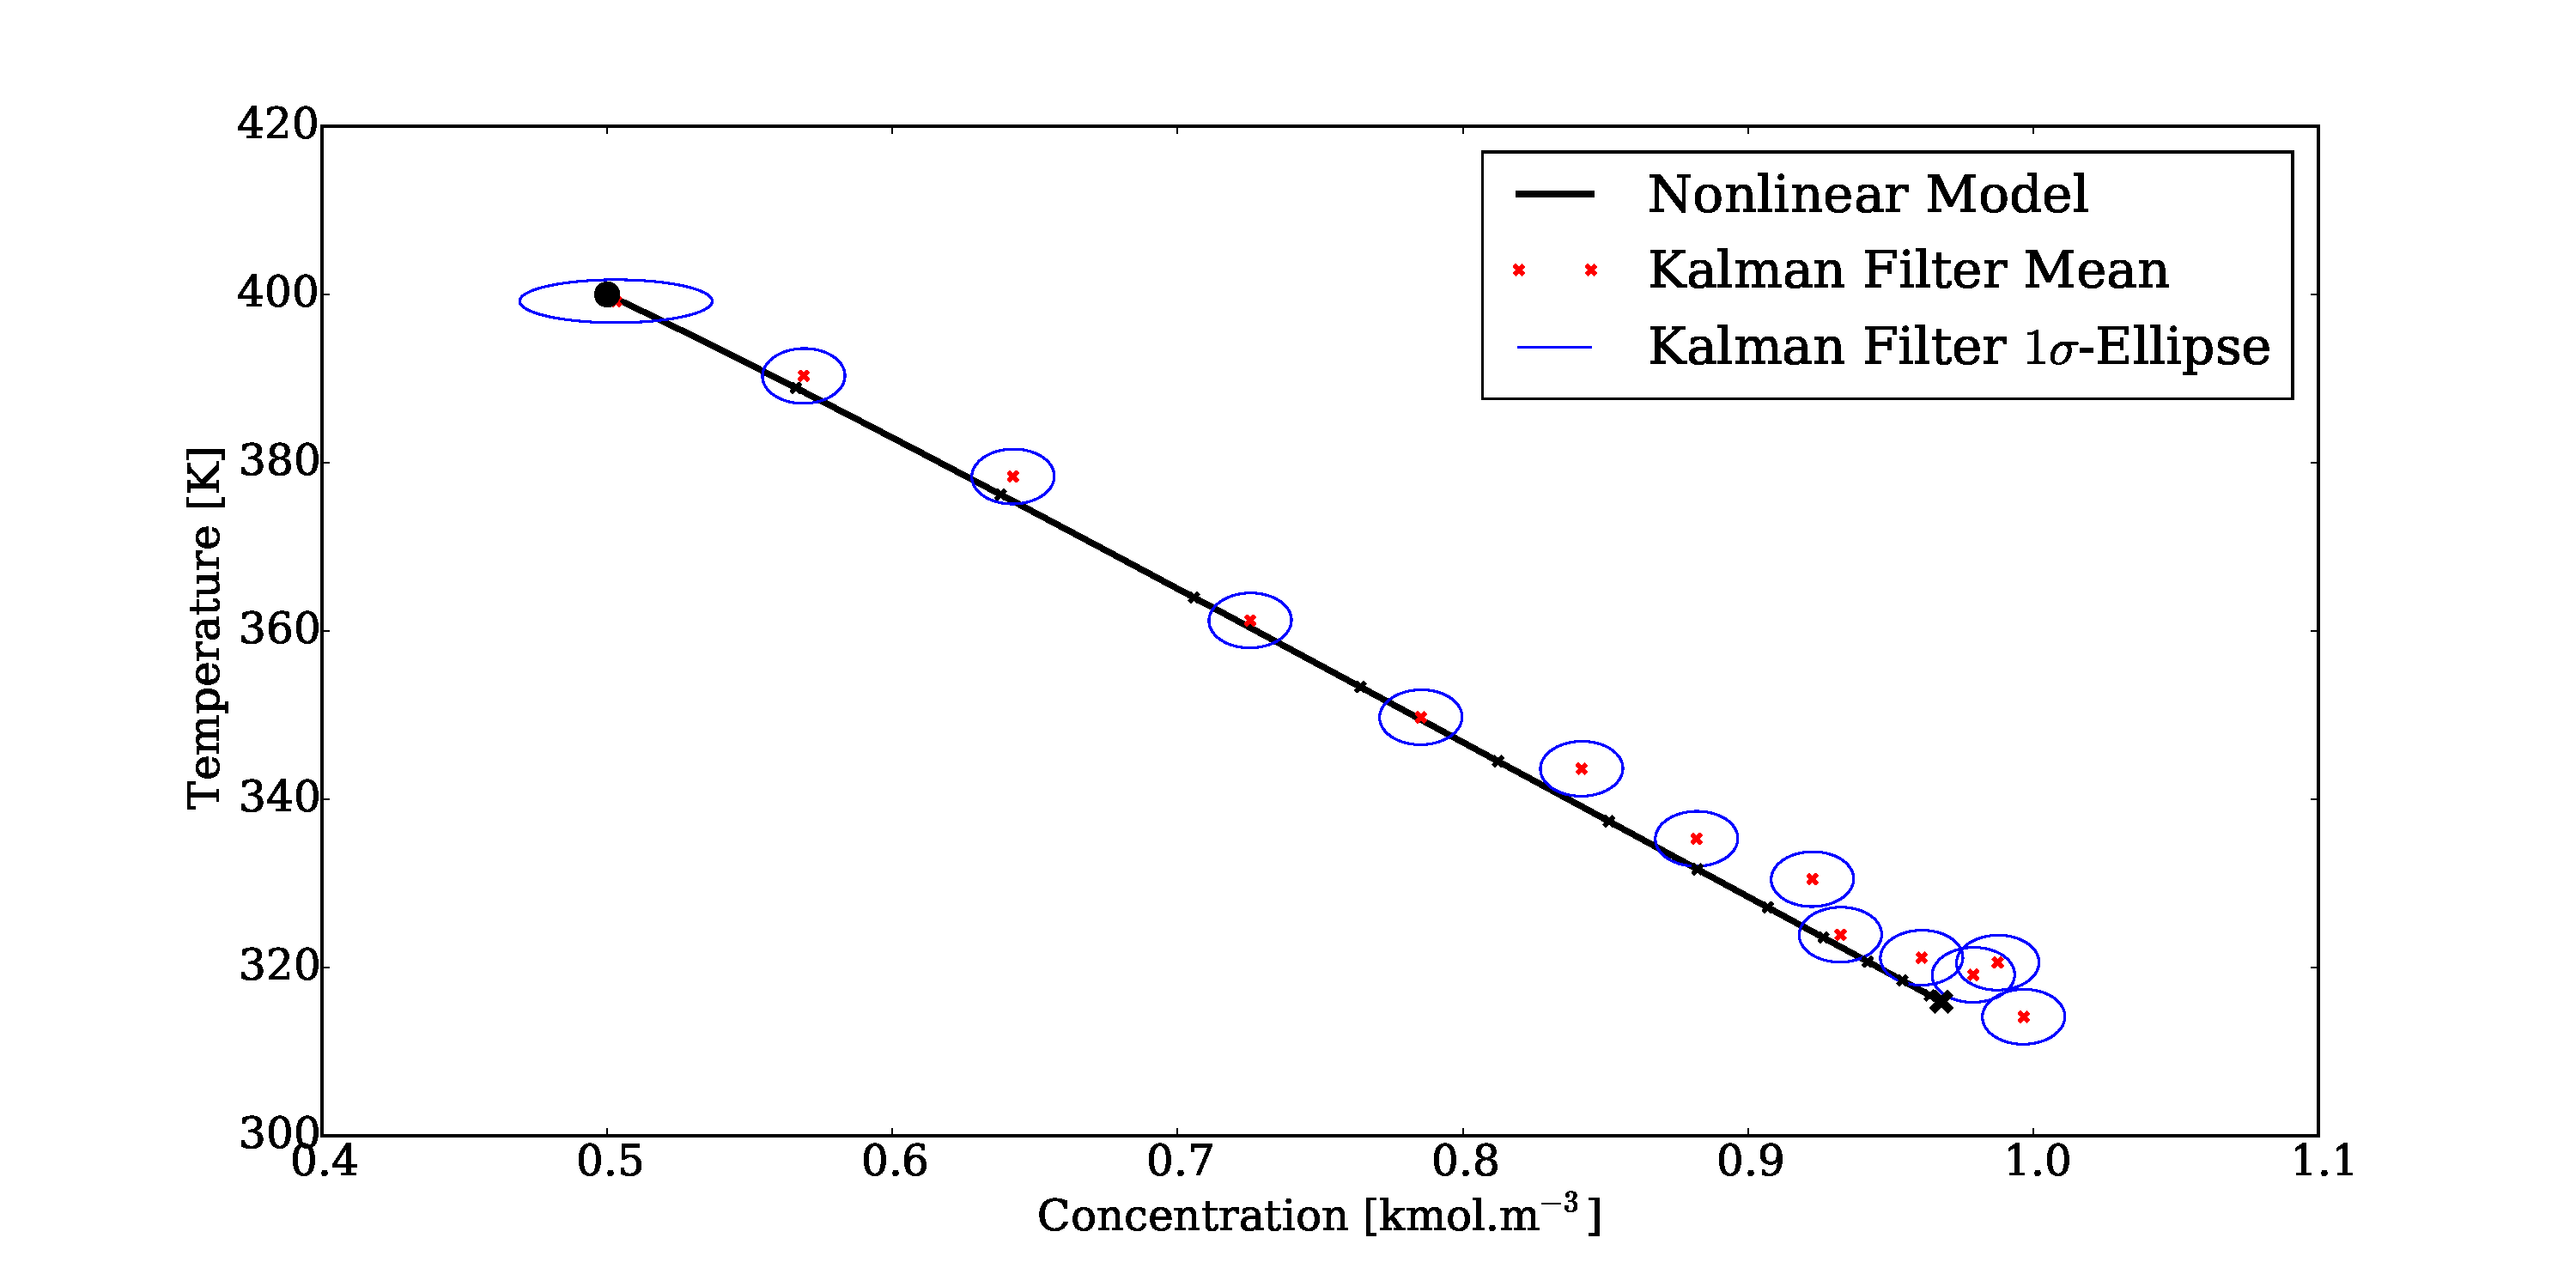
\includegraphics[scale=0.30]{kalman_filter_phase_M2.pdf}
\caption{State space diagram of the CSTR with mean and one-sigma ellipses superimposed thereupon. Both concentration and temperature are measured.}
\label{fig_kfphase2}
\end{figure}
Comparing Figures \ref{fig_kfphase} and \ref{fig_kfphase2} we see that by incorporating the state measurement the state estimation is much more accurate. It is not necessary to directly measure concentration as we have done: any measurement which depends on $C_A$ (or even both $C_A$ and $T_R$) would suffice. The second measurement reduces our uncertainty in the concentration state estimate because we have more to base our inference on than just a bad model.  

\subsection{Controlling the CSTR}

\bibliographystyle{plain}
\bibliography{research}

\end{document}
\chapter{Inference using Nonlinear Models}
\label{sec_inf_nonlin_mods}
In this section we consider probabilistic Graphical Models of the form shown in Figure \ref{fig_nlmod}. These models have exactly the same form as the models in Section \ref{sec_inf_lin_mods}. The variables retain their meaning as before but we generalise the model by dropping the linearity assumption. Unfortunately, this generalisation, although allowing us to expand our investigation to a much more expressive class of models, makes closed form solutions to the inference problem intractable in general.   
\begin{figure}[H] 
\centering
\begin{tikzpicture}

  % Define nodes
  \node[obs] (ya) {$y_0$};
  \node[obs, right=of ya] (yb) {$y_1$};
  \node[obs, right=of yb] (yc) {$y_2$};
  \node[latent, above=of ya]  (xa) {$x_0$};
  \node[latent, above=of yb, right=of xa]  (xb) {$x_1$};
  \node[latent, above=of yc, right=of xb]  (xc) {$x_2$};
  \node[det, above=of xa] (da) {$u_0$};
  \node[det, above=of xb] (db) {$u_1$};
  
  % Connect the nodes
  \edge {da} {xb};
  \edge {db} {xc};
  \edge {xa} {ya};
  \edge {xb} {yb};
  \edge {xc} {yc};
  \edge {xa} {xb};
  \edge {xb} {xc};
  
\end{tikzpicture}
\caption{Graphical model of this section}
\label{fig_nlmod}
\end{figure}
We again assume that the transition and emission functions are time invariant. The state space model is now of the form (\ref{eq_nlstatespace}).
\begin{equation}
\begin{aligned}
x_{t+1} &= f(x_t, u_t, w_{t+1}) \\
y_{t+1} &= g(x_{t+1}, v_{t+1})
\end{aligned}
\label{eq_nlstatespace}
\end{equation}
Note that we make no assumption about the functional form of the noise terms $w_t,v_t$. In practice it is customary to assume that they have zero mean but otherwise are not restricted. Additionally, to simplify notation we will omit the dependence on $u$ of $f$ and $g$ and their associated distributions. Since $u$ is a deterministic variable, by assumption, it is straightforward to incorporate it into later analysis. 

\section{Sequential Monte Carlo Methods}
\label{sec_asir}
Many approximate inference techniques exist in literature, the most notable ones include Gaussian Sum Filters \cite{gsf1} and Particle based methods. We shall focus only on Sequential Monte Carlo (SMC) methods, of which Particle based methods are a subset, because it is simple to implement and generalises well (and easily) to more complex graphical models. 

SMC methods are a general class of Monte Carlo methods which sample sequentially from the growing target distribution $\pi_t(x_{0:t})$. By only requiring that $\gamma_t$ be known point-wise we have the framework of SMC methods as shown in (\ref{eq_SMC1}). Note that $Z_t$ is some normalisation constant \cite{pftut}.
\begin{equation}
\begin{aligned}
\pi_t(x_{0:t}) &= \frac{\gamma_t(x_{0:t})}{Z_t} \\
Z_t &= \int_{x_{0:t}} \gamma_t(x_{0:t})
\end{aligned}
\label{eq_SMC1}
\end{equation} 
For example, in the context of filtering we have that $\gamma_t(x_{0:t}) = p(x_{0:t},y_{0:t})$ and $Z_t = p(y_{0:t})$ so that $\pi_t(x_{0:t}) = p(x_{0:t}|y_{0:t})$. 

It is possible to approximate the distribution $\pi_t(x_{0:t})$ by drawing $N$ samples $X_{0:t}^i \backsim \pi_t(x_{0:t})$ and using the Monte Carlo method to find the approximation $\hat{\pi}_t(x_{0:t})$ as shown in (\ref{eq_SMC2}).
\begin{equation}
\hat{\pi}_t(x_{0:t}) = \frac{1}{N}\sum_{i=1}^N \delta(X^i_{0:t}, x_{0:t})
\label{eq_SMC2}
\end{equation}
We denote the Dirac Delta function of $x$ with mass located at $x_0$ by $\delta(x_0,x)$. It is easy to approximate the marginal $\pi_t(x_{t})$ as shown in (\ref{eq_SMC3}).
\begin{equation}
\hat{\pi}_t(x_{t}) = \frac{1}{N}\sum_{i=1}^N \delta(X^i_{t}, x_{t})
\label{eq_SMC3}
\end{equation}
It can be shown that the variance of the approximation error of $\pi_t$ decreases at rate $\mathcal{O}(\frac{1}{N})$. Unfortunately there are two significant drawbacks to the Monte Carlo approximation. The first is that often we cannot sample from $\pi_t(x_{0:t})$ directly and the second is that even if we could it is often computationally prohibitive. 

We use the Importance Sampling method to address the first problem. We do this by introducing an importance (sometimes called proposal) density $q_t(x_{0:t})$ such that $\pi_t(x_{0:t}) > 0 \implies q_t(x_{0:t}) > 0$. By substituting this into the SMC framework (\ref{eq_SMC1}) we have (\ref{eq_SMC4}).
\begin{equation}
\begin{aligned}
\pi_t(x_{0:t}) &= \frac{w_t(x_{0:t})q_t(x_{0:t})}{Z_t} \\
Z_t &= \int_{x_{0:t}} w_t(x_{0:t})q_t(x_{0:t})
\end{aligned}
\label{eq_SMC4}
\end{equation} 
Where we have defined the unnormalised weight function $w_t(x_{0:t}) = \frac{\gamma_t(x_{0:t})}{q_t(x_{0:t})}$. It is possible, for example, to set $q_t$ to a multivariate Gaussian which is easy to sample from. By drawing $N$ samples $X_{0:t}^i \backsim q_t(x_{0:t})$ and using (\ref{eq_SMC4}) we have (\ref{eq_SMC5}). 
\begin{equation}
\begin{aligned}
\hat{\pi}_t(x_{0:t}) &= \frac{1}{N}\sum_{i=1}^N W_t^i\delta(X^i_{0:t}, x_{0:t}) \\
\hat{Z}_t &= \frac{1}{N}\sum_{i=1}^N w_t(X^i_{0:t}) \\
W^i_t &= \frac{w_t(X^i_{0:t})}{\sum_{i=1}^N w_t(X^i_{0:t})}
\end{aligned}
\label{eq_SMC5}
\end{equation}
Now we will attempt to modify the Importance Sampling method to address the second problem of computational cost incurred by the sampling routine. 

We do this by selecting an importance/proposal distribution which factorises according to $q_t(x_{0:t}) = q_{t-1}(x_{0:t-1})q_t(x_{t}|x_{0:t-1}) = q_0(x_0) \Pi_{k=1}^t q_k(x_k|x_{0:k-1})$. In this way we only need to sample sequentially at each time step: at time $t=0$ we sample $X_0^i \backsim q_0(x_0)$, at time $t=1$ we sample $X_{1}^i \backsim q_1(x_1|x_0)$ and so we build up $X^i_{0:t} \backsim q_t(x_{0:t})$ factor by factor.

The weights can be written in the form (\ref{eq_SMC6}).
\begin{equation}
\begin{aligned}
w_t(x_{0:t}) &= \frac{\gamma_t(x_{0:t})}{q_t(x_{0:t})} \\
&= \frac{\gamma_{t-1}(x_{0:t-1})}{q_{t-1}(x_{0:t-1})}\frac{\gamma_t(x_{0:t})}{\gamma_{t-1}(x_{0:t-1})q_t(x_t|x_{0:t-1})} \\
&= w_{t-1}(x_{0:t-1})\alpha_t(x_{0:t-1}) \\
&= w_0(x_0)\Pi_{k=1}^t \alpha_k(x_{0:k})
\end{aligned}
\label{eq_SMC6}
\end{equation}
Thus, at any time $t$ we can obtain the estimates $\hat{\pi}_t(x_{0:t})$ and $Z_t$. The major limitation of this approach is that the variance of the resulting estimates typically increases exponentially with $t$ \cite{pftut}. 

We overcome this problem by resampling and thus introduce the Sequential Importance Resampling (SIR) method. So far we have a set of weighted samples generated from $q_t(x_{0:t})$ which builds the approximation $\hat{\pi}_t(x_{0:t})$. However, sampling directly from $\hat{\pi}_t(x_{0:t})$ does not approximate $\pi_t(x_{0:t})$. To obtain an approximate distribution of $\pi_t(x_{0:t})$ we need to sample from the weighted distribution $\hat{\pi}_t(x_{0:t})$. This is called resampling because we are sampling from a sampled distribution. Many techniques exist to perform this step efficiently. The crudest and most widely used one is to simply use the discrete multinomial distribution based on $W^i_{0:t}$ to draw samples from $\hat{\pi}_t(x_{0:t})$ \cite{pftut}. 

The benefit of resampling is that it allows us to remove particles with low weight and thus keeps the variance of the estimate in check. We are finally ready to consider the general SIR  algorithm:

\textbf{SIR Algorithm} \\
For $t=0$:
\begin{enumerate}
\item
Sample $X^i_0 \backsim q_0(x_0)$.
\item
Compute the weights $w_0(X_0^i)$ and $W^i_0 \propto w_0(X^i_0)$.
\item
Resample $(W^i_0, X^i_0)$ to obtain $N$ equally weighted particles $(\frac{1}{N}, \bar{X}^i_0)$.
\end{enumerate}
For $t \geq 1$:
\begin{enumerate}
\item
Sample $X^i_t \backsim q_t(x_t|\bar{X}^i_{0:t-1})$ and set ${X}^i_{0:t} \leftarrow (\bar{X}^i_{0:t-1}, X^i_t)$ .
\item
Compute the weights $\alpha_t(X^i_{0:t})$ and $W^i_t \propto \alpha_t(X^i_{0:t})$.
\item
Resample $(W^i_t, X^i_{0:t})$ to obtain $N$ equally weighted particles $(\frac{1}{N}, \bar{X}^i_{0:t})$.
\end{enumerate}
At any time $t$ we have two approximations for $\pi(x_{0:t})$ as shown in (\ref{eq_smc_algo}).
\begin{equation}
\begin{aligned}
\hat{\pi}(x_{0:t}) &= \sum_{i=1}^N W^i_t \delta(X^i_{0:t}, x_{0:t}) \\
\bar{\pi}(x_{0:t}) &= \frac{1}{N}\sum_{i=1}^N \delta(\bar{X}^i_{0:t}, x_{0:t})
\end{aligned}
\label{eq_smc_algo}
\end{equation}
The latter approximation represents the resampled estimate and the former represents the sampled estimate \cite{pftut}. We prefer the former because in the limit as $N \rightarrow \infty$ it is a better approximation of $\pi_t$. However, as we have mentioned the variance of $\hat{\pi}(x_{0:t})$ tends to be unbounded and thus we often have that most of the particles in the particle population have very low weight. From a computational point of view this is wasteful. To ameliorate this we use the latter, resampled, estimate. However, the problem with the resampled estimate is that it effectively culls low weight particles and this reduces the diversity of the particle population \cite{murphy1}. 

We attempt to get the benefit of both worlds by only performing resampling when the weight variance of the particles becomes large. The Effective Sample Size (ESS) is a method whereby one determines when to perform resampling according to (\ref{eq_ess}).
\begin{equation}
\text{ESS} = \frac{1}{\sum_{i=1}^N (W^i_n)^2}
\label{eq_ess}
\end{equation} 
If the ESS becomes smaller than some threshold (typically $\frac{N}{2}$) we resample to cull low weight particles and replace them with high weight particles. In this manner we have a computationally feasible method. This is called adaptive resampling and is a straightforward extension of the SMC algorithm as shown below.

\textbf{Adaptive SIR Algorithm}\\
For $t=0$:
\begin{enumerate}
\item
Sample $X^i_0 \backsim q_0(x_0)$.
\item
Compute the weights $w_0(X_0^i)$ and $W^i_0 \propto w_0(X^i_0)$.
\item
If resample criterion is satisfied then resample $(W^i_0, X^i_0)$ to obtain $N$ equally weighted particles $(\frac{1}{N}, \bar{X}^i_0)$ and set $(\bar{W}^i_0, \bar{X}^i_0) \leftarrow (\frac{1}{N}, \bar{X}^i_0)$ otherwise set $(\bar{W}^i_0, \bar{X}^i_0) \leftarrow ({W}^i_0, {X}^i_0)$.
\end{enumerate}
For $t \geq 1$:
\begin{enumerate}
\item
Sample $X^i_t \backsim q_t(x_t|\bar{X}^i_{0:t-1})$ and set ${X}^i_{0:t} \leftarrow (\bar{X}^i_{0:t-1}, X^i_t)$ .
\item
Compute the weights $\alpha_t(X^i_{0:t})$ and $W^i_t \propto \bar{W}^i_{t-1}\alpha_t(X^i_{0:t})$.
\item
If the resample criterion is satisfied then resample $(W^i_t, X^i_{0:t})$ to obtain $N$ equally weighted particles $(\frac{1}{N}, \bar{X}^i_{0:t})$ and set $(\bar{W}^i_1, \bar{X}^i_t) \leftarrow (\frac{1}{N}, \bar{X}^i_t)$ otherwise set $(\bar{W}^i_t, \bar{X}^i_t) \leftarrow ({W}^i_t, {X}^i_t)$.
\end{enumerate}

Numerous convergence results exist for the SMC methods we have discussed but the fundamental problem with this scheme is that of sample impoverishment. It is fundamentally impossibly to accurately represent a distribution on a space of arbitrarily high dimension with a finite set of samples \cite{pftut}. We attempt to mitigate this problem by using resampling but degeneracy inevitably occurs for large enough $t$. Fortunately, for our purposes we will not be dealing with arbitrarily large dimensional problems because of the Markov assumption.

\section{Particle Filter}
\label{sec_bootstrap}
We now apply the adaptive SIR algorithm in the setting of filtering. We set $\pi_t(x_{0:t}) = p(x_{0:t}|y_{0:t})$, $\gamma_t(x_{0:t}) = p(x_{0:t}, y_{0:t})$ and consequently $Z_t = p(y_{0:t})$. We use the recursive proposal distribution $q_t(x_{0:t}|y_{0:t}) = q(x_t|x_{0:t-1}, y_{0:t})q_{t-1}(x_{0:t-1}|y_{0:t-1})$. We then have the unnormalised weights as shown in (\ref{eq_pf_weights}).
\begin{equation}
\begin{aligned}
w_t(x_{0:t}) &= \frac{\gamma_t(x_{0:t})}{q_t(x_{0:t}|y_{0:t})} \\
&= \frac{p(x_{0:t}, y_{0:t})}{q_t(x_{0:t}|y_{0:t})} \\
&\propto \frac{p(x_{0:t}| y_{0:t})}{q_t(x_{0:t}|y_{0:t})} \\
&\propto \frac{p(y_t|x_t)p(x_t|x_{t-1})}{q_t(x_t|x_{0:t-1}, y_{0:t})}\frac{p(x_{0:t-1}| y_{0:t-1})}{q_{t-1}(x_{0:t-1}|y_{0:t-1})} \\
&= \alpha_t(x_{0:t})w_{t-1}(x_{0:t-1})
\end{aligned}
\label{eq_pf_weights}
\end{equation}
For filtering we only care about $p(x_t|y_{0:t})$ and thus we do not need the entire trajectory $x_{0:t}$. This allows us to choose the proposal distribution $q_t(x_t|x_{0:t-1}, y_{0:t}) = q_t(x_{t}|x_{t-1}y_{t})$. In this case the incremental weight $\alpha_t$ simplifies to (\ref{eq_pf_simpweights}).
\begin{equation}
\alpha_t(x_{0:t}) = \frac{p(y_t|x_t)p(x_t|x_{t-1})}{q_t(x_t|x_{t-1}, y_{t})} 
\label{eq_pf_simpweights}
\end{equation}
The most common proposal distribution is, the suboptimal, $q_t(x_t|x_{t-1}|y_t) = p(x_t|x_{t-1})$ because it is easy to sample from. This implies that the incremental weights simplify to $\alpha_t(x_{0:t}) = p(y_t|x_t)$. Using such a proposal distribution was initially proposed in \cite{gordon} in the setting of the non-adaptive SIR method. 

For general purpose filtering this is not very efficient because it amounts to ``guessing until you hit". If the transitions are very stochastic inference can be improved by using the optimal proposal distribution $q_t(x_t|x_{t-1}, y_t) = p(x_t|x_{t-1}, y_t)$. While this is optimal it introduces some difficulty because, in general, it is more difficult to sample from. The focus of dissertation is not on optimal filtering and for the purposes of prediction the suggested proposal distribution is sufficiently good \cite{murphy1}. We thus restrict ourselves to the proposal distribution $p(x_t|x_{t-1})$ for simplicity.

Finally, we have mentioned that resampling kills off unlikely particles. An unfortunate consequence of this is that some particle diversity is lost. An empirical method used to attenuate this problem is to resample from a kernel around the particle selected by the resampling process. This is called roughening in \cite{gordon}. We thus make a final modification to the adaptive SIR algorithm. We select a particle from the population in the standard way but resample from a Normal distribution centred around that particle and with a diagonal covariance matrix where the standard deviation of each diagonal is $KEN^{-\frac{1}{d}}$. We define $E$ as the range of the particle's relevant component, $N$ as the number of particles and $d$ as the dimension of the problem. $K$ is a tuning factor which specifies how broad the kernel we sample from should be. 

For the sake of completeness we present the Particle Filter algorithm we used here. Recall that $f$ and $g$ are the transition and observation functions respectively. The algorithm is applied to each particle $i=1,2,...,N$.

\textbf{Particle Filter Algorithm}\\
For $t=0$:
\begin{enumerate}
\item
Sample $X^i_0 \backsim p(x_0)$.
\item
Compute the weights $w_0(X_0^i) = p(Y^*_0|X_0^i) = \mathcal{N}(Y^*_0|g(X^i_0), \text{covar}[v_0])$ where $Y^*_0$ is the observation. Normalise $W^i_0 \propto w_0(X^i_0)$.
\item
If the number of effective particles is below some threshold apply resampling with roughening $(W^i_0, X^i_0)$ to obtain $N$ equally weighted particles $(\frac{1}{N}, \bar{X}^i_0)$ and set $(\bar{W}^i_0, \bar{X}^i_0) \leftarrow (\frac{1}{N}, \bar{X}^i_0)$ otherwise set $(\bar{W}^i_0, \bar{X}^i_0) \leftarrow ({W}^i_0, {X}^i_0)$
\end{enumerate}
For $t \geq 1$:
\begin{enumerate}
\item
Sample $X^i_t = f(\bar{X}^i_{t-1}, w_t) \backsim p(x_t|\bar{X}^i_{t-1})$.
\item
Compute the weights $\alpha_t(X^i_{t}) = p(Y^*_t|X_t^i) = \mathcal{N}(Y^*_t|g(X^i_t), \text{covar}[v_t])$ and normalise $W^i_t \propto \bar{W}^i_{t-1}\alpha_t(X^i_{t})$.
\item
If the number of effective particles is below some threshold apply resampling with roughening $(W^i_t, X^i_{t})$ to obtain $N$ equally weighted particles $(\frac{1}{N}, \bar{X}^i_{t})$ and set $(\bar{W}^i_1, \bar{X}^i_t) \leftarrow (\frac{1}{N}, \bar{X}^i_t)$ otherwise set $(\bar{W}^i_t, \bar{X}^i_t) \leftarrow ({W}^i_t, {X}^i_t)$.
\end{enumerate}
The algorithm presented above is a slight generalisation of the bootstrap Particle Filter as initially proposed by Gordon et. al. \cite{gordon}.

Intuitively the algorithm may be summarised like this: Particle Filters predict the next hidden state by projecting all the current particles forward using the transition function. For each particle the likelihood of the observation is calculated given the particle and measurement noise. This likelihood is related to the weight of each particle. Particles with a relatively high weight are then deemed to more accurately represent the posterior distribution and thus we infer the posterior state estimate based on the relative weights of each particle. The Graphical Model of Particle Filtering is exactly the same as that of the Kalman Filter Graphical Model as shown in Figure \ref{fig_gm_linmods_filtering}. This should not come as a surprise because the general Graphical Model of this section, Figure \ref{fig_nlmod}, is exactly the same as the general Graphical Model of Section \ref{sec_inf_lin_mods} as shown in Figure \ref{fig_linmod2}. 

\section{Particle Prediction}
\label{sec_particle_prediction}
We are primarily interested in predicting the future hidden states but we also show how the future visible states may be predicted within the framework of particle based methods. Recalling the prediction derivations of Section \ref{sec_hmm} and Section \ref{sec_inf_lin_mods} we expect the hidden state prediction to merely be an $n$ step ahead projection of the current filtered particles. Likewise, we expect the visible state prediction to just be transformation of the predicted hidden states under the emission function. 

Inspecting the bootstrap Particle Filter algorithm presented in the previous subsection we are relieved to find that this is the case. One just removes the observation update steps (steps 2 and 3) from the algorithm because we cannot observe the future. We illustrate the two step ahead predictions and trust that the reader can generalise from here.

\textbf{Particle Prediction Algorithm}
\begin{enumerate}
\item
Sample $X_{t+1}^i = f(\bar{X}_t^i, w_{t+1}) \backsim p(x_{t+1}^i|y_t, \bar{X}_t^i)$ 
\item
Project $X_{t+2}^i = f(X_{t+1}^i, w_{t+2}) \backsim p(x_{t+2}^i|y_t, X_{t:t+1}^i)$ 
\item
Project $Y_{t+2}^i = g(X_{t+2}^i, v_{t+2}) \backsim p(y_{t+2}^i|y_t, X_{t:t+1}^i)$ 
\end{enumerate}
Once again, the Graphical Model depicting this situation is exactly the same as Figure \ref{fig_gm_linmods_prediction} for the same reasons as mentioned above.

\section{Smoothing and Viterbi Decoding}
In the context of nonlinear transition and emission functions smoothing and Viterbi decoding are much more difficult than before. For the purposes of this dissertation it is not important to consider inferences of that type and thus we merely refer the reader to literature where this is discussed \cite{barber}\cite{pftut}\cite{gsf1}\cite{murphy1}\cite{murphy2}.

\section{Filtering the CSTR}
\label{sec_nonlinmods_filtering}
In this section we apply the Particle Filter to the nonlinear CSTR problem introduce in Section \ref{sec_cstr}. We first demonstrate the effectiveness of the Particle Filter by performing inference using the full nonlinear CSTR model measuring only temperature. Next we use the full nonlinear model again but measure both temperature and concentration. Finally, we compare the Particle Filter and the Kalman Filter measuring both states. These investigations are by no means thorough but serve to illustrate important aspects of Probabilistic Graphical Models which will affect control.

We do not investigate the effect the number of particles used for inference has on the Particle Filter. It is well known that increasing the number of particles increases the accuracy of Particle based methods \cite{murphy1} but at the cost of increased computational complexity. The number of particles used in this dissertation reflects this trade-off i.e. we use a relatively small number of particles so that the simulations run quickly but are still accurate enough for practical purposes. 

Although it is not necessary we assume that the process and measurement noise is Gaussian with the same distributions as in Section \ref{sec_filtering_linmods}. Note that we use the same parameters (e.g. noise covariances etc.) unless otherwise noted as used in Section \ref{sec_inf_lin_mods}. We have used 200 particles to represent the state posterior. In Figure \ref{fig_pf_m1_time} we see the state estimates as a function of time.
\begin{figure}[H] 
\centering
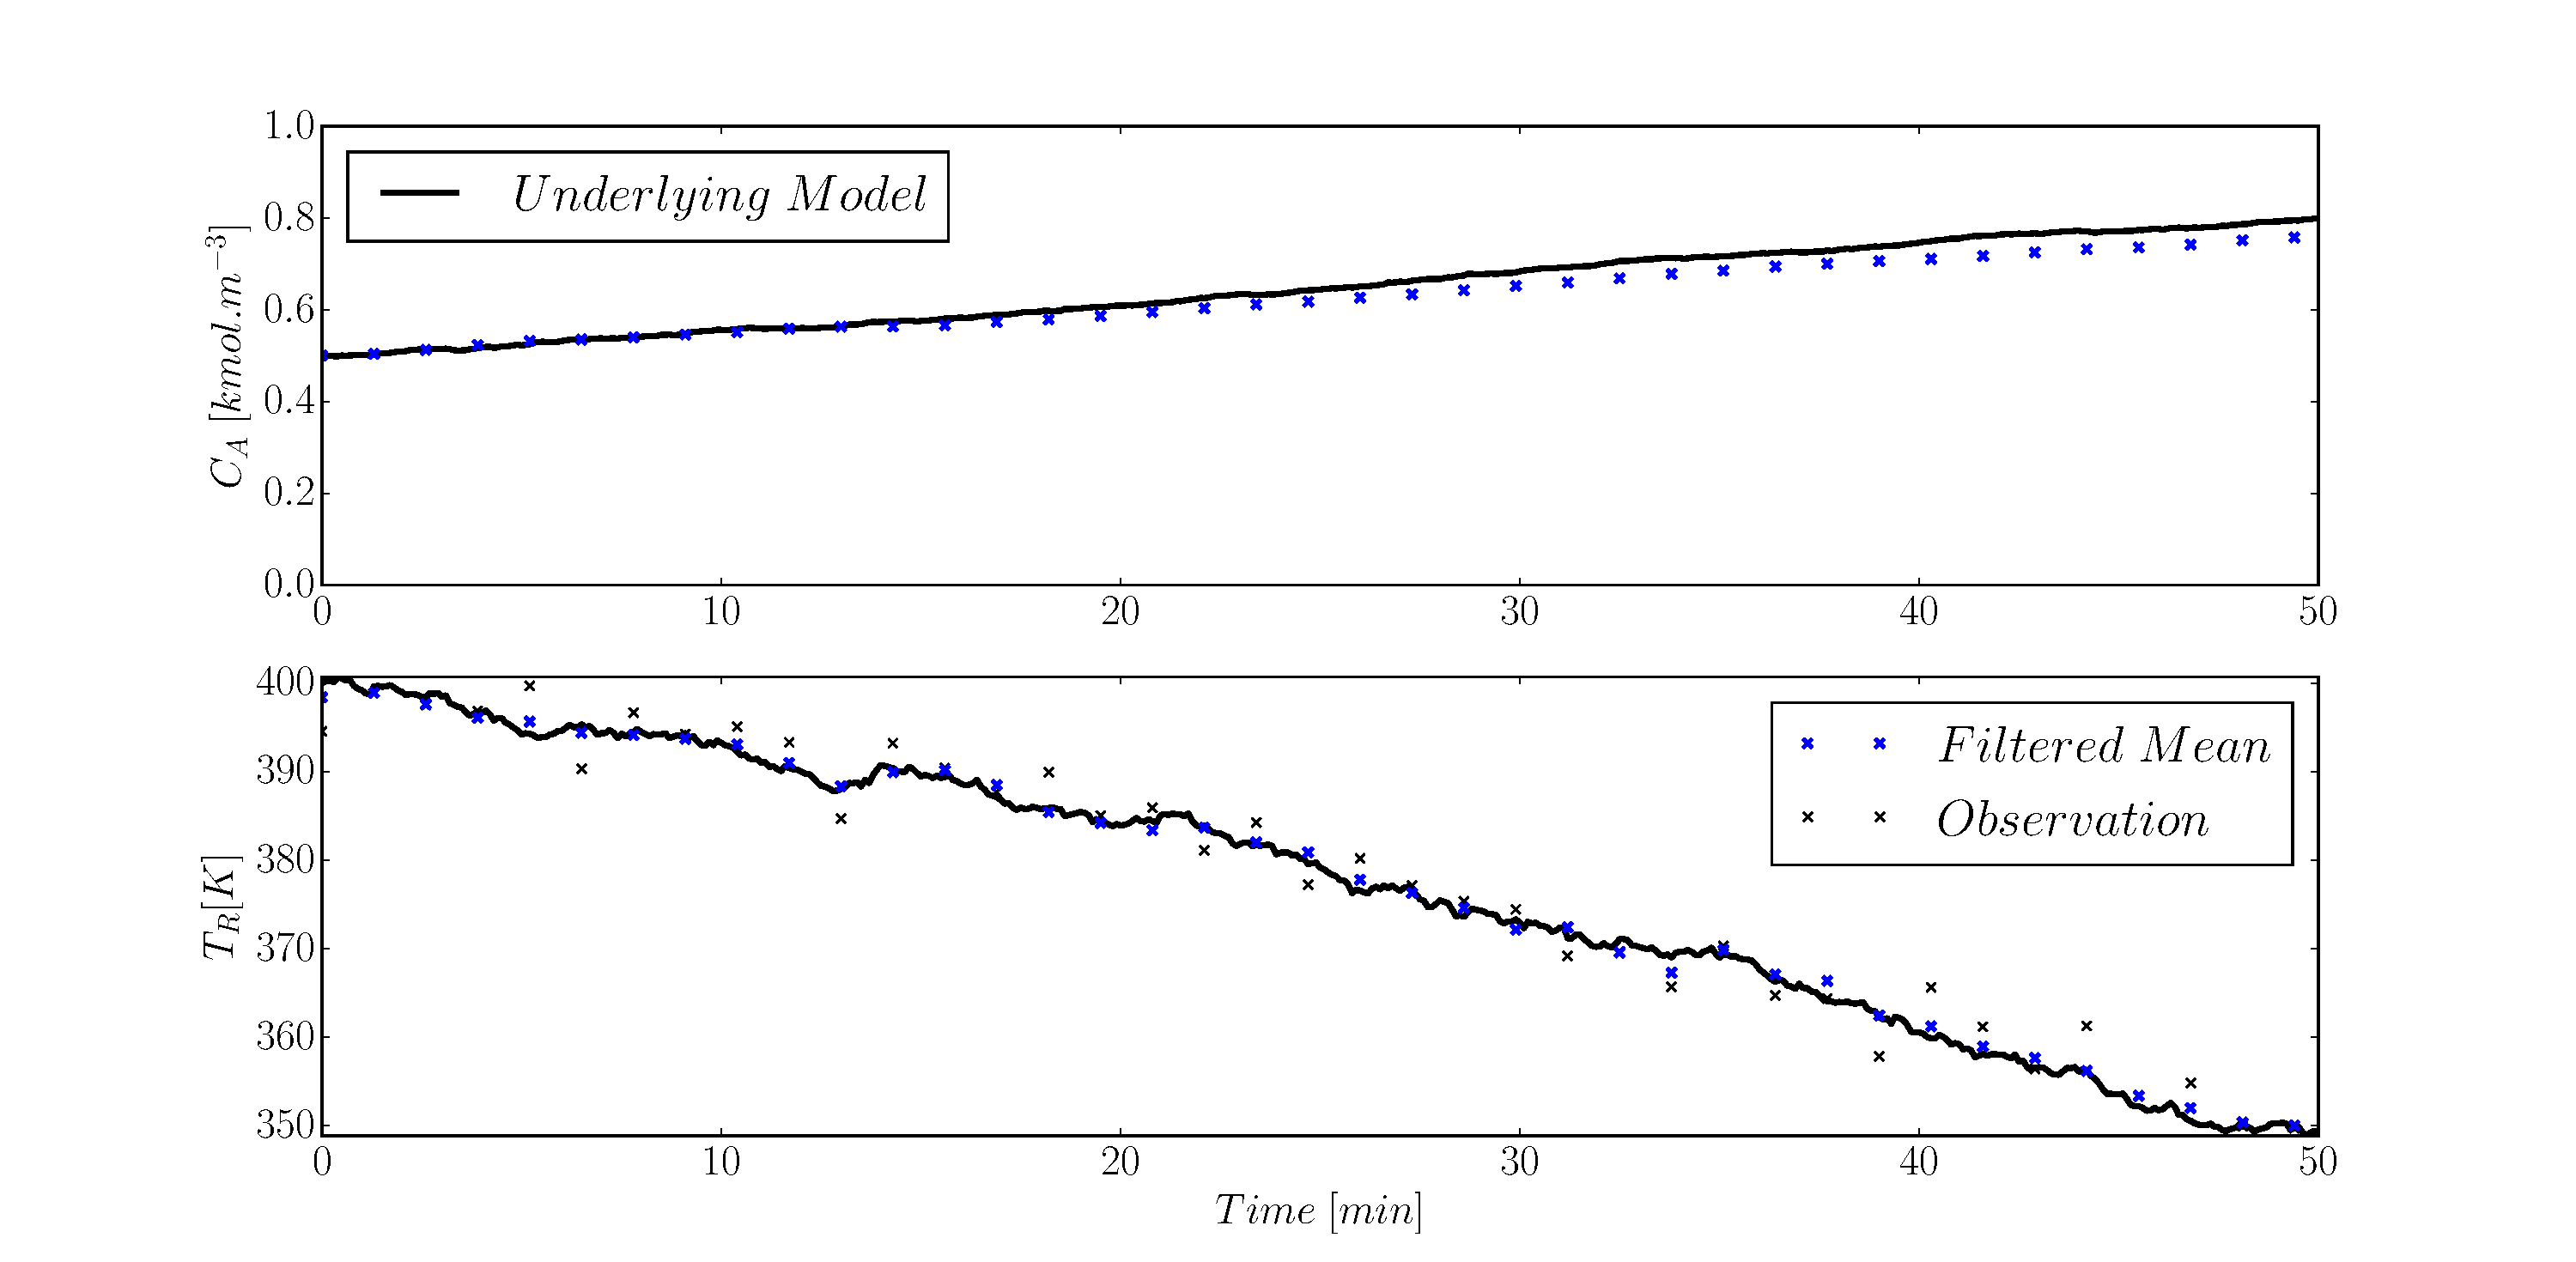
\includegraphics[scale=0.25]{pf_m1_time.pdf}
\caption{Time series state estimates using the Particle Filter on the nonlinear CSTR model with initial condition $(0.5, 400)$ and measuring only temperature. The filter uses 200 particles.}
\label{fig_pf_m1_time}
\end{figure}
The filter tracks both states reasonable well with a little more variance evident in the unmeasured state. The benefit of using the full nonlinear model is evident here - since the model is more accurate than the previously used linear model the filter infers the concentration more accurately. The average concentration and temperature estimation error is 3.15\% and 0.20\% respectively. Compare this to 22.73\% and 0.47\% over the same simulation time using a Kalman Filter measuring only temperature. The increased accuracy is also reflected in the state space evolution curve in Figure \ref{fig_pf_m1_phase}.
\begin{figure}[H] 
\centering
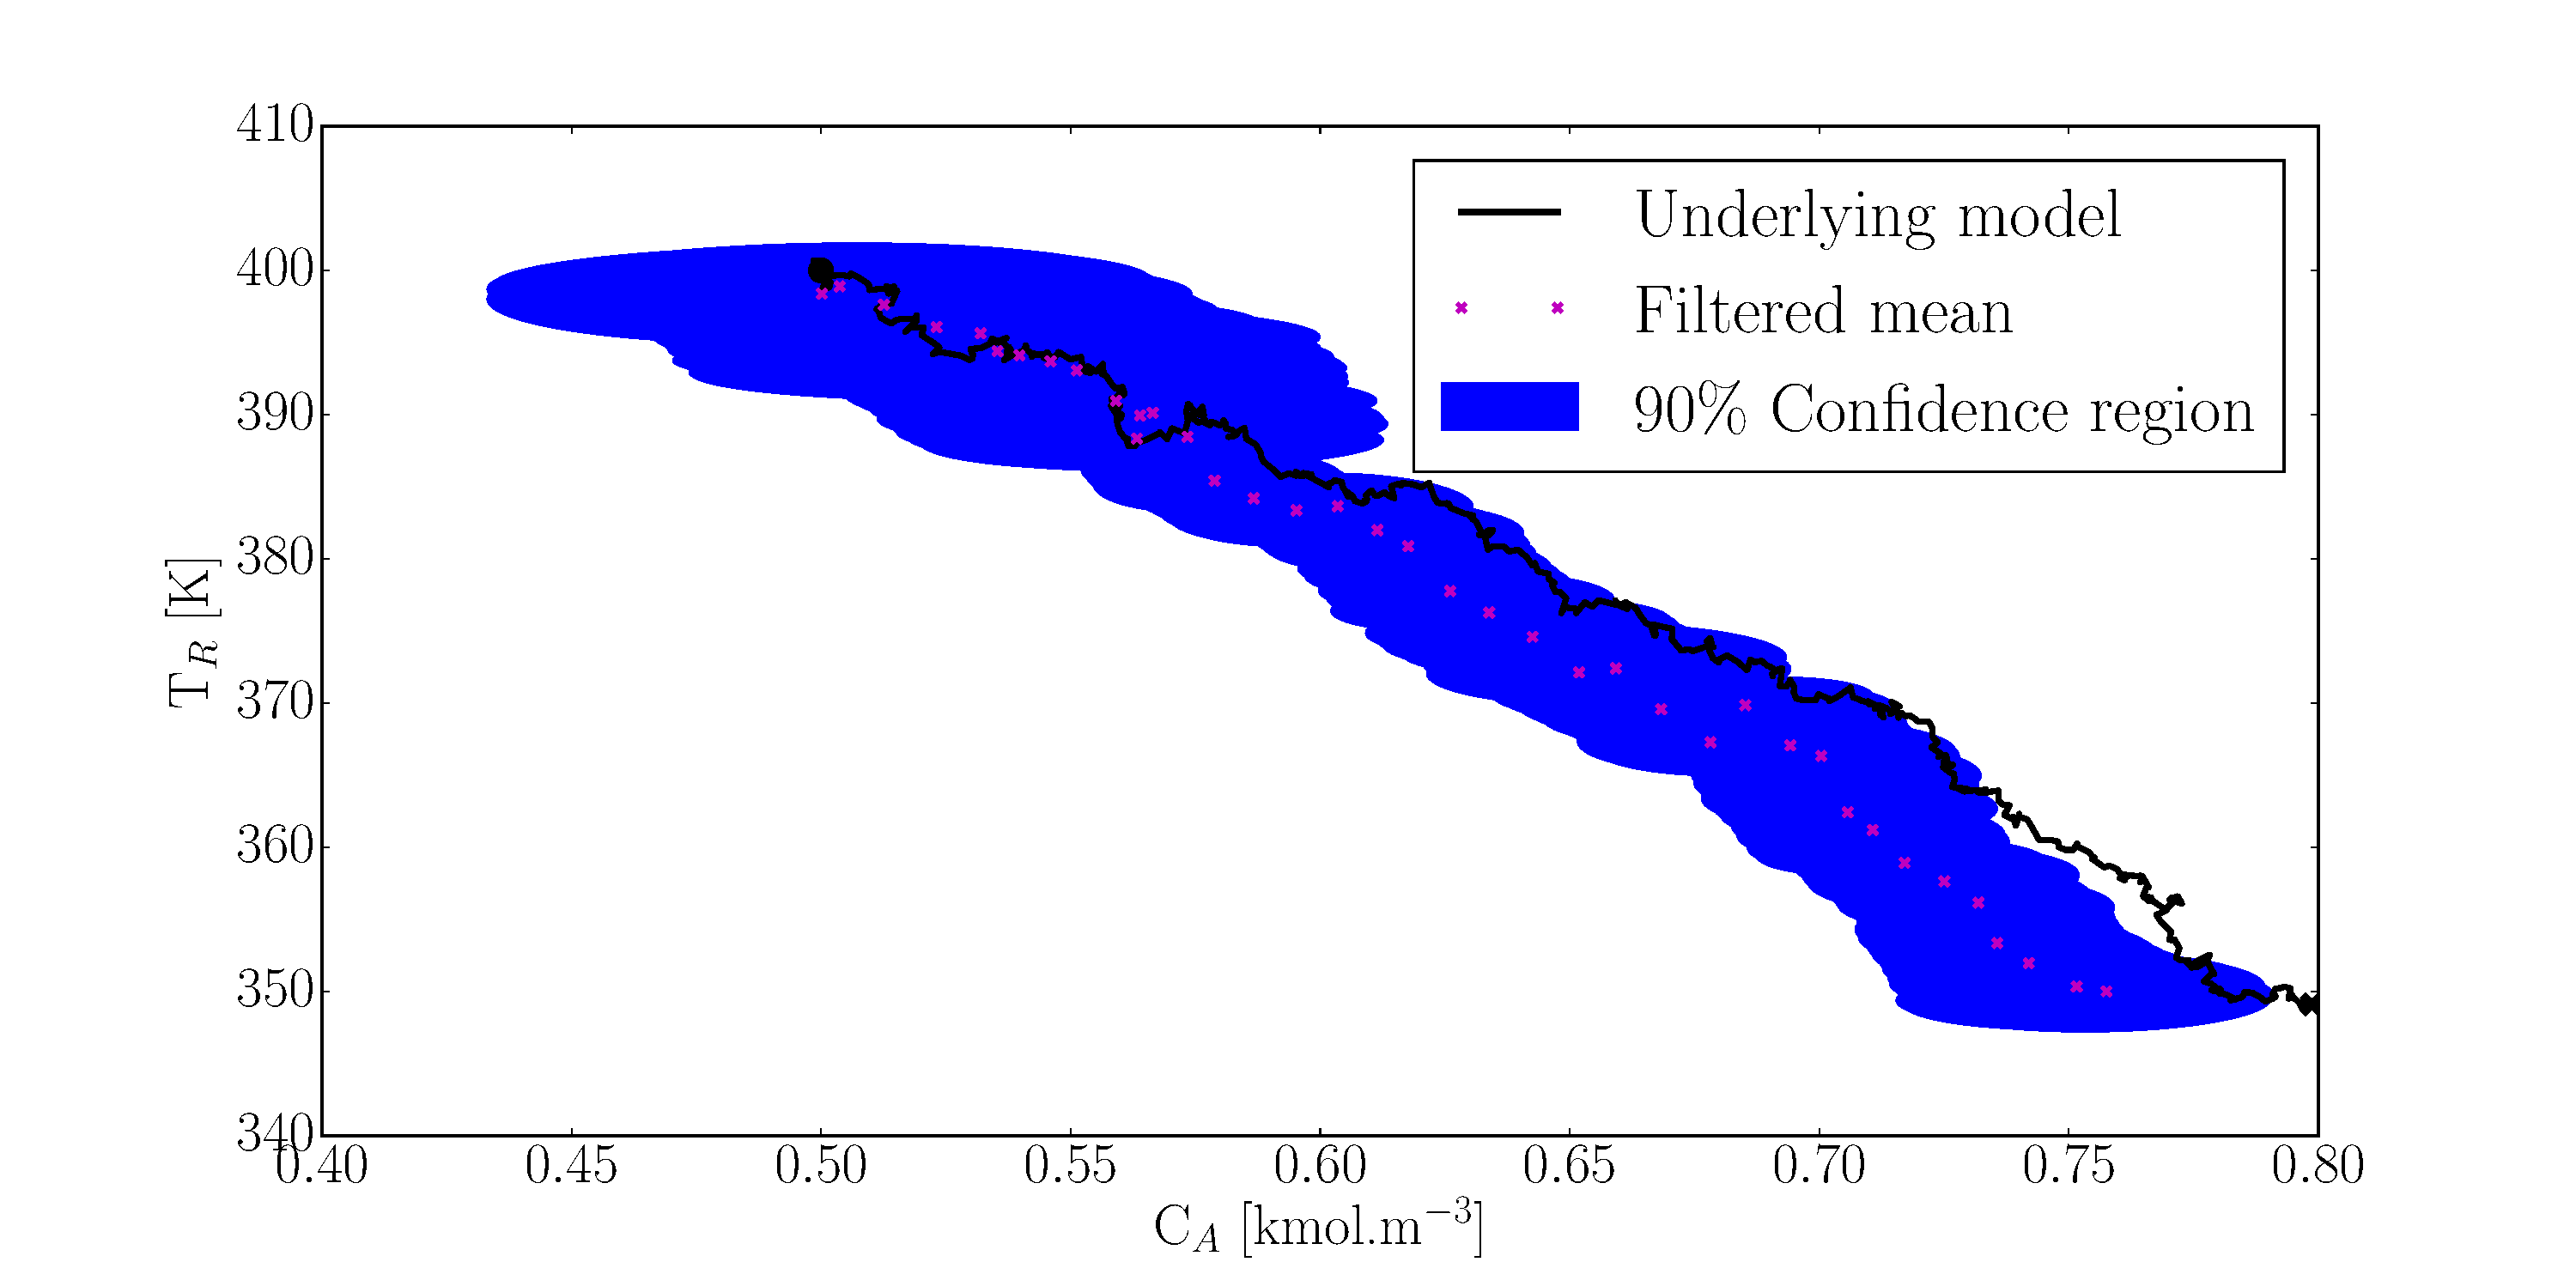
\includegraphics[scale=0.25]{pf_m1_phase.pdf}
\caption{State space evolution of the Particle Filter on the nonlinear CSTR model with initial condition $(0.5, 450)$ and measuring only temperature. The filter uses 200 particles.}
\label{fig_pf_m1_phase}
\end{figure}
We also see in Figure \ref{fig_pf_m1_phase} that the variance of the estimates is quite high (the confidence region is quite big). We expect that by also measuring concentration this will decrease. In Figures \ref{fig_pf_m2_time} and \ref{fig_pf_m2_phase} we incorporate concentration measurement to aid inference. 
\begin{figure}[H] 
\centering
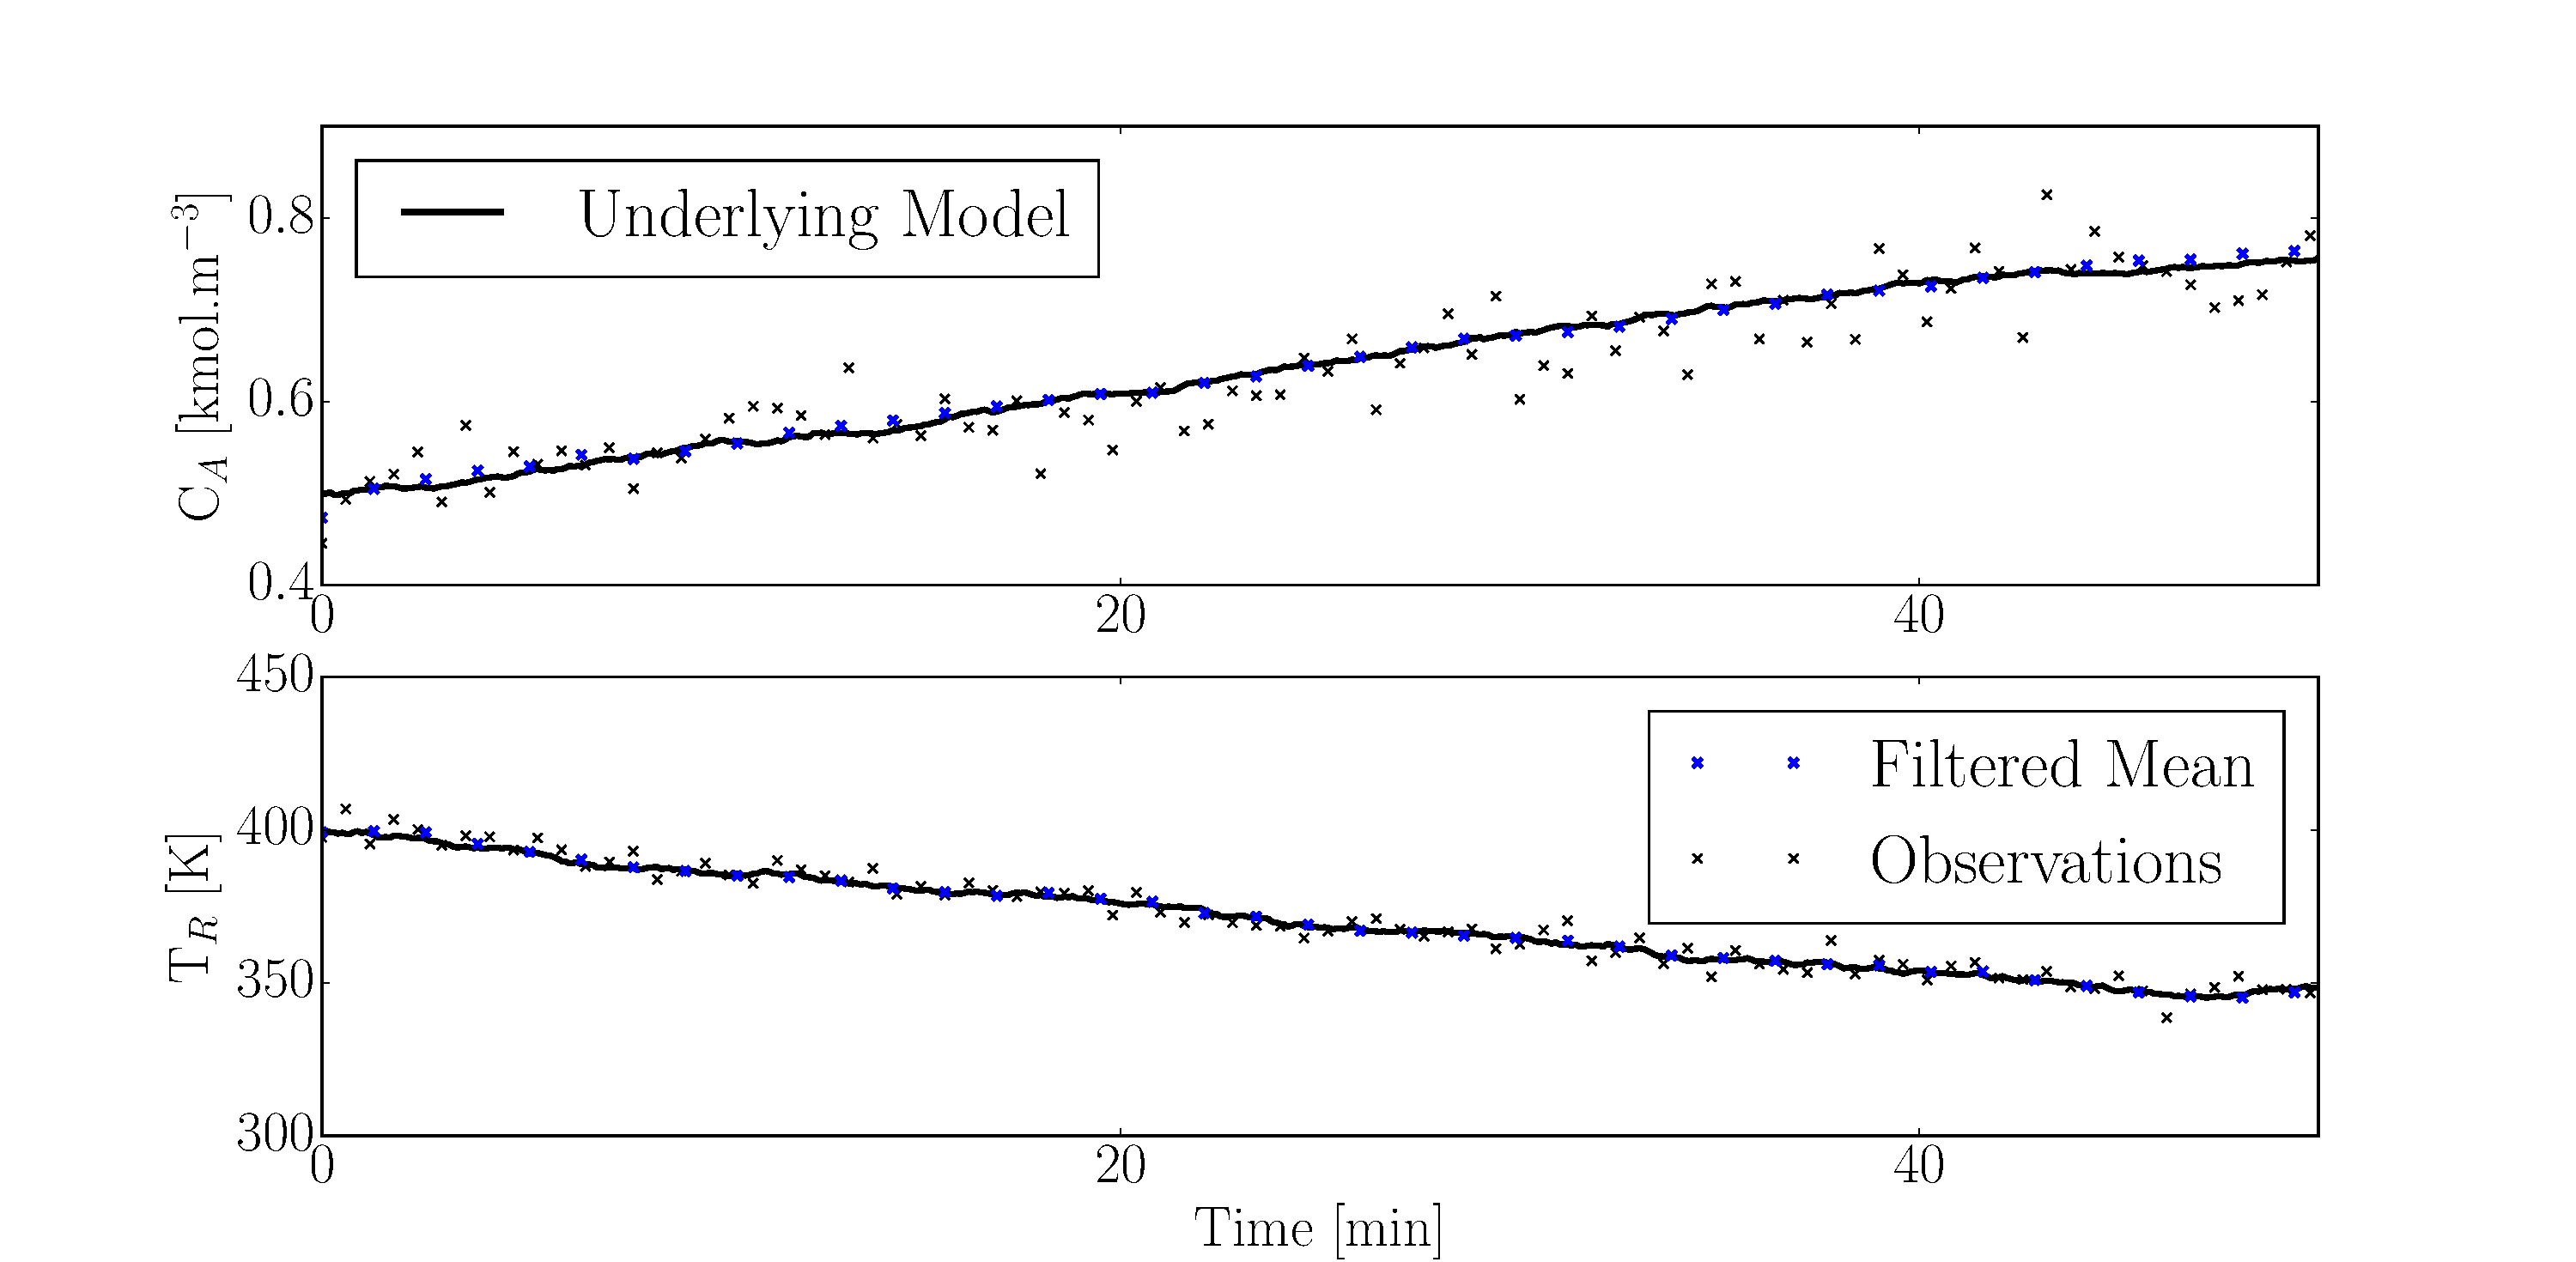
\includegraphics[scale=0.25]{pf_m2_time.pdf}
\caption{Time series state estimates using the Particle Filter on the nonlinear CSTR model with initial condition $(0.5, 450)$ and measuring both states. The filter uses 200 particles.}
\label{fig_pf_m2_time}
\end{figure}
It is clear that that the Particle Filter reliably tracks the state evolution in the presence of plant and measurement noise. The average concentration and temperature estimation error is 0.81\% and 0.21\% respectively. We see that by also measuring the concentration the size of the confidence region decreases in Figure \ref{fig_pf_m2_phase}. 
\begin{figure}[H] 
\centering
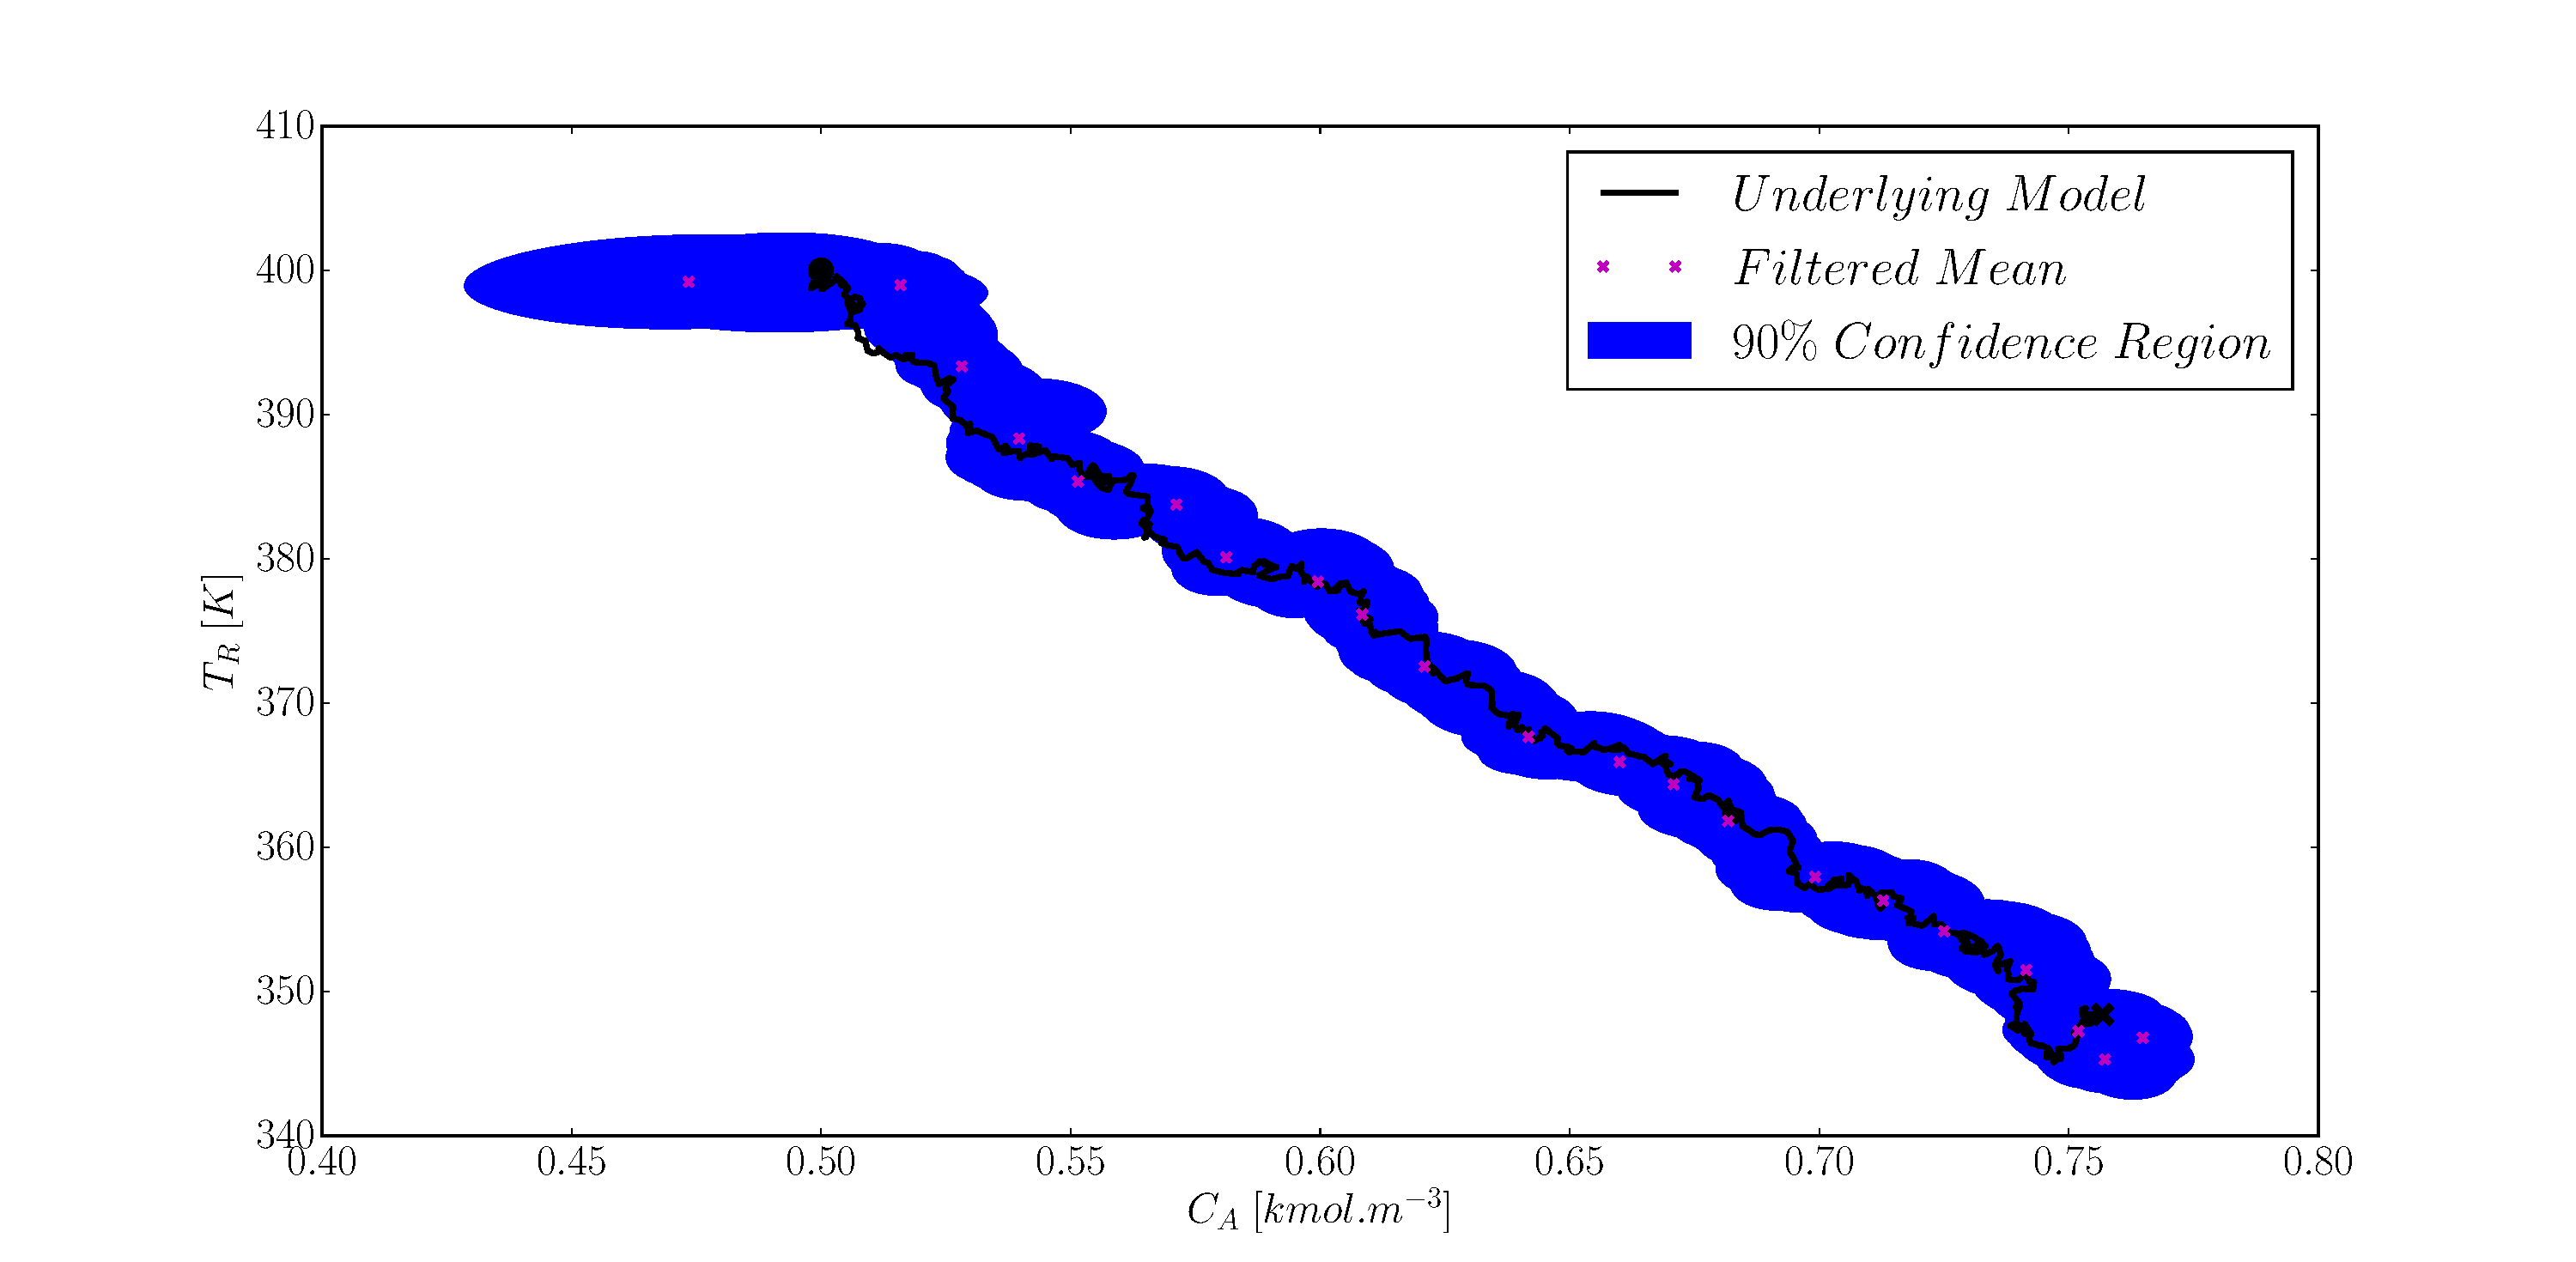
\includegraphics[scale=0.25]{pf_m2_phase.pdf}
\caption{State space evolution of the Particle Filter on the nonlinear CSTR model with initial condition $(0.5, 450)$ and measuring both states. The filter uses 200 particles.}
\label{fig_pf_m2_phase}
\end{figure}
Finally we compare the Particle Filter to the Kalman filter using both temperature and concentration measurements. First we illustrate that if the underlying model is linear and the noise Gaussian the Particle Filter does no better than the Kalman Filter. In Figure \ref{fig_pf_kf_phase1} we see that both the Particle Filter and the Kalman Filter are able to accurately estimate the posterior state distribution over time. Note that we have used 500 particles to meaningfully compare the distribution estimates (the more particles one uses in the Particle Filter the more accurate it becomes).
\begin{figure}[H] 
\centering
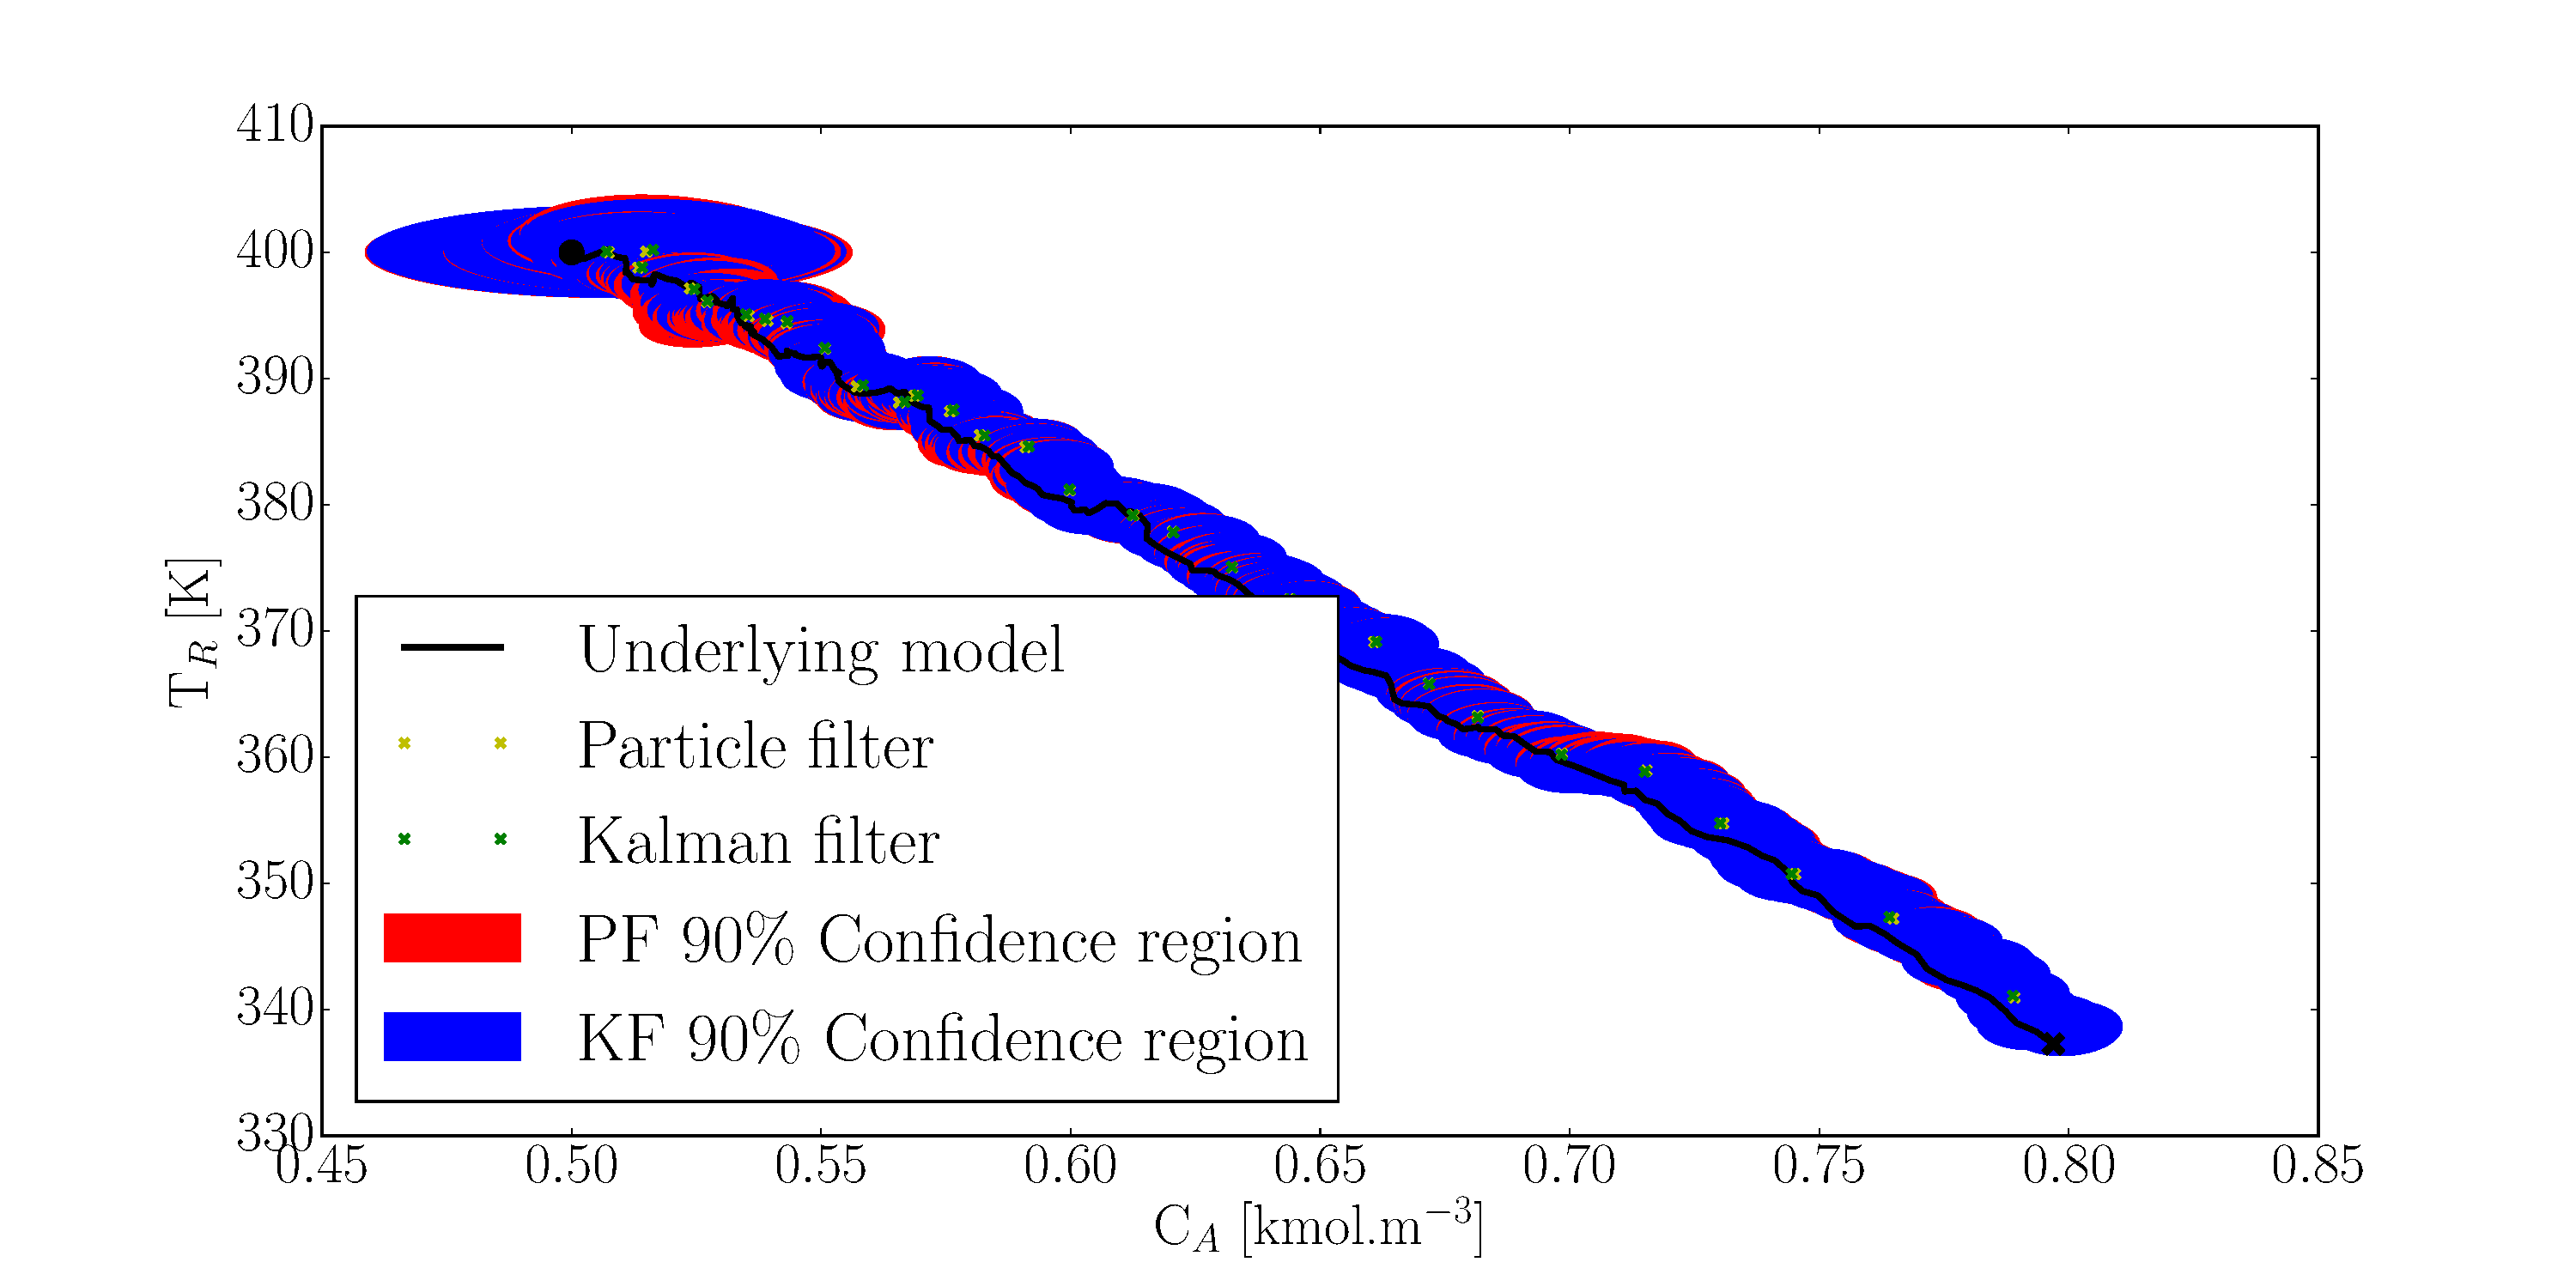
\includegraphics[scale=0.25]{pf_kf_phase1.pdf}
\caption{State space evolution of the Particle Filter and the Kalman Filter on the linear CSTR model with initial condition $(0.5, 400)$ and measuring both temperature and concentration. The Particle Filter uses 500 particles.}
\label{fig_pf_kf_phase1}
\end{figure}
The average concentration and temperature estimation errors for the Particle Filter is 0.93\% and 0.23\% respectively while the corresponding estimation errors for the Kalman Filter is 0.97\% and 0.23\% respectively. Since the confidence region overlaps throughout the entire simulation it is clear that if the underlying model is linear there is no great difference between the two filters from an accuracy point of view. It does however makes sense, from a computational point of view, to use the Kalman Filter: it is well known that the Particle Filter does not perform well in high dimensional problems\cite{snyder}. 

Next we consider the same comparison but change the underlying model to the full non-linear CSTR as shown in Figure \ref{fig_pf_kf_phase2}. The average concentration and temperature estimation errors for the Particle Filter is 0.83\% and 0.19\% respectively while the corresponding estimation errors for the Kalman Filter is 4.50\% and 0.41\% respectively.
\begin{figure}[H] 
\centering
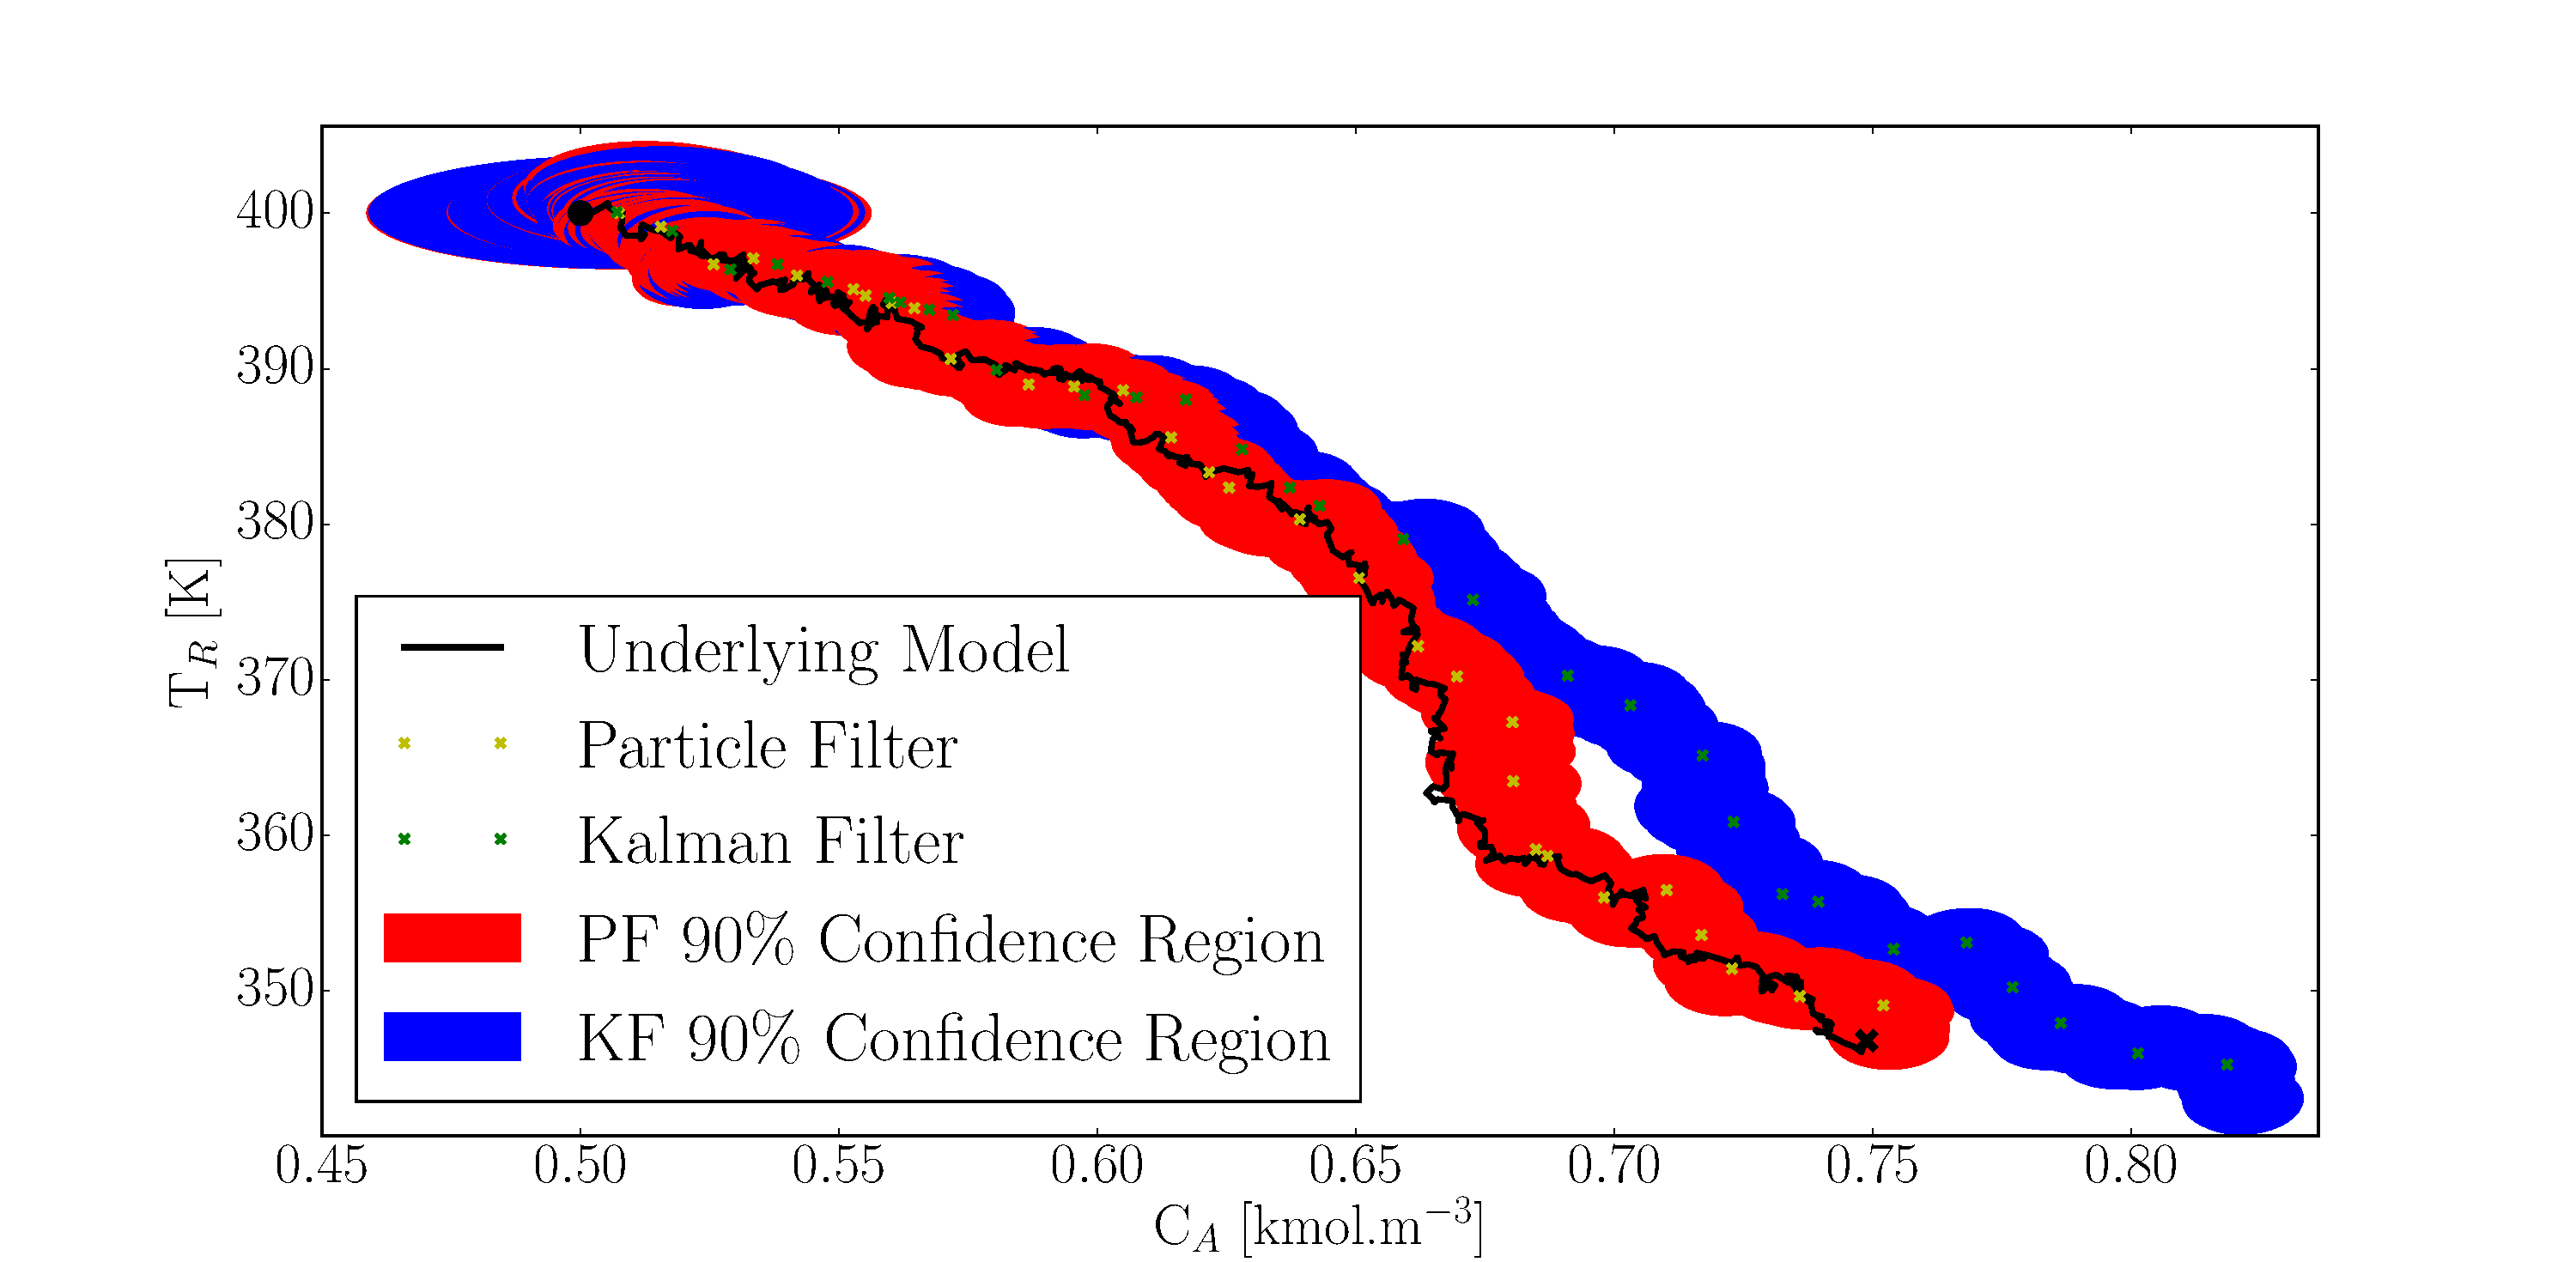
\includegraphics[scale=0.25]{pf_kf_phase2.pdf}
\caption{State space evolution of the Particle Filter and the Kalman Filter on the non-linear CSTR model with initial condition $(0.5, 400)$ and measuring both temperature and concentration. The Particle Filter uses 500 particles.}
\label{fig_pf_kf_phase2}
\end{figure}
Inspecting Figure \ref{fig_pf_kf_phase2} we see that throughout the simulation the Particle Filter's confidence region is smaller. Since we are using a significantly more accurate model for the Particle Filter this is not surprising. Additionally we see that the Kalman Filter state estimates diverge from the true states as the model moves away from the region where the linear model is accurate. The same weakness in the Kalman Filter was discussed in Section \ref{sec_inf_lin_mods} concerning the usage of the linear model.

Therefore, while the Particle Filter may be computationally more expensive to use it is a better filter if the system exhibits non-linearity or non-Gaussian distributions. But, if the system is linear one is better off using the standard Kalman Filter.
\section{Stochastic Linear Control}
\label{sec_linear_control}
In this section we consider the stochastic reference tracking problem. It is required to move the states and manipulated variables of the system, shown in (\ref{eq_lin_system}), to the set point $(x_{sp}, u_{sp})$ by manipulating the input variables $u$.
\begin{equation}
\begin{aligned}
x_{t+1} &= f(x_t, u_t) + w_{t+1}  \\
y_{t+1} &= g(x_{t+1}) + v_{t+1}  
\end{aligned}
\label{eq_lin_system}
\end{equation}
We assume uncorrelated zero mean additive Gaussian noise in both the state function $f$ and the observation function $g$ with known covariances $W$ and $V$ respectively. Clearly it is not possible to achieve perfect control (zero offset at steady state) because of the noise terms, specifically $w_t$. For this reason we need to relax the set point goal a little bit. We will be content if our controller is able to achieve Definition \ref{def_stoch_ref_track_goal}.
\begin{defn}
\textbf{Stochastic Reference Tracking Goal:} Suppose we have designed a controller and set $\delta > 0$ as a controller benchmark. If there exists some positive number $t^* < \infty$ such that $\forall~t > t^*$ the controller input causes $\mathbb{E}[(x_t-x_{sp})^TQ(x_t-x_{sp}) + (u_t-u_{sp})^TR(u_t-u_{sp})] < \delta$ we will have satisfied the Stochastic Reference Tracking Goal given $\delta$.
\label{def_stoch_ref_track_goal}
\end{defn}
While Definition \ref{def_stoch_ref_track_goal} is pleasing from a theoretical point of view, it is not easy to design a controller to specifically satisfy a given $\delta$. We again simplify our goal somewhat: we will be content if the controller we design (without a specific $\delta$ in mind) can satisfy Definition \ref{def_stoch_ref_track_goal} for some suitably small resultant  $\delta$. Intuitively, we would like the mean of the states and inputs to be ``close enough" to the set points. 

In this section we limit ourselves by only considering controllers developed using a single linear model of the underlying, possibly nonlinear, system functions $f$ and $g$. The linearised model control is based upon is shown in (\ref{eq_lin_system_control}) and is subject to the same noise as (\ref{eq_lin_system}).
\begin{equation}
\begin{aligned}
x_{t+1} &= Ax_t + Bu_t + w_{t+1}  \\
y_{t+1} &= Cx_{t+1} + v_{t+1}  
\end{aligned}
\label{eq_lin_system_control}
\end{equation}
We will endeavour to develop predictive controllers using the Graphical Models of Section \ref{sec_inf_lin_mods} and \ref{sec_inf_nonlin_mods}.

\subsection{Unconstrained Stochastic Control}
Our first goal is to solve the problem in (\ref{eq_mpc_unconstrained_linmod}) given the current state estimate $x_0$. If the system is controllable then solving (\ref{eq_mpc_unconstrained_linmod}) will satisfy the linear unconstrained Stochastic Reference Tracking Goal.
\begin{equation}
\begin{aligned}
&\underset{\mathbf{u}}{\text{min }} J_{LQG}(x_0, \mathbf{u}) = \mathbb{E}\left[ \frac{1}{2}\sum_{k=0}^{N-1} \left( x_k^TQx_k + u_k^TRu_k \right) + \frac{1}{2}x_N^TP_fx_N \right] \\
& \text{subject to } x_{t+1}=Ax_t+Bu_t + w_t \\
& \text{and } y_{t}= Cx_t + v_t \text{ (Observed)}\\
\end{aligned}
\label{eq_mpc_unconstrained_linmod}
\end{equation}
Note that the future inputs $\mathbf{u}=(u_0, u_1,...,u_{T-1})$ are denoted in boldface to emphasise that it could be a vector of vectors. Inspecting (\ref{eq_mpc_unconstrained_linmod}) we see that this is none other than the LQG control problem of Section \ref{sec_lqg_lit}. Therefore we know what the optimal solution should look like.

We start out analysis using the results of Section \ref{sec_inf_lin_mods}. We immediately realise that the optimal linear state estimator is the Kalman Filter. We assume that at every sequential time step we have the current state estimate, supplied by the Kalman Filter, and denote this by $x_0$. Since we are using the Kalman Filter the mean and covariance of the state estimate is well defined. 
\begin{figure}[H] 
\centering
\begin{tikzpicture}

  % Define nodes
  \node[obs] (ya) {$y_{0}$};
  \node[latent, above=of ya] (xa) {$x_{0}$};
  \node[latent, right=of xa] (xb) {$x_1$};
  \node[latent, right=of xb]  (xc) {$x_{2}$};
  \node[det, above=of xa] (da) {$u_{0}$};
  \node[det, above=of xb] (db) {$u_{1}$};
  
  % Connect the nodes
  \edge {da} {xb};
  \edge {db} {xc};
  \edge {xa} {ya};
  \edge {xa} {xb};
  \edge {xb} {xc};
  
\end{tikzpicture}
\caption{Graphical Model for state prediction}
\label{fig_gm_mpc}
\end{figure}
Inspecting Figure \ref{fig_gm_mpc} we note that the state prediction equations derived in Subsection \ref{sec_lin_prediction} are applicable. Thus we can predict the state distributions given the future inputs $\mathbf{u}$.

Before we proceed we prove a very intuitive result in Theorem \ref{thrm_optim_eq}. We will use this to link the predictive controller derived using the results of Section \ref{sec_inf_lin_mods} to the LQR controller derived in Section \ref{sec_lqr_lit}. We provide two proofs, the second of which is more general than the first.
\begin{thrm}
\textbf{Optimisation Equivalence} Suppose we have two real valued convex objective functions $f(x_0,\mathbf{u})$ and $g(x_0, \mathbf{u})$ and we are required to minimise them with respect to $\mathbf{u}$ over the same space where they are both defined: $\mathbf{u}\in \mathcal{U}$ and $x_0 \in \mathcal{X}$. Furthermore, suppose there exists a real number $k \geq 0$ such that $\forall \mathbf{u} \in \mathcal{U}$ we have that $g(x_0, \mathbf{u}) + k = f(x_0, \mathbf{u})$. Finally, assume the existence and uniqueness of the global minimiser for each problem. Then the global minimiser $\mathbf{u}^*$ of $g(x_0, \mathbf{u})$ is also the global minimiser of $f(x_0, \mathbf{u})$.
\label{thrm_optim_eq}
\end{thrm}
\begin{proof}
This proof only holds over functions which are at least twice differentiable. By assumption we know that $\mathbf{u}^*$ is the minimiser of $g(x_0, \mathbf{u})$ given $x_0$. By the necessary conditions for optimality \cite{forst} we know that $\nabla g(x_0, \mathbf{u}^*) = 0$ and that $\nabla ^2 g(x_0, \mathbf{u}^*)$ is positive semi-definite. Since $f$ and $g$ are both twice differentiable and  $g(x_0, \mathbf{u}^*) + k = f(x_0, \mathbf{u}^*)$ it must hold that $\nabla g(x_0, \mathbf{u}^*) = \nabla f(x_0, \mathbf{u}^*)$ and  $\nabla ^2 g(x_0, \mathbf{u}^*) = \nabla ^2 f(x_0, \mathbf{u}^*)$. Since $\nabla ^2 g(x_0, \mathbf{u}^*)$ is positive semi-definite it must be that $\nabla ^2 f(x_0, \mathbf{u}^*)$ is also positive semi-definite. Therefore $\mathbf{u}^*$ is necessarily a minimum of $f$. Since $f$ is convex the minimum must also be a global minimum.
\end{proof}
\begin{proof}
This proof hold over differentiable and non-differentiable objective functions. Suppose not i.e. there exists  $\mathbf{u}_g \in \mathcal{U}$ such that $g(x_0, \mathbf{u}_g) < g(x_0, \mathbf{u})$ $\forall \mathbf{u} \in \mathcal{U}$ but $f(x_0, \mathbf{u}_g) \nless f(x_0, \mathbf{u})$ $\forall \mathbf{u} \in \mathcal{U}$. This implies that for $\mathbf{u}_f \in \mathcal{U}$ the global minimiser of $f$  we have $f(x_0, \mathbf{u}_f) \leq f(x_0, \mathbf{u}_g)$. 

Consider the case where $f(x_0, \mathbf{u}_f) = f(x_0, \mathbf{u}_g)$. This implies that both $\mathbf{u}_f$ and $\mathbf{u}_g$ are global minimisers of $f$ and contradicts our assumption that the global minimiser is unique.

Consider the case where $f(x_0, \mathbf{u}_f) < f(x_0, \mathbf{u}_g)$. Since $g(x_0, \mathbf{u}) + k = f(x_0, \mathbf{u})$ $\forall \mathbf{u} \in \mathcal{U}$ this implies that $g(x_0, \mathbf{u}_f) < g(x_0, \mathbf{u}_g)$. But this contradicts our assumption that $\mathbf{u}_g$ is the global minimiser of $g$.

It must then hold that $f(x_0, \mathbf{u}_g) < f(x_0, \mathbf{u})$ $\forall \mathbf{u} \in \mathcal{U}$. Therefore the global minimiser $\mathbf{u}_g$ of $g(x_0, \mathbf{u})$ also minimises $f(x_0, \mathbf{u})$. Since $f$ is convex the minimum must also be a global minimum.
\end{proof}
Now we are in a position to show the equivalence between the LQR control problem and the LQG control problem using the results of Section \ref{sec_inf_lin_mods}. Theorem \ref{thrm_lqr_lqg_diff} shows how this is possible. It is quite reassuring to note that by starting within the framework of Graphical Models we arrive at the most important contribution of \cite{yan1} and \cite{yan2} in an intuitively simple manner.
\begin{thrm}
\textbf{LQR and LQG Objective Function Difference} Consider the LQR and LQG Objective Functions in (\ref{eq_lqr_obj_func}) and (\ref{eq_lqg_obj_func}) respectively. 
\begin{align}
&J_{LQR}(x_0, \mathbf{u}) = \frac{1}{2}\sum_{k=0}^{N-1} \left( x_k^TQx_k + u_k^TRu_k \right) + \frac{1}{2}x_N^TP_fx_N \label{eq_lqr_obj_func} \\
& \text{with } x_{t+1} = Ax_t +Bu_t \text{ (Observed)} \nonumber\\
& J_{LQG}(x_0, \mathbf{u}) =  \mathbb{E}\left[ \frac{1}{2}\sum_{k=0}^{N-1} \left( x_k^TQx_k + u_k^TRu_k \right) + \frac{1}{2}x_N^TP_fx_N \right] \label{eq_lqg_obj_func} \\
& \text{with } x_{t+1} = Ax_t +Bu_t + w_{t+1} \nonumber \\
& \text{and } y_{t} = Cx_t + v_t \text{ (Observed)} \nonumber
\end{align}
Suppose $x_0$ is the state estimate supplied by the Kalman Filter given the latest observation in the stochastic case. In the deterministic case we have that $x_0 = \mathbb{E}[x_0] = \mu_0$ because we exactly observe the state. Given any input sequence $\mathbf{u} \in \mathcal{U}$, where $\mathcal{U}$ is the shared admissible input space, we have that $J_{LQR}(x_0, \mathbf{u}) + \frac{1}{2}\sum_{k=0}^N \text{tr}(Q\Sigma_k) = J_{LQG}(x_0, \mathbf{u})$ where $ \Sigma_{t+1} = W+A\Sigma_t A^T$ and $\Sigma_0$ is the covariance matrix of the current state given by the Kalman Filter.
\label{thrm_lqr_lqg_diff}
\end{thrm}
\begin{proof}
Expanding the LQG objective function and noting that $\mathbf{u}$ is deterministic we have (\ref{eq_expanded_obj}). Note that the conditional expectations in the expansion originate from the graphical model in Figure \ref{fig_gm_mpc} due to the first order Markov assumption. 
\begin{equation}
\begin{aligned}
J_{LQG}(x_0, \mathbf{u}) &= \frac{1}{2} \mathbb{E}\left[x_0^TQx_0 + u_0^TRu_0 \right] + \frac{1}{2} \mathbb{E}\left[x_1^TQx_1 + u_1^TRu_1 |x_0\right] + ... \\ &+ \frac{1}{2} \mathbb{E}\left[x_{N-1}^TQx_{N-1} + u_{N-1}^TRu_{N-1}|x_{N-2} \right] + \frac{1}{2} \mathbb{E}\left[x_N^TP_fx_N|x_{N-1} \right] \\
&= \frac{1}{2} \mathbb{E}\left[x_0^TQx_0\right] +\frac{1}{2} u_0^TRu_0 + \frac{1}{2} \mathbb{E}\left[x_1^TQx_1|x_0\right] + \frac{1}{2}u_1^TRu_1 + ... \\ &+ \frac{1}{2} \mathbb{E}\left[x_{N-1}^TQx_{N-1}|x_{N-2} \right]+ \frac{1}{2}u_{N-1}^TRu_{N-1} + \frac{1}{2} \mathbb{E}\left[x_N^TP_fx_N |x_{N-1}\right]
\end{aligned}
\label{eq_expanded_obj}
\end{equation}
We know that $x_0\sim \mathcal{N}(\mu_0, \Sigma_0)$ because the current state estimate comes from the Kalman Filter. This means that we can evaluate the first expected value in (\ref{eq_expanded_obj}) using Theorem \ref{thrm_gaussian_identities} as shown in (\ref{eq_exp1}).
\begin{equation}
\mathbb{E}\left[x_0^TQx_0\right] = \text{tr}(Q\Sigma_0) + \mu_0^TQ\mu_0
\label{eq_exp1}
\end{equation} 
Now we turn out attention to the second expected value in (\ref{eq_expanded_obj}). First note that because we have $x_0$ and $\mathbf{u}$ we can use the result from Section \ref{sec_lin_prediction} to predict (optimally) the distribution of $x_1$. Therefore we know that $x_1 \sim \mathcal{N}(A\mu_0+Bu_0, W+A\Sigma_0 A^T)$. Now we let $\mu_1 = A\mu_0+Bu_0$ and $\Sigma_0 = W+A\Sigma_0 A^T$. Then by using Theorem \ref{thrm_gaussian_identities} as before we have (\ref{eq_exp2}).
\begin{equation}
\mathbb{E}\left[x_1^TQx_1|x_0\right] = \text{tr}(Q\Sigma_1) + \mu_1^TQ\mu_1
\label{eq_exp2}
\end{equation} 
Note that $\text{tr}(Q\Sigma_1)$ does not depend on $u_0$ but only on the initial state estimate $x_0$ which is independent of the future inputs $\mathbf{u}$. Notice that we can continue in this manner to simplify the LQG objective function to (\ref{eq_simpl_obj_func}).
\begin{equation}
\begin{aligned}
&J_{LQG}(x_0, \mathbf{u}) = \frac{1}{2}\sum_{k=0}^{N-1} \left( \mu_k^TQ\mu_k + u_k^TRu_k \right) + \frac{1}{2}\mu_N^TP_f\mu_N + \frac{1}{2}\sum_{k=0}^N \text{tr}(Q\Sigma_k) \\
&\text{with } \mu_{t+1} = A\mu_t +Bu_t \\
&\text{and } \Sigma_{t+1} = W+A\Sigma_t A^T 
\end{aligned}
\label{eq_simpl_obj_func}
\end{equation}
Now note that except for the last term $J_{LQG}(x_0, \mathbf{u})$ is exactly the same as $J_{LQR}(x_0, \mathbf{u})$. The conclusion follows because $\frac{1}{2}\sum_{k=0}^N \text{tr}(Q\Sigma_k)$ is independent of $\mathbf{u}$. 
\end{proof}
Finally we combine Theorem \ref{thrm_optim_eq} and \ref{thrm_lqr_lqg_diff} to produce Theorem \ref{thrm_lqg_sol} which is the main result of this subsection.
\begin{thrm}
\textbf{Solution of the Finite Horizon LQG control problem} We wish to solve the LQG control problem within the framework of Graphical Models. The full problem is shown in (\ref{eq_lqg_problem_full}).
\begin{equation}
\begin{aligned}
&\underset{\mathbf{u}}{\text{min }} V(x_0, \mathbf{u}) = \mathbb{E}\left[ \frac{1}{2}\sum_{k=0}^{N-1} \left( x_k^TQx_k + u_k^TRu_k \right) + \frac{1}{2}x_N^TP_fx_N \right] \\
& \text{subject to } x_{t+1}=Ax_t+Bu_t + w_t \\
& \text{and } y_{t}= Cx_t + v_t \text{ (Observed)}\\
\end{aligned}
\label{eq_lqg_problem_full}
\end{equation}
The solution of (\ref{eq_lqg_problem_full}) is equivalent to solving the LQR problem with initial state equal to the mean of the initial state estimate from the Kalman Filter.
\label{thrm_lqg_sol}
\end{thrm}
\begin{proof}
We assume that we have the Kalman Filter state estimate for $x_0$. We use Theorem \ref{thrm_lqr_lqg_diff} to prove that given $x_0$ and $\forall \mathbf{u} \in \mathcal{U}$ we have that $J_{LQR}(x_0, \mathbf{u}) + \frac{1}{2}\sum_{k=0}^N \text{tr}(Q\Sigma_k) = J_{LQG}(x_0, \mathbf{u})$ with $\frac{1}{2}\sum_{k=0}^N \text{tr}(Q\Sigma_k) \in \mathbb{R}$ a constant depending only on $x_0$. Thus we can use Theorem \ref{thrm_optim_eq} to prove that we only need to solve for the optimal controller input $\mathbf{u}^0$ using the LQR objective function. Thus we can use Theorem \ref{thrm_lqr_sol} to find $\mathbf{u}$. 
\end{proof}

As we have mentioned before, the Separation Theorem implies that the solution of the LQG control problem is achieved by using the Kalman Filter to optimally estimate the current state and then using that state estimate in the optimal LQR controller. It is reassuring that Theorem \ref{thrm_lqg_sol} is confirmed by this result. The primary benefit of the Graphical Model approach is clear: we have solved the LQG problem without resorting to Stochastic Dynamical Programming.

Under some circumstances it is also possible to extend the result of Theorem \ref{thrm_lqg_sol} to the infinite horizon case as shown in Theorem \ref{thrm_lqg_sol_inf}.
\begin{thrm}
\textbf{Solution of the Infinite Horizon LQG control problem} If the linear model of (\ref{eq_lin_system_control}) is stable then, using, with some minor adjustments, Theorems \ref{thrm_optim_eq} and \ref{thrm_lqr_lqg_diff} it is possible to show that the infinite horizon LQG problem is solved in a similar manner: the Kalman Filter state estimate is used in conjunction with the infinite horizon LQR solution. This result can also be obtained by using the Separation Theorem. \label{thrm_lqg_sol_inf}
\end{thrm}
To clarify why it is important that the linear system, i.e. the matrix $A$, is stable, consider the quantity $\frac{1}{2}\sum_{k=0}^N \text{tr}(Q\Sigma_k)$. If it is unbounded the optimisation minimum will tend to infinity. Inspecting $\Sigma_{t+1} = W+A\Sigma_t A^T$ we see that $||\Sigma_{\infty}||$ will be unbounded if $||A\Sigma_t A^T||$ becomes unbounded ($W$ is a constant). Note that $||\cdot||$ is some matrix norm. It can be shown that if the eigenvalues of $A$ are less than unity i.e. the linear model is stable, then $||A\Sigma_{t+1}A^T|| \leq ||A\Sigma_{t+1}A^T||$ which implies that $\frac{1}{2}\sum_{k=0}^N \text{tr}(Q\Sigma_k)$ is bounded and the optimisation is reasonable.


\subsection{Constrained Stochastic Control}
The goal of this section is to solve the stochastic constrained optimisation problem shown in (\ref{eq_mpc_constrained_linmod}). We assume that the underlying system is linear and the probability distributions are Gaussian\footnote{From the results of Section \ref{sec_inf_lin_mods} the probability distributions will be Gaussian if the system dynamics are linear. However, it is well known \cite{mac} that MPC is not in general a linear controller. From an analytical point of view this is problematic. We assume that the nonlinearity introduced by the MPC is negligible.}. We also restrict our analysis to affine constraints. Note that we only include one constraint in the succeeding analysis however, additional constraints are handled in exactly the same way as we will show.
\begin{equation}
\begin{aligned}
&\underset{\mathbf{u}}{\text{min }} \mathbb{E}\left[ \frac{1}{2}\sum_{k=0}^{N-1} \left( x_k^TQx_k + u_k^TRu_k \right) + \frac{1}{2}x_N^TP_fx_N \right] \\
& \text{subject to } x_{t+1}=Ax_t+Bu_t + w_t \\
& \text{and } y_{t}= Cx_t + v_t \text{ (Observed)}\\
& \text{and } \mathbb{E}[d^Tx_t + e] \geq 0 ~\forall ~t=1,...,N \\
& \text{and } \text{Pr}(d^Tx_t + e \geq 0) \geq p ~\forall ~t=1,...,N\\
\end{aligned}
\label{eq_mpc_constrained_linmod}
\end{equation}
It might seem that the last constraint is a duplicate of the preceding one. Closer inspection reveals their different character. The first inequality constraint requires that the predicted states satisfy the constraint ``on average" while the second inequality constraint requires that the predicted states jointly satisfy the constraint with at least some probability $p$.

Theorem \ref{thrm_affine_expected_const} succinctly shows that it is simple to convert the first stochastic constraint in (\ref{eq_mpc_constrained_linmod}) to a linear deterministic constraint.
\begin{thrm}
\textbf{Affine Expected Value Constraints} Suppose we have a stochastic variable $x$ with a known Gaussian distribution. Then the stochastic constraint $\mathbb{E}[d^Tx + e] \geq 0$ simplifies to the deterministic constraint $d^T\mu + e \geq 0$ where $\mathbb{E}[x]= \mu$ is the mean of the stochastic variable.
\label{thrm_affine_expected_const}
\end{thrm}
\begin{proof}
We know that $x$ is a Gaussian stochastic variable. By the results of Section \ref{thrm_gaussian_identities} we know that $\mathbb{E}[d^Tx + e] =d^T\mu + e$. This immediately implies the Theorem.
\end{proof}
It is interesting to pause here for a moment and consider Theorem \ref{thrm_lqg_sol} and Theorem \ref{thrm_affine_expected_const} applied to a problem of the form (\ref{eq_mpc_constrained_linmod_noprob}). We assume that the current state estimate is available at each time step and that $\mathbb{E}[x_0]=\mu_0$.
\begin{equation}
\begin{aligned}
&\underset{\mathbf{u}}{\text{min }} \mathbb{E}\left[ \frac{1}{2}\sum_{k=0}^{N-1} \left( x_k^TQx_k + u_k^TRu_k \right) + \frac{1}{2}x_N^TP_fx_N \right] \\
& \text{subject to } x_{t+1}=Ax_t+Bu_t + w_t \\
& \text{and } y_{t}= Cx_t + v_t \text{ (Observed)}\\
& \text{and } \mathbb{E}[d^Tx_t + e] \geq 0 ~\forall ~t=1,...,N \\
\end{aligned}
\label{eq_mpc_constrained_linmod_noprob}
\end{equation}
It is clear that by applying those two theorems it is possible to rewrite (\ref{eq_mpc_constrained_linmod_noprob}) as (\ref{eq_mpc_constrained_linmod_deter_noprob}).
\begin{equation}
\begin{aligned}
&\underset{\mathbf{u}}{\text{min }} \frac{1}{2}\sum_{k=0}^{N-1} \left( \mu_k^TQ\mu_k + u_k^TRu_k \right) + \frac{1}{2}\mu_N^TP_f\mu_N + \frac{1}{2}\sum_{k=0}^N \text{tr}(Q\Sigma_k) \\
& \text{subject to } \mu_{t+1}=A\mu_t + Bu_t \\
& \text{and } d^T\mu_t + e \geq 0 ~\forall ~t=1,...,N\\
\end{aligned}
\label{eq_mpc_constrained_linmod_deter_noprob}
\end{equation}
This implies that the standard deterministic MPC problem (\ref{eq_mpc_constrained_linmod_deter_noprob}) is equivalent to the stochastic MPC problem with affine expected value constraints (\ref{eq_mpc_constrained_linmod_noprob}) under the assumptions of linearity and normality. This suggests that if probability constraints are not required that standard deterministic MPC will be sufficient for control.

Theorem \ref{thrm_mahala_dist} is a necessary step before we can convert the last stochastic inequality constraint of (\ref{eq_mpc_constrained_linmod}) into a nonlinear deterministic constraint.
\begin{thrm}
\textbf{Shortest Squared Mahalanobis Distance between a Hyperplane and a Point} Suppose we are given a symmetric positive semi-definite matrix $S$ and a point $y$. The shortest squared Mahalanobis Distance between $y$ and the hyperplane $b^Tx+c=0$ is given by $\frac{(b^Ty+c)^2}{b^TSb}$.
\label{thrm_mahala_dist}
\end{thrm}
\begin{proof}
It is natural to formulate Theorem \ref{thrm_mahala_dist} as an optimisation problem as shown in (\ref{eq_mahala_optim}). \begin{equation}
\begin{aligned}
&\underset{x}{\text{min }} (x-y)^TS^{-1}(x-y)\\
& \text{subject to } b^Tx+c = 0\\
\end{aligned}
\label{eq_mahala_optim}
\end{equation}
Note that $S$ and therefore also $S^{-1}$ is symmetric. Using conventional calculus we have $\nabla f(x) = (S^{-1} + {S^{-1}}^T)x - 2S^{-1}y = 2S^{-1}x - 2S^{-1}y$ and $\nabla g(x) = b^T$. Using the method of Lagrangian Multipliers \cite{forst} we have the system of equations (\ref{eq_lagrange_eqs})
\begin{equation}
\begin{aligned}
2S^{-1}x - 2S^{-1}y + \lambda b = 0 \\
b^Tx+c = 0
\end{aligned}
\label{eq_lagrange_eqs}
\end{equation}
This can be rewritten in block matrix form as shown in (\ref{eq_lagrange_block}).
\begin{equation}
\begin{pmatrix}
2S^{-1} & b \\ b^T & 0
\end{pmatrix} \begin{pmatrix}
x \\ \lambda
\end{pmatrix} = \begin{pmatrix}
2S^{-1}y \\ -c
\end{pmatrix}
\label{eq_lagrange_block}
\end{equation}
The special structure of the left hand side matrix in (\ref{eq_lagrange_block}) allows us to analytically compute the inverse (see Theorem \ref{thrm_block_inv} in Section \ref{sec_block}) as shown in (\ref{eq_lagrance_block_inverse}).
\begin{equation}
\begin{pmatrix}
2S^{-1} & b \\ b^T & 0
\end{pmatrix}^{-1} = \begin{pmatrix}
\frac{1}{2}S(I-\frac{bb^TS}{b^TSb}) & \frac{Sb}{b^TSb} \\ \frac{b^TS}{b^TSb} & -\frac{2}{b^TSb}
\end{pmatrix}
\label{eq_lagrance_block_inverse}
\end{equation}
To find the arguments which satisfy (\ref{eq_lagrange_eqs}) we solve (\ref{eq_lagrange_args}) which is equivalent to solving the system of linear equations in (\ref{eq_lagrange_block}).
\begin{equation}
\begin{pmatrix}
\frac{1}{2}S(I-\frac{bb^TS}{b^TSb}) & \frac{Sb}{b^TSb} \\ \frac{b^TS}{b^TSb} & -\frac{2}{b^TSb} \end{pmatrix} \begin{pmatrix}
2S^{-1}y \\ -c
\end{pmatrix} = \begin{pmatrix}
S(I-\frac{bb^TS}{b^TSb})S^{-1}y - c\frac{Sb}{b^TSb} \\
2(\frac{b^TS}{b^TSb} + \frac{c}{b^TSb})
\end{pmatrix}
\label{eq_lagrange_args}
\end{equation}
Therefore, the arguments which minimise (\ref{eq_mahala_optim}) are $x^* = S(I-\frac{bb^TS}{b^TSb})S^{-1}y - c\frac{Sb}{b^TSb}$. Substituting this into the objective function we have (\ref{eq_lagrange_min}).
\begin{equation}
\begin{aligned}
&\left(x^*-y\right)^TS^{-1}\left(x^*-y\right) \\ 
&= \left(S\left(I-\frac{bb^TS}{b^TSb}\right)S^{-1}y - c\frac{Sb}{b^TSb}-y\right)^TS^{-1}\left( S \left(I-\frac{bb^TS}{b^TSb}\right)S^{-1}y - c \frac{Sb}{b^TSb}-y\right) \\ 
&= \left(\frac{Sbb^Ty}{b^TSb} + c\frac{Sb}{b^TSb}\right)^TS^{-1}\left(\frac{Sbb^Ty}{b^TSb}+ c\frac{Sb}{b^TSb}\right) \\
&= \frac{(Sb)^T}{b^TSb}\left( b^Ty+c \right)^TS^{-1}\frac{Sb}{b^TSb}\left(b^Ty+c\right) \\
&= \frac{b^TS}{b^TSb}\left(b^Ty+c\right)^T\frac{b}{b^TSb}\left(b^Ty+c\right) \\
&= \left(b^Ty+c\right)^T\frac{b^TSb}{(b^TSb)^2}\left(b^Ty+c\right) \\
&= \frac{(b^Ty+c)^T(b^Ty+c)}{b^TSb} \\
&= \frac{(b^Ty+c)^2}{b^TSb}
\end{aligned}
\label{eq_lagrange_min}
\end{equation}
We can conclude that the shortest squared Mahalanobis Distance between a point $y$ and the constraint of (\ref{eq_mahala_optim}) is $\frac{(b^Ty+c)^2}{b^TSb}$.
\end{proof}
In Theorem \ref{thrm_chance_cons} we apply Theorem \ref{thrm_mahala_dist} to convert the stochastic constraints into nonlinear deterministic constraints.
\begin{thrm}
\textbf{Gaussian Affine Chance Constraints} If the underlying distribution of a random variable $x$ is Gaussian then the chance constraint $\text{Pr}(d^Tx + e \geq 0) \geq p$ can be rewritten as the deterministic constraint $\frac{(d^T\mu+e)^2}{d^TSd} \geq k^2$ where $k^2$ is the (constant) critical value of the inverse cumulative Chi-Squared Distribution with the degrees of freedom equal to the dimensionality of $x$ such that $\text{Pr}(\mathcal{X} \leq k^2) = p$. 
\label{thrm_chance_cons}
\end{thrm}
\begin{proof}
Intuitively Theorem \ref{thrm_chance_cons} posits that if the shortest squared Mahalanobis distance is further away than some threshold $k^2$ the chance constraint $\text{Pr}(dx + e \geq 0) \geq p$ will be satisfied. Since $x$ is a Gaussian stochastic variable we have that $\mathbb{E}[x] =\mu$ and $\text{var}[x]=\Sigma$. Let $\Omega = \{x \in \mathbb{R}^n~|~(x-\mu)^T\Sigma^{-1}(x-\mu) \leq k^2\}$ and $k^2$ be the critical value such that for the Chi-Squared Distribution with degrees of freedom equal to the dimension of $x$ we have that $\text{Pr}(\mathcal{X} \leq k^2) = p$. Then it is well known \cite{mahala2} that $\int_{\Omega}p(x|\mu, \Sigma)dx = p$ where $p(\cdot|\mu, \Sigma)$ is the multivariate Gaussian probability distribution function of $x$. If the shortest squared Mahalanobis Distance from the mean of $x$ is further away from the affine constraint $d^Tz+e=0$ than $k^2$ it implies that the curve of the function $h(z) = (z-\mu)^T\Sigma^{-1}(z-\mu) = k^2$ does not intersect with the constraint. This implies, with at least a probability of $p$, that the chance constraint will not be violated because the ``confidence ellipse" does not intersect the constraint. See Figure for a diagram of the principle behind Theorem \ref{thrm_chance_cons} \cite{mahala1}. 
\textbf{insert picture}
\end{proof}
It is interesting to note the striking similarity between the work in \cite{vanhessem1} and \cite{vanhessem2} and Theorem \ref{thrm_chance_cons} given that we started analysing the problem within the framework of Graphical Models. The additional benefit of Theorem \ref{thrm_chance_cons} is that it formulates the stochastic constraint as a function of the statistical Mahalanobis Distance measure. This is useful because it lends a statistical interpretation to Theorem \ref{thrm_chance_cons} even if the underlying distribution is non-Gaussian.

In Theorem \ref{thrm_mpc_stoch_to_det} we combine and elaborate on the work of \cite{yan1}, \cite{vanhessem1} to yield a QP MPC which exactly satisfies the stochastic MPC in (\ref{eq_mpc_constrained_linmod}) given the assumptions of linearity and normality. Note that the dimensionality of the problem is arbitrary.
\begin{thrm}
\textbf{Conversion of the Stochastic MPC formulation to the standard deterministic QP MPC formulation} Under the assumptions of linearity and Gaussian distributions we can reformulate the stochastic MPC problem shown in (\ref{eq_mpc_constrained_linmod}) as a standard deterministic QP MPC problem shown in (\ref{eq_mpc_constrained_linmod_deter}).
\begin{equation}
\begin{aligned}
&\underset{\mathbf{u}}{\text{min }} \frac{1}{2}\sum_{k=0}^{N-1} \left( \mu_k^TQ\mu_k + u_k^TRu_k \right) + \frac{1}{2}\mu_N^TP_f\mu_N + \frac{1}{2}\sum_{k=0}^N \text{tr}(Q\Sigma_k) \\
& \text{subject to } \mu_{t+1}=A\mu_t + Bu_t \\
& \text{and } \Sigma_{t+1} = W+A\Sigma_t A^T \\
& \text{and } d^T\mu_t + e \geq k\sqrt{d^T \Sigma_t d} ~\forall ~t=1,...,N\\
\end{aligned}
\label{eq_mpc_constrained_linmod_deter}
\end{equation}
\label{thrm_mpc_stoch_to_det}
Other deterministic constraints, e.g. on the input, can be added as usual. Note that we have assumed that the initial state estimate $x_0$ is available in the form of its mean, $\mu_0$,  and covariance, $\Sigma_0$. It is straightforward to include more chance constraints. Since each chance constraint is reduced to an inequality constraint which measures the Mahalanobis Distance between the predicted distributions, the resultant feasible points will jointly satisfy all chance constraints.  
\end{thrm}
\begin{proof}
Let the admissible set of controller inputs $\mathcal{U}$ be the same for both the stochastic MPC and the deterministic MPC formulations. Furthermore, let the current state estimate $x_0$ be given. Then by Theorem \ref{thrm_lqr_lqg_diff} the objective function and equality constraints follow. By Theorem \ref{thrm_affine_expected_const} the first inequality constraint in (\ref{eq_mpc_constrained_linmod}) can be reformulated to require that $d^T\mu + e \geq 0$. The last inequality constraint in (\ref{eq_mpc_constrained_linmod}) follows from Theorem \ref{thrm_chance_cons} as shown in (\ref{eq_chance_to_lin}).
\begin{equation}
\begin{aligned}
\frac{(d^T\mu+e)^2}{d^TSd} \geq k^2 &\implies (d^T\mu+e)^2 \geq k^2 {d^TSd} \\
&\implies d^T\mu+e \geq k \sqrt{d^TSd}
\end{aligned}
\label{eq_chance_to_lin}
\end{equation}
The first line of (\ref{eq_chance_to_lin}) follows because $S$ is positive semi-definite and $d \neq 0$ (otherwise it would not be a constraint), therefore it can be multiplied over the inequality sign like a positive number. The second line follows because of the first inequality constraint: we know that $d^T\mu+e \geq 0$ and therefore we can square root both sides of the inequality constraint. Thus we have the two inequality constraints $d^T\mu+e \geq 0$ and $d^T\mu+e \geq k \sqrt{d^TSd}$. Since $k > 0$ (otherwise we do not have a meaningful chance constraint) we can condense the two inequality constraints into a single constraint: $d^T\mu+e \geq k \sqrt{d^TSd} > 0$ from which the conclusion follows.  
\end{proof}
The beauty of Theorem \ref{thrm_mpc_stoch_to_det} is that no new theory is necessary to analyse the stability and convergence results of the new MPC. This is highly desirable because it allows one to merely ``add" the last inequality constraint to your existing MPC formulation. Most practical MPCs will have some form of state estimation and thus no new parameters are introduced either. Since the problem is in standard QP form it is straightforward to implement and, even more importantly, it is computationally fast because the problem is trivially convex.

In the work by \cite{yan1} and \cite{yan2} it is found that feasibility problems might arise if one uses the predicted covariance estimates in the controller. If the system is unstable the uncertainty in the estimates can grow with time as discussed in Theorem \ref{thrm_lqg_sol_inf}. This can cause the ellipses used in Theorem \ref{thrm_chance_cons} to become too large to fit inside the feasible region. The approach adopted by \cite{yan1} and \cite{yan2} is to only use the one step ahead predicted covariance ($\Sigma_1$) over the entire prediction horizon. This does not ensure feasibility but restricts the growth associated with infeasibility. The drawback of this approach is that it might cause constraint violation because the controller will be more aggressive.  
\subsection{Reference Tracking}
So far we have only dealt with controllers which would drive the system to the origin. The more general situation we are interested in is arbitrary reference point tracking. Fortunately, Section \ref{sec_lit_ref_track} applies without modification because we managed to cast the Stochastic MPC problem into a deterministic MPC problem. 

\subsection{Linear System}
\label{sec_lin_sys_cont}
In this section we consider the problem of controlling a linear system using the stochastic MPC formulation of Theorem \ref{thrm_mpc_stoch_to_det}. More precisely, we assume the linear model linearised about the unsteady operating point of our CSTR example from Section \ref{sec_cstr} accurately represents the underlying system. For the purposes of illustration we will only use the (somewhat unrealistic) system where both states are measured. However, there is no theoretical reason why we cannot use the system where only temperature is measured. The drawback of using the latter system is that inference, as discussed previously, will be worse. The control goal is to steer the concentration, in the sense of Definition \ref{def_stoch_ref_track_goal}, to the unsteady operating point ($C_A = 0.49$ kmol.m$^{-3}$) about which the system was linearised. See Section \ref{sec_cstr} for more details.

We repeat the relevant system dynamics in (\ref{eq_linmod_params}) using a time step $h=0.1$. 
\begin{equation}
\begin{aligned}
&A = \begin{pmatrix}
0.9959 & -6.0308\times 10^{-5} \\
0.4186 & 1.0100
\end{pmatrix}
~~B = \begin{pmatrix}
0 \\ 8.4102\times 10^{-5}
\end{pmatrix} ~~
C = \begin{pmatrix}
1 & 0 \\ 0 & 1
\end{pmatrix} \\
&W = \begin{pmatrix}
1\times 10^{-6} & 0 \\ 0 & 0.1
\end{pmatrix} ~~
V = \begin{pmatrix}
1\times 10^{-3} & 0 \\ 0 & 10
\end{pmatrix}
\end{aligned}
\label{eq_linmod_params}
\end{equation}
The tuning parameters used in this and all subsequent sections are shown in (\ref{eq_mpc_tuning}). Note that the magnitude difference between the components of $Q$, $P_f$ and $R$ is necessary because the units of concentration and heat input are not scaled. 
\begin{equation}
\begin{aligned}
Q = P_f = \begin{pmatrix}
1\times 10^{4} & 0 \\ 0 & 0
\end{pmatrix} 
~~R = \begin{pmatrix}
1\times 10^{-6}
\end{pmatrix}
\end{aligned}
\label{eq_mpc_tuning}
\end{equation}
We assume that a Kalman Filter supplies the initial state estimate $x_0$ and that the mean $\mu_0$ of that estimate is used for control. Additionally, we assume a zero order hold of 1 min between controller inputs.

Firstly we illustrate the approach of using only the result of Theorem \ref{thrm_lqg_sol} i.e. we apply the LQG regulator to the system. Based on our previous results we know that given the Kalman Filter state estimate mean $\mu_0$ we only need to solve the LQR as shown in (\ref{eq_lqg_linmod}) to solve the LQG problem. 
\begin{equation}
\begin{aligned}
&\underset{\mathbf{u}}{\text{min }} \frac{1}{2}\sum_{k=0}^{N-1} \left( \mu_k^TQ\mu_k + u_k^TRu_k \right) + \frac{1}{2}\mu_N^TP_f\mu_N \\
& \text{subject to } \mu_{t+1}=A\mu_t + Bu_t \\
\end{aligned}
\label{eq_lqg_linmod}
\end{equation}
Figure \ref{fig_lin_mod_lqg} shows that the system does indeed converge, noisily, to the set point. The primary drawback of this method is that there is no easy way to constrain the system. From a practical perspective this can be problematic. 
\begin{figure}[H] 
\centering
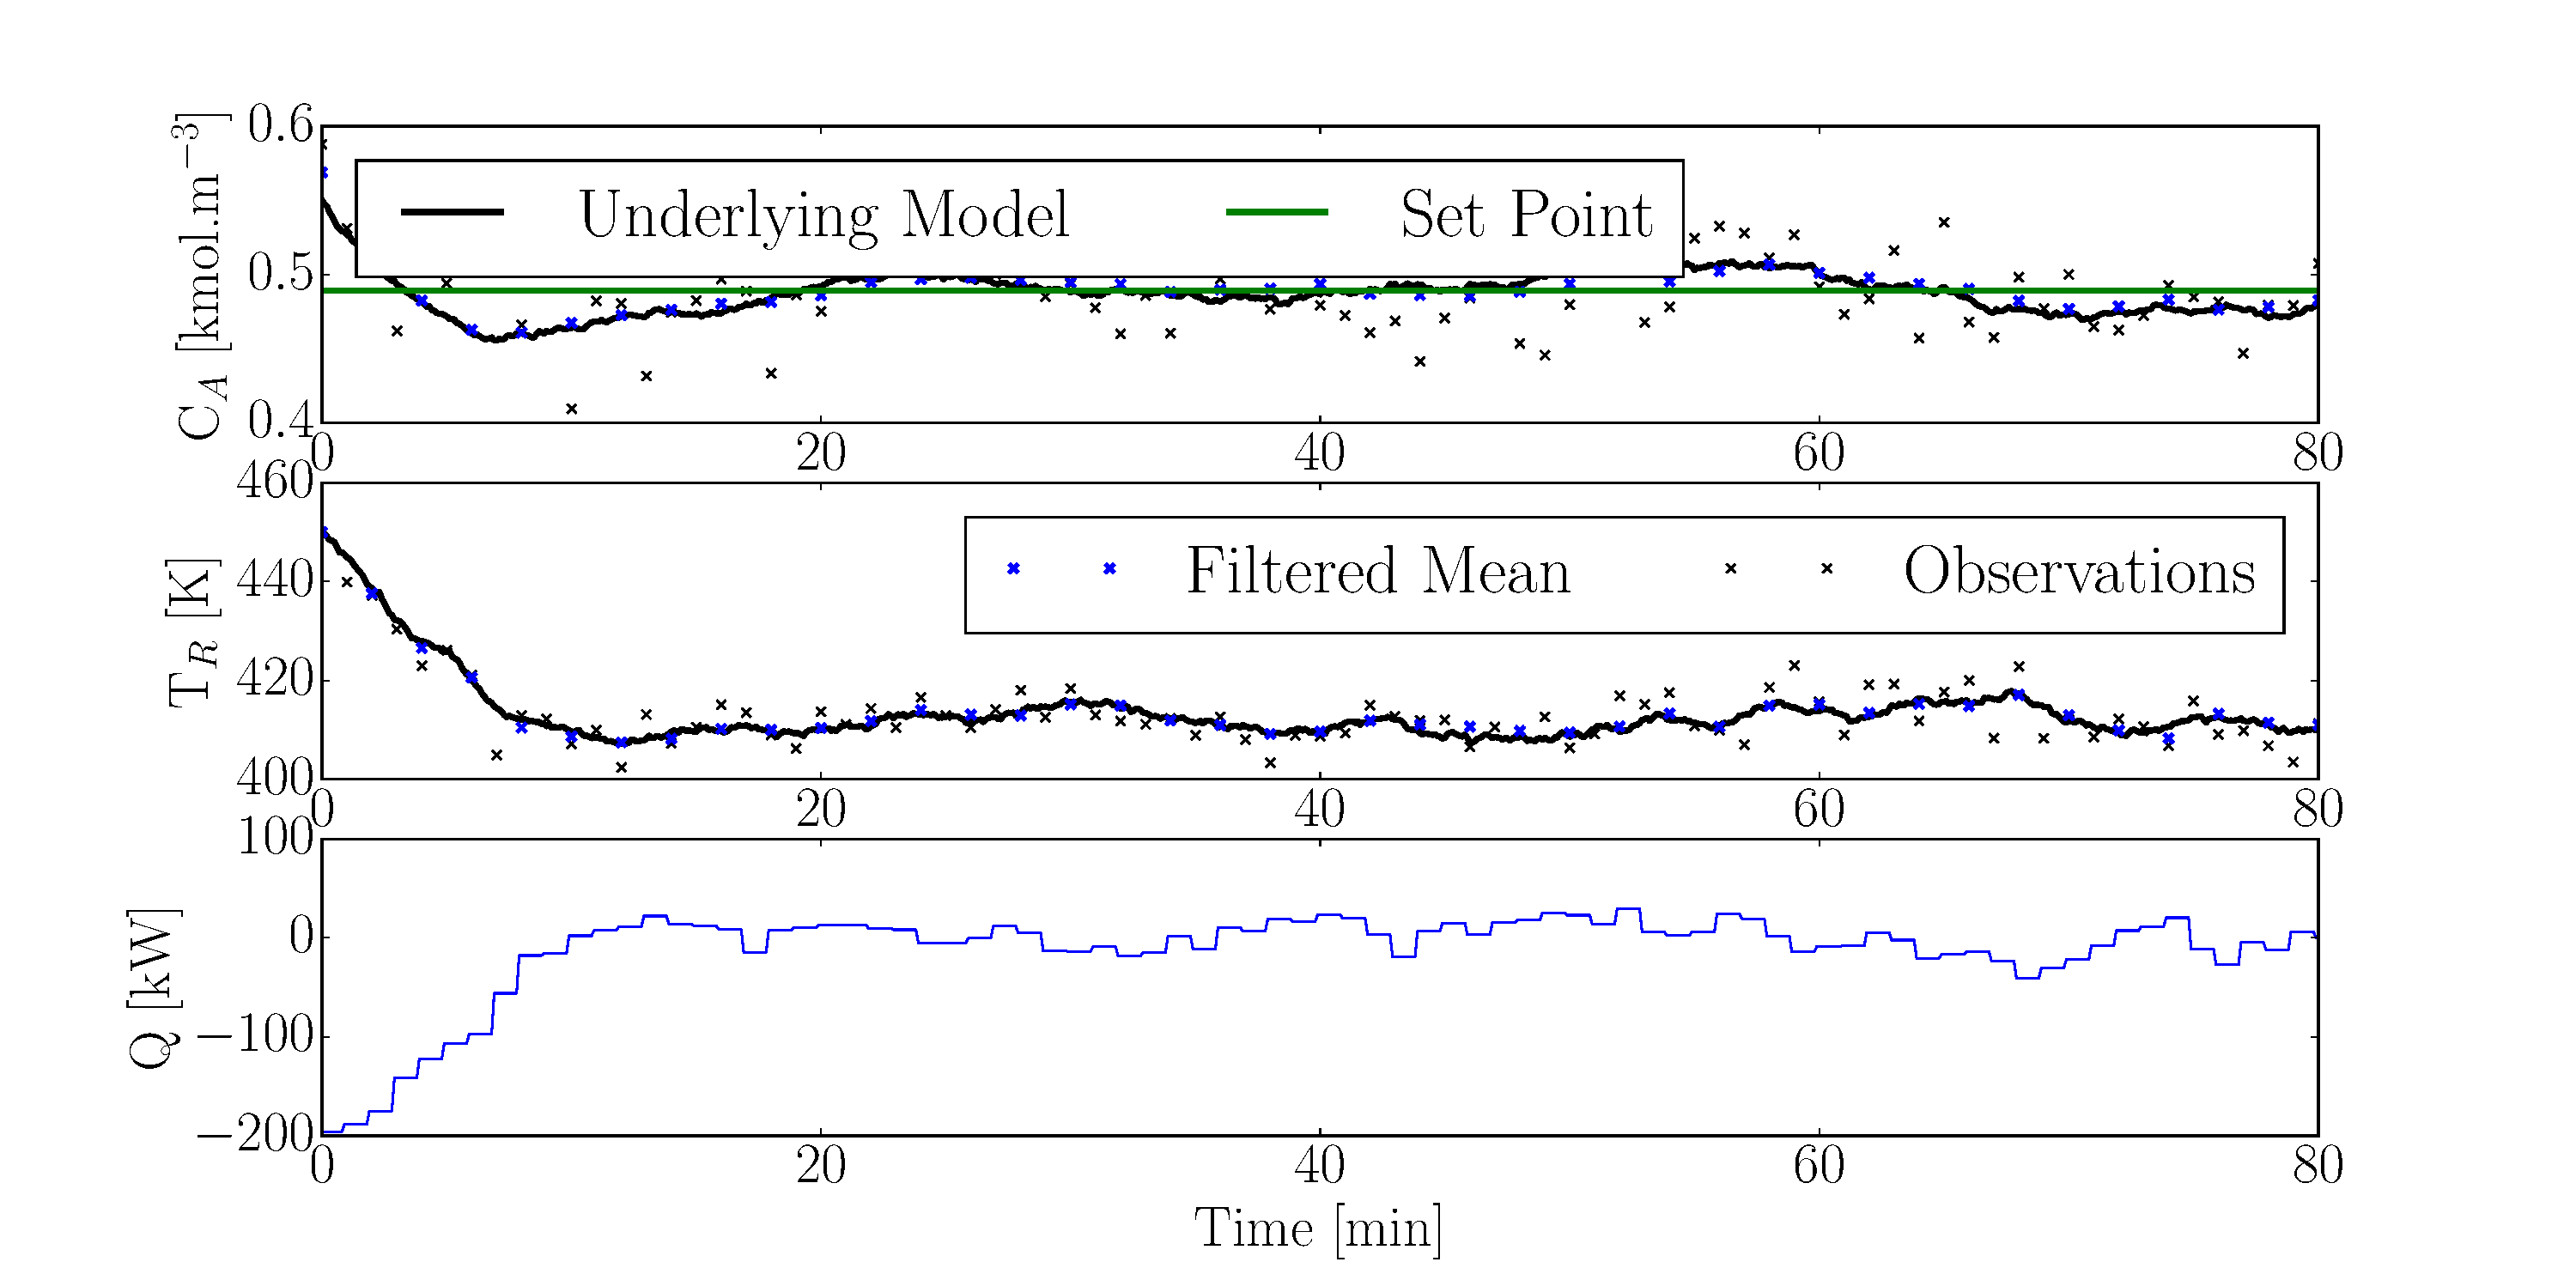
\includegraphics[scale=0.25]{lin_mod_lqg.pdf}
\caption{Unconstrained LQG regulator tracking with initial condition $(0.55, 450)$ and measuring both states.}
\label{fig_lin_mod_lqg}
\end{figure}
The average heat energy usage (controller input) over the simulation run is 214 kJ/min. The average set point error is 2.38\% over the same 40 min time period\footnote{We define the average energy input by $\frac{h}{N}\sum^N_{t=0}|u_t-u_s|$ and the average concentration error by $\frac{1}{N}\sum^N_{t=0}|\frac{{C_A}_t-y_{sp}}{y_{sp}}|$}.
 
Next we illustrate the approach of using conventional deterministic MPC to control the stochastic system. The MPC formulation is shown in (\ref{eq_mpc_constrained_det1}). Using MPC allows us to easily add state and input constraints; this is a significant improvement over conventional LQG as discussed previously.
\begin{equation}
\begin{aligned}
&\underset{\mathbf{u}}{\text{min }} \frac{1}{2}\sum_{k=0}^{N-1} \left( \mu_k^TQ\mu_k + u_k^TRu_k \right) + \frac{1}{2}\mu_N^TP_f\mu_N \\
& \text{subject to } \mu_{t+1}=A\mu_t + Bu_t \\
&\text{and } \begin{pmatrix}
10 \\ 1
\end{pmatrix}^T \mu_t + 411 \geq 0 ~\forall ~t=1,...,N\\
& \text{and } |u_t| \leq 10000 ~\forall ~t=0,...,N-1\\
\end{aligned}
\label{eq_mpc_constrained_det1}
\end{equation}
We only use a single state constraint in this dissertation but the extension to multiple constraints is straightforward. The prediction and control horizon are equal to each other and set at 150 time steps i.e. 15 minutes into the future. We additionally constrain the magnitude of the inputs.

Since we have assumed normality the deterministic state inequality constraint can also be seen as an affine expected value constraint as shown in Theorem \ref{thrm_affine_expected_const}.

In Figure \ref{fig_lin_mod_kf_mean_track} we see the reference tracking and controller input for the deterministic MPC. The average heat energy input and set point error over the simulation run is 2.70\% and 222 kJ/min. Interestingly the average error is not much different but the controller requires more energy to track the setpoint without violating the constraints. This is reasonable because the additional constraints make problem (\ref{eq_mpc_constrained_det1}) a harder problem than (\ref{eq_lqg_linmod}).
\begin{figure}[H] 
\centering
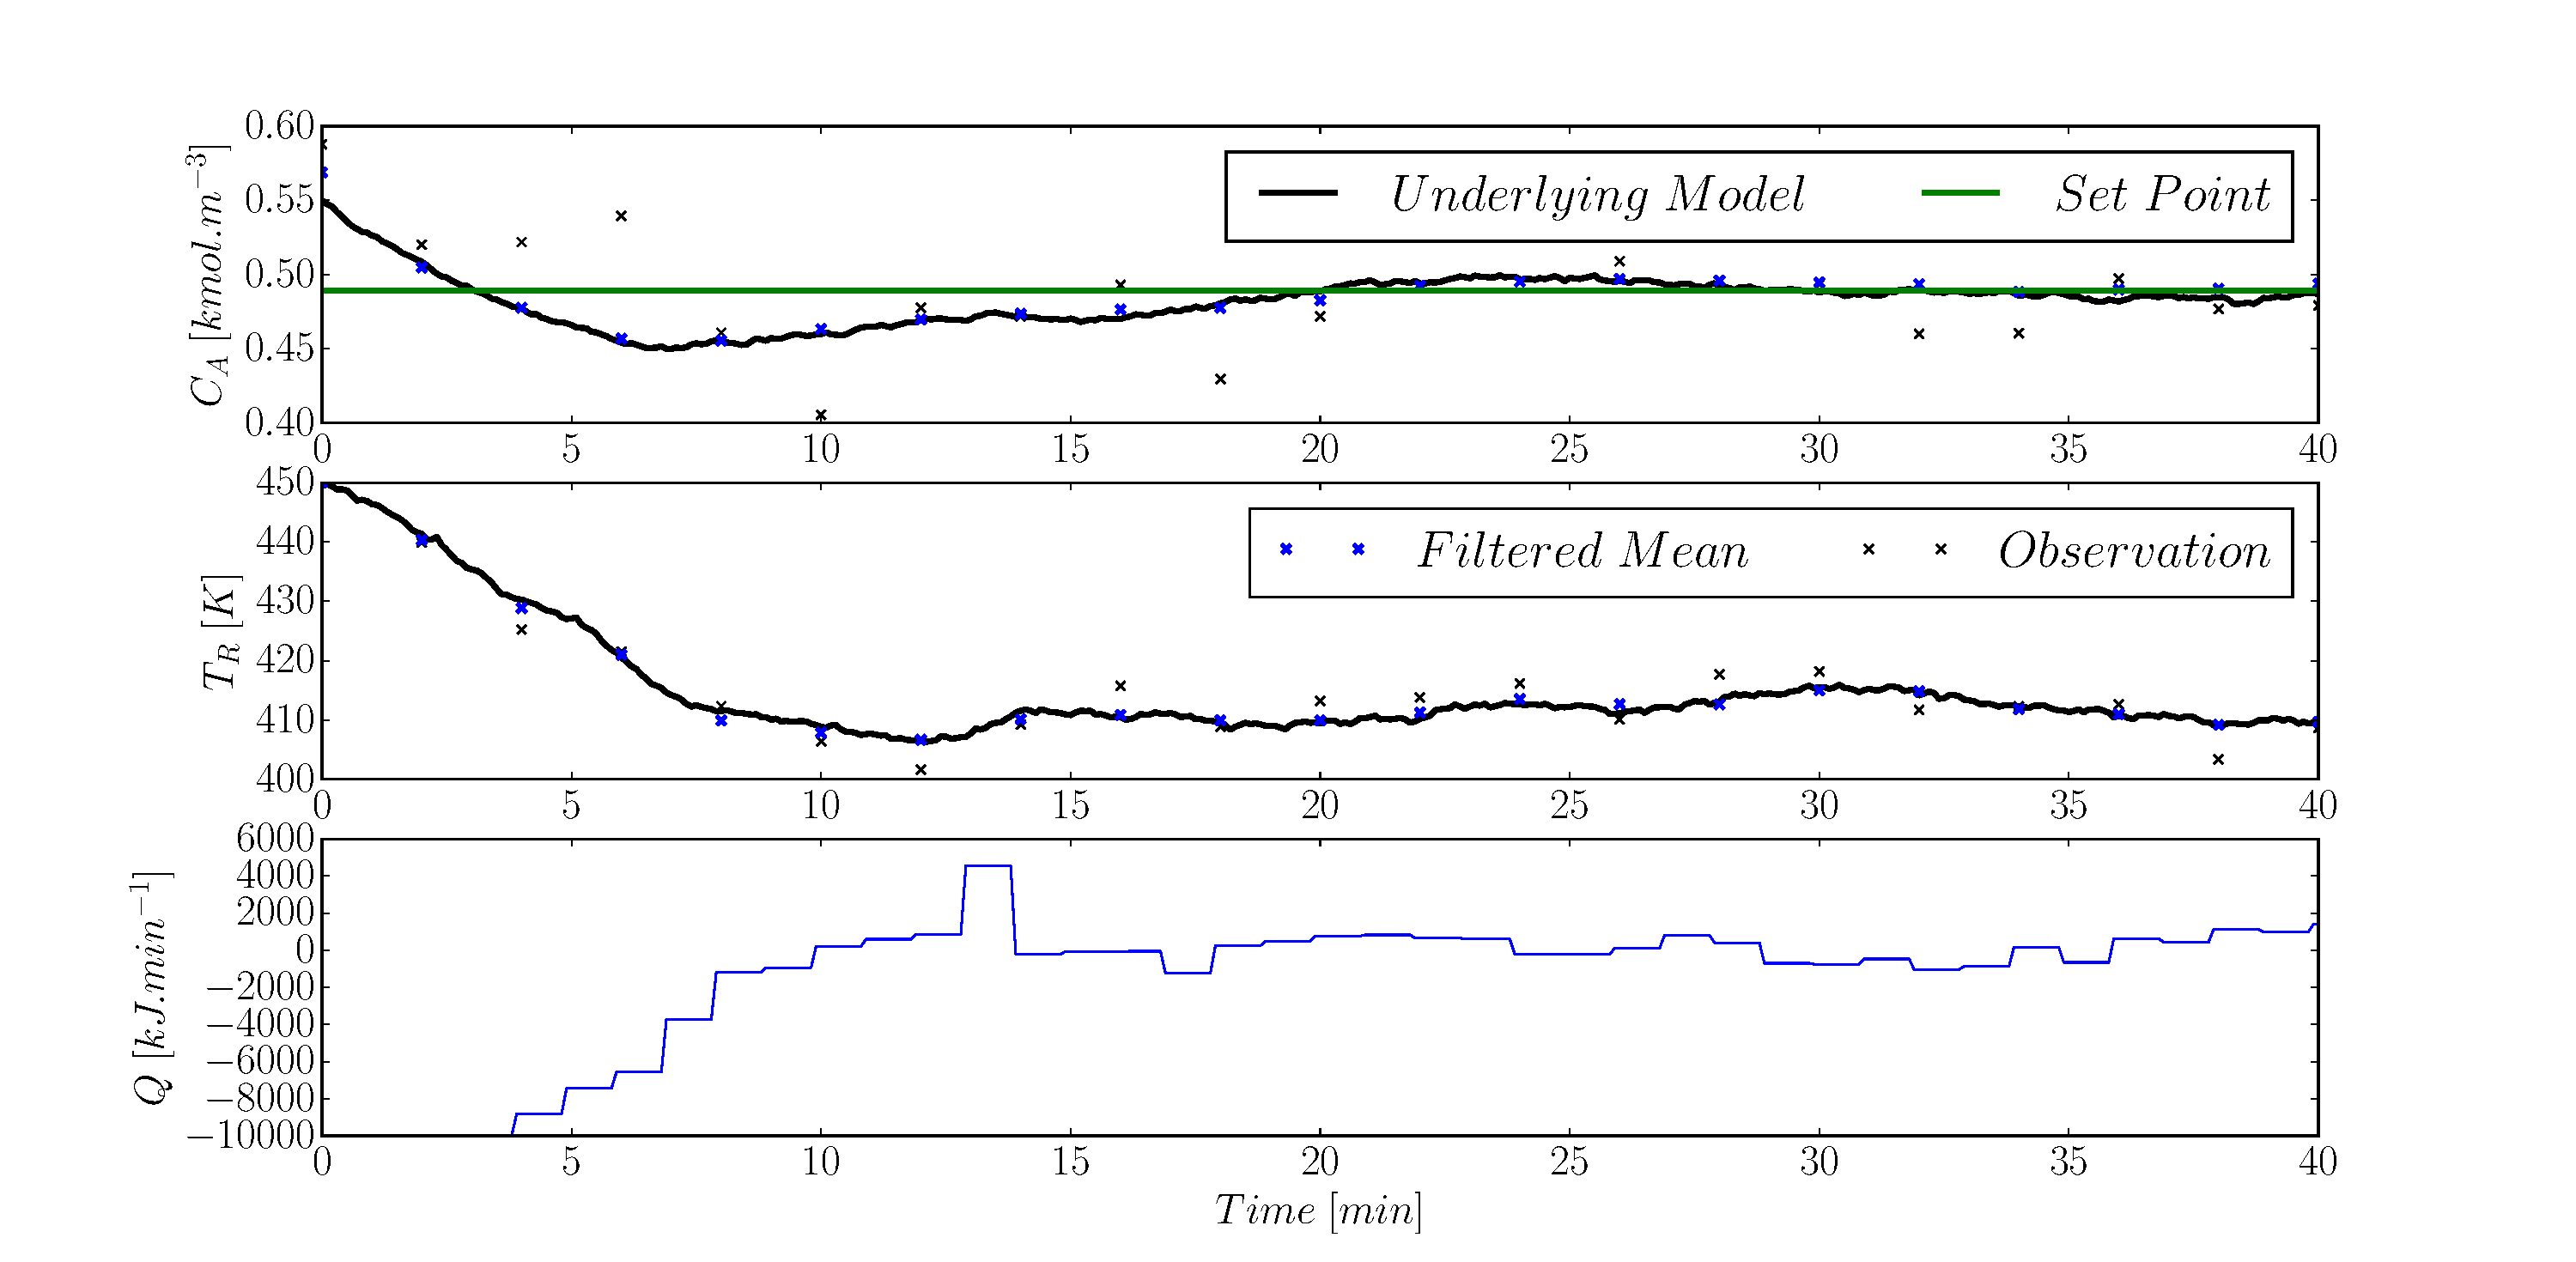
\includegraphics[scale=0.25]{lin_mod_kf_mean_track.pdf}
\caption{Deterministic constrained MPC tracking with initial condition $(0.55, 450)$ and measuring both states.}
\label{fig_lin_mod_kf_mean_track}
\end{figure}
Like the LQG controller, it is clear that we have noisy convergence to the set point. As mentioned previously we will never be able to achieve zero set point offset because of the noise term in the system dynamics (\ref{eq_lin_system}). Note that we have constrained the maximum magnitude of the inputs such that $|u_t| \leq 10000$ kJ/min. In the unconstrained case the controller required a maximum absolute input magnitude of over $12000$ kJ/min; the ability to naturally constrain the input can be practically very useful. The benefit of MPC is apparent here.

In Figure \ref{fig_lin_mod_kf_mean_ss} we see the corresponding state space trajectory of the system together with the state constraint.
\begin{figure}[H] 
\centering
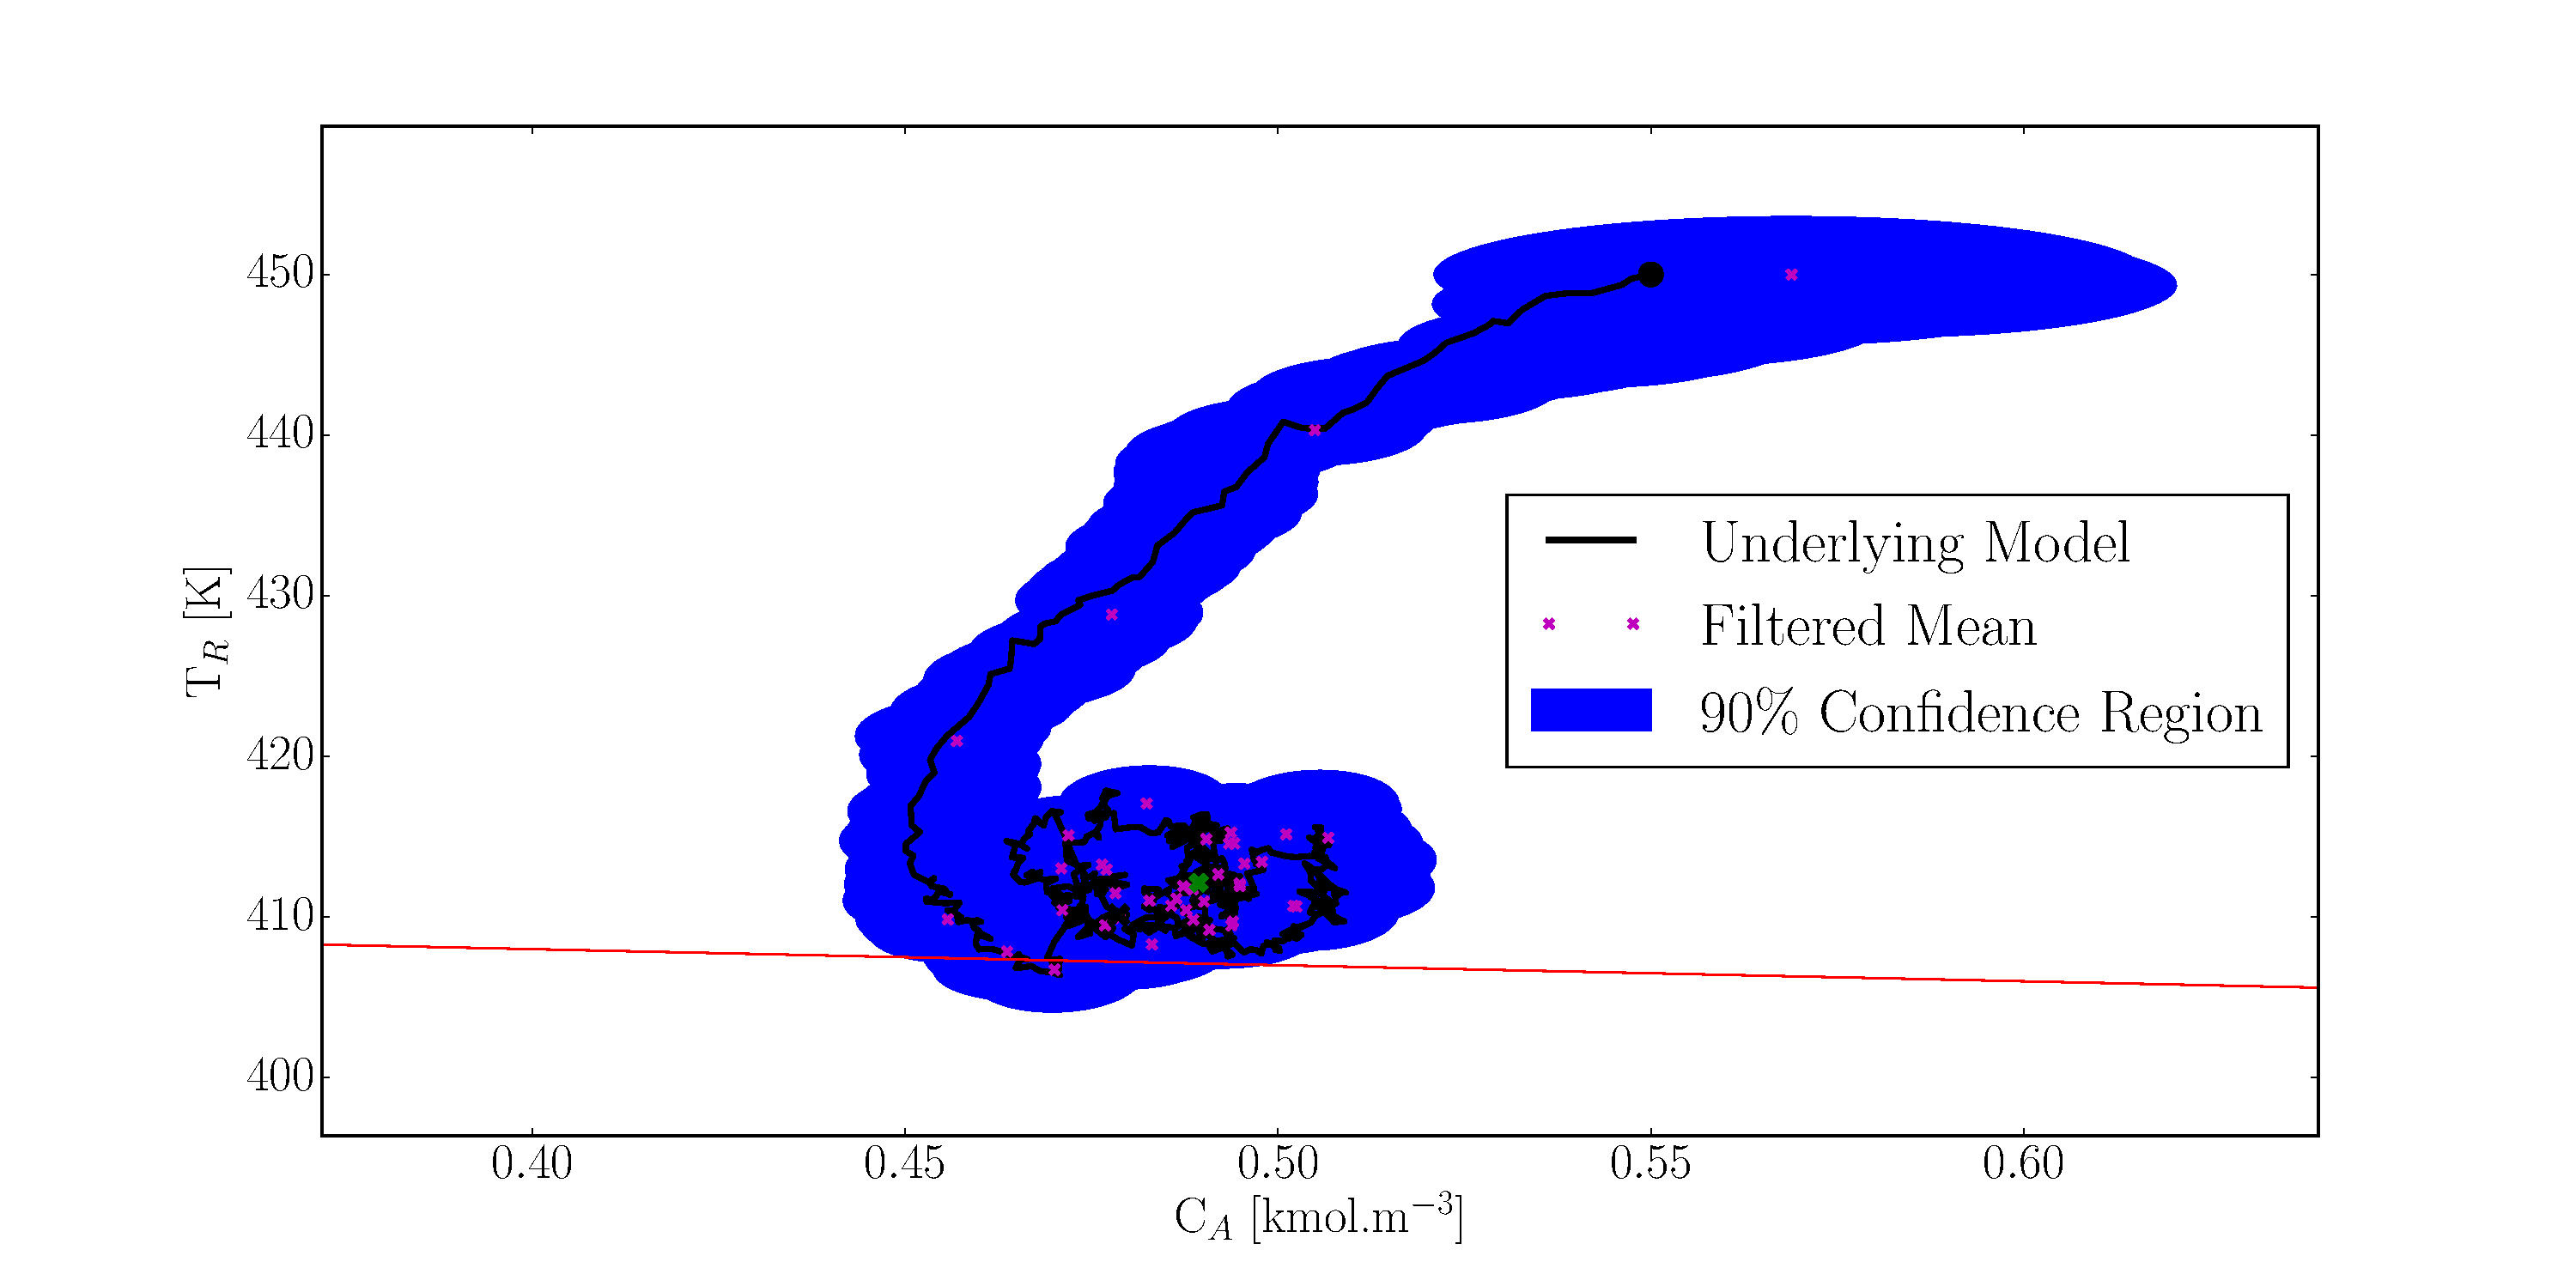
\includegraphics[scale=0.25]{lin_mod_kf_mean_ss.pdf}
\caption{Deterministic MPC state space trajectory with initial condition $(0.55, 450)$ and measuring both states.}
\label{fig_lin_mod_kf_mean_ss}
\end{figure}
While the predicted mean state estimates do not violate the constraint (due to the optimisation constraints) the actual underlying system does.  This is clearly seen if one inspects the confidence region around the lower state estimates. The confidence region is deeply violated by the constraint which implies that it is likely that the underlying system might. This is clearly a problem from a control point of view; the deterministic MPC cannot ensure that the constraint is satisfied.

We remedy this situation by introducing the stochastic MPC as discussed in Theorem \ref{thrm_mpc_stoch_to_det} and shown in (\ref{eq_mpc_linmod_kf_cons}) for convenience. Note that $d^T = (10, 1)$ and $e=411$ as before. By consulting a Chi-Squared Distribution table we set $k^2 = 4.6052$ which corresponds to the chance constraint $\text{Pr}(d^Tx_t + e \geq 0) \geq 90\% ~\forall ~t=1,...,N$.
\begin{equation}
\begin{aligned}
&\underset{\mathbf{u}}{\text{min }} \frac{1}{2}\sum_{k=0}^{N-1} \left( \mu_k^TQ\mu_k + u_k^TRu_k \right) + \frac{1}{2}\mu_N^TP_f\mu_N + \frac{1}{2}\sum_{k=0}^N \text{tr}(Q\Sigma_k) \\
& \text{subject to } \mu_{t+1}=A\mu_t + Bu_t \\
& \text{and } \Sigma_{t+1} = W+A\Sigma_t A^T \\
& \text{and } d^T\mu_t + e \geq k\sqrt{d^T \Sigma_t d} ~\forall ~t=1,...,N\\
& \text{and } |u_t| \leq 10000 ~\forall ~t=0,...,N-1\\
\end{aligned}
\label{eq_mpc_linmod_kf_cons}
\end{equation}
Note that problem (\ref{eq_mpc_linmod_kf_cons}) is harder than (\ref{eq_mpc_constrained_det1}) due to the added constraint and thus we expect that the system will require greater controller input to satisfy the constraint. 

In Figure \ref{fig_lin_mod_kf_var90_track} we see that the stochastic MPC is able to track the set point in a similar manner as the LQG controller and deterministic MPC. The total average heat input and set point error over the simulation run is 290 kJ/min and 2.95\% respectively. This problem is harder than the preceding one due to the additional constraint and thus more energy is required. 
\begin{figure}[H] 
\centering
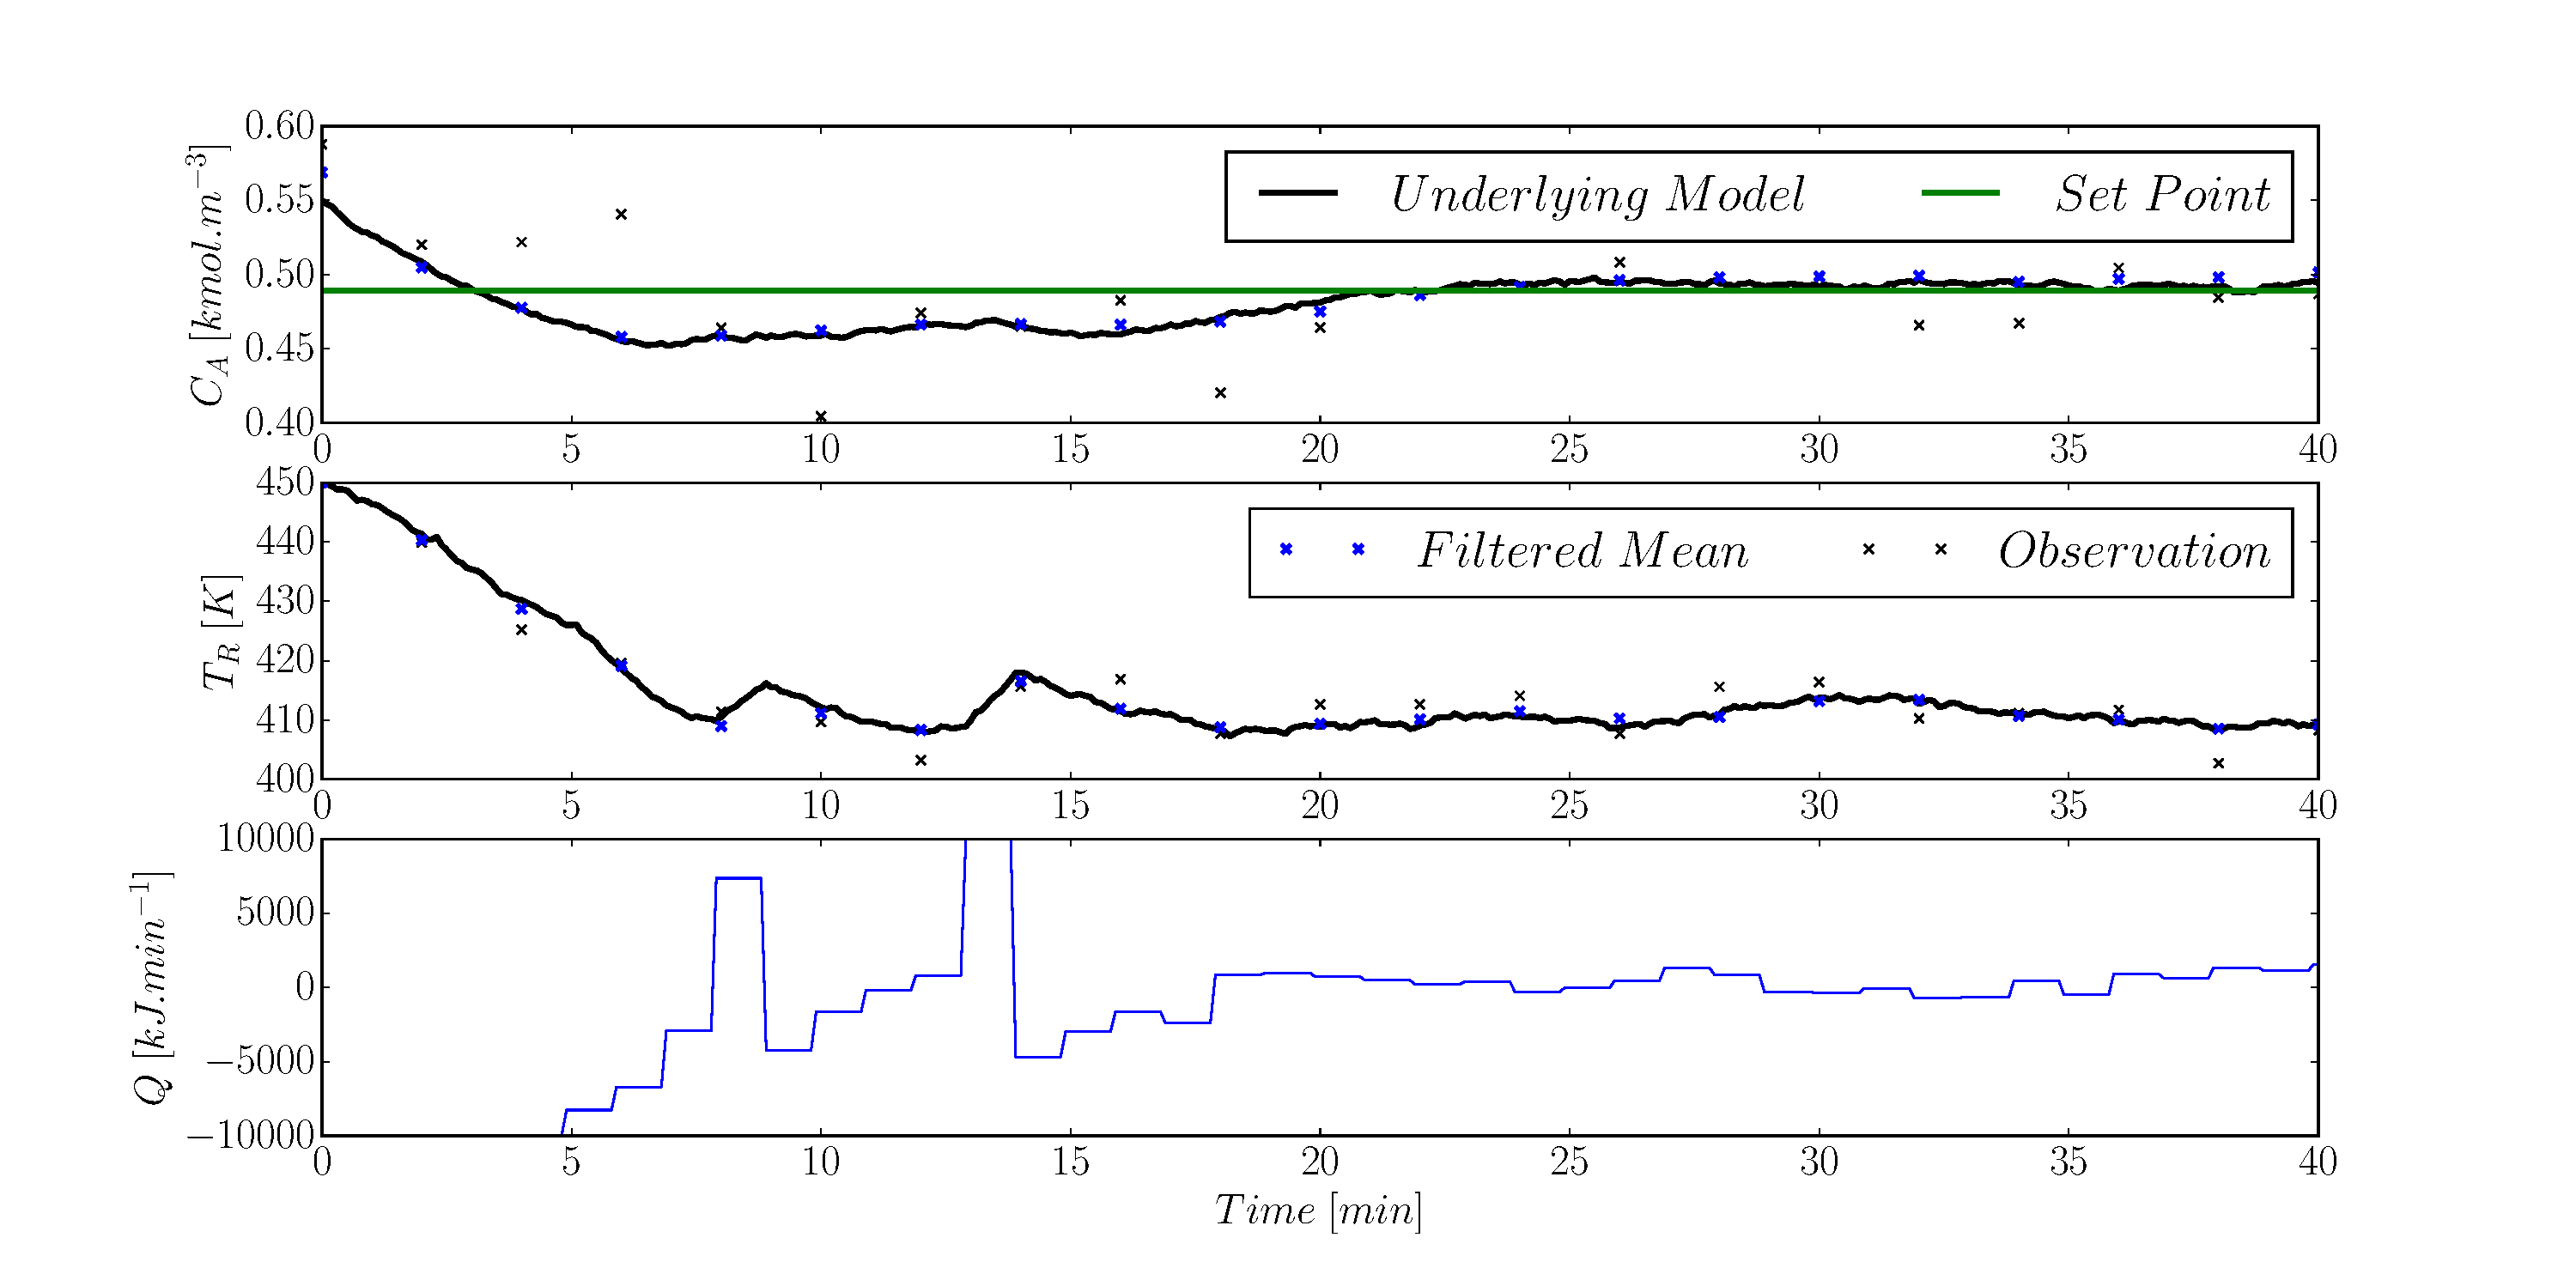
\includegraphics[scale=0.25]{lin_mod_kf_var90_track.pdf}
\caption{Stochastic constrained MPC tracking with initial condition $(0.55, 450)$ and measuring both states. A Kalman Filter is used for inference and the chance constraint is set at 90\%.}
\label{fig_lin_mod_kf_var90_track}
\end{figure}
However, the benefit of adding the stochastic constraint is apparent in Figure \ref{fig_lin_mod_kf_var90_ss}. It is clear that the constraint on the underlying state is not violated.
\begin{figure}[H] 
\centering
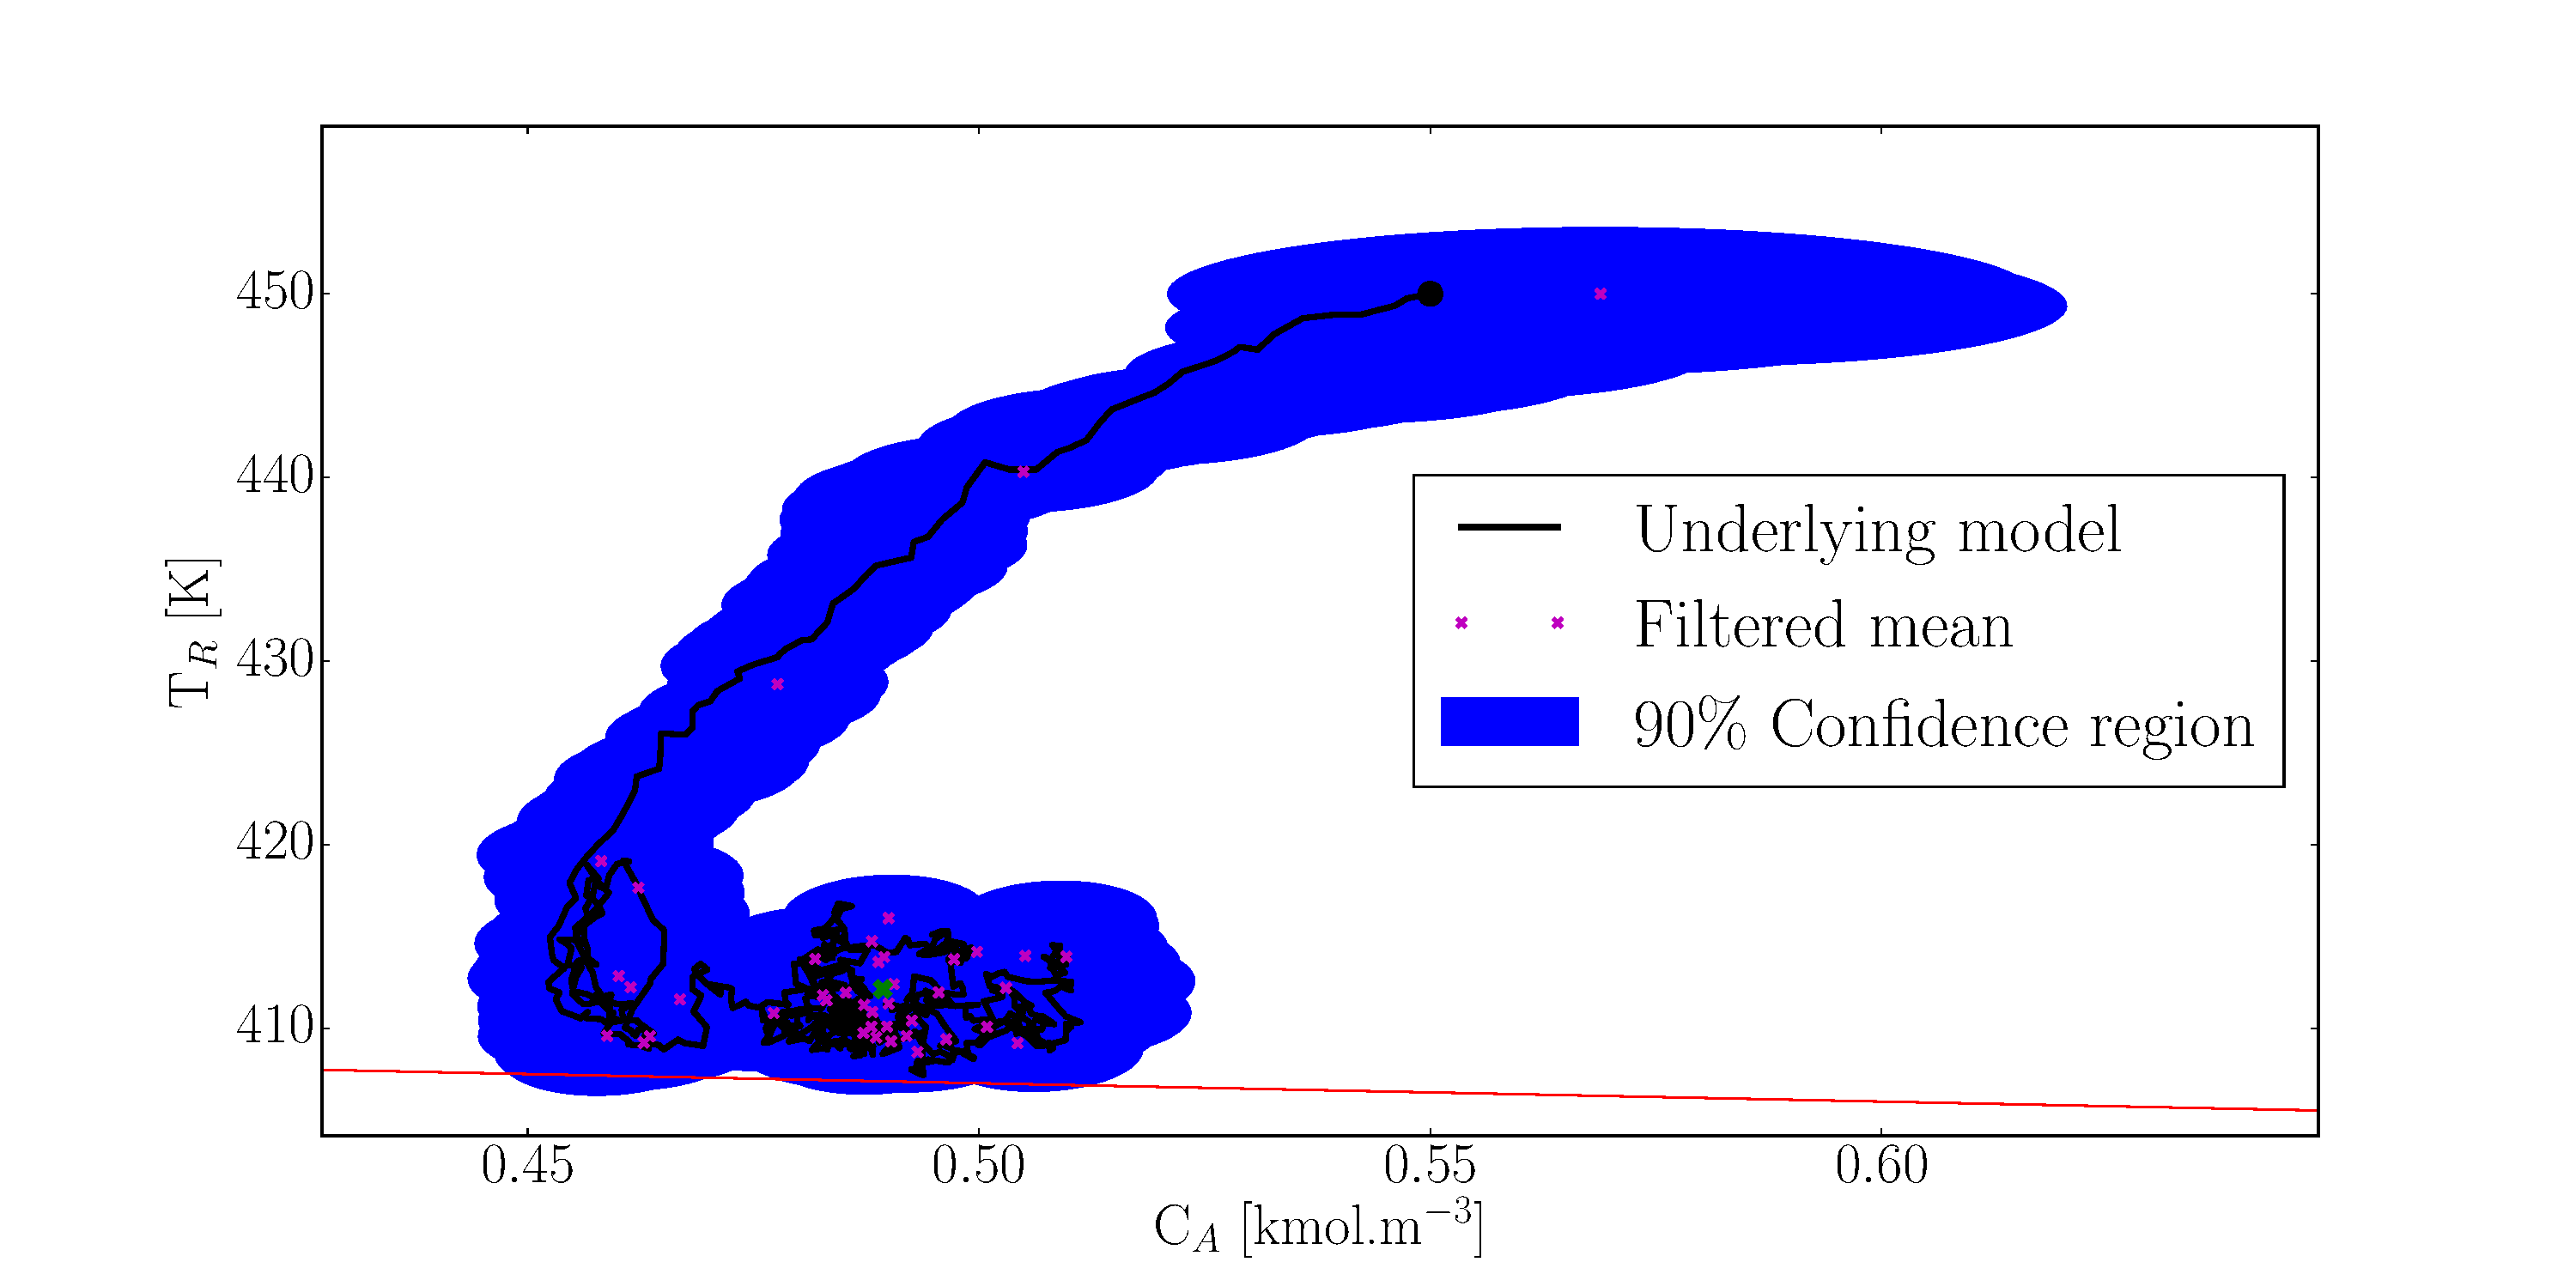
\includegraphics[scale=0.25]{lin_mod_kf_var90_ss.pdf}
\caption{Stochastic constrained MPC state space trajectory with initial condition $(0.55, 450)$ and measuring both states. A Kalman Filter is used for inference and the chance constraint is set at 90\%.}
\label{fig_lin_mod_kf_var90_ss}
\end{figure}
Since the stochastic constraint is only enforced with probability 90\% it is possible that the underlying system can come ``close" to the constraint. This then has the consequence that the posterior confidence region marginally violates (spills over) the constraint as seen in the lower regions of Figure \ref{fig_lin_mod_kf_var90_ss}.

It is interesting to investigate what effect increasing the probability that the chance constraint is satisfied will have on the system. To this end we modify the chance constraint of (\ref{eq_mpc_linmod_kf_cons}) such that $k^2 = 13.8155$ which corresponds to the chance constraint $\text{Pr}(d^Tx_t + e \geq 0) \geq 99.9\% ~\forall ~t=1,...,N$. We expect that the underlying system will be moved further away from constraint due to this added level of conservativeness.

In Figure \ref{fig_lin_mod_kf_var999_track} we see that the stochastic MPC still tracks the set point and Figure \ref{fig_lin_mod_kf_var999_ss} shows that the expected behaviour is realised. 
\begin{figure}[H] 
\centering
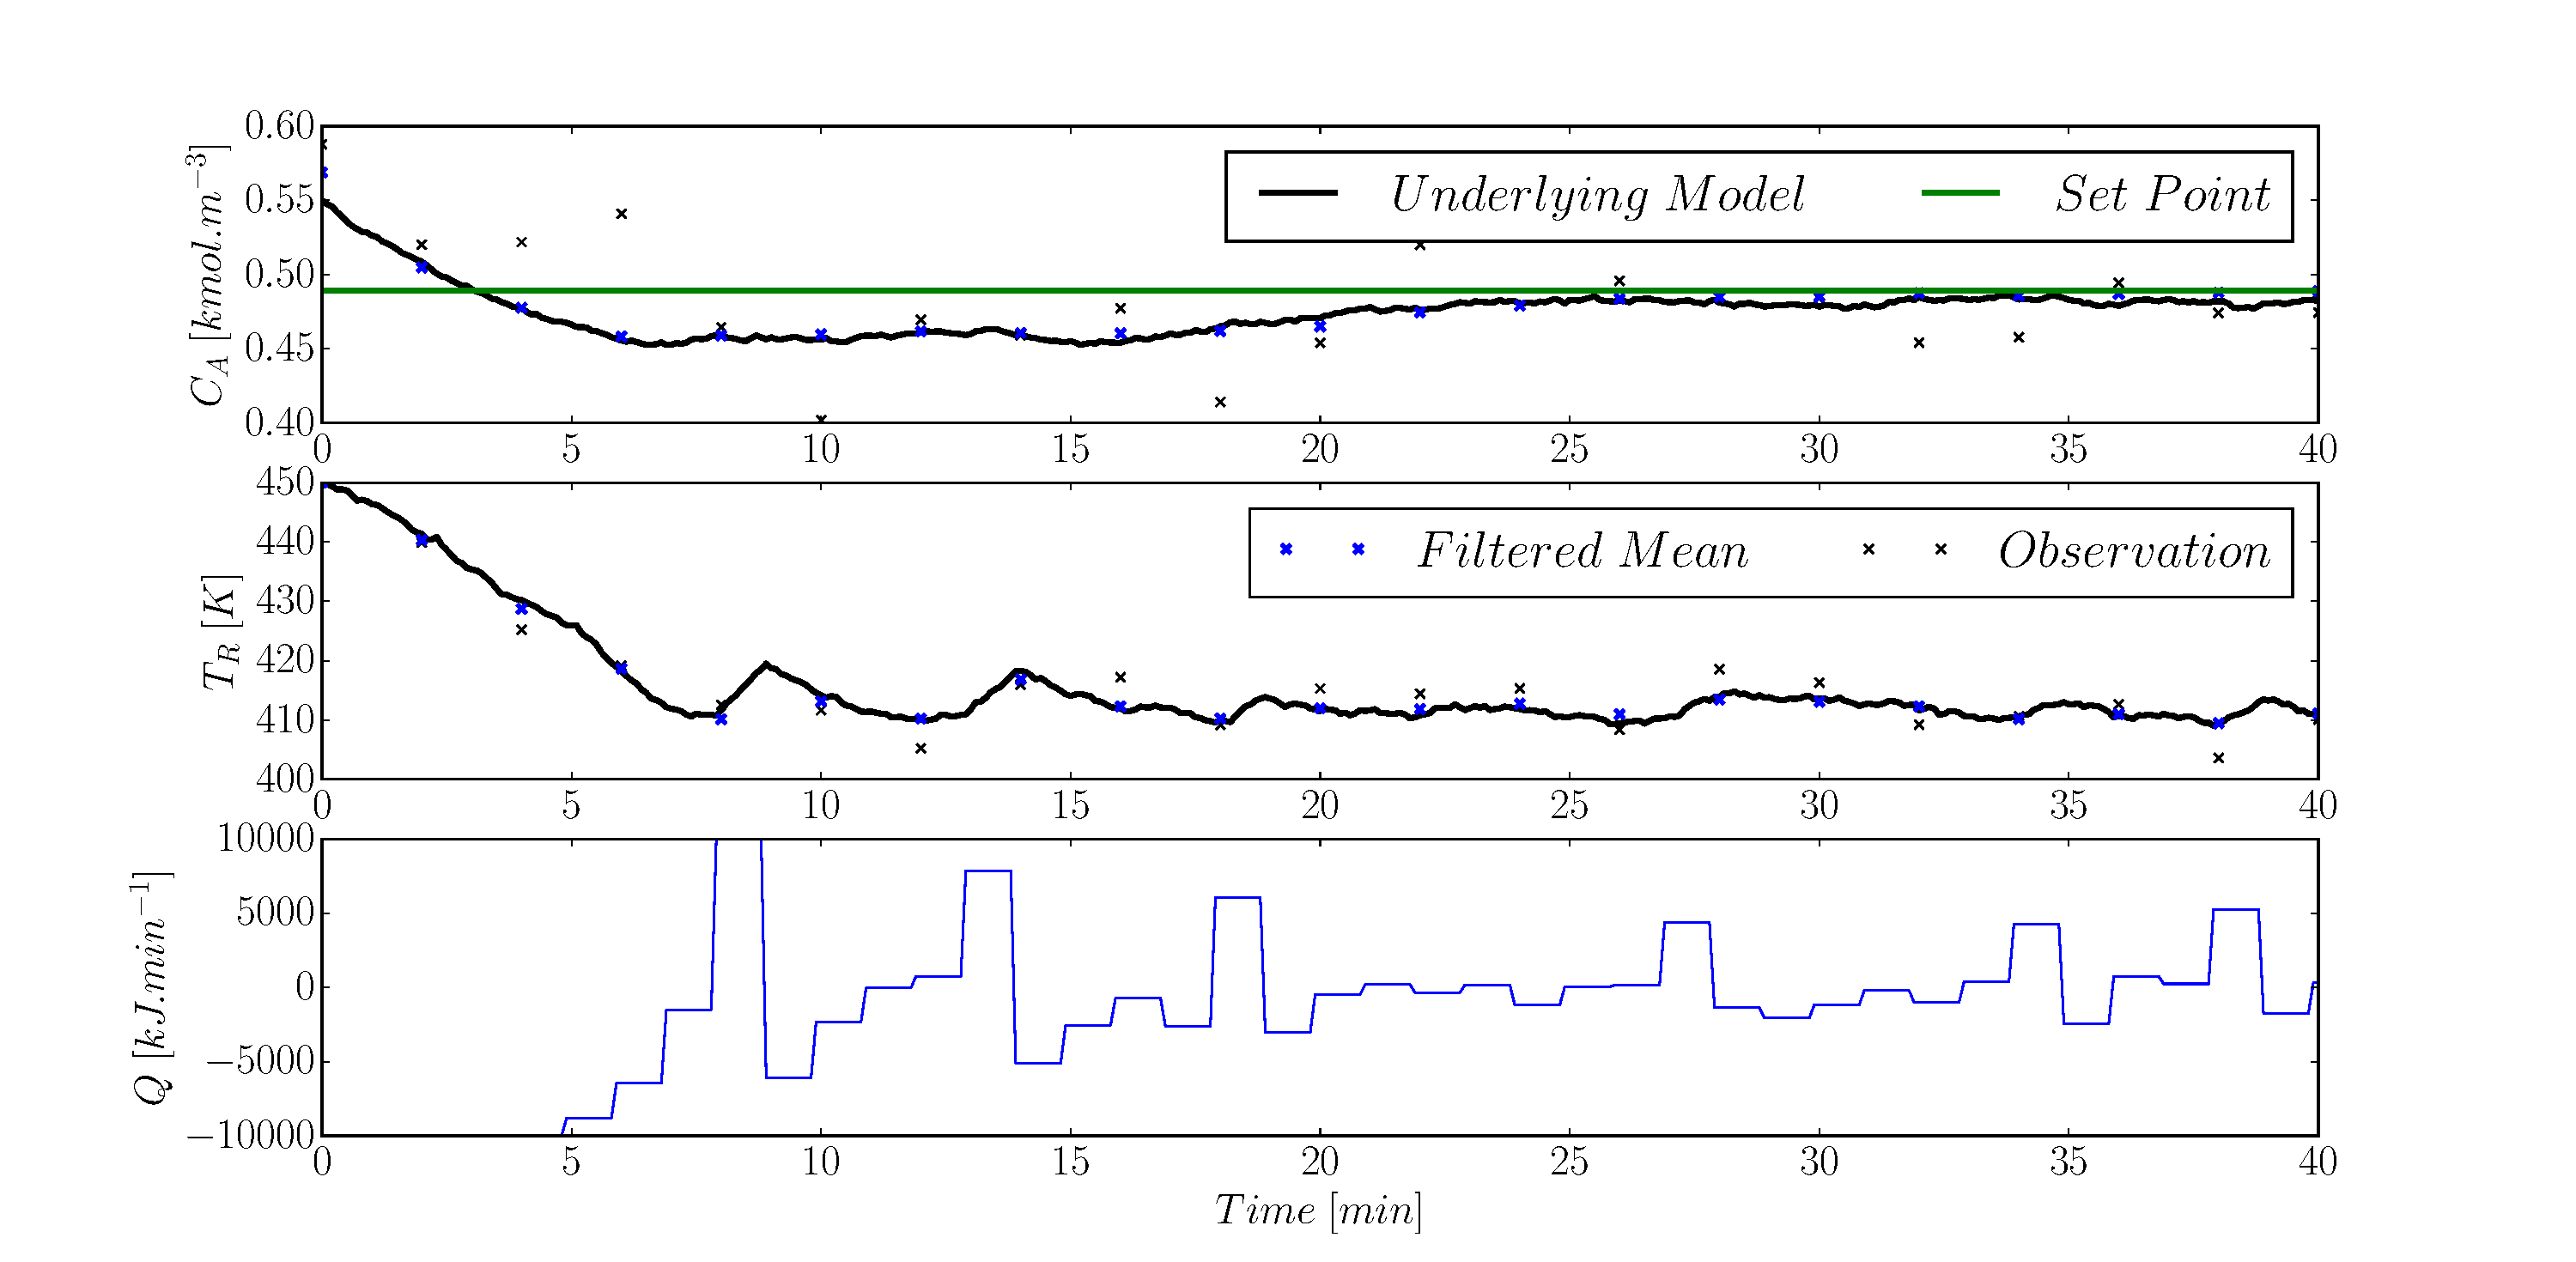
\includegraphics[scale=0.25]{lin_mod_kf_var999_track.pdf}
\caption{Stochastic constrained MPC tracking with initial condition $(0.55, 450)$ and measuring both states. A Kalman Filter is used for inference and the chance constraint is set at 99.9\%.}
\label{fig_lin_mod_kf_var999_track}
\end{figure}
The average heat input and average set point error is 3.73\% and 351 kJ/min. The added conservativeness of the MPC prevents it from attempting to get to the set point as fast as the previous stochastic MPC; this causes the higher average error but the constraints are satisfied more robustly. As before, the control problem is harder and thus requires more energy.

In Figure \ref{fig_lin_mod_kf_var999_ss} we see the 90\% confidence region is above the constraint. Since the probability that the predicted states are close to the constraint is much lower than before we see that the confidence region satisfies the constraint everywhere.
\begin{figure}[H] 
\centering
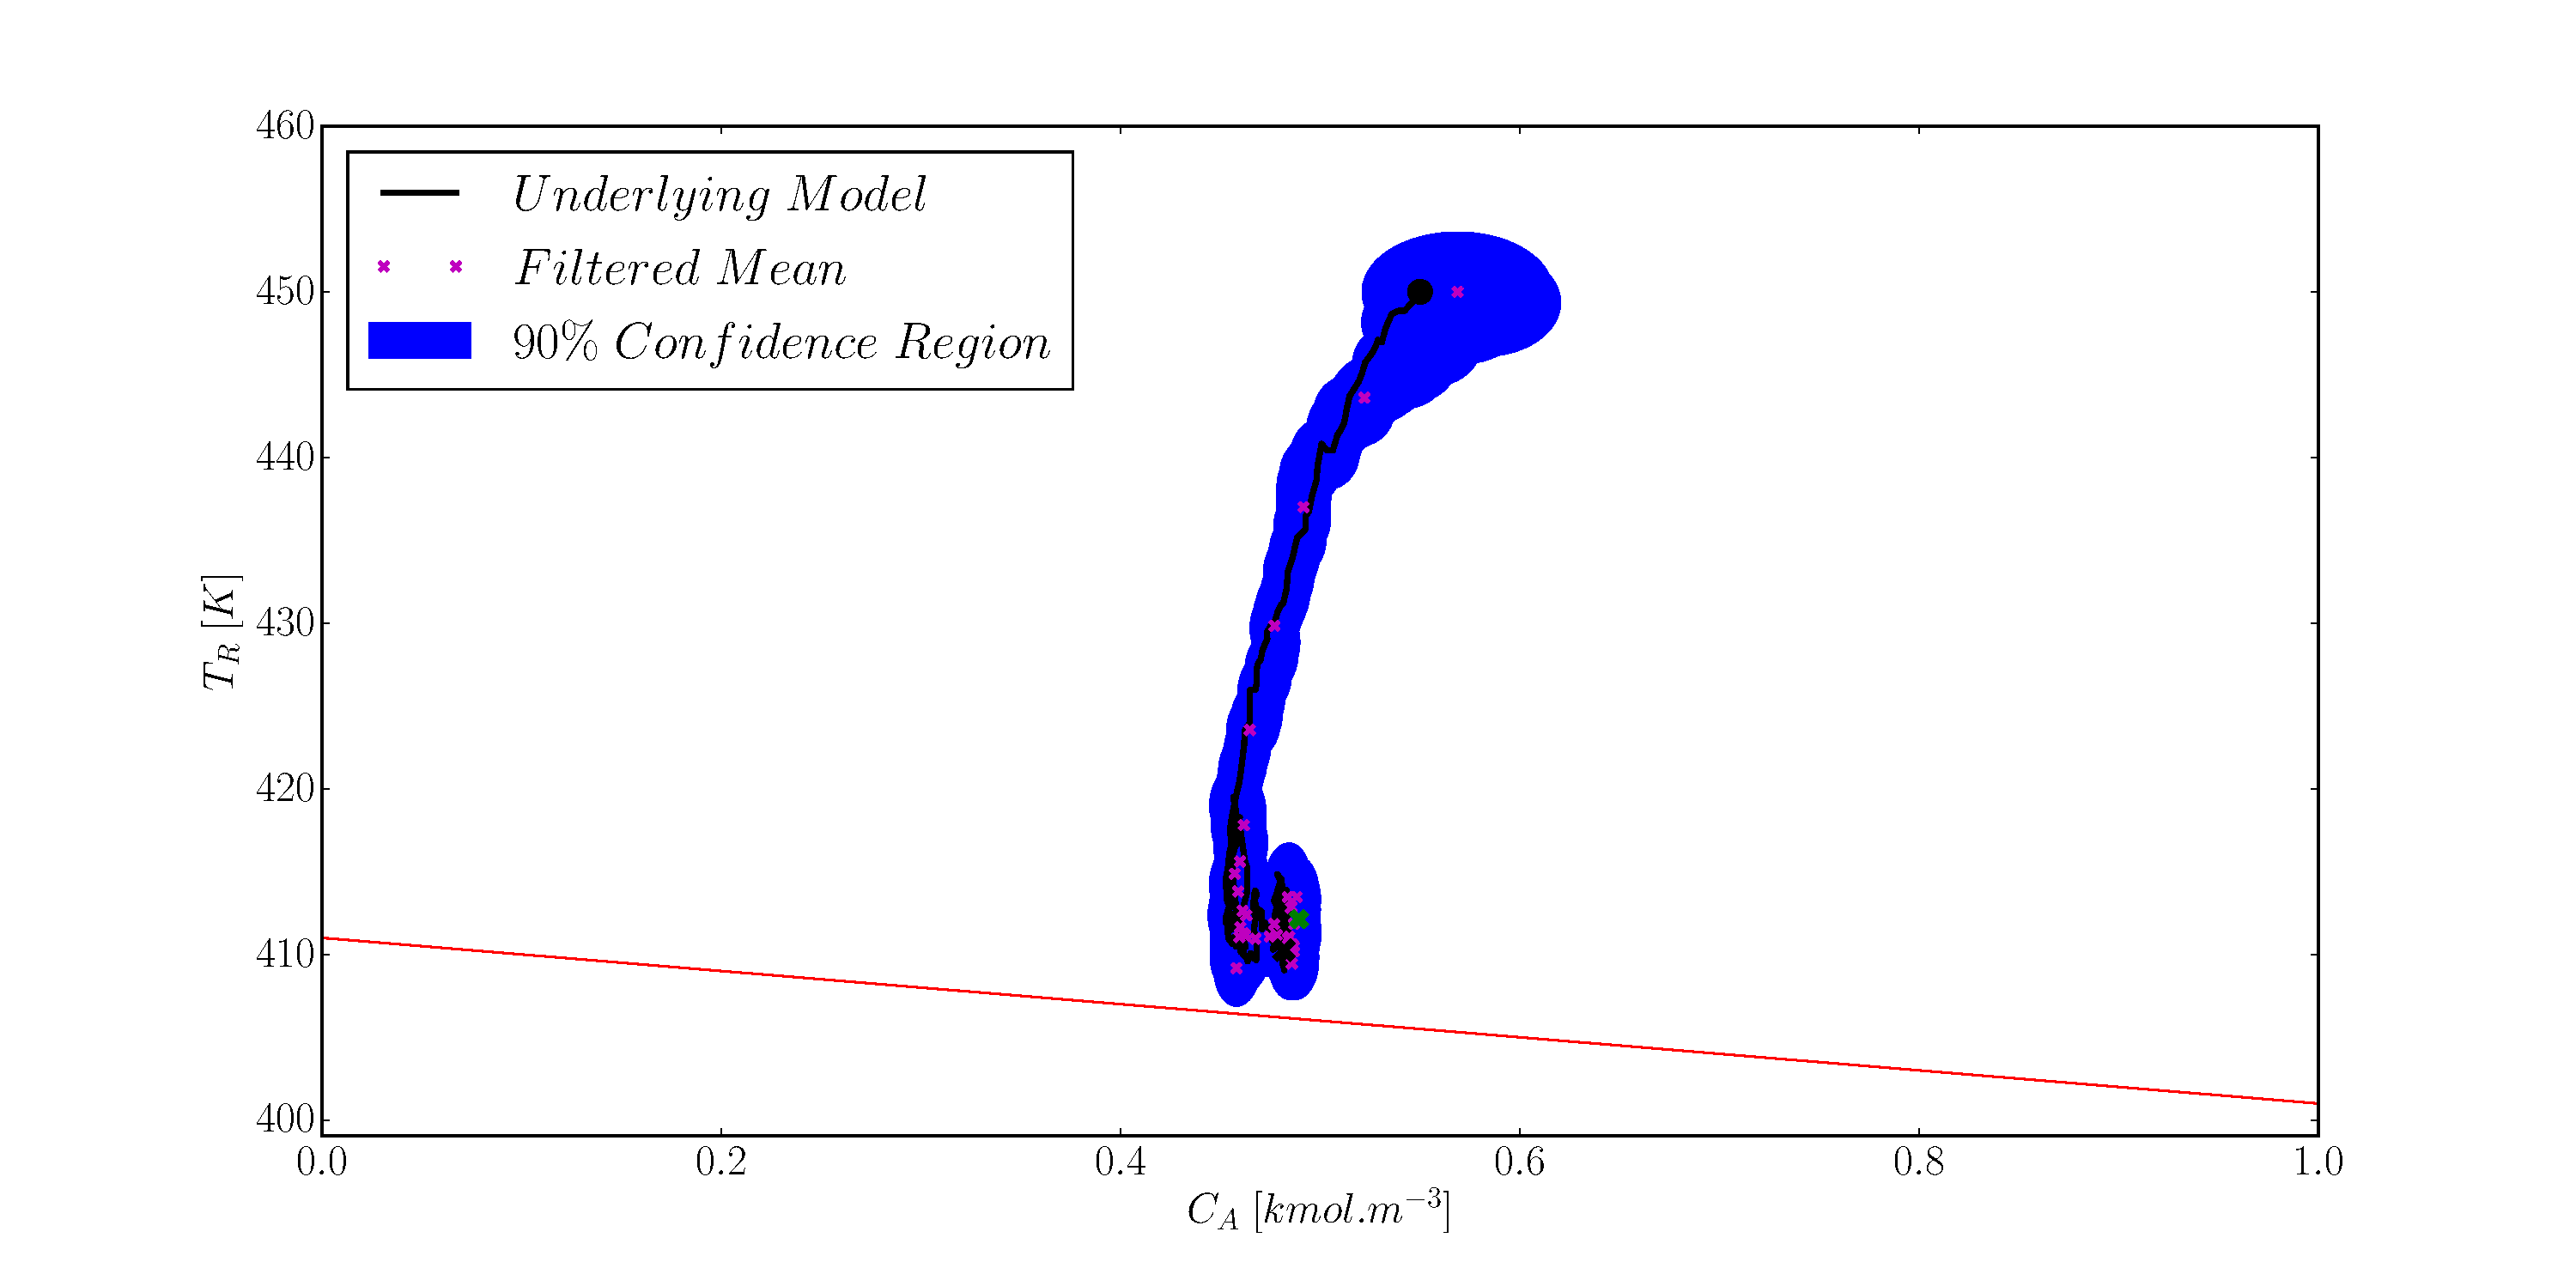
\includegraphics[scale=0.25]{lin_mod_kf_var999_ss.pdf}
\caption{Stochastic constrained MPC state space trajectory with initial condition $(0.55, 450)$ and measuring both states. A Kalman Filter is used for inference and the chance constraint is set at 99.9\%.}
\label{fig_lin_mod_kf_var999_ss}
\end{figure}
It would also be correct to infer that $k$ can be used as an empirical measure of the inherent stochastic conservativeness of the resulting controller. That is, lower values of $k$ indicate a more aggressive controller which may violate the chance constraints and higher values of $k$ indicate a more conservative controller. This can be useful for systems where the normal assumption is not valid but one would still like to enforce stochastic constraints in some empirical sense. 

We have made the strong assumption that the system dynamics remain linear and Gaussian even under the MPC control law which is not necessarily linear \cite{mac}. Clearly if the system is far from Gaussian the Gaussian approach to simplifying the chance constraint will not be valid. Fortunately this is relatively simple to check and serves as a good way of measuring controller health. That is, the more Gaussian the filtered distributions are, the better the linear stochastic controller will work. 

Kullback-Leibler Divergence was introduced in Theorem \ref{thrm_kl_sample} to estimate the degree to which samples match a given distribution. From Section \ref{sec_inf_nonlin_mods} we know that given enough particles a Particle Filter can accurately represent any distribution. Thus we temporarily replace the Kalman Filter with a Particle filter and use Theorem \ref{thrm_kl_sample} to estimate the degree of normality of the posterior state distributions.

Figure \ref{fig_lin_mod_kl} shows the degree to which the underlying distribution is Gaussian. Since we cannot use an infinite amount of particles we compare the sampled Gaussian distribution approximation to a baseline.   
\begin{figure}[H] 
\centering
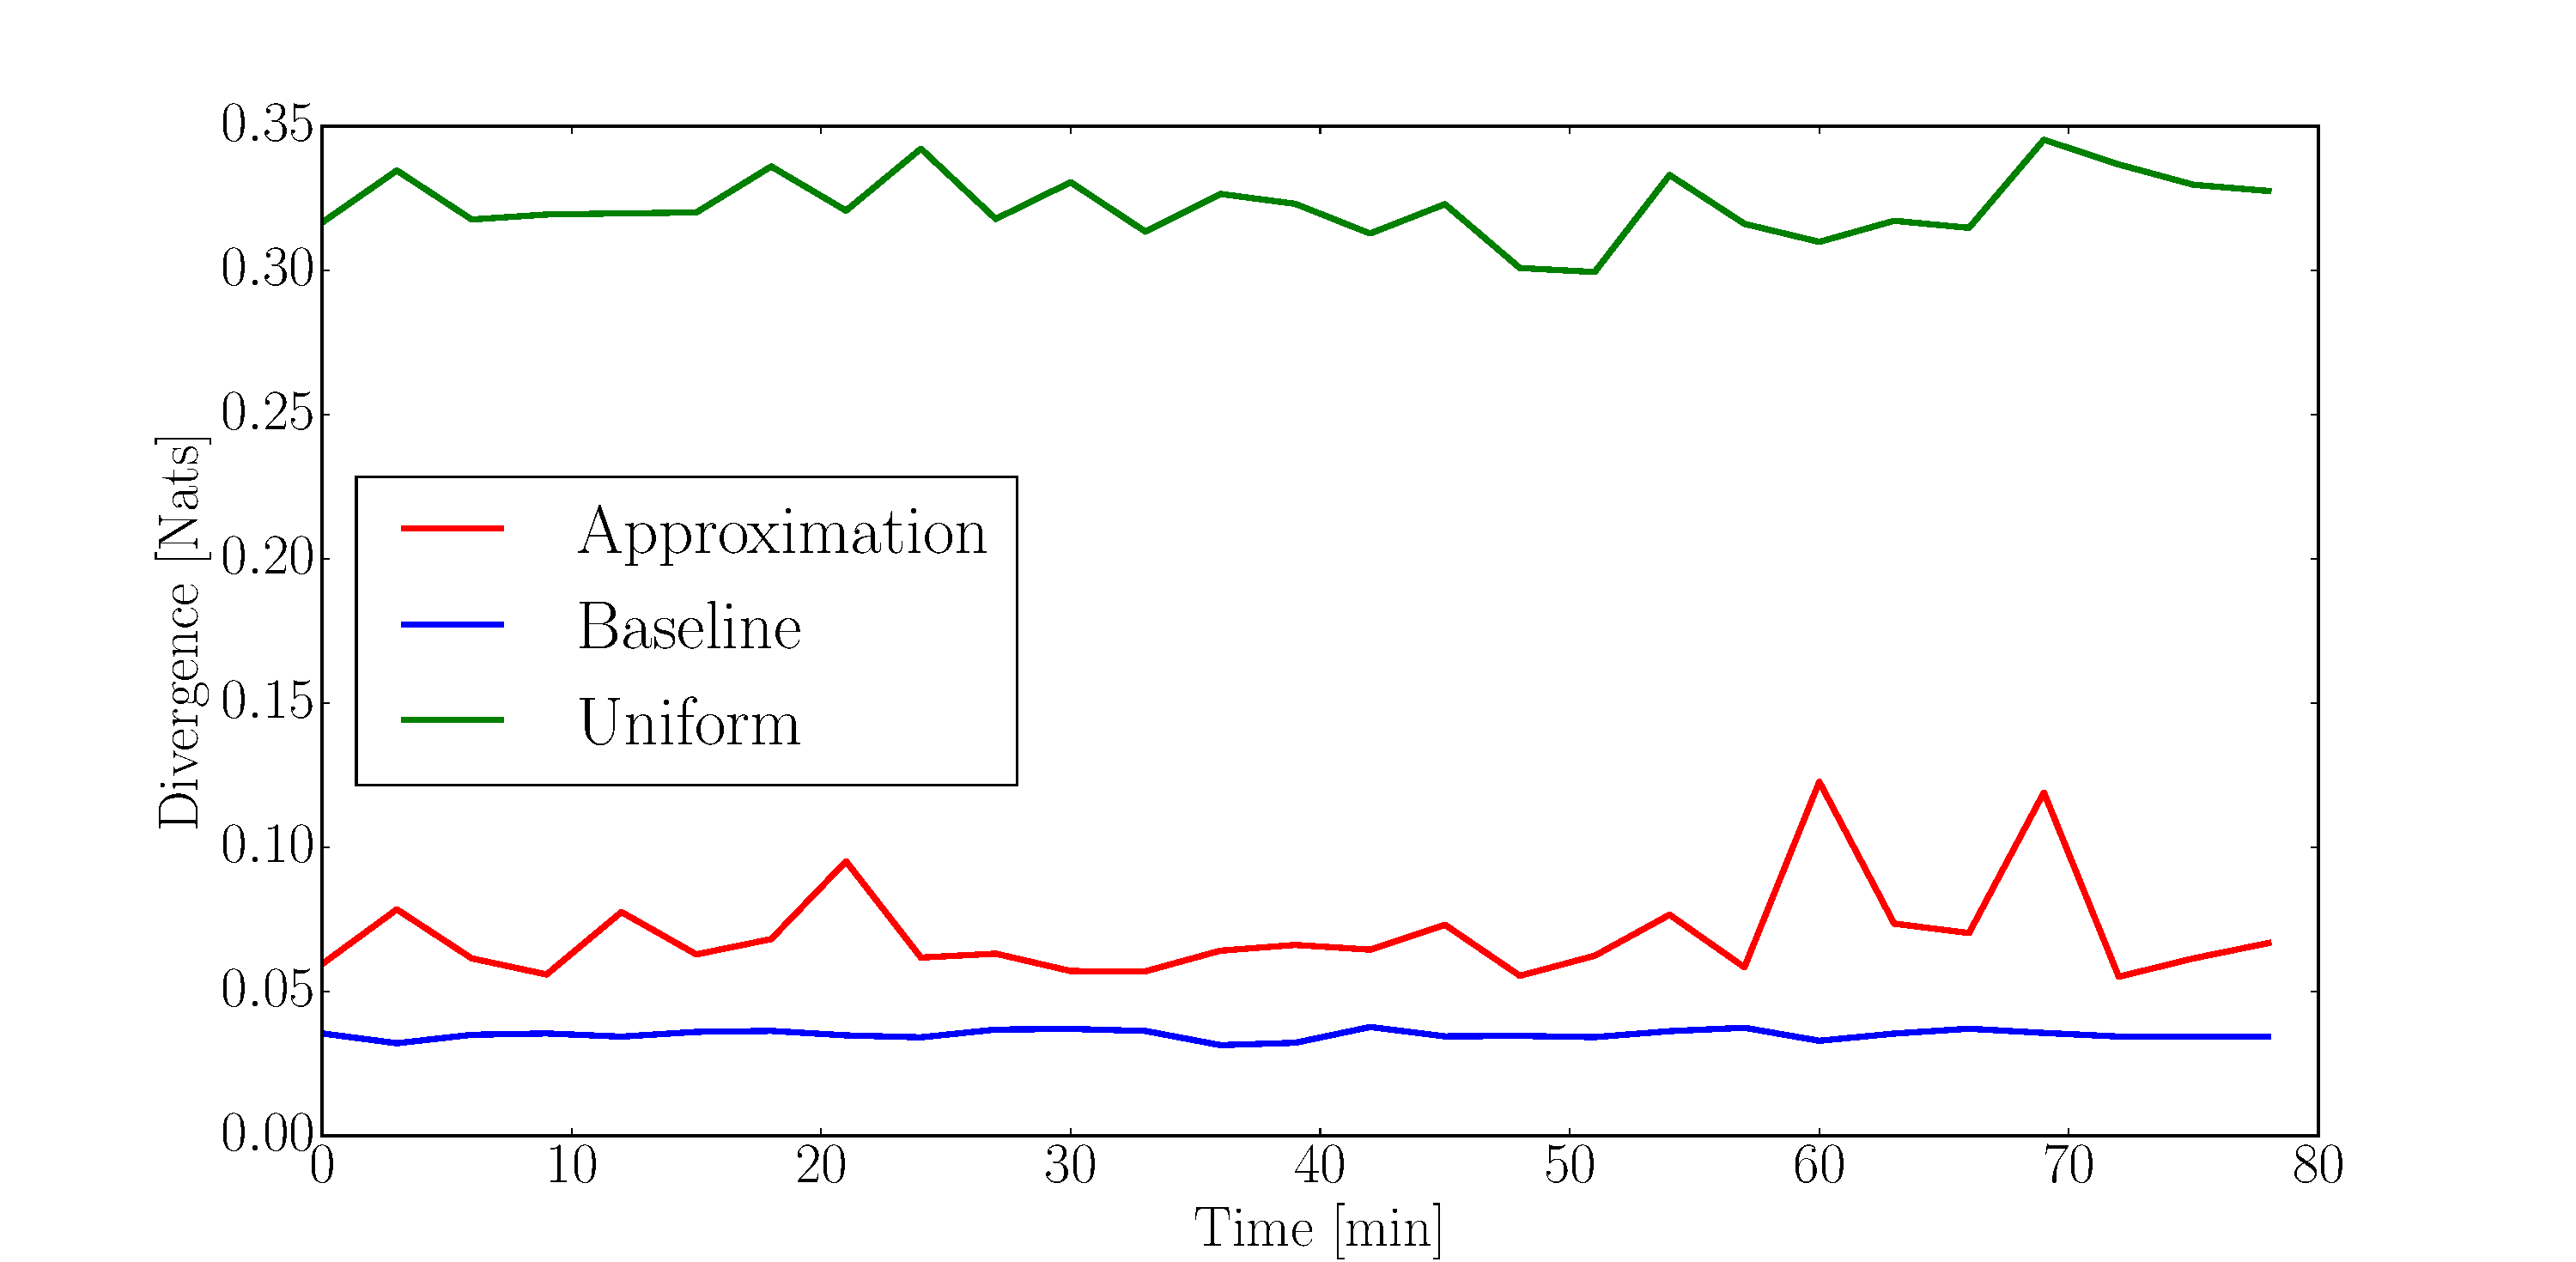
\includegraphics[scale=0.25]{lin_mod_kl.pdf}
\caption{Kullback-Leibler Divergence between the assumed Gaussian distribution and different sampled distributions using 5000 particles. The underlying model is linear. A log scale is used because the uniform curve differs by more than an order of magnitude from the other curves.}
\label{fig_lin_mod_kl}
\end{figure}
The approximation curve in Figure \ref{fig_lin_mod_kl} shows how much the samples diverge from the Gaussian distribution approximated using the samples. The baseline curve shows how much the Gaussian distribution diverges from samples of the same distribution. The uniform curve shows how much a Gaussian approximation of a Uniform distribution drawn in the interval $(\mu_i-\sigma_i, \mu_i-\sigma_i)$ (for each $i$ in the dimension of the underlying distribution) diverges; this serves to illustrate the divergence one would expect if attempting to model a distribution which is decidedly not normal. One would expect the baseline curve to tend to zero as the number of particles tends to infinity. Sampling error causes divergence from zero for the baseline curve. Thus we can use the baseline and uniform curves as a crude measure of normality.

In Figure \ref{fig_lin_mod_kl} we see that the approximation is relatively close to the baseline. Additionally it is far removed from the uniform curve. The average divergence for the baseline, approximation and uniform curve (in nats) is: $0.035$, $0.066$ and $34.57$ respectively. This implies that even though we are using a non-linear control technique the posterior state distributions are still approximately Gaussian. 


\subsection{Nonlinear System}
In this section we consider the problem of controlling the full non-linear system with a linear model linearised around the unsteady operating point. The control goal is the same as before; the only difference between this section and Section \ref{sec_lin_sys_cont} is that the underlying plant is non-linear.

The linear control model and noise parameters are the same as (\ref{eq_linmod_params}). The control tuning parameters are the same as (\ref{eq_mpc_tuning}).

As before we first investigate the LQG controller. The control problem is the same as (\ref{eq_lqg_linmod}) but this time the underlying system is non-linear. Figure \ref{fig_nonlin_lqg} shows the unconstrained reference tracking results.
\begin{figure}[H] 
\centering
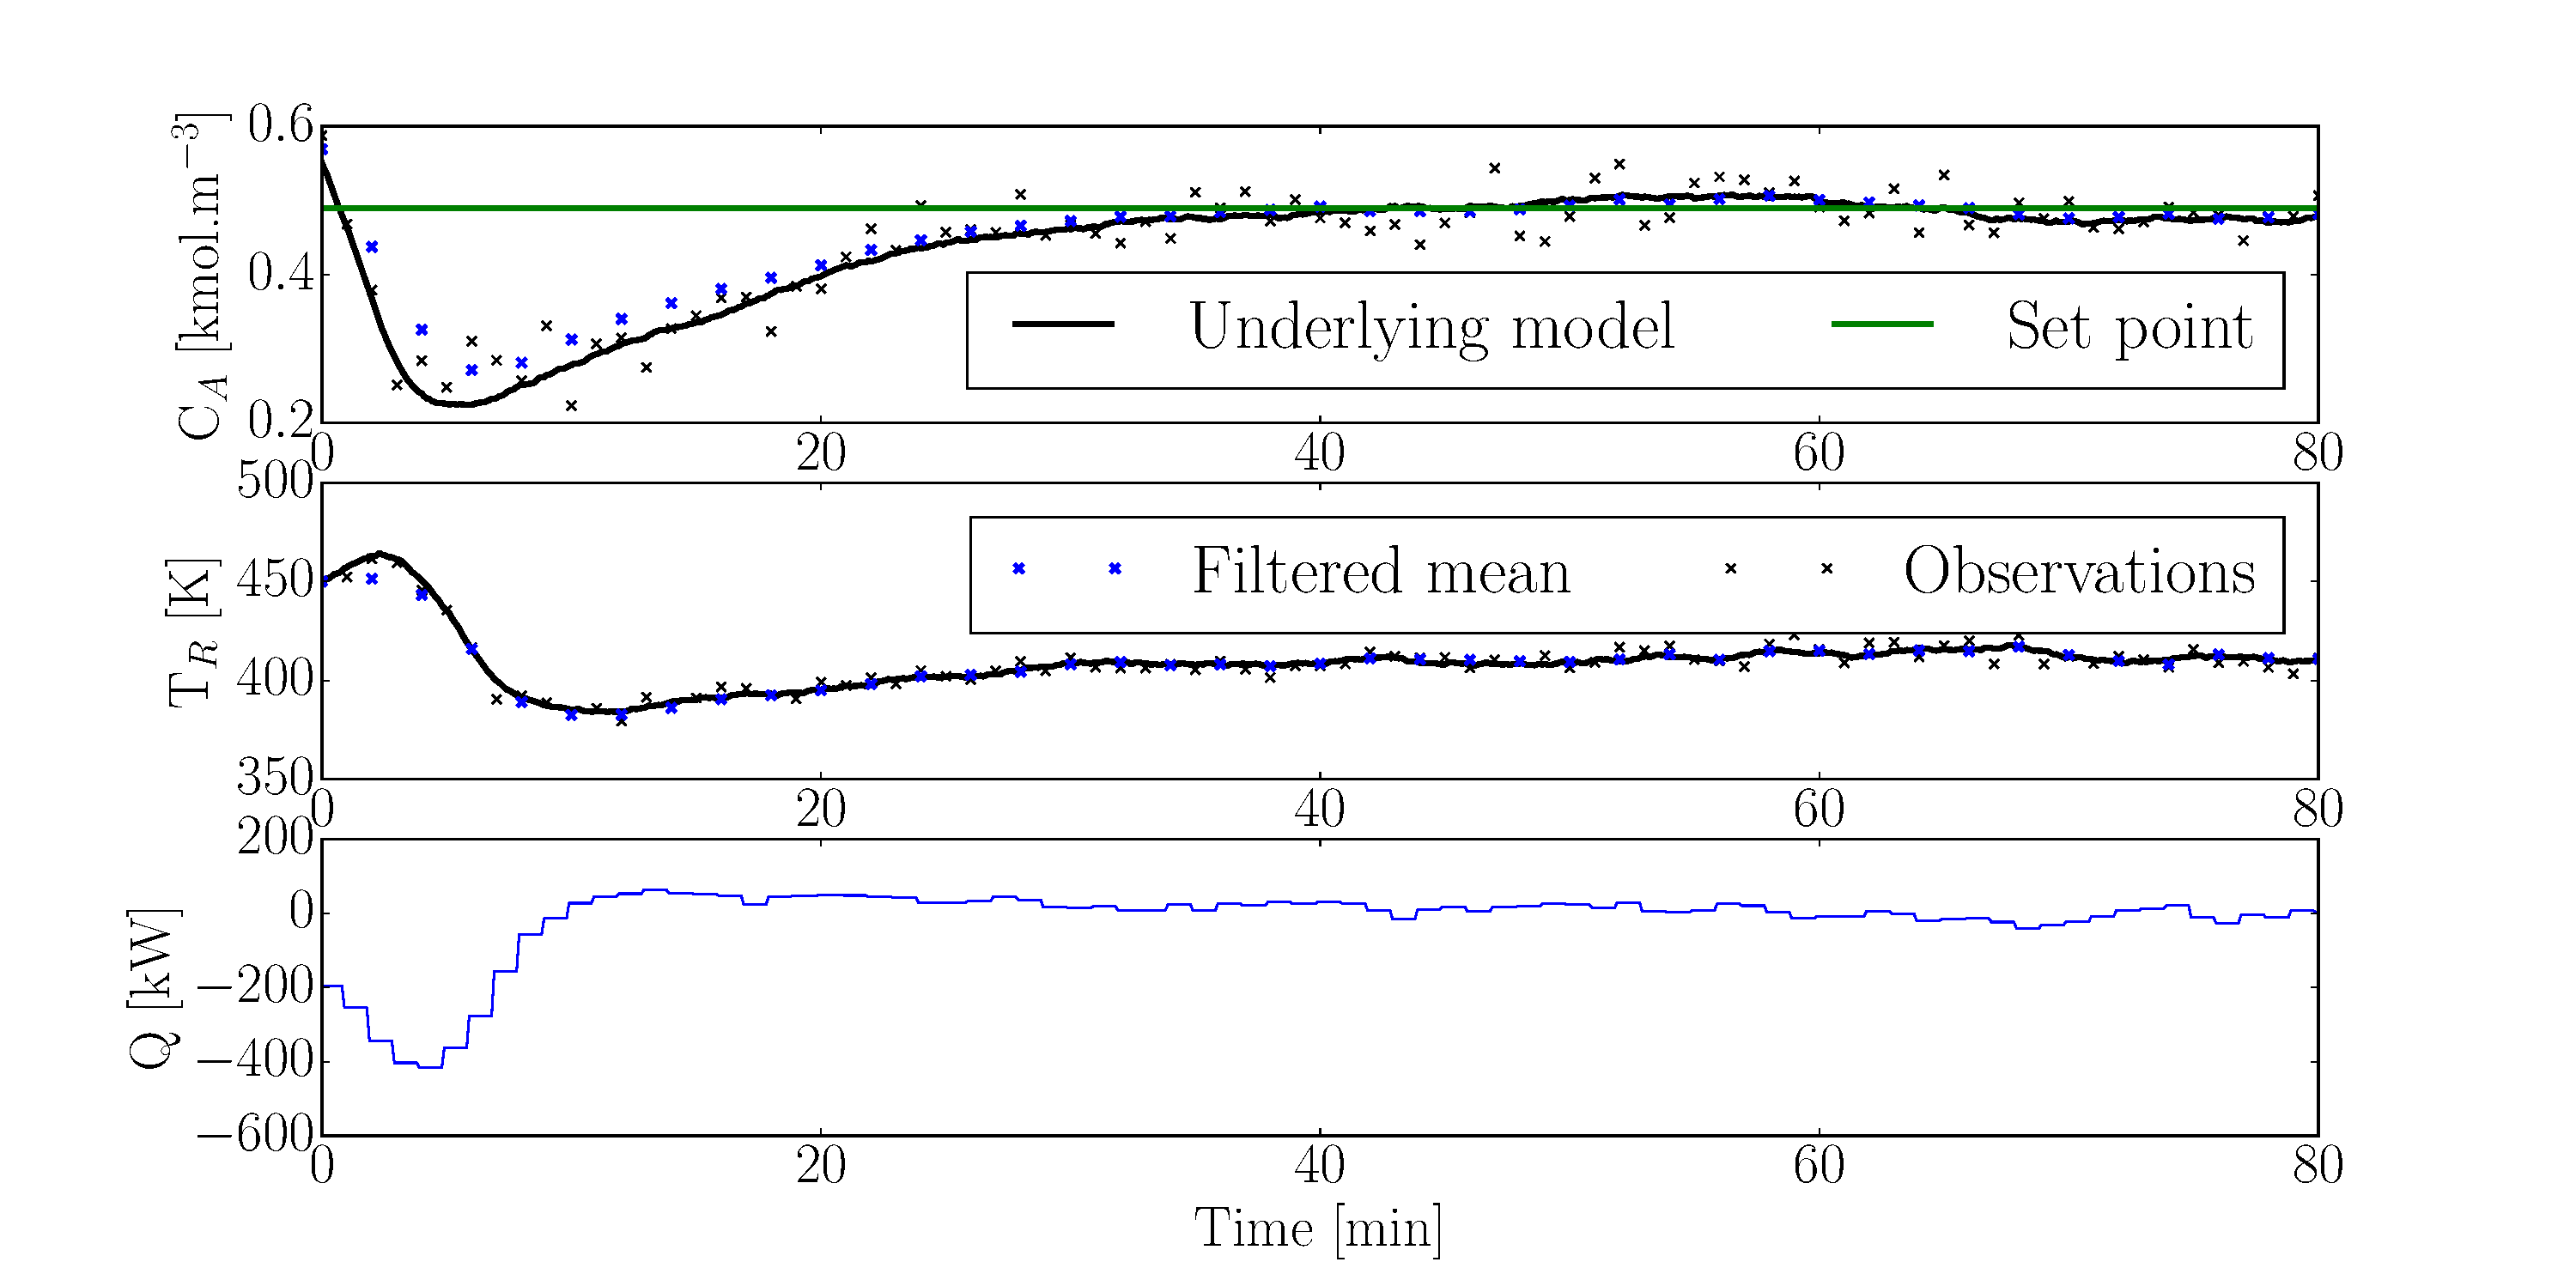
\includegraphics[scale=0.25]{nonlin_mod_lqg.pdf}
\caption{LQG regulator tracking with initial condition (0.55, 450) and measuring both states.}
\label{fig_nonlin_lqg}
\end{figure}
The average energy usage and concentration error was 302 kJ/min and 10.94\% respectively over the 80 min simulation time. Comparing Figures \ref{fig_lin_mod_lqg} and \ref{fig_nonlin_lqg} we see that the maximum absolute input energy is much greater with the non-linear underlying dynamics. This is not unexpected because the controller in both cases is linear: one expects that the plant-model mismatch to have a detrimental effect on control.

In the previous section we had a linear underlying model and linear control. Figure \ref{fig_lin_mod_kl} also demonstrated that the posterior state distributions were approximately Gaussian. Thus there was no reason to use non-linear inference algorithms like the Particle Filter introduced in Section \ref{sec_inf_nonlin_mods}. However, in this section we are using a non-linear underlying model and it might be advantageous to use a more sophisticated inference tool. We investigate using both a Kalman Filter and a Particle Filter for inference. In the setting of the Particle Filter we approximate the samples as Gaussian and use that for control.

As before we first investigate the deterministic MPC. The control problem is shown in (\ref{eq_mpc_constrained_det2}). Note that the constraints are different due to the expected extra difficulty introduced by the non-linear underlying model. 
\begin{equation}
\begin{aligned}
&\underset{\mathbf{u}}{\text{min }} \frac{1}{2}\sum_{k=0}^{N-1} \left( \mu_k^TQ\mu_k + u_k^TRu_k \right) + \frac{1}{2}\mu_N^TP_f\mu_N \\
& \text{subject to } \mu_{t+1}=A\mu_t + Bu_t \\
&\text{and } \begin{pmatrix}
10 \\ 1
\end{pmatrix}^T \mu_t + 400 \geq 0 ~\forall ~t=1,...,N\\
& \text{and } |u_t| \leq 20000 ~\forall ~t=0,...,N-1\\
\end{aligned}
\label{eq_mpc_constrained_det2}
\end{equation}
In Figure \ref{fig_nonlin_mod_kf_mean_track} we see that the deterministic MPC using the Kalman Filter for state inference does converge to the set point. The ability to naturally constrain the system is again highlighted in the input: as opposed to the -25 000 kJ/min required by the LQG controller the MPC manages to control the system while never requiring more than $|20000|$ kJ/min. 
\begin{figure}[H] 
\centering
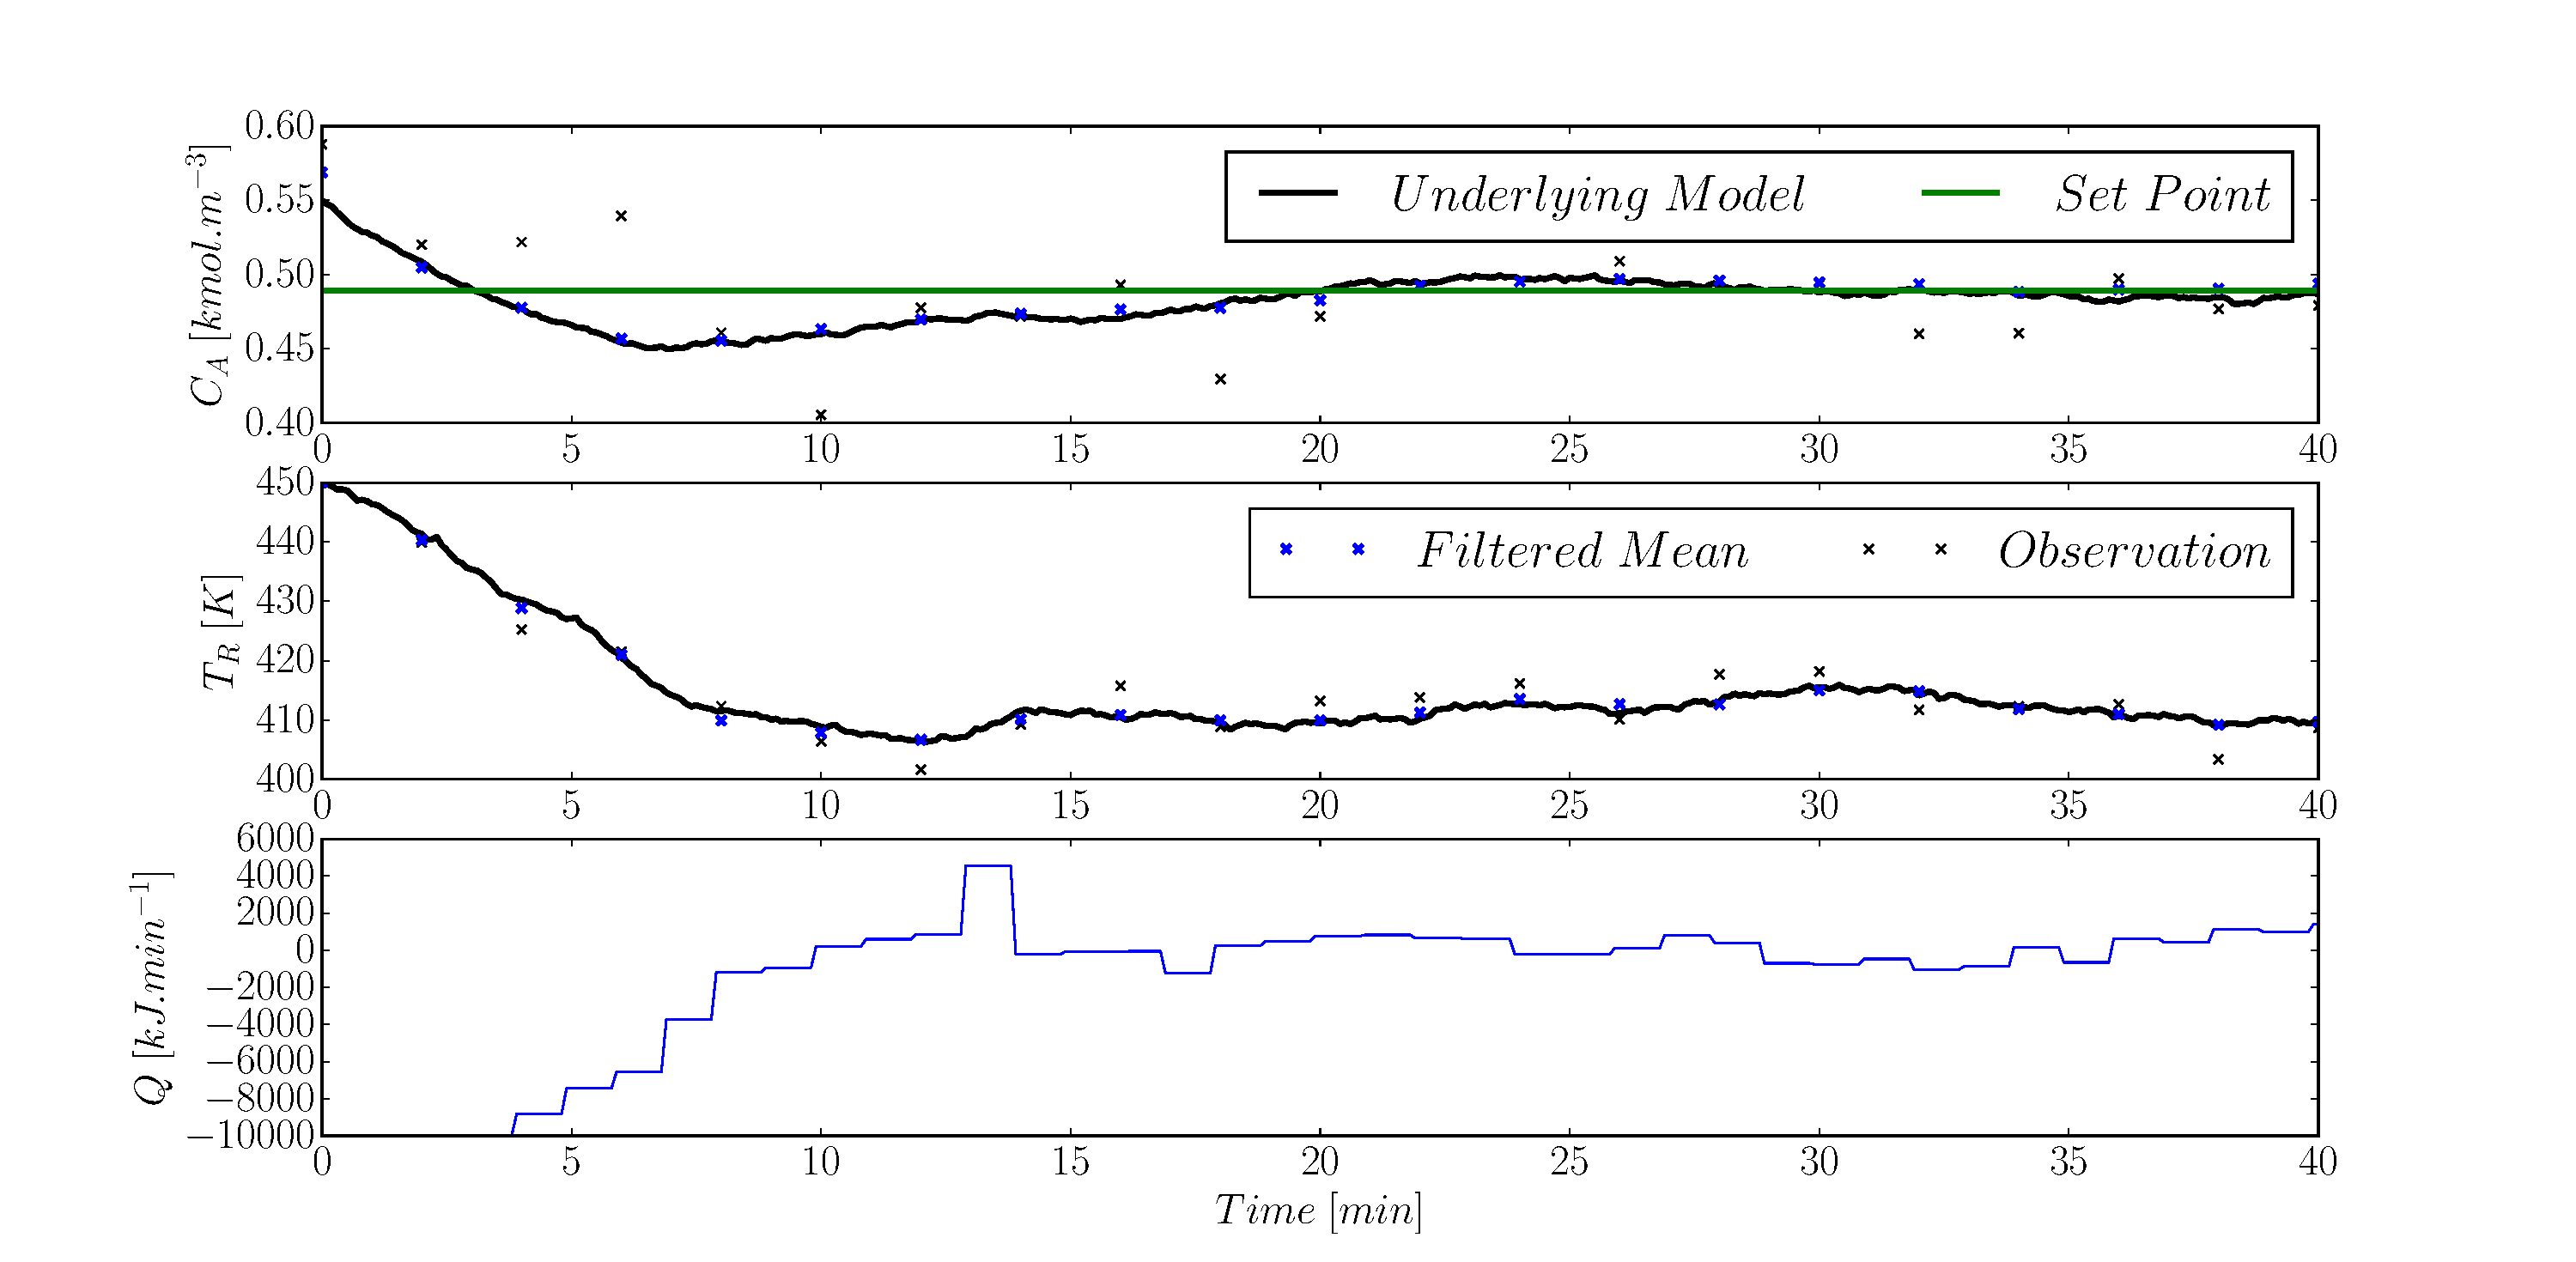
\includegraphics[scale=0.25]{lin_mod_kf_mean_track.pdf}
\caption{Deterministic constrained MPC reference tracking with initial condition $(0.55, 450)$ and measuring both states. The Kalman Filter is used for inference.}
\label{fig_nonlin_mod_kf_mean_track}
\end{figure} 
In Figure \ref{fig_nonlin_mod_kf_mean_ss} we see that the state constraint is violated just like Figure \ref{fig_lin_mod_kf_mean_ss}. We also see a somewhat unrealistic jagged state trajectory but this is just a numerical artefact. The average energy input and concentration error over the simulation run is 413 kJ/min and 14.53\% respectively. Once again the added constraints explain why the performance is degraded when compared to the LQG controller.
\begin{figure}[H] 
\centering
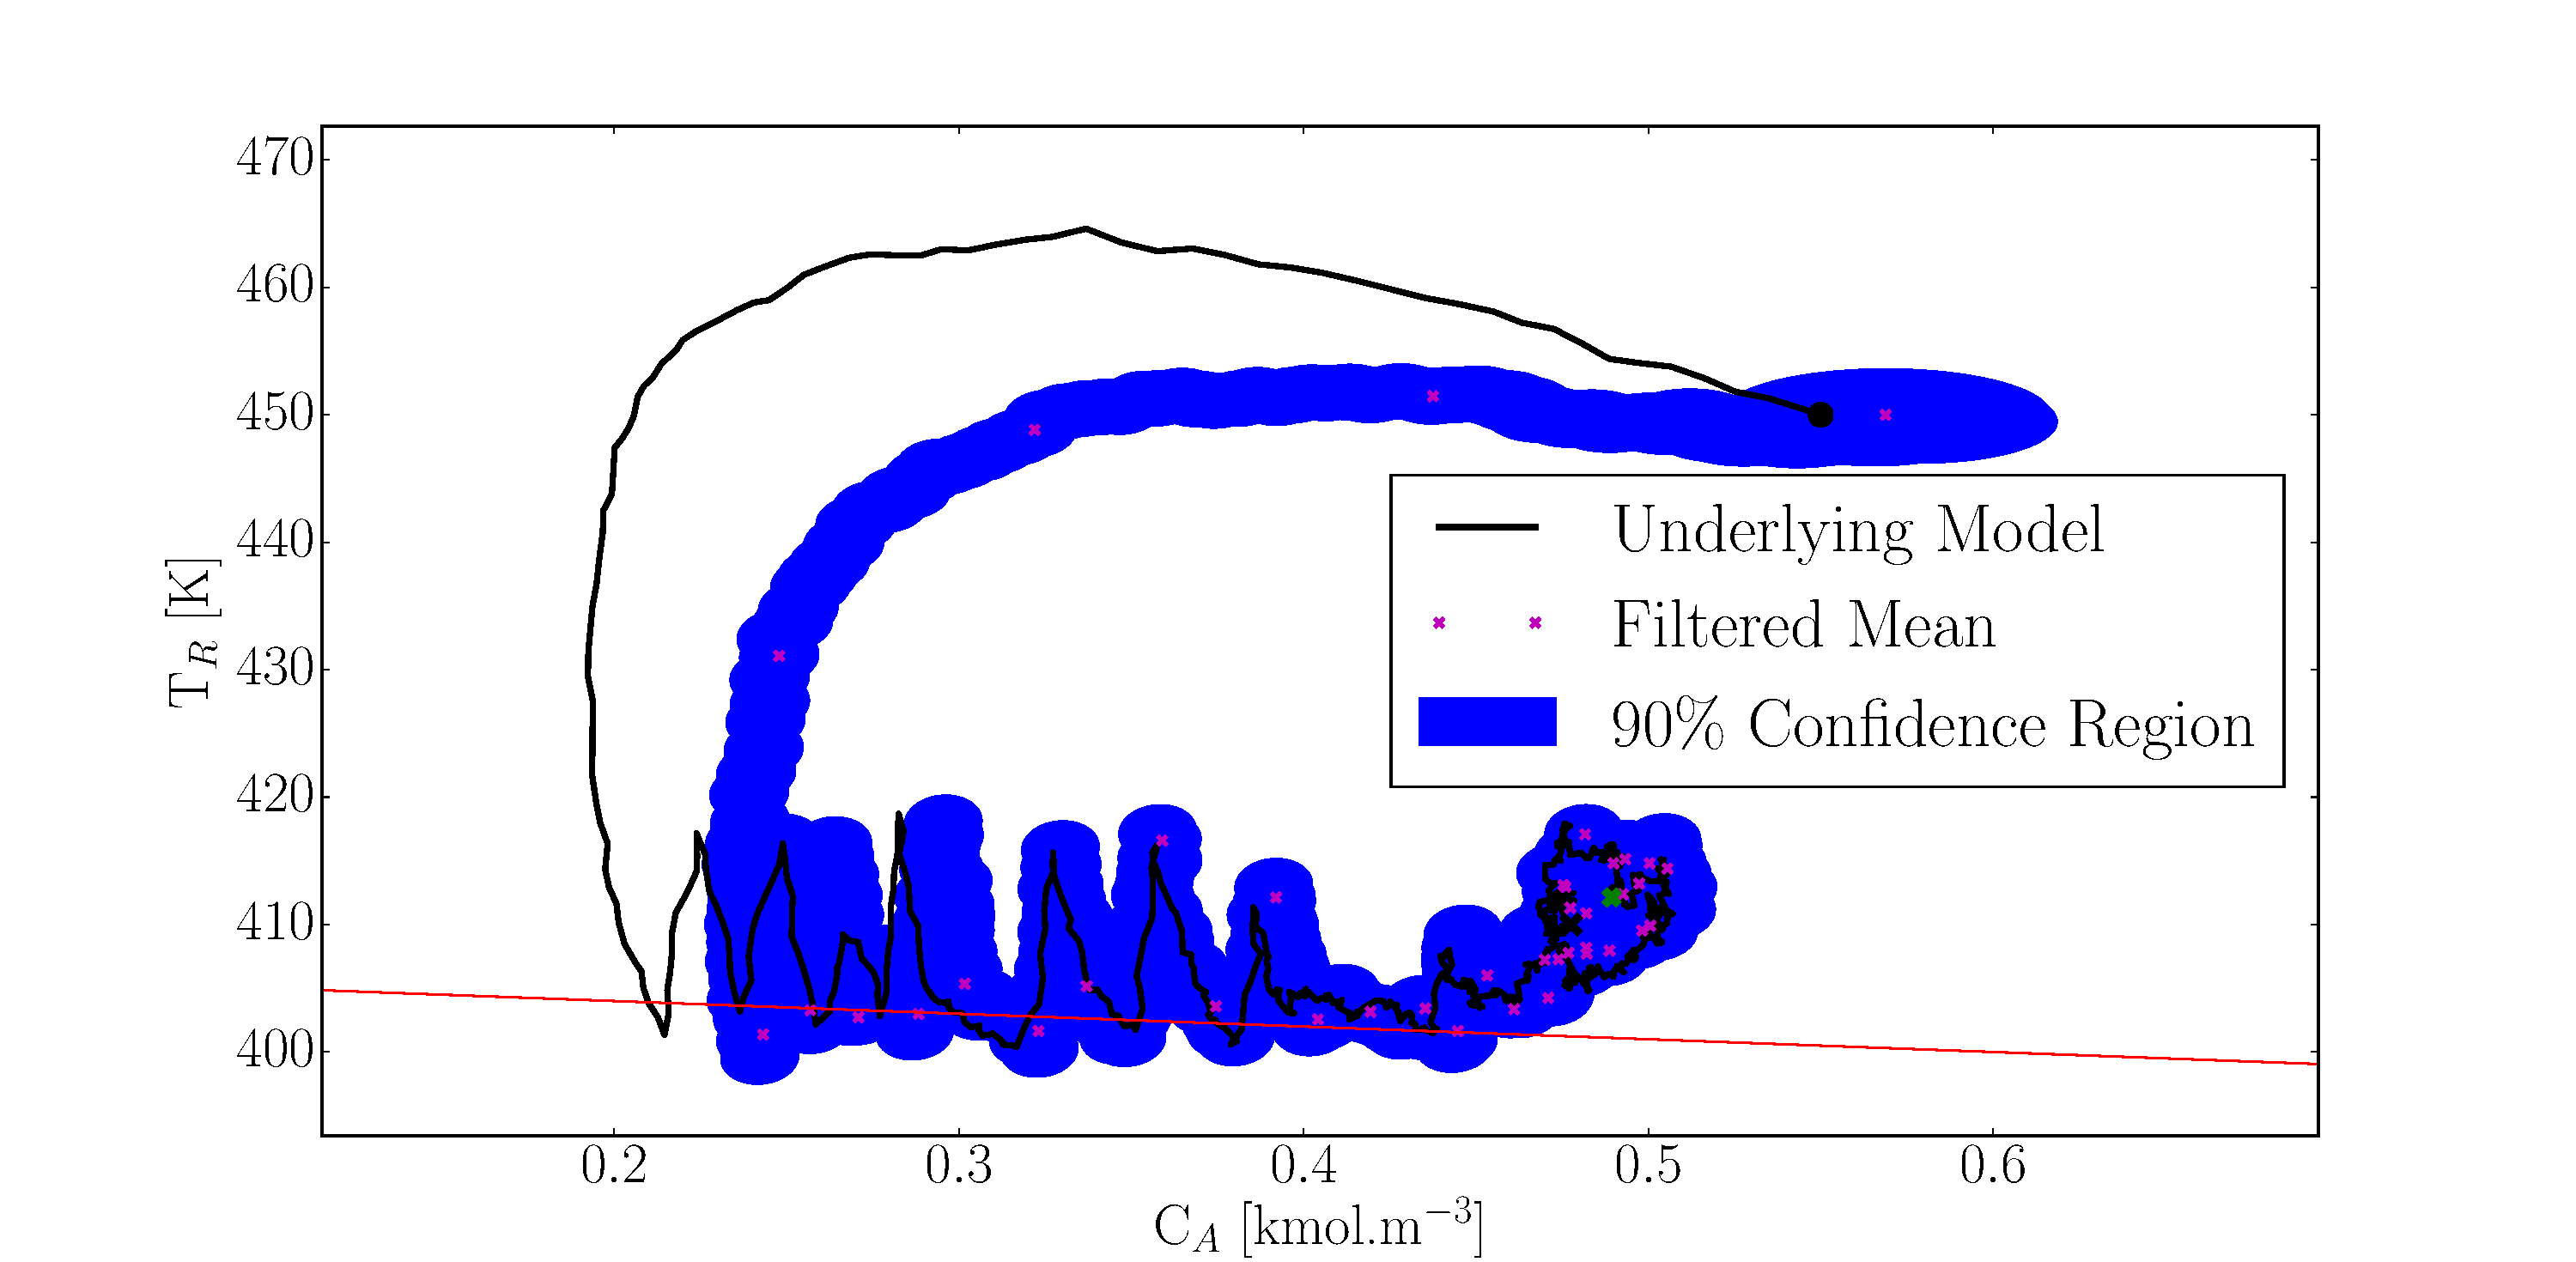
\includegraphics[scale=0.25]{nonlin_mod_kf_mean_ss.pdf}
\caption{Deterministic constrained MPC state space trajectory with initial condition $(0.55, 450)$ and measuring both states. The Kalman Filter is used for inference.}
\label{fig_nonlin_mod_kf_mean_ss}
\end{figure}
Since we are not using a stochastic MPC the state constraint violation is not surprising in Figure \ref{fig_nonlin_mod_kf_mean_ss}. However, a more significant issue is the inability of the Kalman Filter to accurately track the states throughout the simulation (the underlying system briefly diverges from the state estimates). This can be significantly problematic if a constraint existed in the left hand side of the state space: the controller wouldn't know that it was violating the constraint because the state estimate is poor. This behaviour is caused by the linear model used by the Kalman Filter. The state trajectory moves away from the region close to the linearisation point and thus, as explained in Section \ref{sec_inf_lin_mods}, the state estimate becomes poor.

We can remedy this situation by using a more sophisticated inference algorithm. In Figure \ref{fig_nonlin_mod_pf_mean_track} we see the deterministic MPC using a Particle Filter with 200 particles for inference. 
\begin{figure}[H] 
\centering
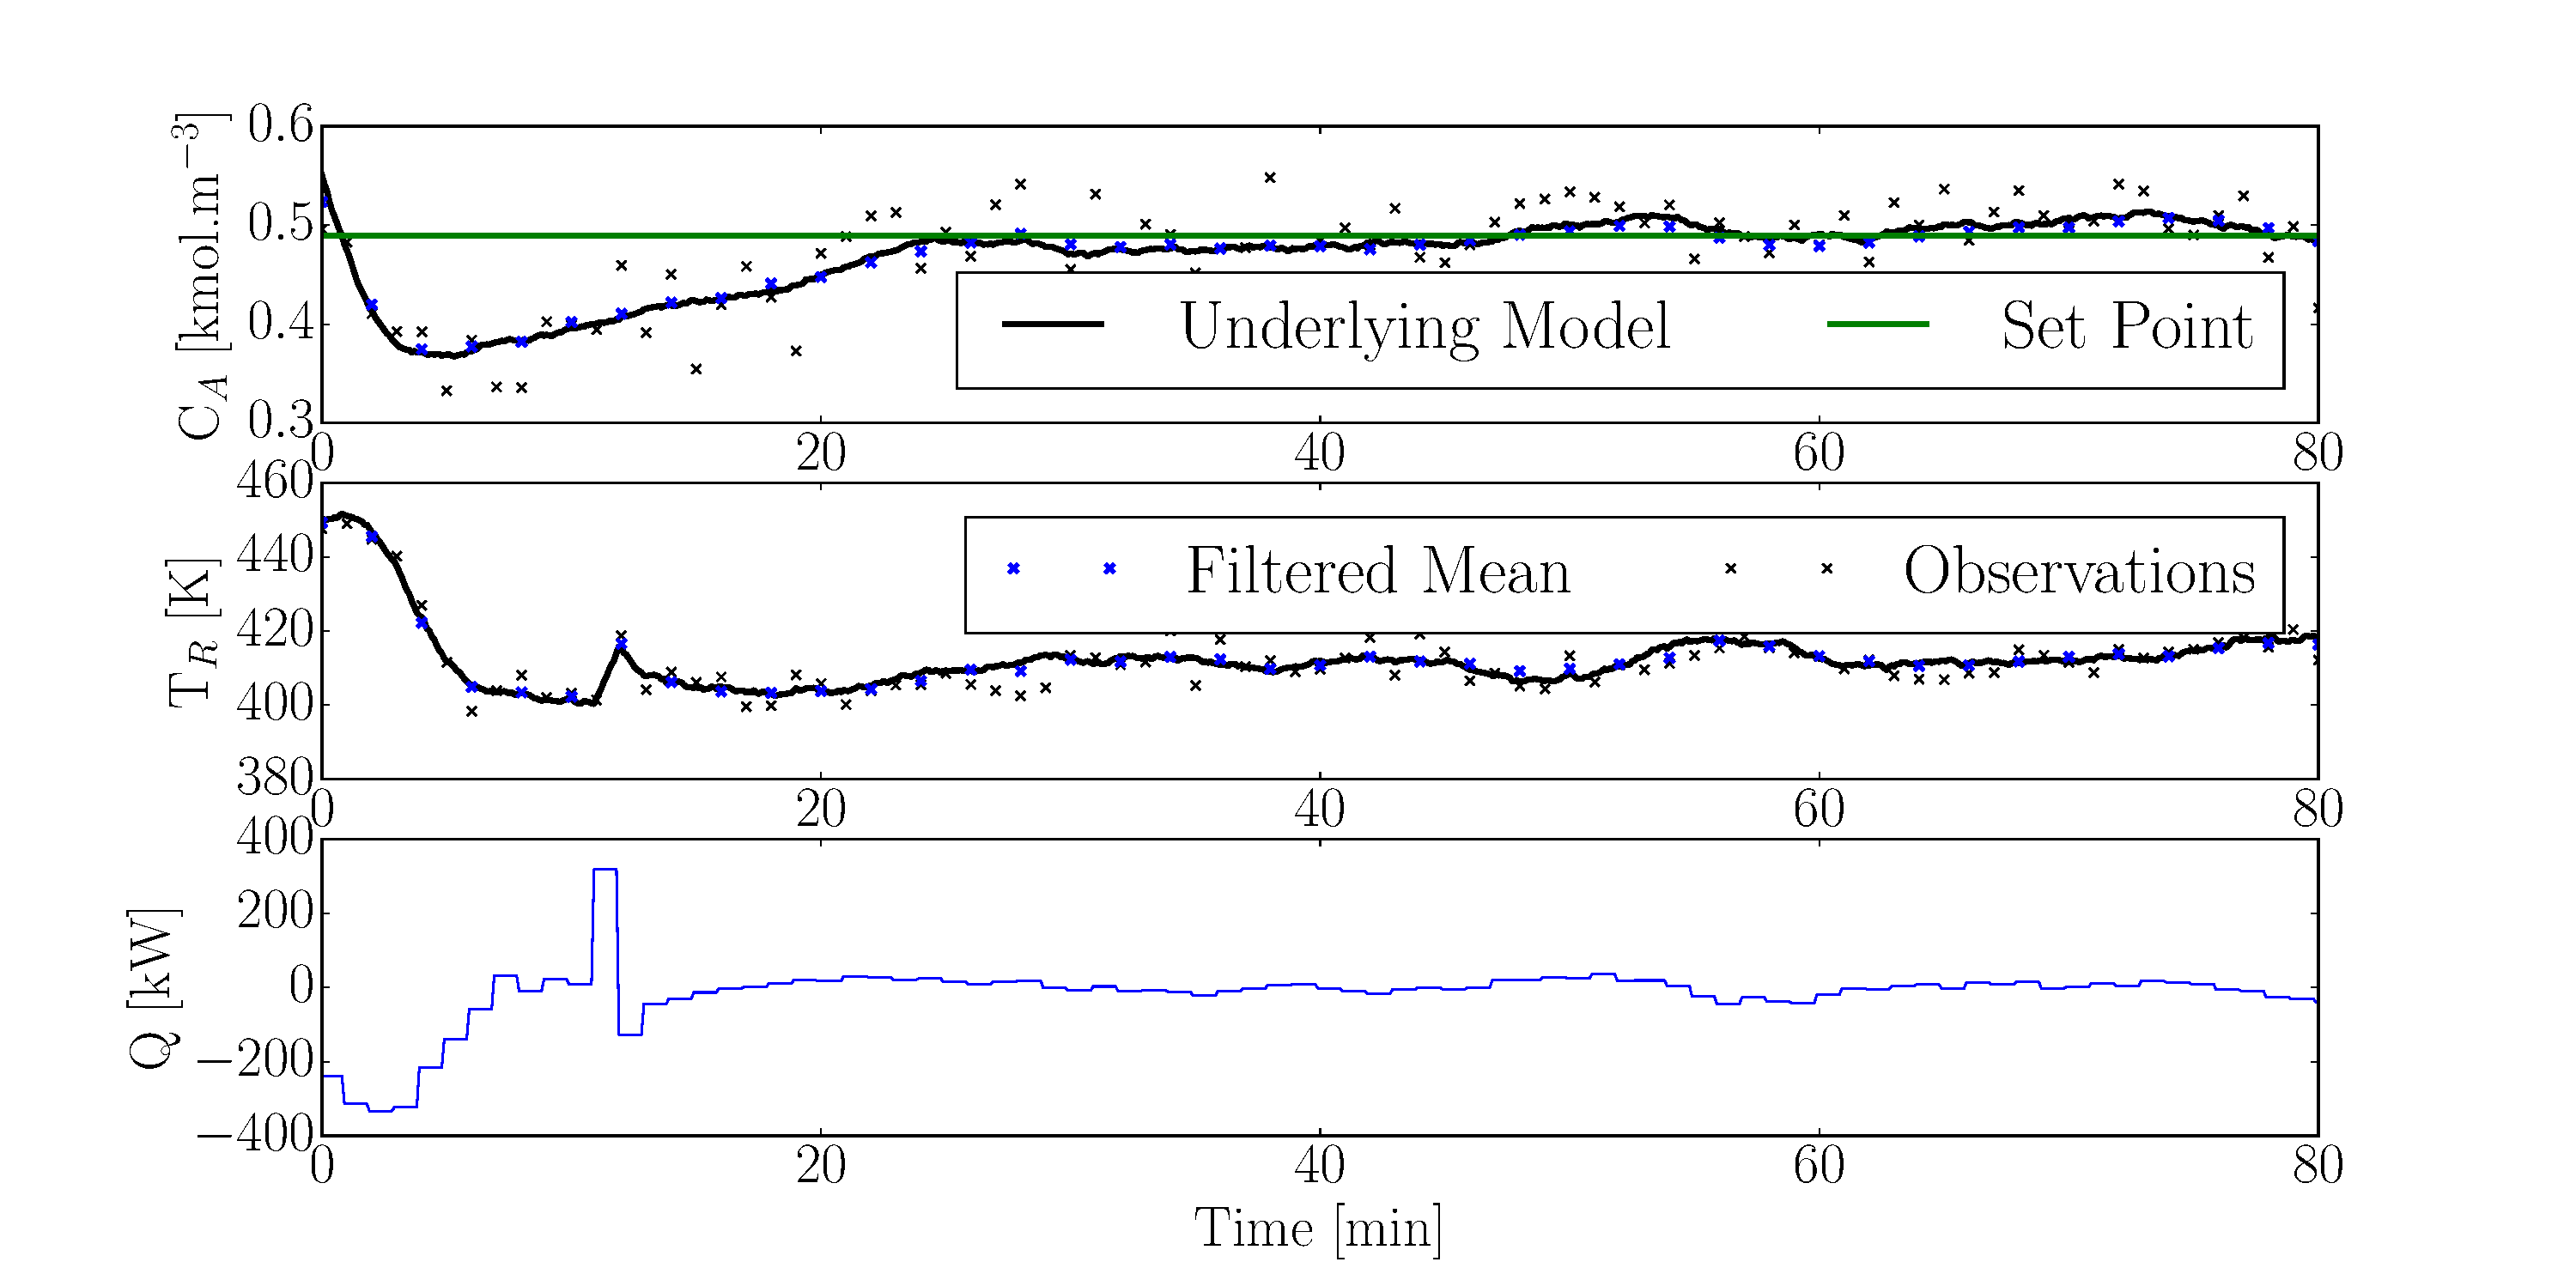
\includegraphics[scale=0.25]{nonlin_mod_pf_mean_track.pdf}
\caption{Deterministic constrained MPC reference tracking with initial condition $(0.55, 450)$ and measuring both states. A Particle Filter with 200 particles is used for inference.}
\label{fig_nonlin_mod_pf_mean_track}
\end{figure} 
The average energy input and concentration error is 218 kJ/min and 4.80\% respectively. This is a vast improvement over the same controller where the Kalman Filter was used for inference. The benefit of accurate state estimation is apparent here and also in Figure \ref{fig_nonlin_mod_pf_mean_ss}.
\begin{figure}[H] 
\centering
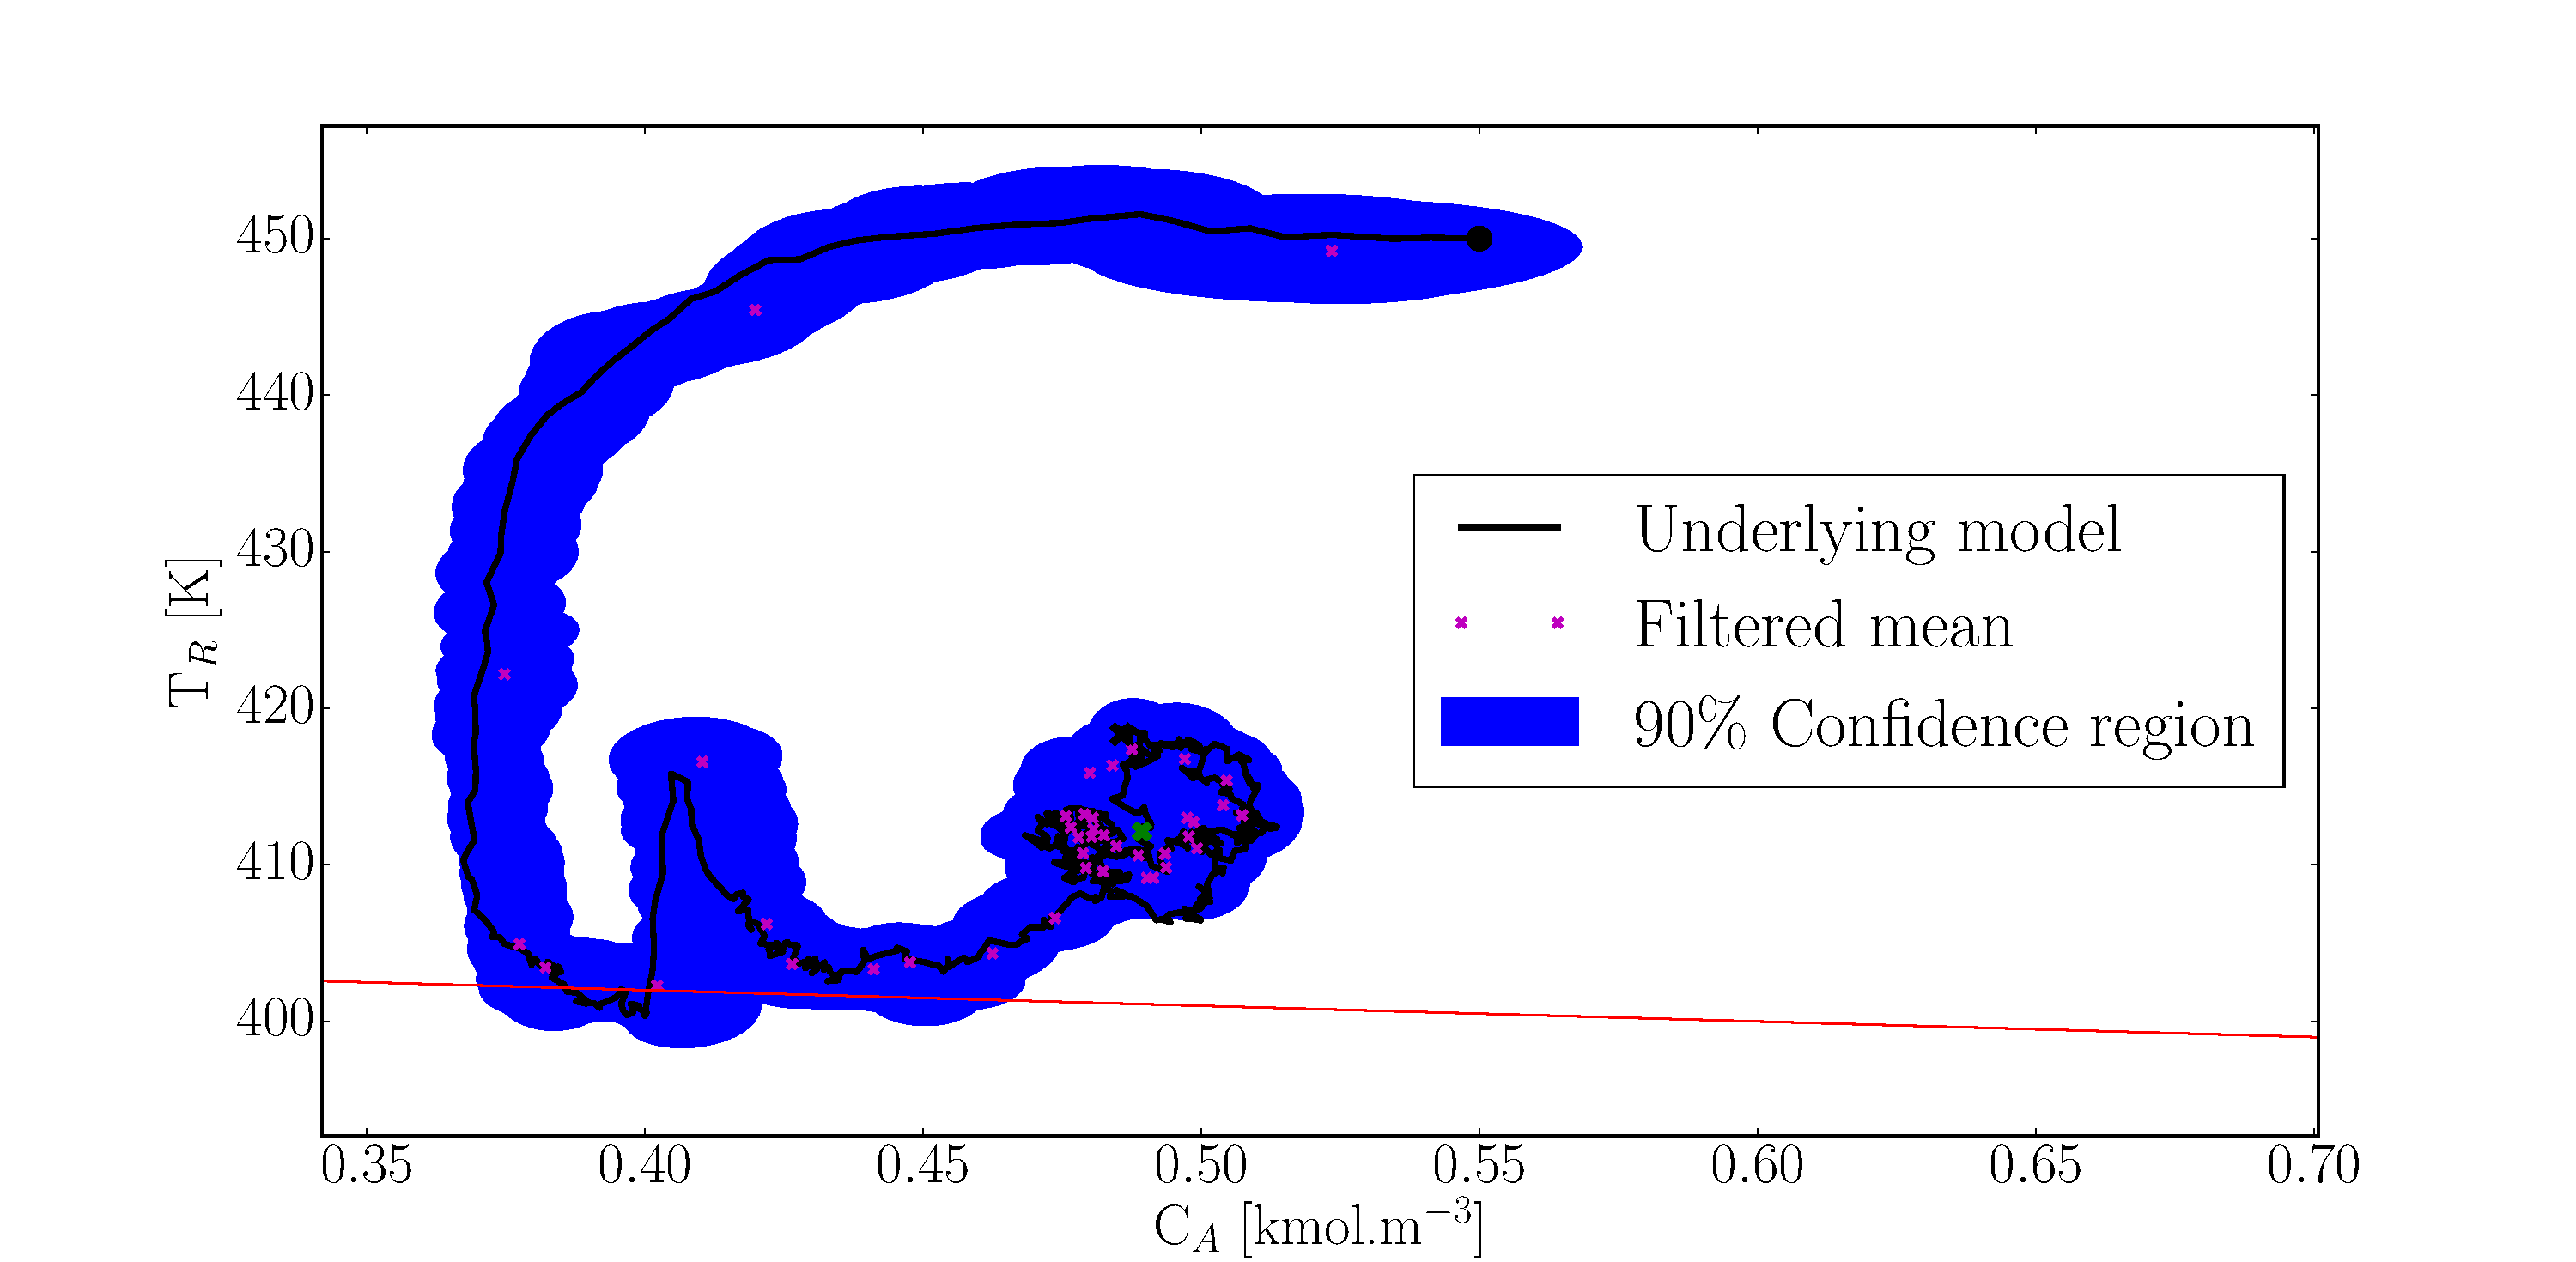
\includegraphics[scale=0.25]{nonlin_mod_pf_mean_ss.pdf}
\caption{Deterministic constrained MPC state space trajectory with initial condition $(0.55, 450)$ and measuring both states. A Particle Filter with 200 particles is used for inference.}
\label{fig_nonlin_mod_pf_mean_ss}
\end{figure}
In Figure \ref{fig_nonlin_mod_kf_mean_ss} we saw significant estimation deviation from the true underlying state, while in Figure \ref{fig_nonlin_mod_pf_mean_ss} the deviation is negligible. We still have that the state constraint is violated but this is due to the stochastic nature of the underlying system. It is clear that the Particle Filter MPC combination is superior to the Kalman Filter MPC combination in this case. However, the benefit of using the Particle Filter should be weighed against the cost of the algorithm especially in higher dimensions where it is known that the Particle Filter does not perform well (recall the discussion following Figure \ref{fig_pf_kf_phase2}).

Now we introduce the stochastically constrained MPC in (\ref{eq_mpc_nonlin_mod_cons}). Note that the constraints are different than (\ref{eq_mpc_linmod_kf_cons}) for the same reason as (\ref{eq_mpc_constrained_det2}). We have $d^T = (10, 1)$ and $e=400$ as before. By consulting a Chi-Squared Distribution table we set $k^2 = 4.6052$ which corresponds to the chance constraint $\text{Pr}(d^Tx_t + e \geq 0) \geq 90\% ~\forall ~t=1,...,N$ exactly as in the previous section.
\begin{equation}
\begin{aligned}
&\underset{\mathbf{u}}{\text{min }} \frac{1}{2}\sum_{k=0}^{N-1} \left( \mu_k^TQ\mu_k + u_k^TRu_k \right) + \frac{1}{2}\mu_N^TP_f\mu_N + \frac{1}{2}\sum_{k=0}^N \text{tr}(Q\Sigma_k) \\
& \text{subject to } \mu_{t+1}=A\mu_t + Bu_t \\
& \text{and } \Sigma_{t+1} = W+A\Sigma_t A^T \\
& \text{and } d^T\mu_t + e \geq k\sqrt{d^T \Sigma_t d} ~\forall ~t=1,...,N\\
& \text{and } |u_t| \leq 20000 ~\forall ~t=0,...,N-1\\
\end{aligned}
\label{eq_mpc_nonlin_mod_cons}
\end{equation}
As with the deterministic case we first investigate the system where a Kalman Filter is used for inference. Figure \ref{fig_nonlin_mod_kf_var90_track} illustrates that the stochastically constrained system does indeed converge to the set point. The average energy input and concentration error is 384 kJ/min and 12.33\%. The average energy usage and average concentration error is reduced compared to the deterministic system. 
\begin{figure}[H] 
\centering
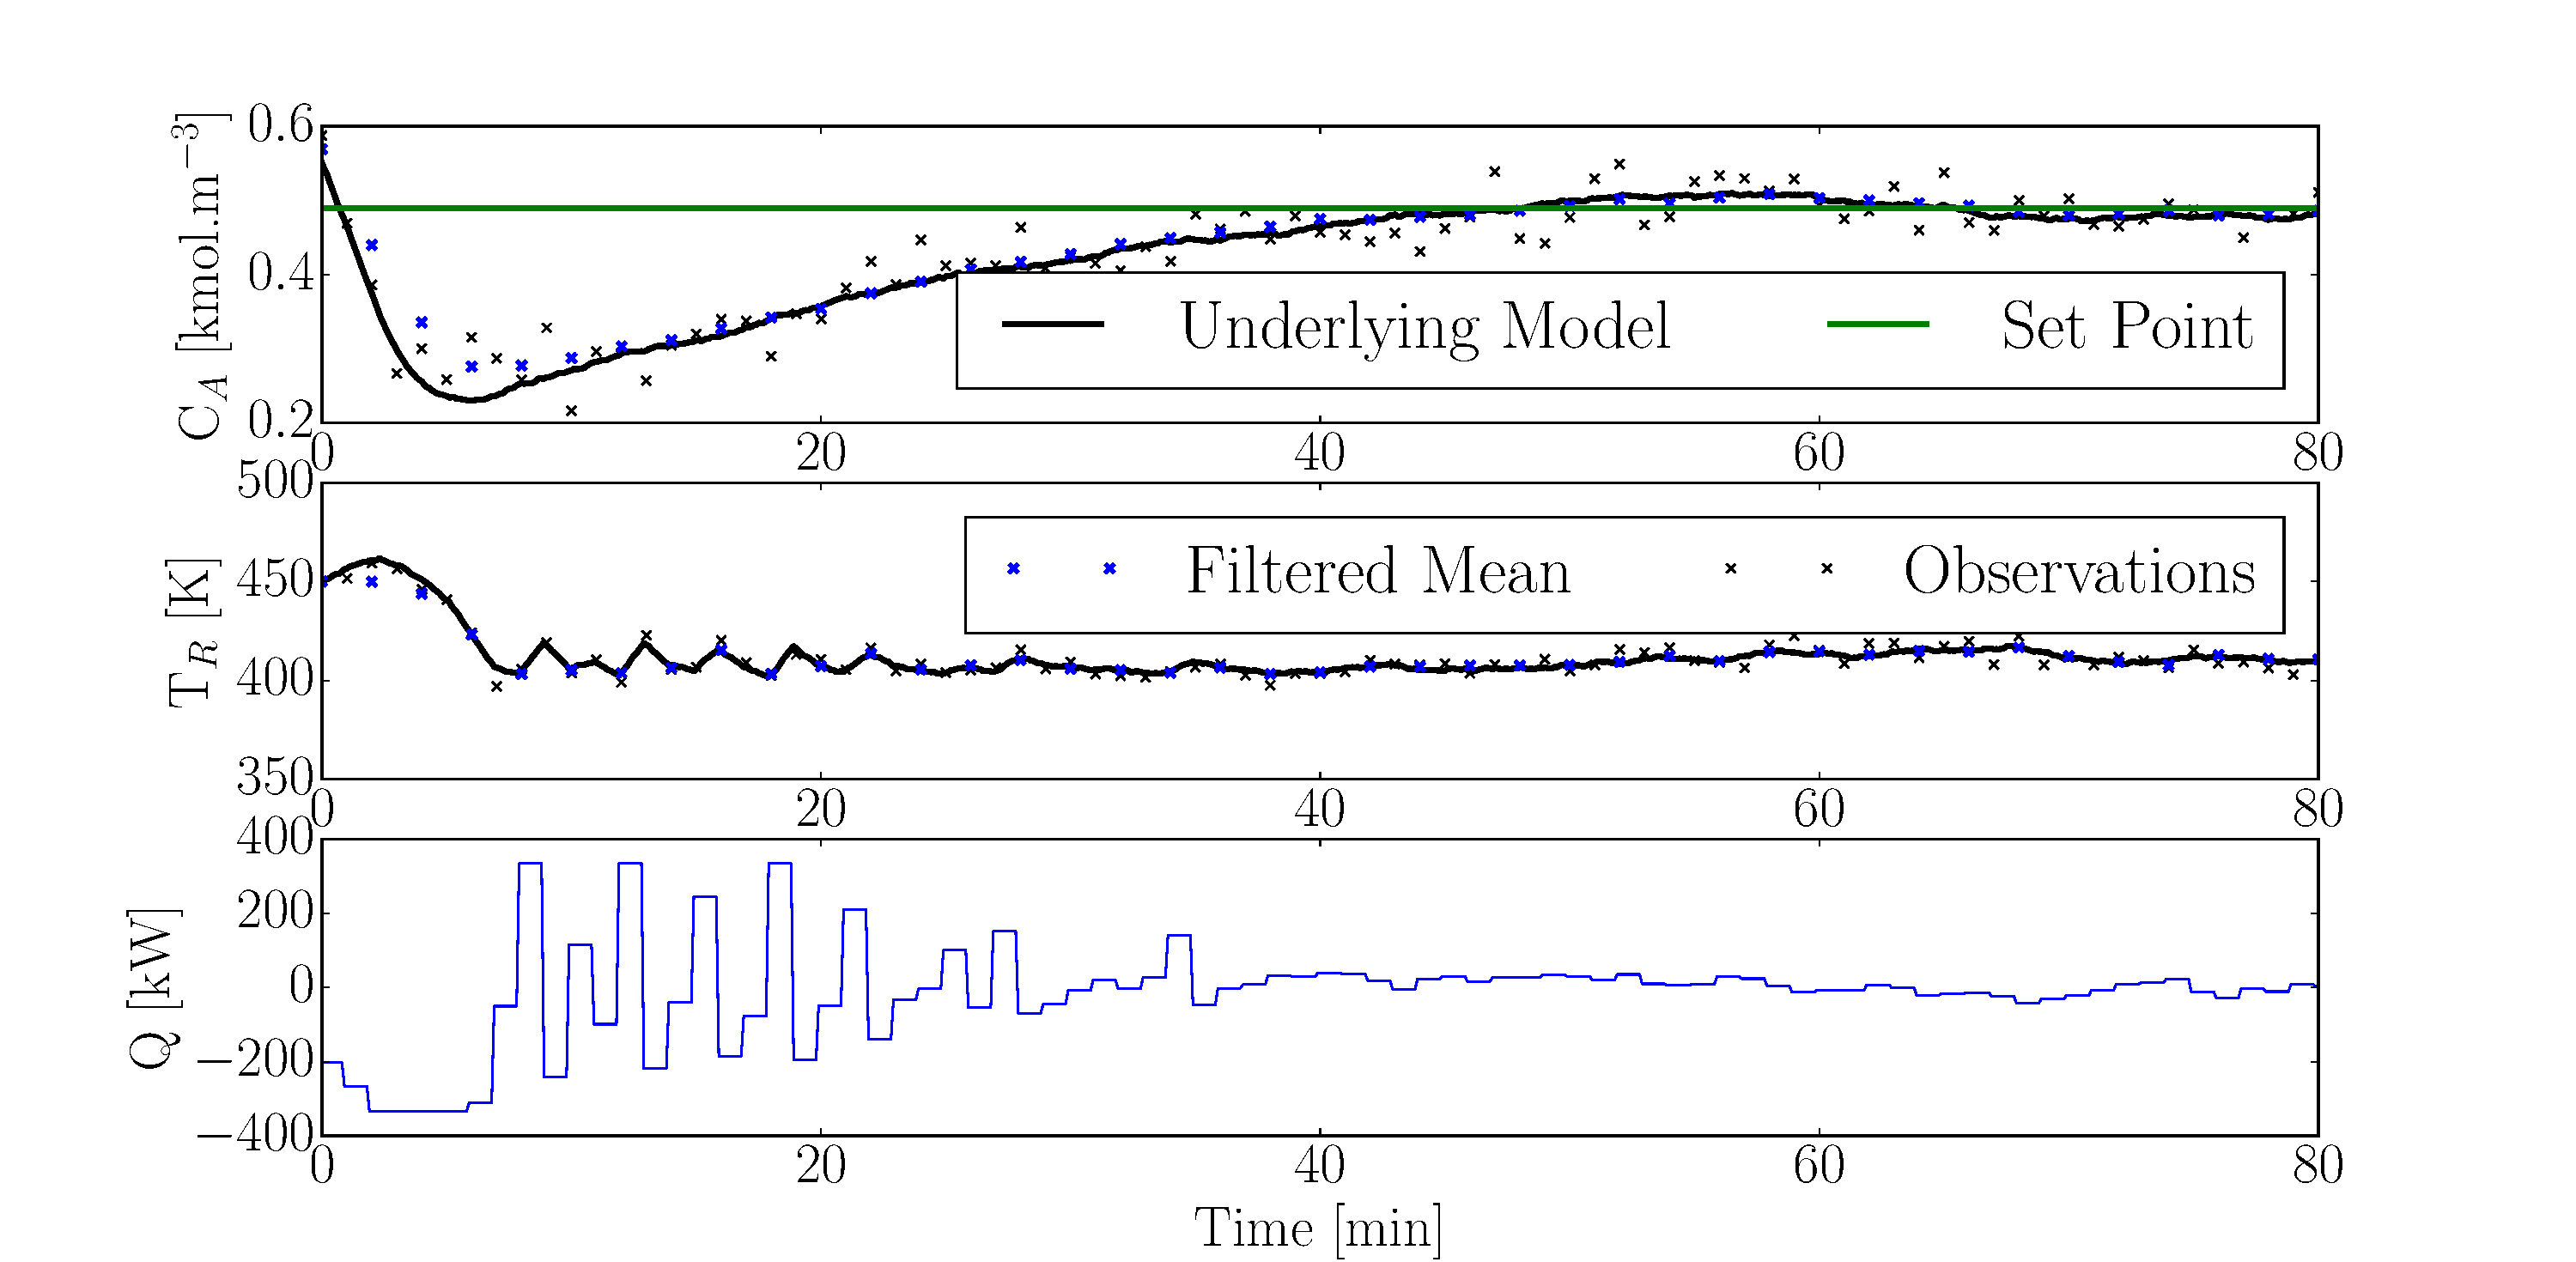
\includegraphics[scale=0.25]{nonlin_mod_kf_var90_track.pdf}
\caption{Stochastic constrained MPC tracking with initial condition $(0.55, 450)$ and measuring both states. A Kalman Filter is used for inference and the chance constraint is set at 90\%.}
\label{fig_nonlin_mod_kf_var90_track}
\end{figure}
Again the benefit of adding the stochastic constraint is apparent in Figure \ref{fig_nonlin_mod_kf_var90_ss}. It is clear that the constraint on the underlying state is not violated although the confidence region is. The margin of safety in rather small. 
\begin{figure}[H] 
\centering
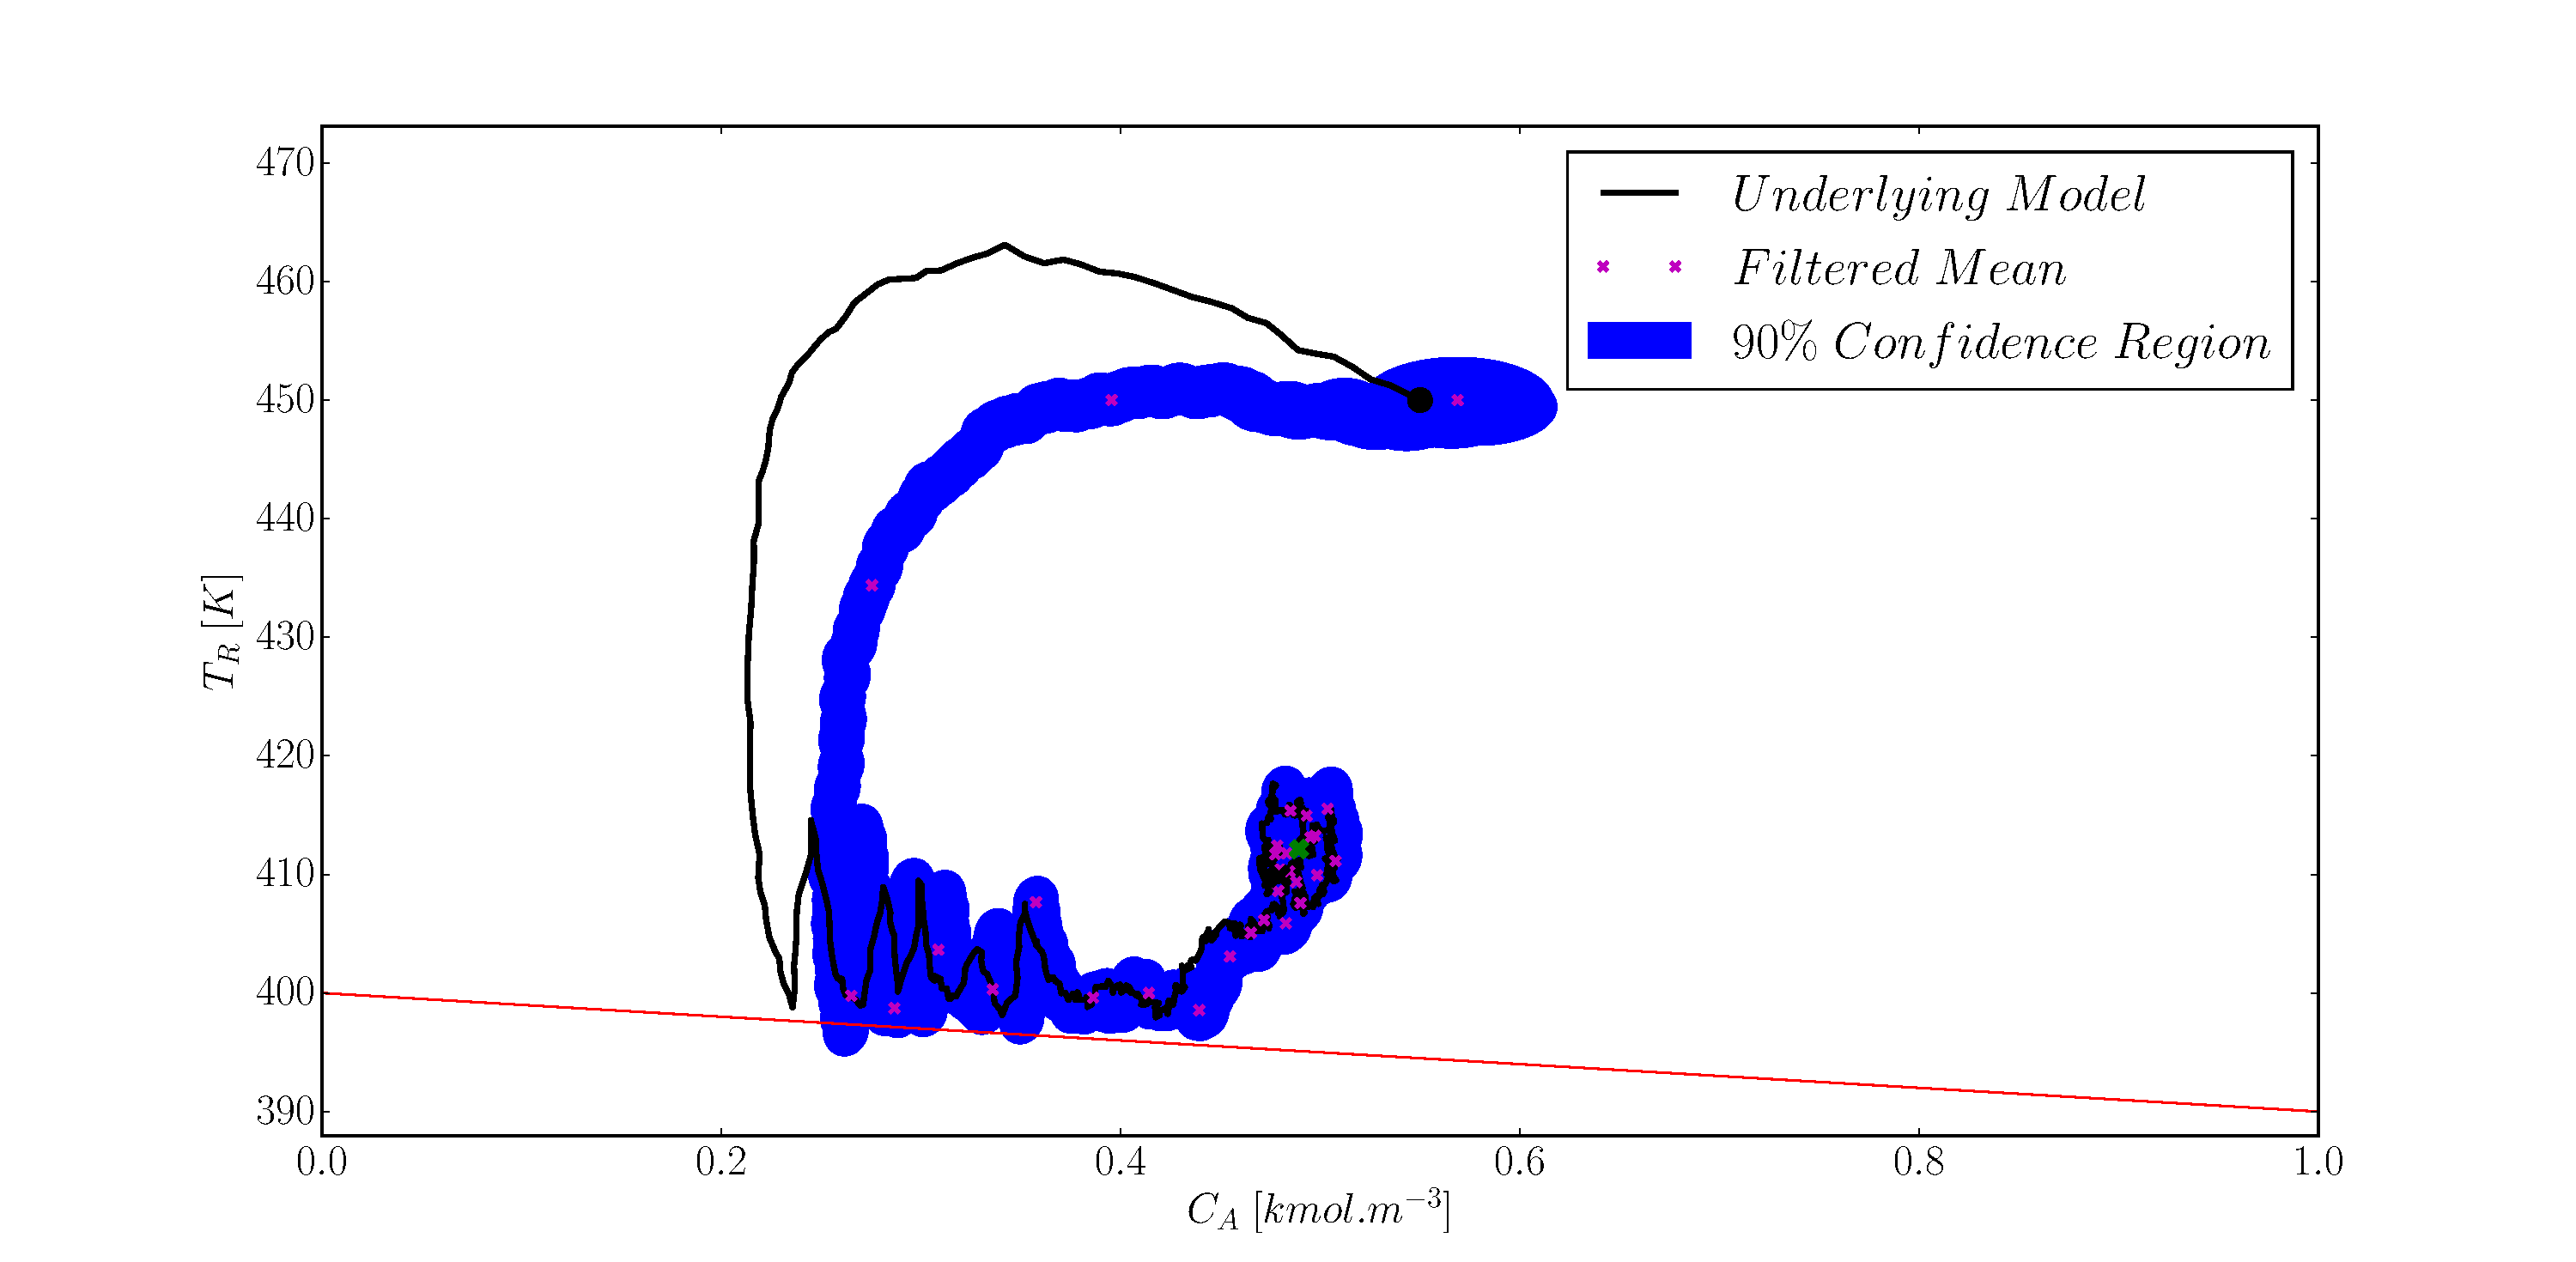
\includegraphics[scale=0.25]{nonlin_mod_kf_var90_ss.pdf}
\caption{Stochastic constrained MPC state space trajectory with initial condition $(0.55, 450)$ and measuring both states. A Kalman Filter is used for inference and the chance constraint is set at 90\%.}
\label{fig_nonlin_mod_kf_var90_ss}
\end{figure}
It is clear that the non-linearity of the underlying system makes stochastic control difficult. By increasing $k^2=13.8155$ which corresponds to changing the chance constraint such that $\text{Pr}(d^Tx_t + e \geq 0) \geq 99.9\% ~\forall ~t=1,...,N$ we hope to increase the minimum distance between the constraint and the underlying state.

Figure \ref{fig_nonlin_mod_kf_var999_track} shows the tracking of the modified system. The average energy input and average concentration error is 358 kJ/min and 11.31\% respectively. It is quite interesting that the more conservative system performs better with regard to these to metrics than the less conservative system.
\begin{figure}[H] 
\centering
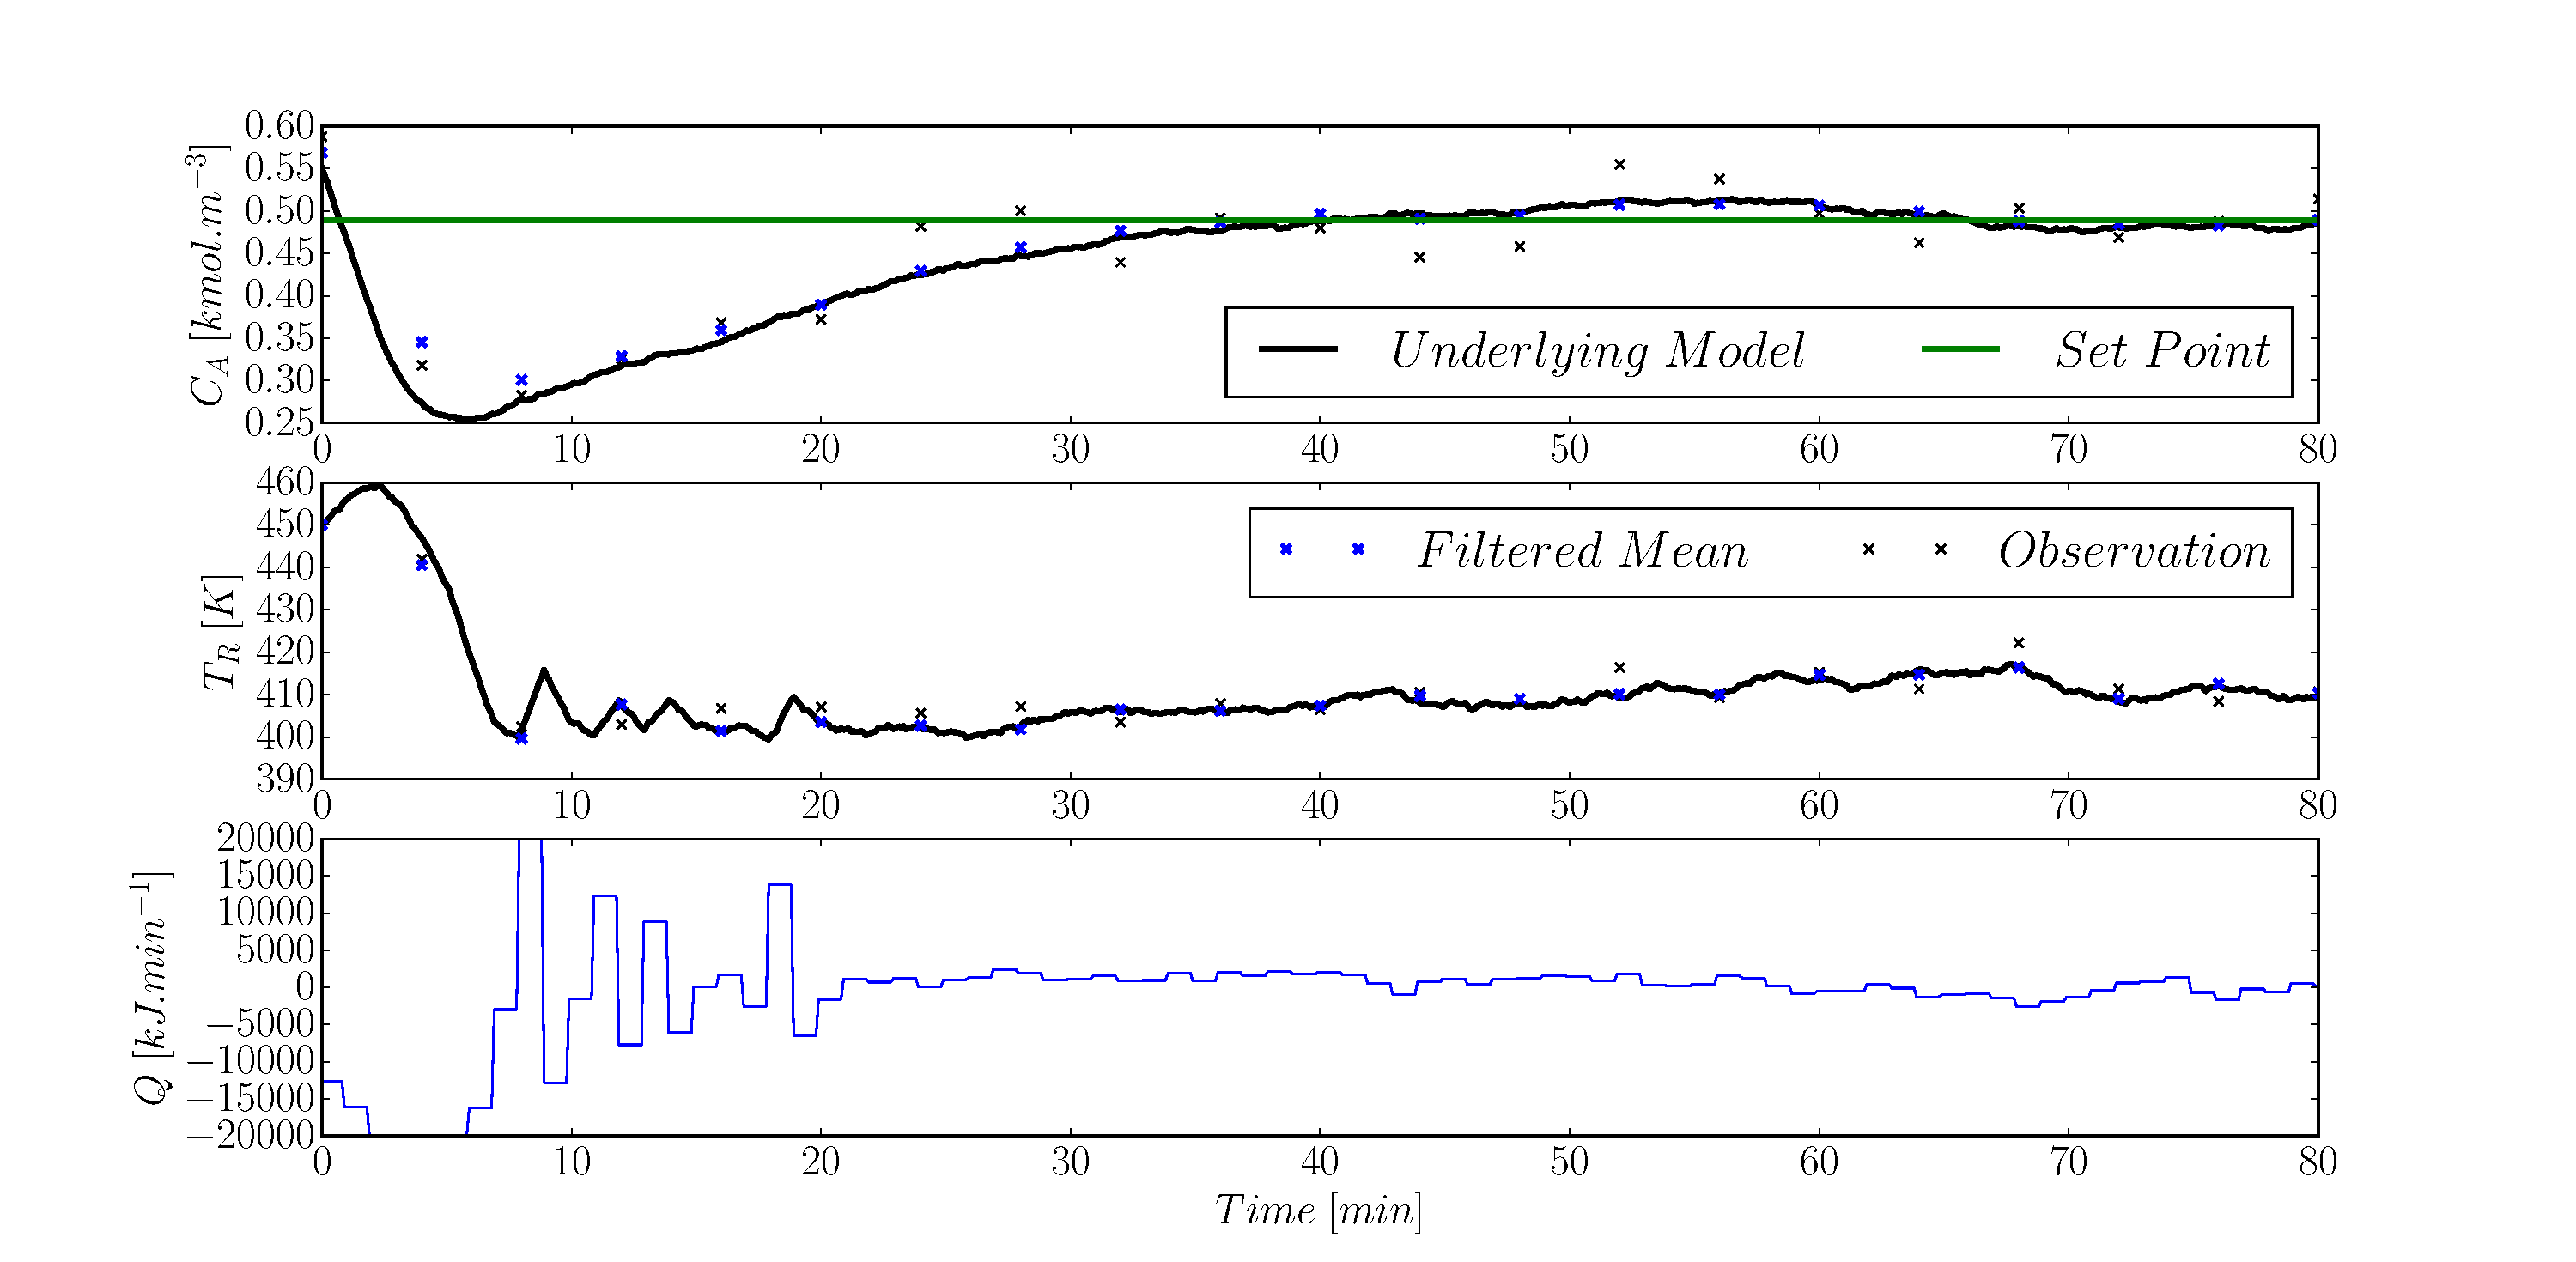
\includegraphics[scale=0.25]{nonlin_mod_kf_var999_track.pdf}
\caption{Stochastic constrained MPC tracking with initial condition $(0.55, 450)$ and measuring both states. A Kalman Filter is used for inference and the chance constraint is set at 99.9\%.}
\label{fig_nonlin_mod_kf_var999_track}
\end{figure}
In Figure \ref{fig_lin_mod_kf_var999_ss} we see that the margin of safety is increased although the confidence region still spills over the constraint.
\begin{figure}[H] 
\centering
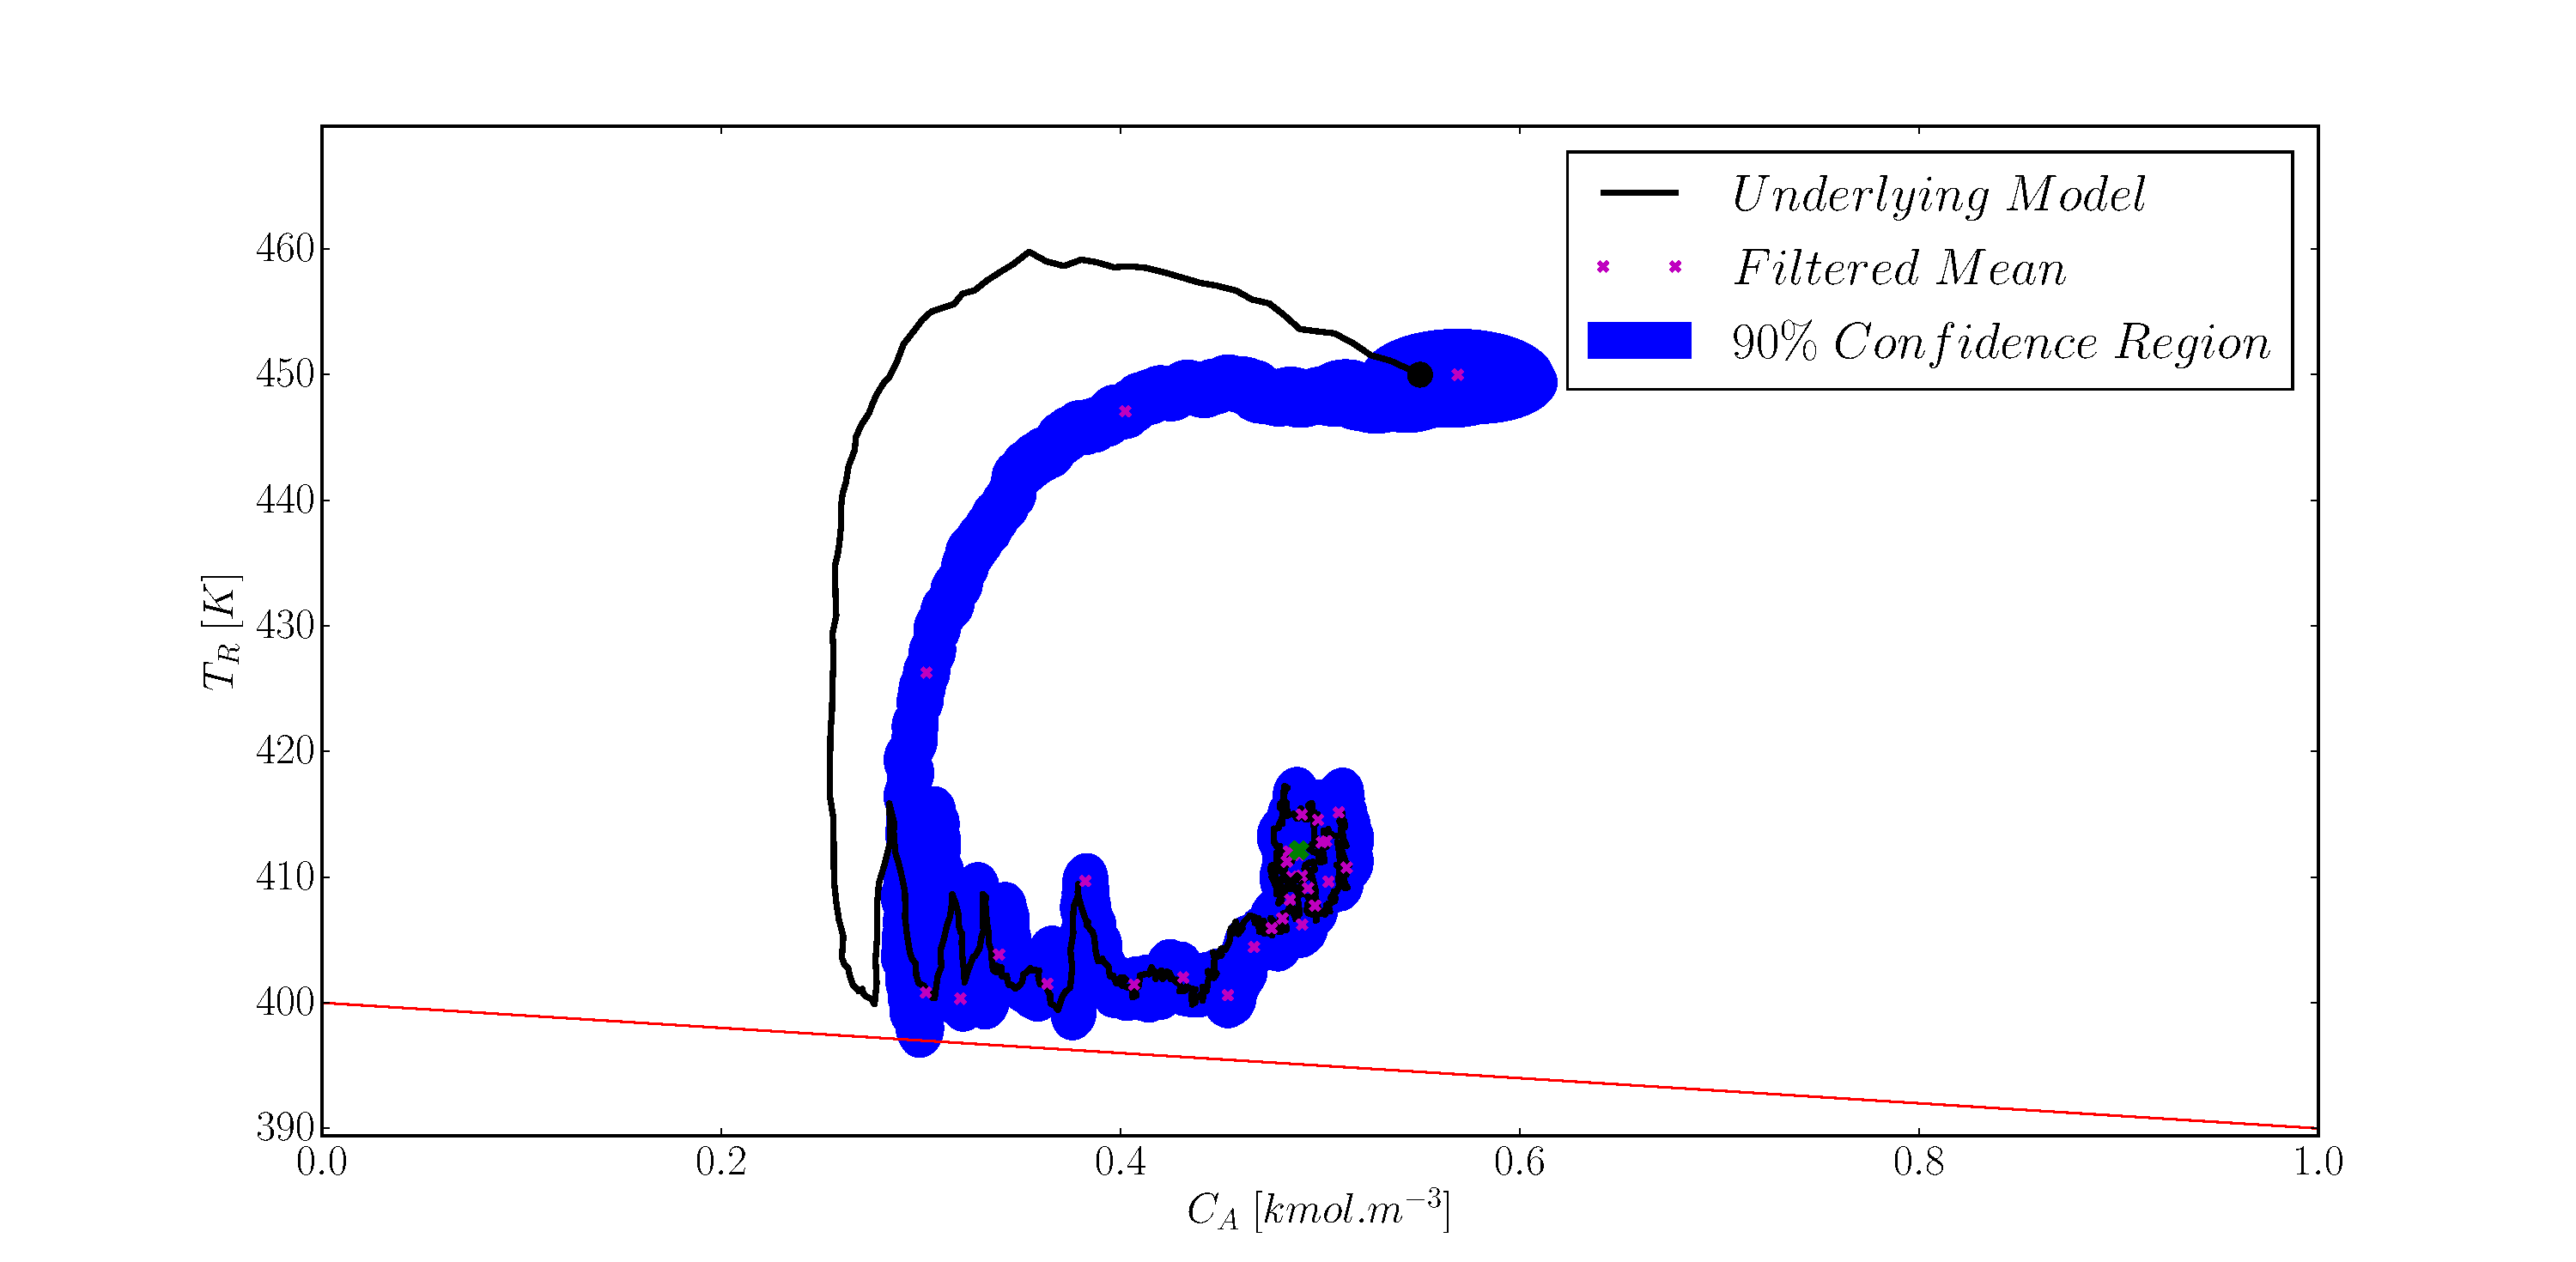
\includegraphics[scale=0.25]{nonlin_mod_kf_var999_ss.pdf}
\caption{Stochastic constrained MPC state space trajectory with initial condition $(0.55, 450)$ and measuring both states. A Kalman Filter is used for inference and the chance constraint is set at 99.9\%.}
\label{fig_nonlin_mod_kf_var999_ss}
\end{figure}
The ability of $k$ to increase or decrease the conservativeness of the constraint lends credibility to its value, at the very least if the system is non-normal, as an empirical measure to include stochastic robustness to the MPC in an efficient way.

Figures \ref{fig_nonlin_mod_kf_var90_track} to \ref{fig_nonlin_mod_kf_var999_ss} all display the undesirable property originally seen in Figure \ref{fig_nonlin_mod_kf_mean_track}: the poor state estimation and associated control problems. We attempt to rectify this situation by using a more sophisticated filter with the stochastic MPC. We use the MPC as shown in (\ref{eq_mpc_nonlin_mod_cons}) with a Particle filter using 200 particles. The tracking results are shown in Figure \ref{fig_nonlin_mod_pf_mean_track}. 
\begin{figure}[H] 
\centering
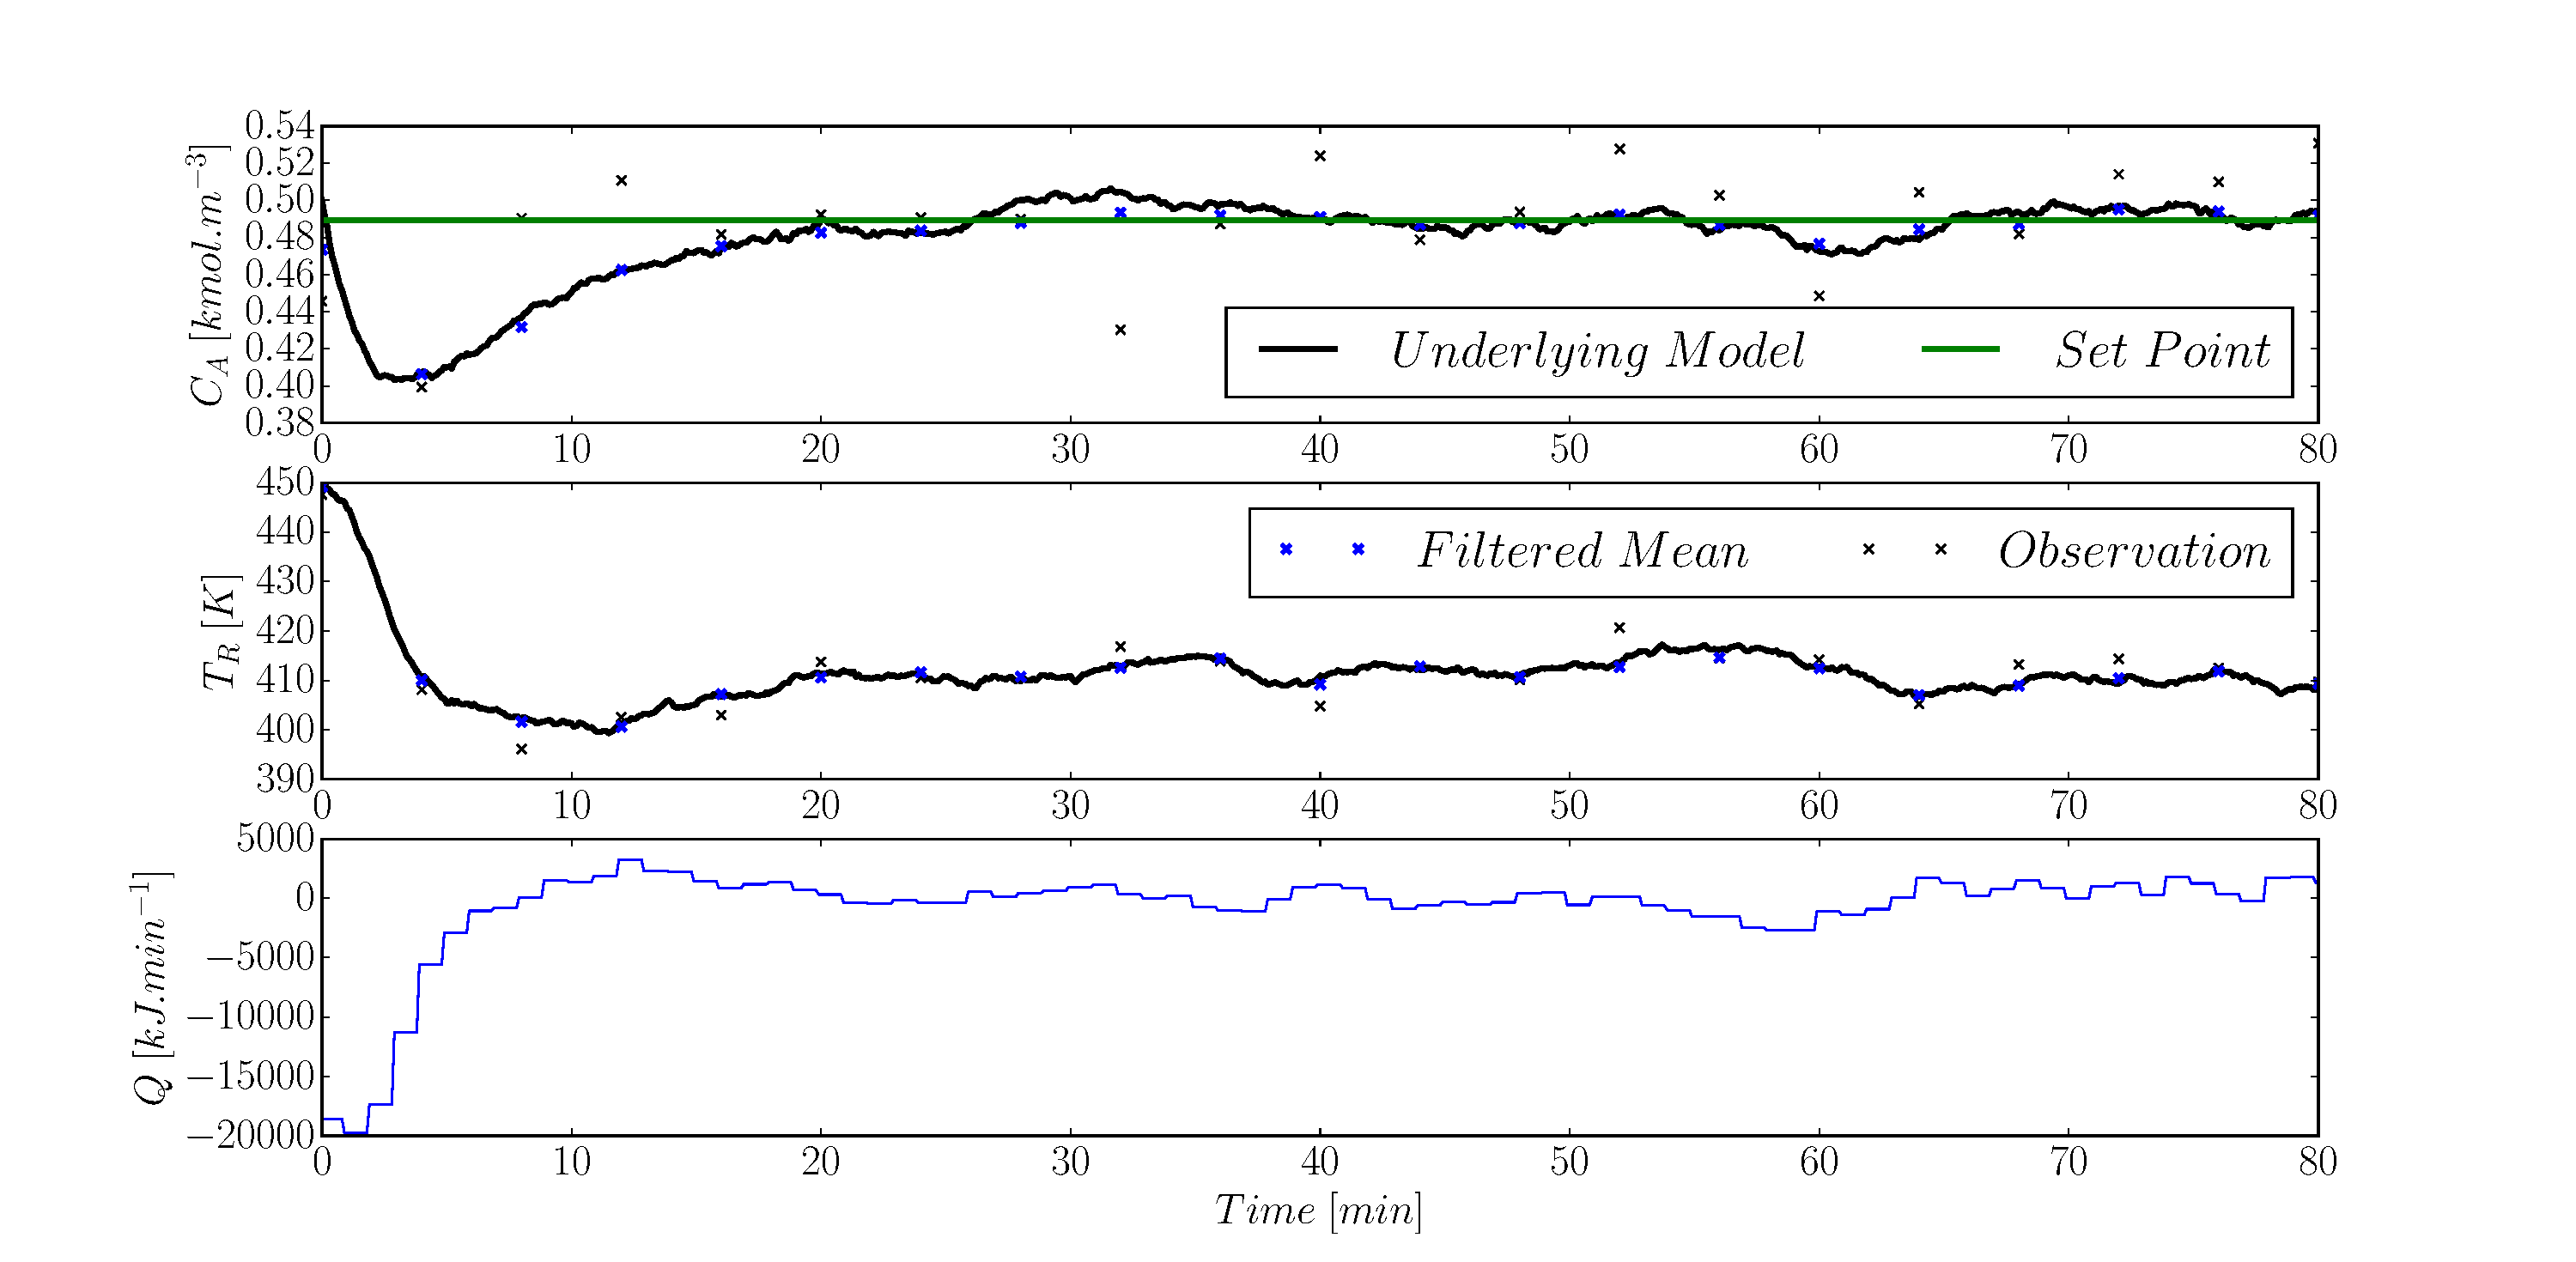
\includegraphics[scale=0.25]{nonlin_mod_pf_var90_track.pdf}
\caption{Stochastic constrained MPC tracking with initial condition $(0.55, 450)$ and measuring both states. A Particle Filter with 200 particles is used for inference and the chance constraint is set at 90\%.}
\label{fig_nonlin_mod_pf_var90_track}
\end{figure}
One could see the discussion in Section \ref{sec_nonlinmods_filtering} as a justification for using the Particle Filter instead of the Kalman Filter for state estimation. Since the underlying model is non-linear we expect the Particle Filter to outperform the Kalman Filter (recall the discussion following Figure \ref{fig_pf_kf_phase2}).

The average input energy and average concentration error is 178 kJ/min and 2.98\% over the course of the simulation. This is a vast improvement over the Kalman Filter MPC combination. Clearly the more accurate state estimation is immensely beneficial for control.

Figure \ref{fig_nonlin_mod_pf_var90_ss} also illustrates that the stochastic constraint is easily satisfied using the more accurate estimator.
\begin{figure}[H] 
\centering
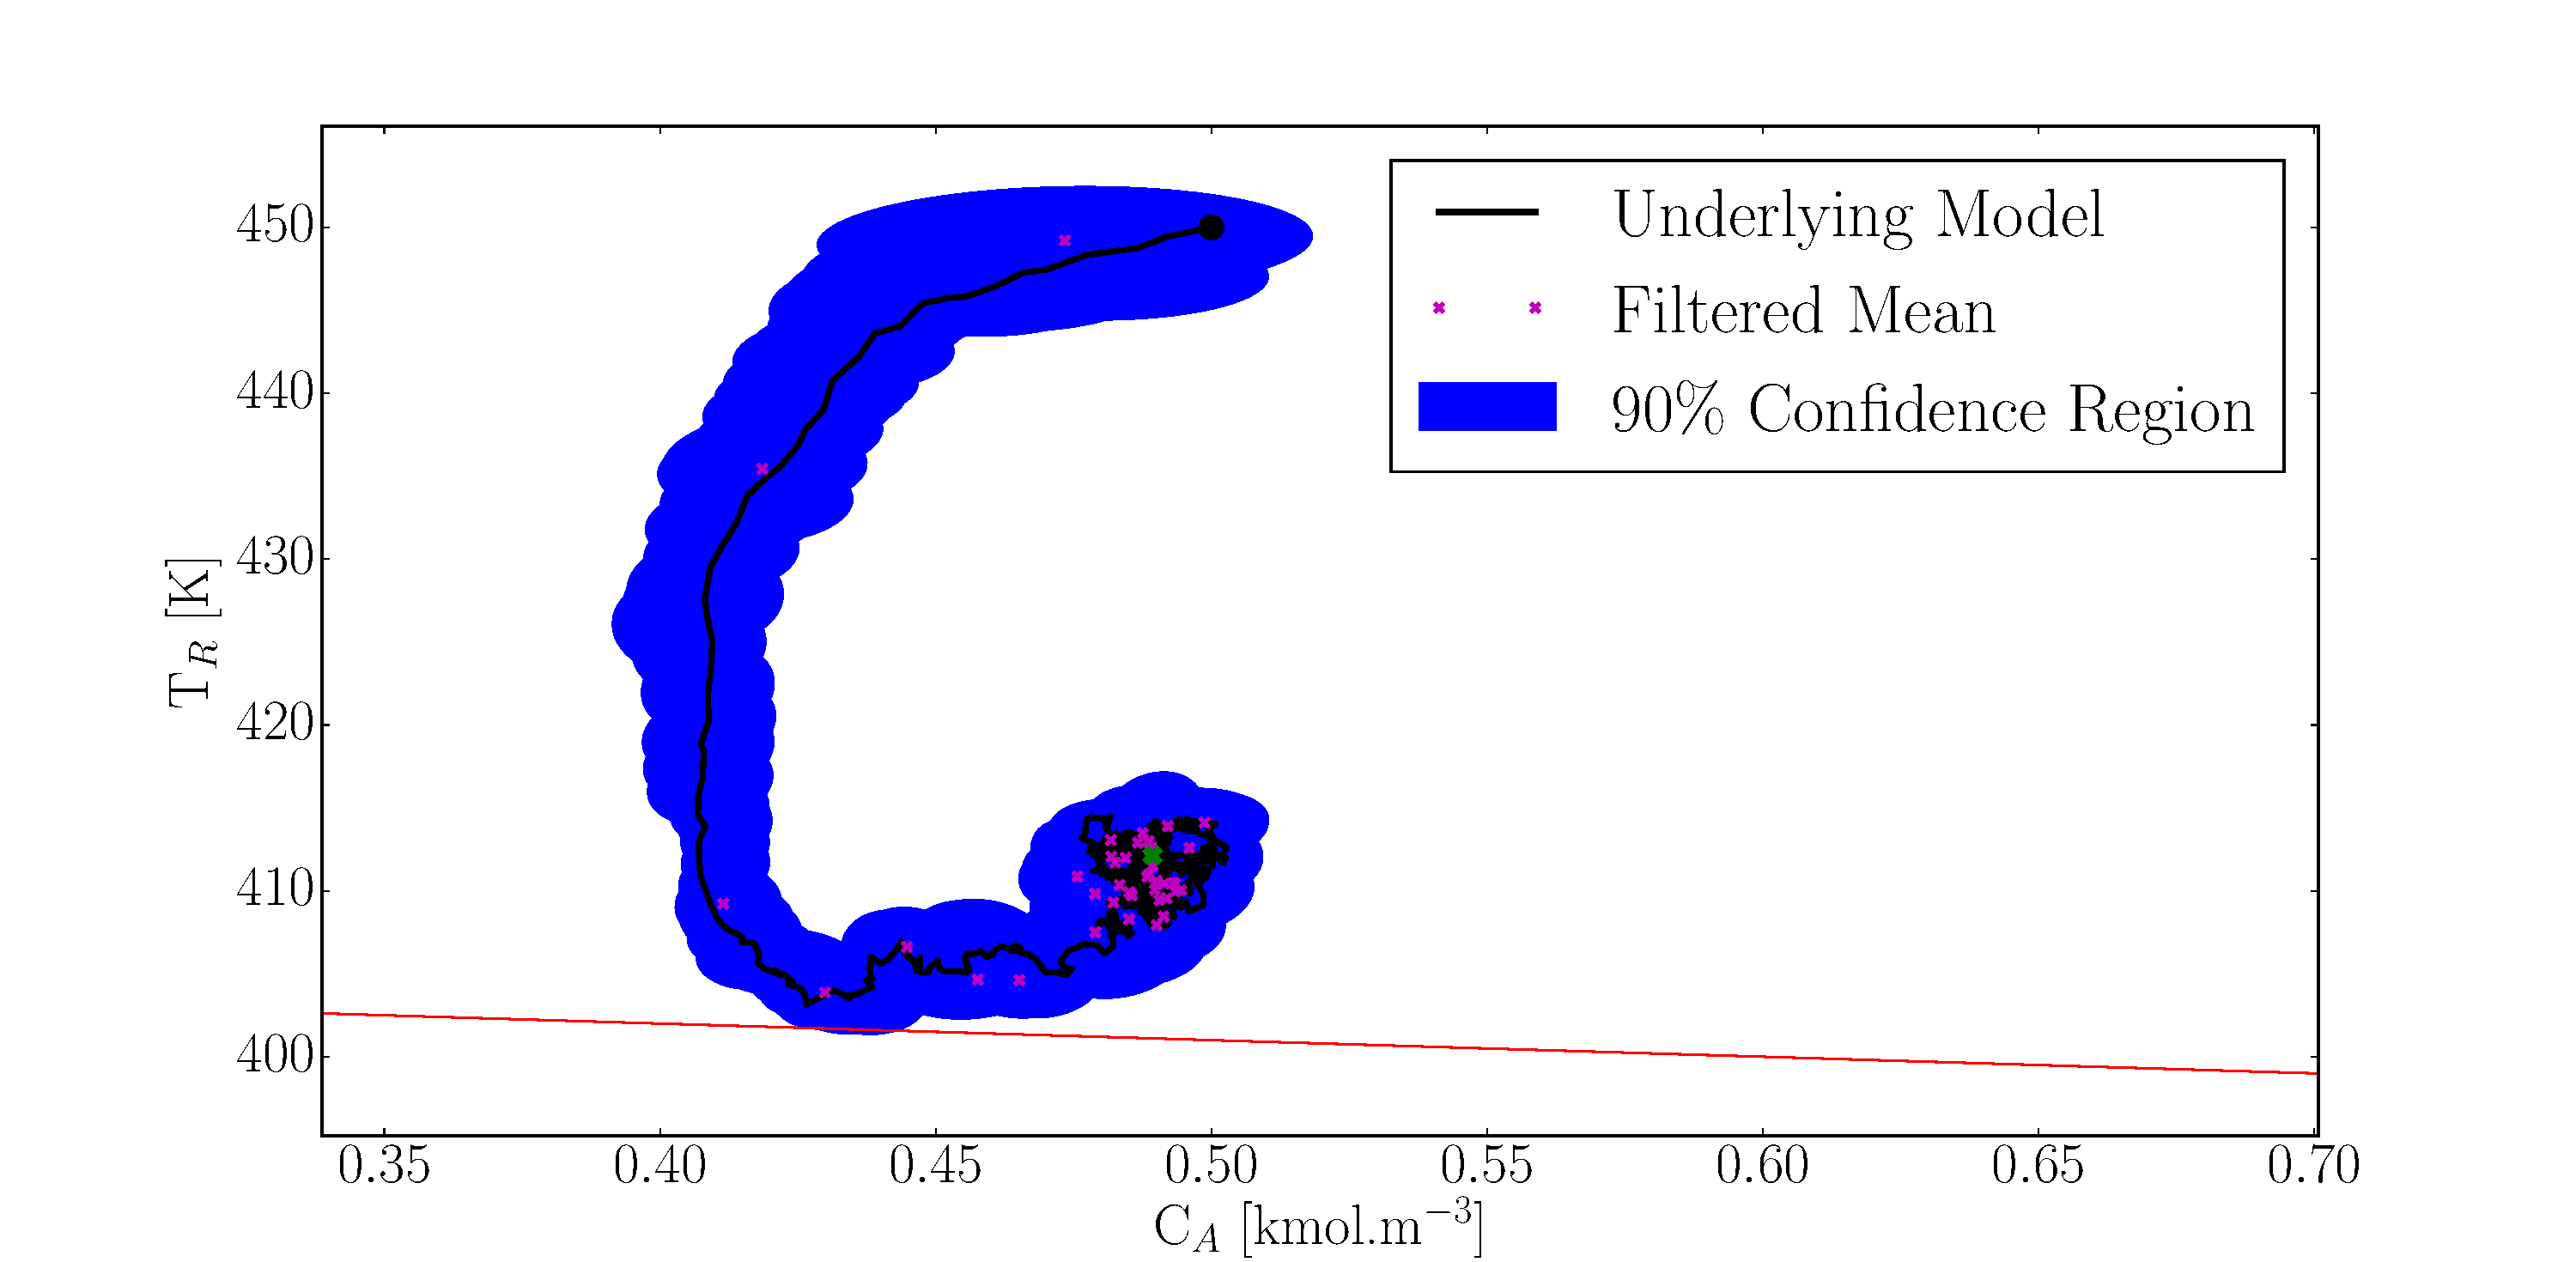
\includegraphics[scale=0.25]{nonlin_mod_pf_var90_ss.pdf}
\caption{Stochastic constrained MPC state space trajectory with initial condition $(0.55, 450)$ and measuring both states. A Particle Filter with 200 particles is used for inference and the chance constraint is set at 90\%.}
\label{fig_nonlin_mod_pf_var90_ss}
\end{figure}
As before we need to investigate the normal assumption underpinning the theory behind the chance constraint simplification. We investigate it in exactly the same manner as Figure \ref{fig_lin_mod_kl} using Kullback-Leibler Divergence. To this end, Figure \ref{fig_nonlin_mod_kl} shows the degree to which the underlying posterior state distributions are Gaussian given the non-linear underlying system.
\begin{figure}[H] 
\centering
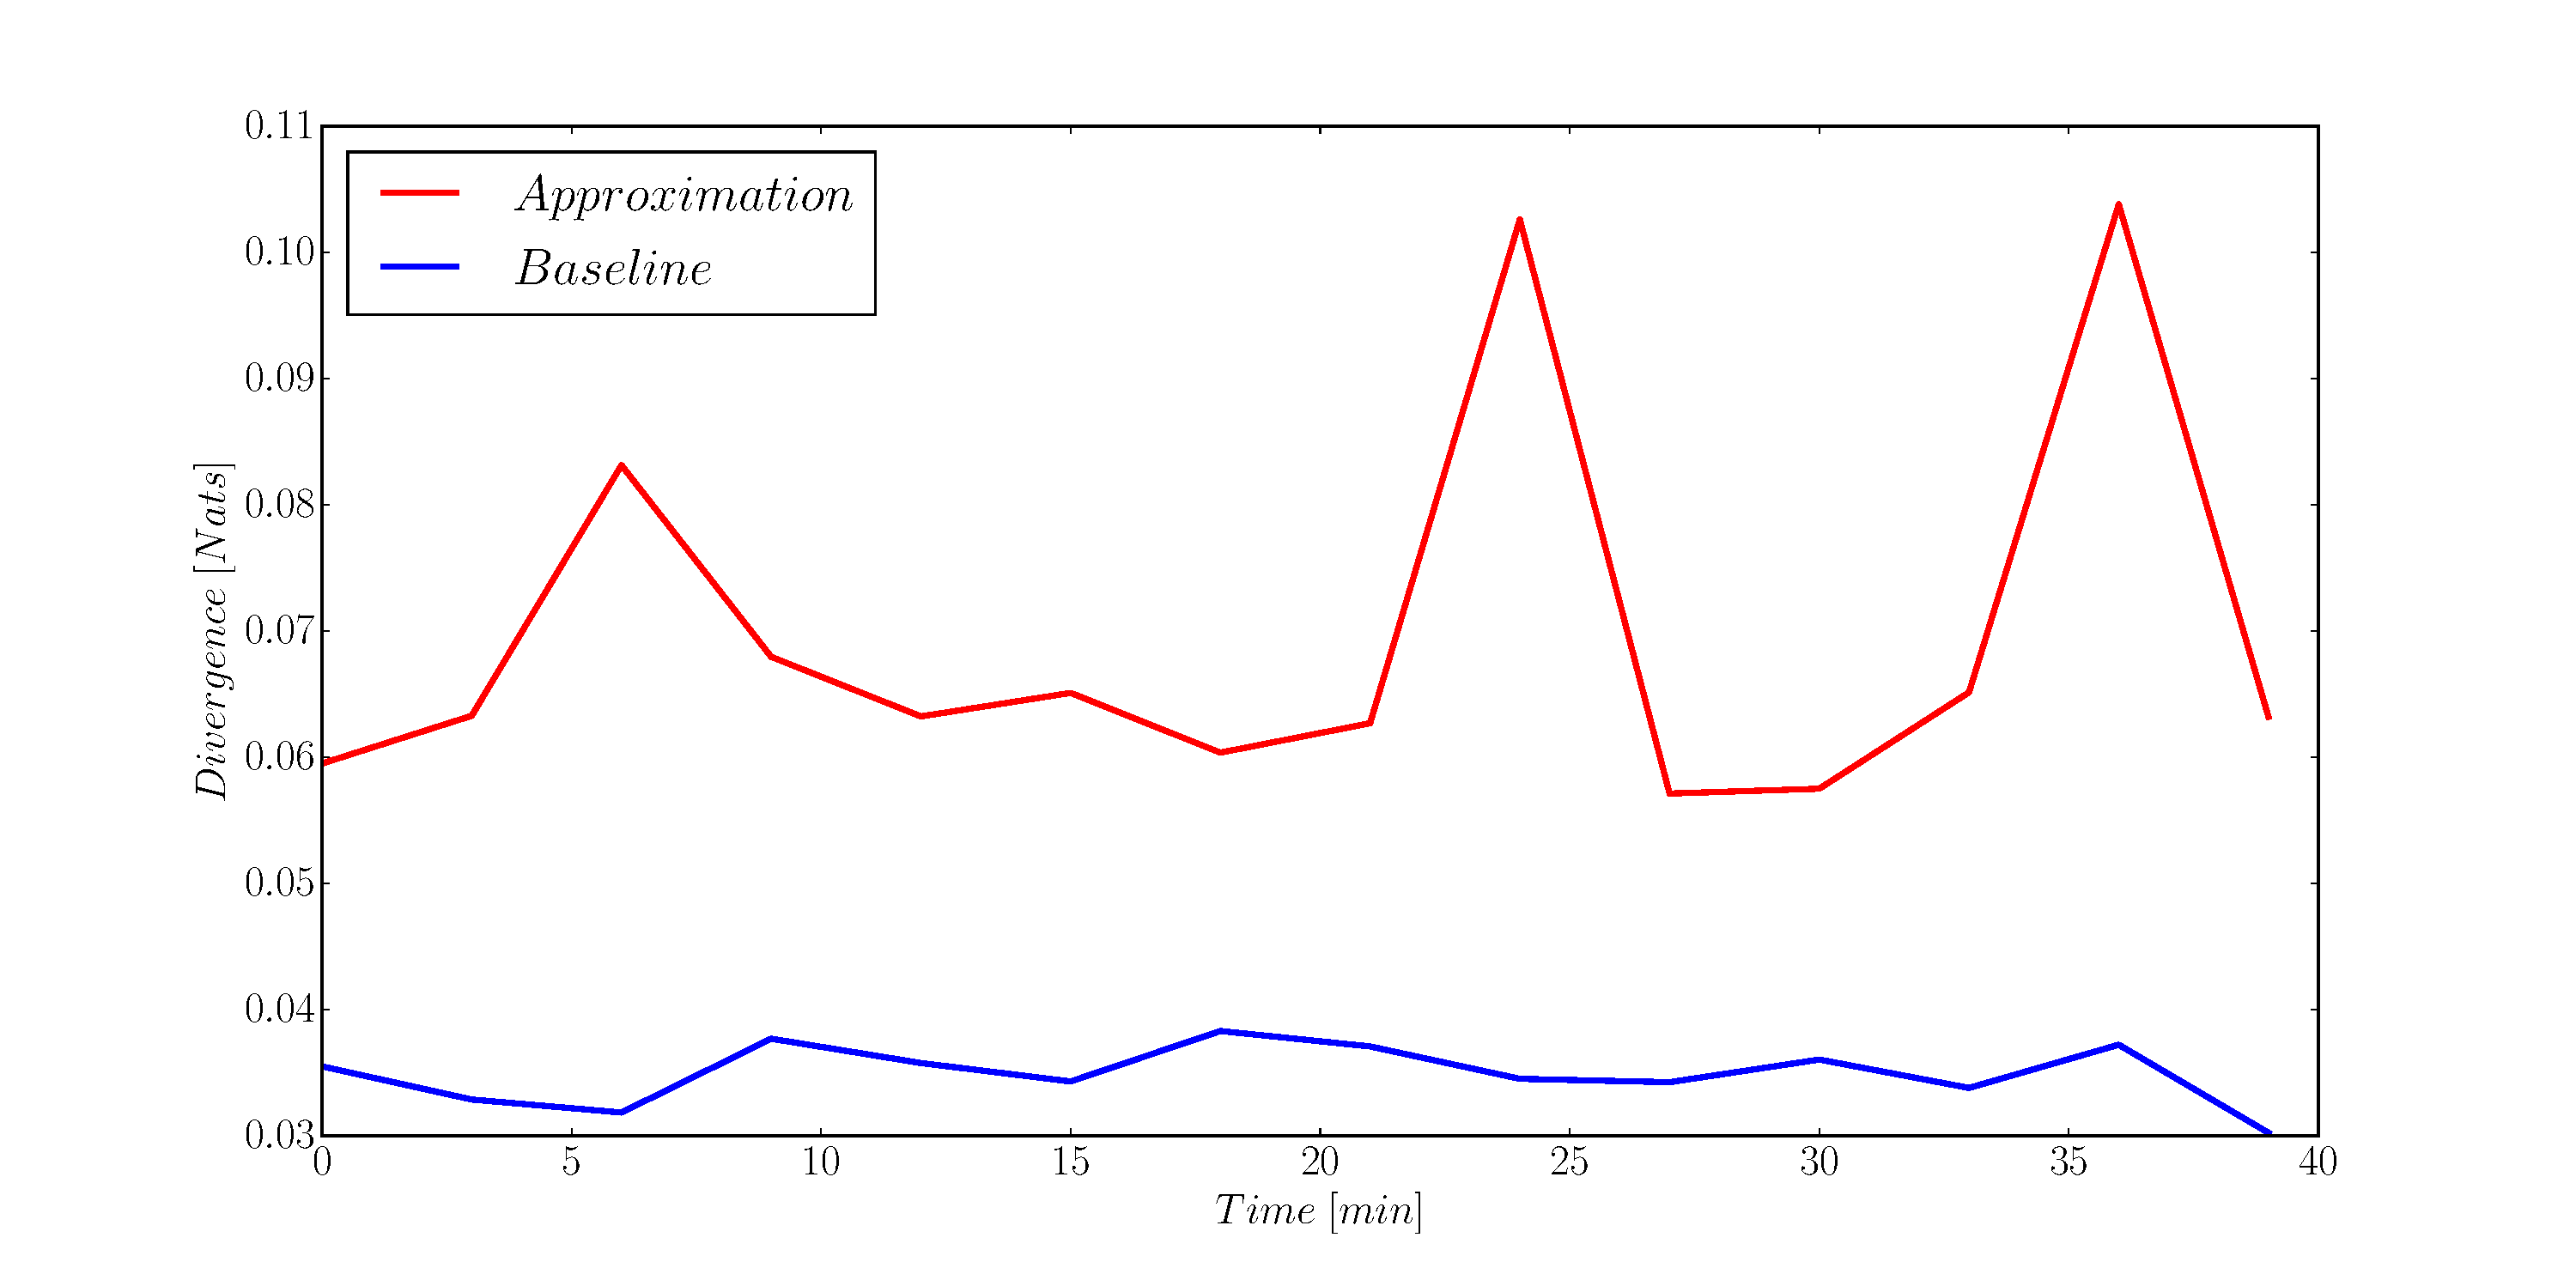
\includegraphics[scale=0.25]{nonlin_mod_kl.pdf}
\caption{Kullback-Leibler Divergence between the assumed Gaussian distribution and actual distribution using 5000 particles. The underlying model is non-linear.}
\label{fig_nonlin_mod_kl}
\end{figure}
It is a relief that the normal assumption seems to hold almost as well in the non-linear underlying system case. The average divergence for the baseline, approximation and uniform curves are: $0.035$, $0.071$ and $110.11$. It is not surprising that the non-linearity reduced the degree of normality of the distributions although it did not do so significantly. Therefore we can conclude that the normal assumption holds approximately.

\subsection{Conclusion}
We have illustrated the benefits gained by designing MPC within the framework of Probabilistic Graphical Models by showing:
\begin{enumerate}
\item
Under the assumption of normality and linearity it is possible to convert stochastic objective functions into their deterministic equivalents. The analysis is closely related to the work of \cite{yan1} and \cite{yan2} but we have shown that these results are immediately obvious from within the framework of Probabilistic Graphical Models. Thus it is possible to solve LQG objective type problems without resorting to stochastic Dynamic Programming.
\item
We have generalised our analysis to stochastic MPC and shown that by using the statistically important metric, the Mahalanobis Distance, we arrive at a technique for enforcing chance constraints which is very closely related to the approach taken by \cite{vanhessem2} and \cite{vanhessem1}. Under the assumptions of linearity and normality we have shown that constraint satisfaction is ensured. Due to the use of the Mahalanobis Distance metric we have provided some theoretical support for the use of the ``ellipsoidal approximation" technique if the underlying system is non-linear or not exactly Gaussian.
\item
Combining the previous results we have shown that it is possible to write the joint chance constrained stochastic MPC problem as a deterministic MPC problem. Additionally we show that the joint chance constraints can be written in a linear format. The entire optimisation problem can then be written in the standard form for Quadratic Programming optimisation. Standard deterministic MPC solution techniques can then be used to solve the stochastic problem.
\item
We have compared the effect different inference techniques have on the quality of the MPC. If the system is linear and Gaussian the Kalman Filter is adequate. If there is significant departure from linearity or normality it can be beneficial to use the Particle Filter.
\end{enumerate}
\chapter{Inference using Linear Hybrid Models}
In this section we generalise the Probabilistic Graphical Models of the previous sections as shown in Figure \ref{fig_hybridmod1}. We include the discrete random variables, $(s_0,s_1, s_2,...)$ where each variable has $M$ states, which we will call the switching variables. The goal of adding switching variables is to allow our graphical models to switch (or more precisely, choose based on the observation) between $M$ different dynamical models. For the moment we restrict ourselves to linear transition functions i.e. we use linear state space models. The other variables retain their meaning as before. Models of this form are usually called Switching Kalman Filter models \cite{murphy1}. 
\begin{figure}[H] 
\centering
\begin{tikzpicture}

  % Define nodes
  \node[obs] (ya) {$y_0$};
  \node[obs, right=of ya] (yb) {$y_1$};
  \node[obs, right=of yb] (yc) {$y_2$};
  \node[latent, above=of ya]  (xa) {$x_0$};
  \node[latent, above=of yb, right=of xa]  (xb) {$x_1$};
  \node[latent, above=of yc, right=of xb]  (xc) {$x_2$};
  \node[det, above=of xa, xshift=0.7cm] (da) {$u_0$};
  \node[det, above=of xb, xshift=0.7cm] (db) {$u_1$};
  \node[latent, above=of xa, yshift=1.1cm] (sa) {$s_0$};
  \node[latent, above=of xb, yshift=1.1cm] (sb) {$s_1$};
  \node[latent, above=of xc, yshift=1.1cm] (sc) {$s_2$};
  
  % Connect the nodes
  \edge {da} {xb};
  \edge {db} {xc};
  \edge {xa} {ya};
  \edge {xb} {yb};
  \edge {xc} {yc};
  \edge {xa} {xb};
  \edge {xb} {xc};
  \edge {sa} {sb};
  \edge {sb} {sc};
  \edge {sa} {xa};
  \edge {sb} {xb};
  \edge {sc} {xc};
  
\end{tikzpicture}
\caption{Graphical model of this section}
\label{fig_hybridmod1}
\end{figure}
One of the benefits of combining discrete switching variables with linear dynamical models is that it allows us to model nonlinear, even multi-modal, processes with linear models. Intuitively, we can glue together linear models which each describe a nonlinear model in some region and use the switch to determine which one to use. The switch assigns a weight to each model based on its ability to explain the evidence. 

We model this system as follows. Let $s_t \in (1,2,..., M)$ denote a discrete, time homogeneous $M$ state first order Markov chain with transition matrix $P$ as discussed in Section \ref{sec_hmm}. Let each state $s_t=i$ be associated with a parameter set $\left(A_i, B_i, W_i, C_i, V_i \right)$ used to evaluate the dynamical model shown in (\ref{eq_smodel}). If $s_t$ were observed then (\ref{eq_smodel}) would simplify to a set of Latent Linear Dynamical Systems we could perform inference on using the methods investigated in Section \ref{sec_inf_lin_mods}. However, we assume that $s_t$ is a hidden random variable.
\begin{equation}
\begin{aligned}
x_{t+1} &= A_ix_t + B_iu_t + w_{t} \text{ with } \mathcal{N}(w_{t}|0,W_i) \\
y_{t+1} &= C_ix_{t+1} + v_{t+1}  \text{ with } \mathcal{N}(v_{t+1}|0,V_i)
\end{aligned}
\label{eq_smodel}
\end{equation}
To fully specify the system we also require the prior distributions $p(s_0)$ and $p(x_0|s_0)$ as well as the switch transition matrix $P$. For the purposes of this dissertation we assumed that the switch transition matrix is available. This matrix can be inferred using the Baum-Welch Algorithm or it can be set using operator expertise as we will show later.

\section{Exact Filtering}
The switching variables ($s_0, s_1, s_2,...$) are discrete random variables exactly like the ones seen in Section \ref{sec_hmm}. There we derived recursive analytic expressions for inference which were computationally inexpensive. The structure of the stochastic variables ($x_0, x_1,x_2,...$) and ($y_0,y_1, y_2,...$) are exactly the same as those found Section \ref{sec_inf_lin_mods}. There we derived the famous Kalman Filter equations which were also analytic, recursive and computationally inexpensive. Taking this into consideration, it seems plausible to believe that inference, specifically filtering, for hybrid systems like (\ref{eq_smodel}) can be formulated in a computationally feasible manner. 

Unfortunately, it can be shown that this is not possible in general \cite{lerner}\cite{murphy3} because the memory requirements scale exponentially with time. Loosely speaking one can see this by noting that at the first time step the system is described by a weighted set of $M$ Kalman Filter models (due to the linear assumption and the $M$ switching indices). At time step two the system is described by a weighted set of $M^2$ Kalman Filter models. Continuing in this manner we see that at time step $t$ the memory requirement is $M^t$. Clearly this is computationally infeasible and calls for approximate methods to be used. 

In literature many approximate filtering algorithms exist and it is not clear which is best. Two of the more popular methods include Gaussian Sum Filtering \cite{barber2} and Particle Filtering based methods (specifically the Rao-Blackwellisation approach, see \cite{chen}\cite{doucet}). Both of these methods take advantage of the Gaussian structure of the system and operate in a fixed memory space making them computationally attractive. We focus on Particle based methods because it can be extended to nonlinear systems with ease.   

\section{Rao-Blackwellised Particle Filter}
It is our objective to find the joint posterior distribution $p(s_{0:t}, x_{0:t}|y_{0:t})$. This joint posterior admits filtering of Figure \ref{fig_hybridmod1} if we discard the trajectory and focus only on $s_t,x_t$. By the chain rule (Definition \ref{def_chain_rule_bayes}) we immediately have that $p(s_{0:t}, x_{0:t}|y_{0:t}) = p(s_{0:t}|y_{0:t})p(x_{0:t}|y_{0:t}, s_{0:t})$. Given $s_{0:t}$ we see that $p(x_{0:t}|y_{0:t}, s_{0:t})$ can be evaluated using the Kalman Filter equations (see Section \ref{sec_inf_lin_mods}) and thus we are only concerned with finding some approximation for $p(s_{0:t}|y_{0:t})$. This is the essence of the Rao-Blackwellised Particle Filter - taking advantage of the conditionally linear Gaussian nature of the system to analytically evaluate a part of the posterior distribution \cite{doucet}.

Using the formulation of the adaptive Sequential Importance Sampling algorithm discussed in Section \ref{sec_inf_nonlin_mods} we can apply it to find an approximation of $p(s_{0:t}|y_{0:t})$. We set $\gamma_t(s_{0:t})=p(s_{0:t},y_{0:t})$ and $Z_t=p(y_{0:t})$ and then have that $\frac{\gamma_t(s_{0:t})}{Z_t} = p(s_{0:t}|y_{0:t})$ as desired. We then choose our proposal distribution $q_t(s_{0:t}|y_{0:t})$ to be recursive and follow the same procedure as before, shown in (\ref{eq_rbweight1}).
\begin{equation}
\begin{aligned}
w_t(s_{0:t}) &= \frac{\gamma_t(s_{0:t},y_{0:t})}{q_t(s_{0:t}|y_{0:t})} \\
&= \frac{p(s_{0:t},y_{0:t})}{q_t(s_{0:t}|y_{0:t})} \\
&\propto \frac{p(s_{0:t}|y_{0:t})}{q_t(s_{0:t}|y_{0:t})} \\
&\propto \frac{p(y_t|s_t)p(s_t|s_{t-1})}{q_t(s_t|s_{0:t-1},y_{0:t})}\frac{p(s_{0:t-1}|y_{0:t-1})}{q_t(s_{0:t-1}|y_{0:t-1})} \\
&= \alpha_t(s_{0:t})w_{t-1}(s_{0:t-1})
\end{aligned}
\label{eq_rbweight1}
\end{equation}
As before, we are not interested in the whole trajectory of the switching variable because we only need to perform filtering. Thus our proposal distribution can be chosen to be the prior i.e. $q_t(s_t|s_{0:t-1},y_{0:t}) = p(s_t|s_{t-1})$. This is suboptimal but easy to sample from \cite{doucet}. The incremental weight then simplifies to $\alpha_t(s_{0:t}) = p(y_t|s_t)$. We can evaluate this distribution by marginalising out $x_t$ and using the properties of the Gaussian distributions as before (\ref{eq_rbweight2}).
\begin{equation}
\begin{aligned}
\alpha_t(s_{0:t}) &= p(y_t|s_t) \\
&= \int_{x_t} p(y_t|x_t,s_t)p(x_t|s_{0:t},y_{0:t-1}) \\
&= p(y_t|y_{0:t-1}, s_{0:t}) \\
&= \mathcal{N}\left(y_t | C_{s_t}A_{s_t}\mu_{t-1}, C_{s_t}\left(A_{s_t}\Sigma_{t-1}A_{s_t}^T+Q_{s_t} \right)C_{s_t} + R_{s_t} \right)
\end{aligned}
\label{eq_rbweight2}
\end{equation} 
Where the subscript $s_t$ denotes the state of the switching variable at time $t$ \cite{murphy1}. Upon inspection we see that (\ref{eq_rbweight2}) is just the one step ahead prediction likelihood as discussed in Section \ref{sec_lin_prediction} \cite{murphy1}. Note that we will still need to resample the switching state from $P$ periodically to prevent sample impoverishment. 

We now have an efficient particle approximation of $p(s_t|y_t)$. To find the filtered posterior distribution as desired we note that $p(s_t,x_t|y_{0:t}) = \sum_i w_t(S_t^i)\delta(S_t^i, s_t)p(x_t|y_{0:t}, S_t^i)$ where $S_t^i$ is the i$^{\text{th}}$ particle. Each particle thus consists of a weight, a switch sample and the sufficient statistics generated by the Kalman Filter for a Gaussian i.e. a mean and covariance. The complete algorithm is shown below.

\textbf{Rao-Blackwellised Particle Filter Algorithm}\\
For $t=0$:
\begin{enumerate}
\item
Sample $S^i_0 \backsim p(s_0)$ and $\mu_{0|0}^i \backsim p(x_0|s_0)$.
\item
Compute the weights $w_0(S_0^i) = p(y_0|S_0^i)$ where $y_0$ is the observation. Normalise $W^i_0 \propto w_0(S^i_0)$.
\item
Apply the update step of the Kalman Filter to each particle $i$ and associated parameters to find $\mu_0^i$ and $\Sigma_0^i$. 
\item
If the number of effective particles is below some threshold apply resampling with roughening $(W^i_0, {S}^i_0,{\mu}^i_0, {\Sigma}^i_0)$ to obtain $N$ equally weighted particles $(\frac{1}{N}, \bar{S}^i_0, \bar{\mu}^i_0, \bar{\Sigma}^i_0)$ and set $(\bar{W}^i_0, \bar{S}^i_0, \bar{\mu}^i_0, \bar{\Sigma}^i_0) \leftarrow (\frac{1}{N}, \bar{S}^i_0, \bar{\mu}^i_0, \bar{\Sigma}^i_0)$ otherwise set $(\bar{W}^i_0, \bar{S}^i_0, \bar{\mu}^i_0, \bar{\Sigma}^i_0) \leftarrow ({W}^i_0, {S}^i_0, \mu^i_0, \Sigma_0^i)$
\end{enumerate}
For $t \geq 1$:
\begin{enumerate}
\item
Sample $S^i_t \backsim p(S_t^i|\bar{S}^i_{t-1})$.
\item
Compute the weights $\alpha_t(S^i_{t}) = p(y_t|S_t^i)$ and normalise $W^i_t \propto \bar{W}^i_{t-1}\alpha_t(S^i_{t})$.
\item
Apply the Kalman Filter algorithm to $\mu_{t-1}$ and $\Sigma_{t-1}$ for each particle $i$ to find the sufficient statistics $\mu_{t}$ and $\Sigma_{t}$ using the parameters corresponding to the state of $S^i_t$.
\item
If the number of effective particles is below some threshold apply resampling with roughening $(W^i_t, {S}^i_t,{\mu}^i_t, {\Sigma}^i_t)$ to obtain $N$ equally weighted particles $(\frac{1}{N}, \bar{S}^i_t, \bar{\mu}^i_t, \bar{\Sigma}^i_t)$ and set $(\bar{W}^i_t, \bar{S}^i_t, \bar{\mu}^i_t, \bar{\Sigma}^i_t) \leftarrow (\frac{1}{N}, \bar{S}^i_t, \bar{\mu}^i_t, \bar{\Sigma}^i_t)$ otherwise set $(\bar{W}^i_t, \bar{S}^i_t, \bar{\mu}^i_t, \bar{\Sigma}^i_t) \leftarrow ({W}^i_t, {S}^i_t, \mu^i_t, \Sigma_t^i)$
\end{enumerate} 

\section{Rao-Blackwellised Particle Prediction}
Like the Particle Predictor studied in the previous section, performing prediction using Rao-Blackwellisation is straightforward because there is no weighting (updating the particles based on the observation) step. Each particle's switching state is merely propagated forward using the proposal distribution (the transition matrix $P$) and the Kalman prediction algorithm is used to evaluate the predicted mean and covariance. For the sake of brevity we do not supply an algorithm because it is a straightforward simplification of the Rao-Blackwellised Particle Filter Algorithm as shown above. The corresponding Probabilistic Graphical Model is shown in Figure \ref{fig_hybridmod1_prediction}.
\begin{figure}[H] 
\centering
\begin{tikzpicture}

  % Define nodes
  \node[obs] (ya) {$y_0$};
  \node[latent, above=of ya]  (xa) {$x_0$};
  \node[latent, above=of yb, right=of xa]  (xb) {$x_1$};
  \node[latent, above=of yc, right=of xb]  (xc) {$x_2$};
  \node[det, above=of xa, xshift=0.7cm] (da) {$u_0$};
  \node[det, above=of xb, xshift=0.7cm] (db) {$u_1$};
  \node[latent, above=of xa, yshift=1.1cm] (sa) {$s_0$};
  \node[latent, above=of xb, yshift=1.1cm] (sb) {$s_1$};
  \node[latent, above=of xc, yshift=1.1cm] (sc) {$s_2$};
  
  % Connect the nodes
  \edge {da} {xb};
  \edge {db} {xc};
  \edge {xa} {ya};
  \edge {xa} {xb};
  \edge {xb} {xc};
  \edge {sa} {sb};
  \edge {sb} {sc};
  \edge {sa} {xa};
  \edge {sb} {xb};
  \edge {sc} {xc};
  
\end{tikzpicture}
\caption{Rao-Blackwellised Particle Prediction Graphical Model}
\label{fig_hybridmod1_prediction}
\end{figure}

\section{Smoothing and Viterbi Decoding}
It is also possible to take advantage of the Gaussian structure in Figure \ref{fig_hybridmod1} to derive a so-called Rao-Blackwellised Smoothing Algorithm. We do not include it here because it is not necessary for the purposes of this dissertation. We refer the reader to the relevant literature \cite{chen}\cite{doucet}. 

Viterbi decoding is likewise not within the scope of this dissertation and as such we refer the reader to \cite{murphy1} for more information. Suffice to say, by increasing the complexity of Figure \ref{fig_hybridmod1} we increase the difficulty of inference in general.

\section{Filtering the CSTR}
We now apply the Rao-Blackwellised Particle Filter (RBPF) to the CSTR introduced in Section \ref{sec_cstr}. The focus of this dissertation is on the application of Probabilistic Graphical Models to control, therefore our investigation into the various aspects which improve or degrade filtering performance will be relatively superficial and will target factors which are most relevant only. We will briefly investigate 3 aspects influencing the accuracy of the filter:
\begin{enumerate}
\item
The effect the switch transition matrix $P$ has on the filter.
\item
The effect using more models has on the filter.
\item
Using more state measurements.
\end{enumerate}
Like in Section \ref{sec_inf_nonlin_mods} we do not investigate the effect increasing the number of particles will have on inference. The same reasons apply and we use the same motivation in selecting the number of particles we use in this section.

It should be noted that in all the succeeding investigations only the most probably particle was used to estimate the current state. The reason for this will become clear in Section \ref{sec_rbpf_control} and \ref{sec_spf_control}. It is possible that more accurate state estimates could be reached by using a weighted average of the particles - this approach should be investigated further.

Note that we use the same parameters (e.g. noise covariances etc.) unless otherwise noted as used in Section \ref{sec_inf_lin_mods}.

We begin our investigation by only measuring temperature and using 3 linear models, derived by linearising the non-linear CSTR model at each nominal operating point. Since the CSTR has 3 nominal operating points we have 3 linear models. We compare the use of 2 different switch transition matrices $P_1$ and $P_2$ as shown in (\ref{eq_switch_trans}). The first index corresponds to the high temperature operating point ($M_1$), the second index to the unstable operating point ($M_2$) and the third index to the low temperature operating point ($M_3$).
\begin{equation}
\begin{aligned}
P_1 = \begin{pmatrix}
0.50 & 0.25 & 0.25 \\
0.25 & 0.50 & 0.25 \\
0.25 & 0.25 & 0.50
\end{pmatrix} 
~~~&P_2 = \begin{pmatrix}
0.99 & 0.01 & 0.00 \\
0.01 & 0.98 & 0.01 \\
0.00 & 0.01 & 0.99
\end{pmatrix}
\end{aligned}
\label{eq_switch_trans}
\end{equation}
Intuitively $P_1$ indicates that we are less sure about the underlying dynamical transitions i.e. we believe it is possible for the system to jump from the dynamics of the low temperature operating point to the dynamics of the high temperature operating point. Conversely, $P_2$ indicates that we believe it is impossible for the system dynamics to jump from the low temperature operating point to the high temperature operating point without first transitioning through the unstable operating point. 

Figure \ref{fig_3m_models} shows the state space trajectory of the system we are attempting to perform filtering on. The operating points (points of linearisation) are superimposed on the state space.
\begin{figure}[H] 
\centering
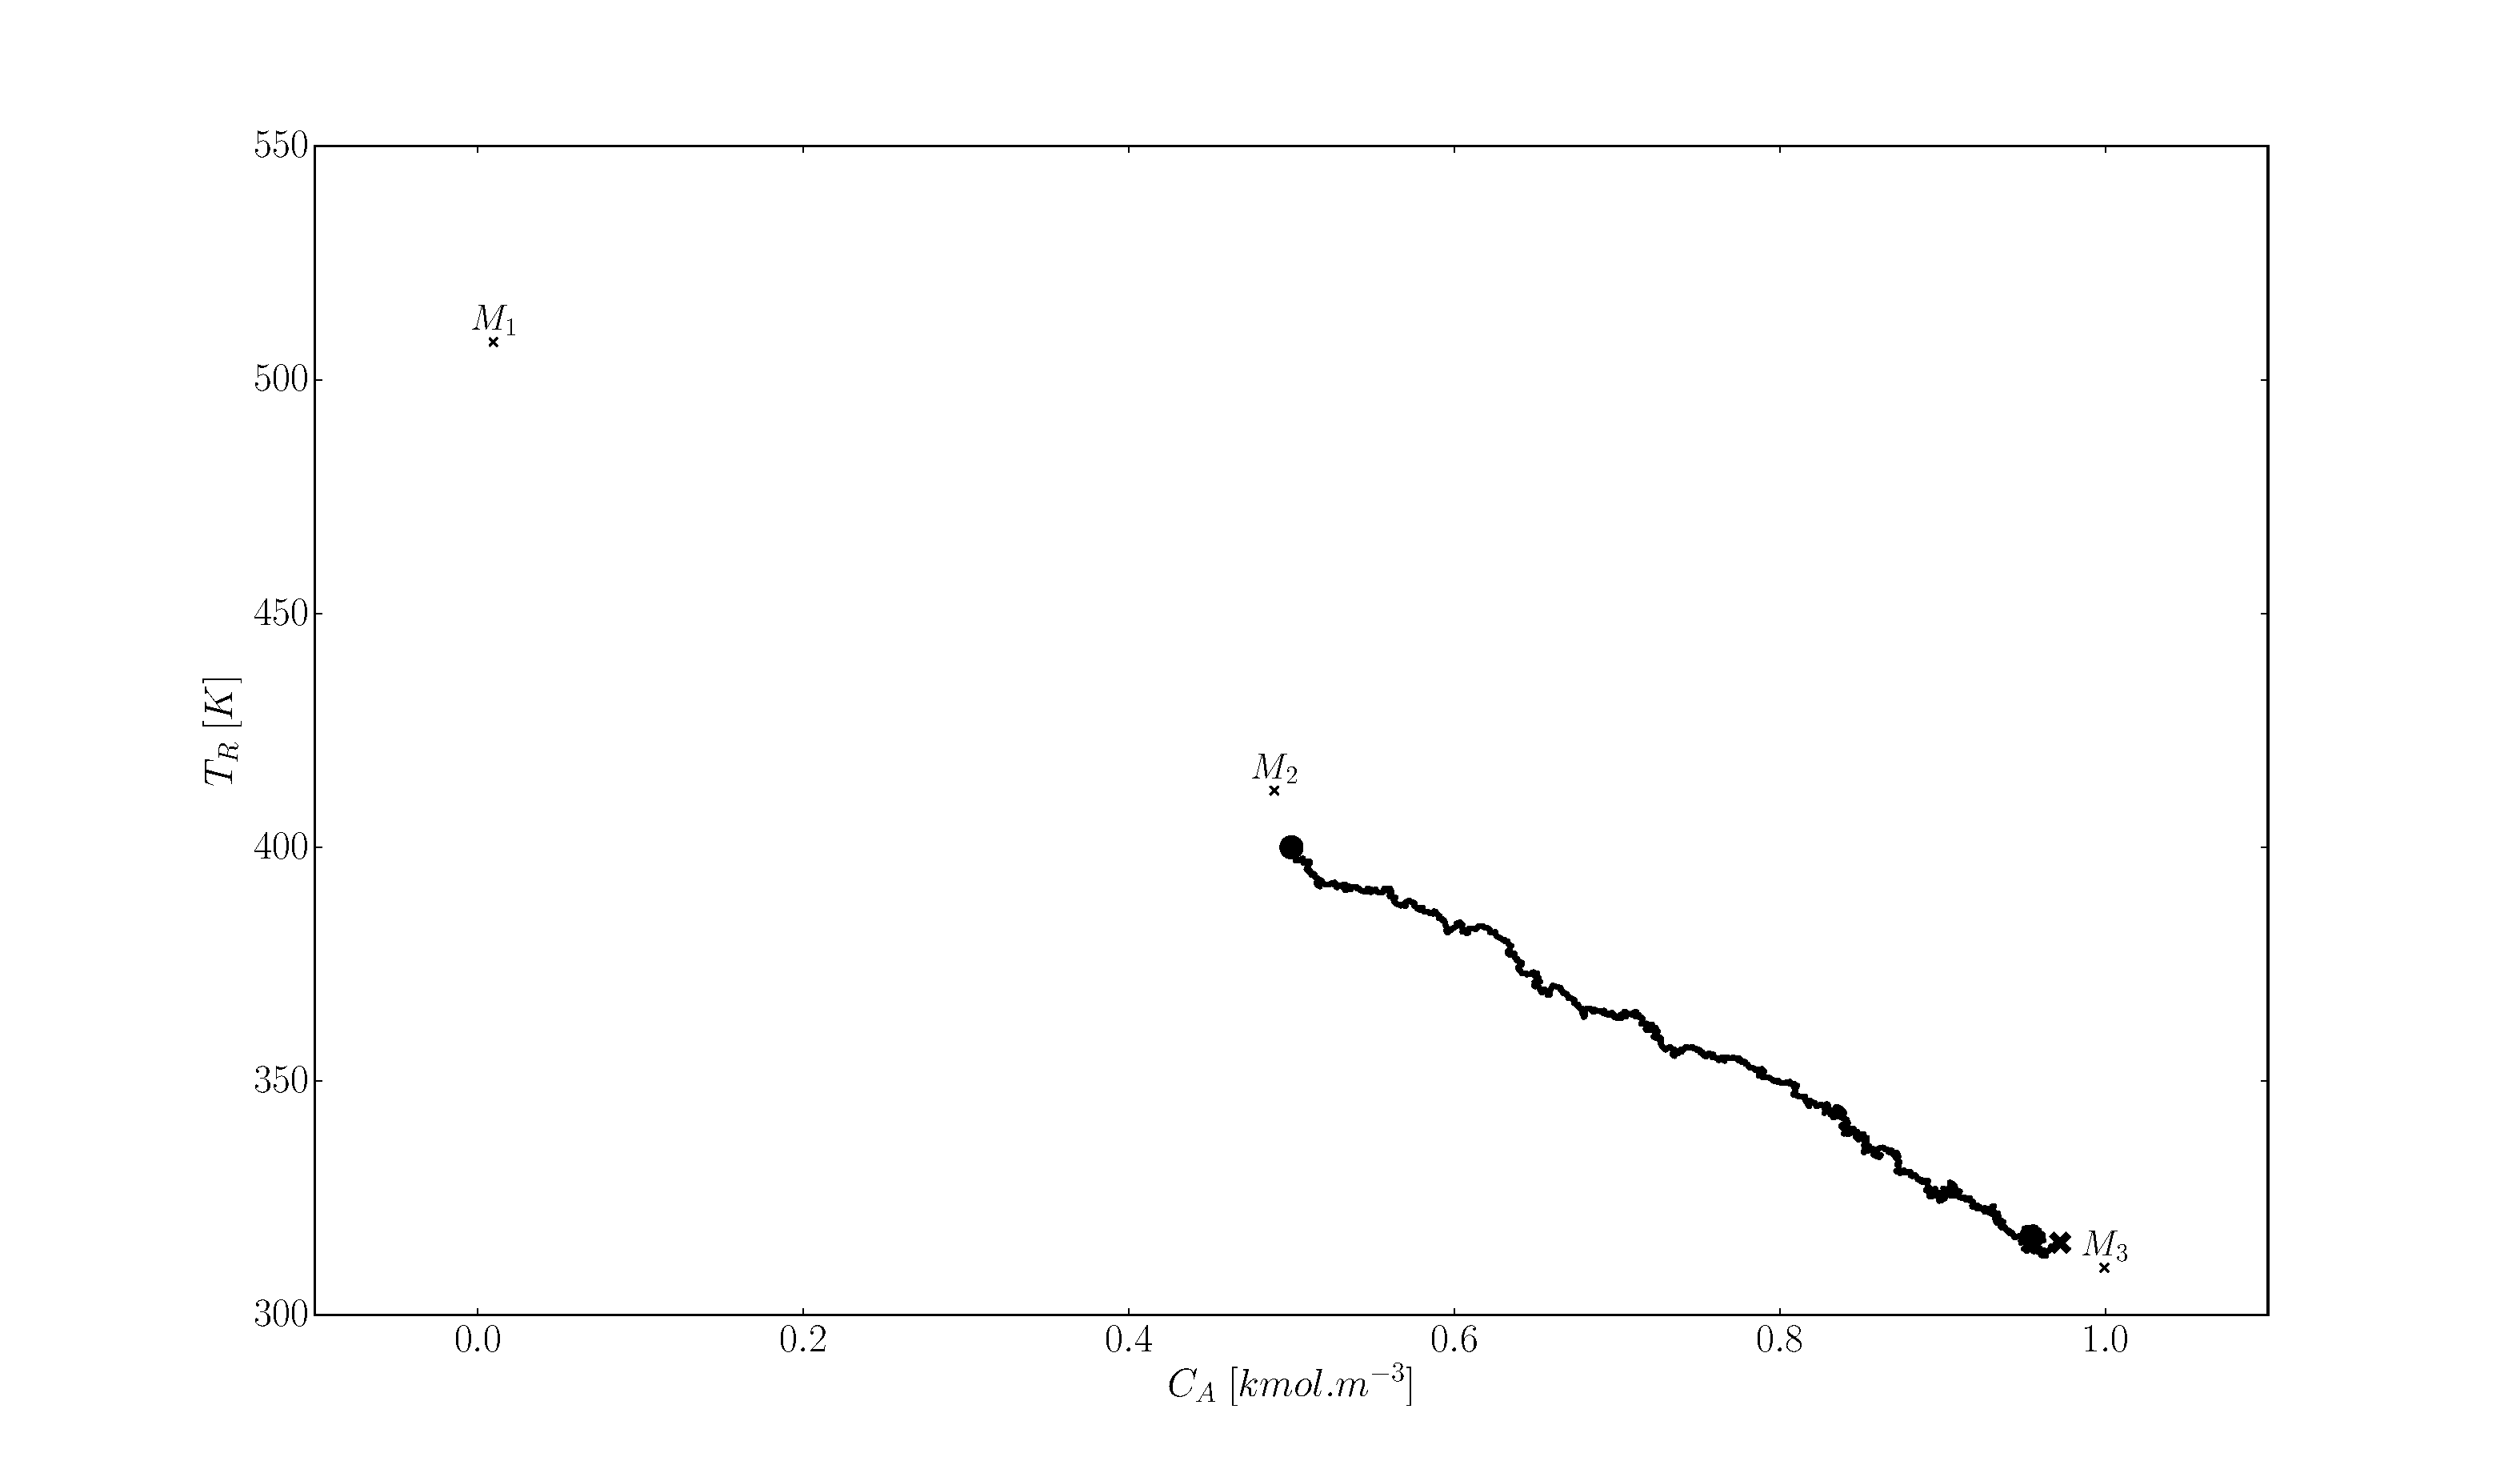
\includegraphics[scale=0.25]{rbpf_3m_models.pdf}
\caption{State space of the CSTR problem with the position of the 3 linear models superimposed thereupon. The trajectory followed by the system is also shown, the dot is the initial point and the cross the final point.}
\label{fig_3m_models}
\end{figure}
It is clear from Figure \ref{fig_3m_models} that we expect the filter to use $M_2$ initially and then switch to $M_3$ as time progresses. Figure \ref{fig_3m_vage_track} shows how the RBPF filters the CSTR over a simulation window of 150 minutes. The average concentration error is 21.95\% and the average temperature error is 0.42\% for the state estimator.
\begin{figure}[H] 
\centering
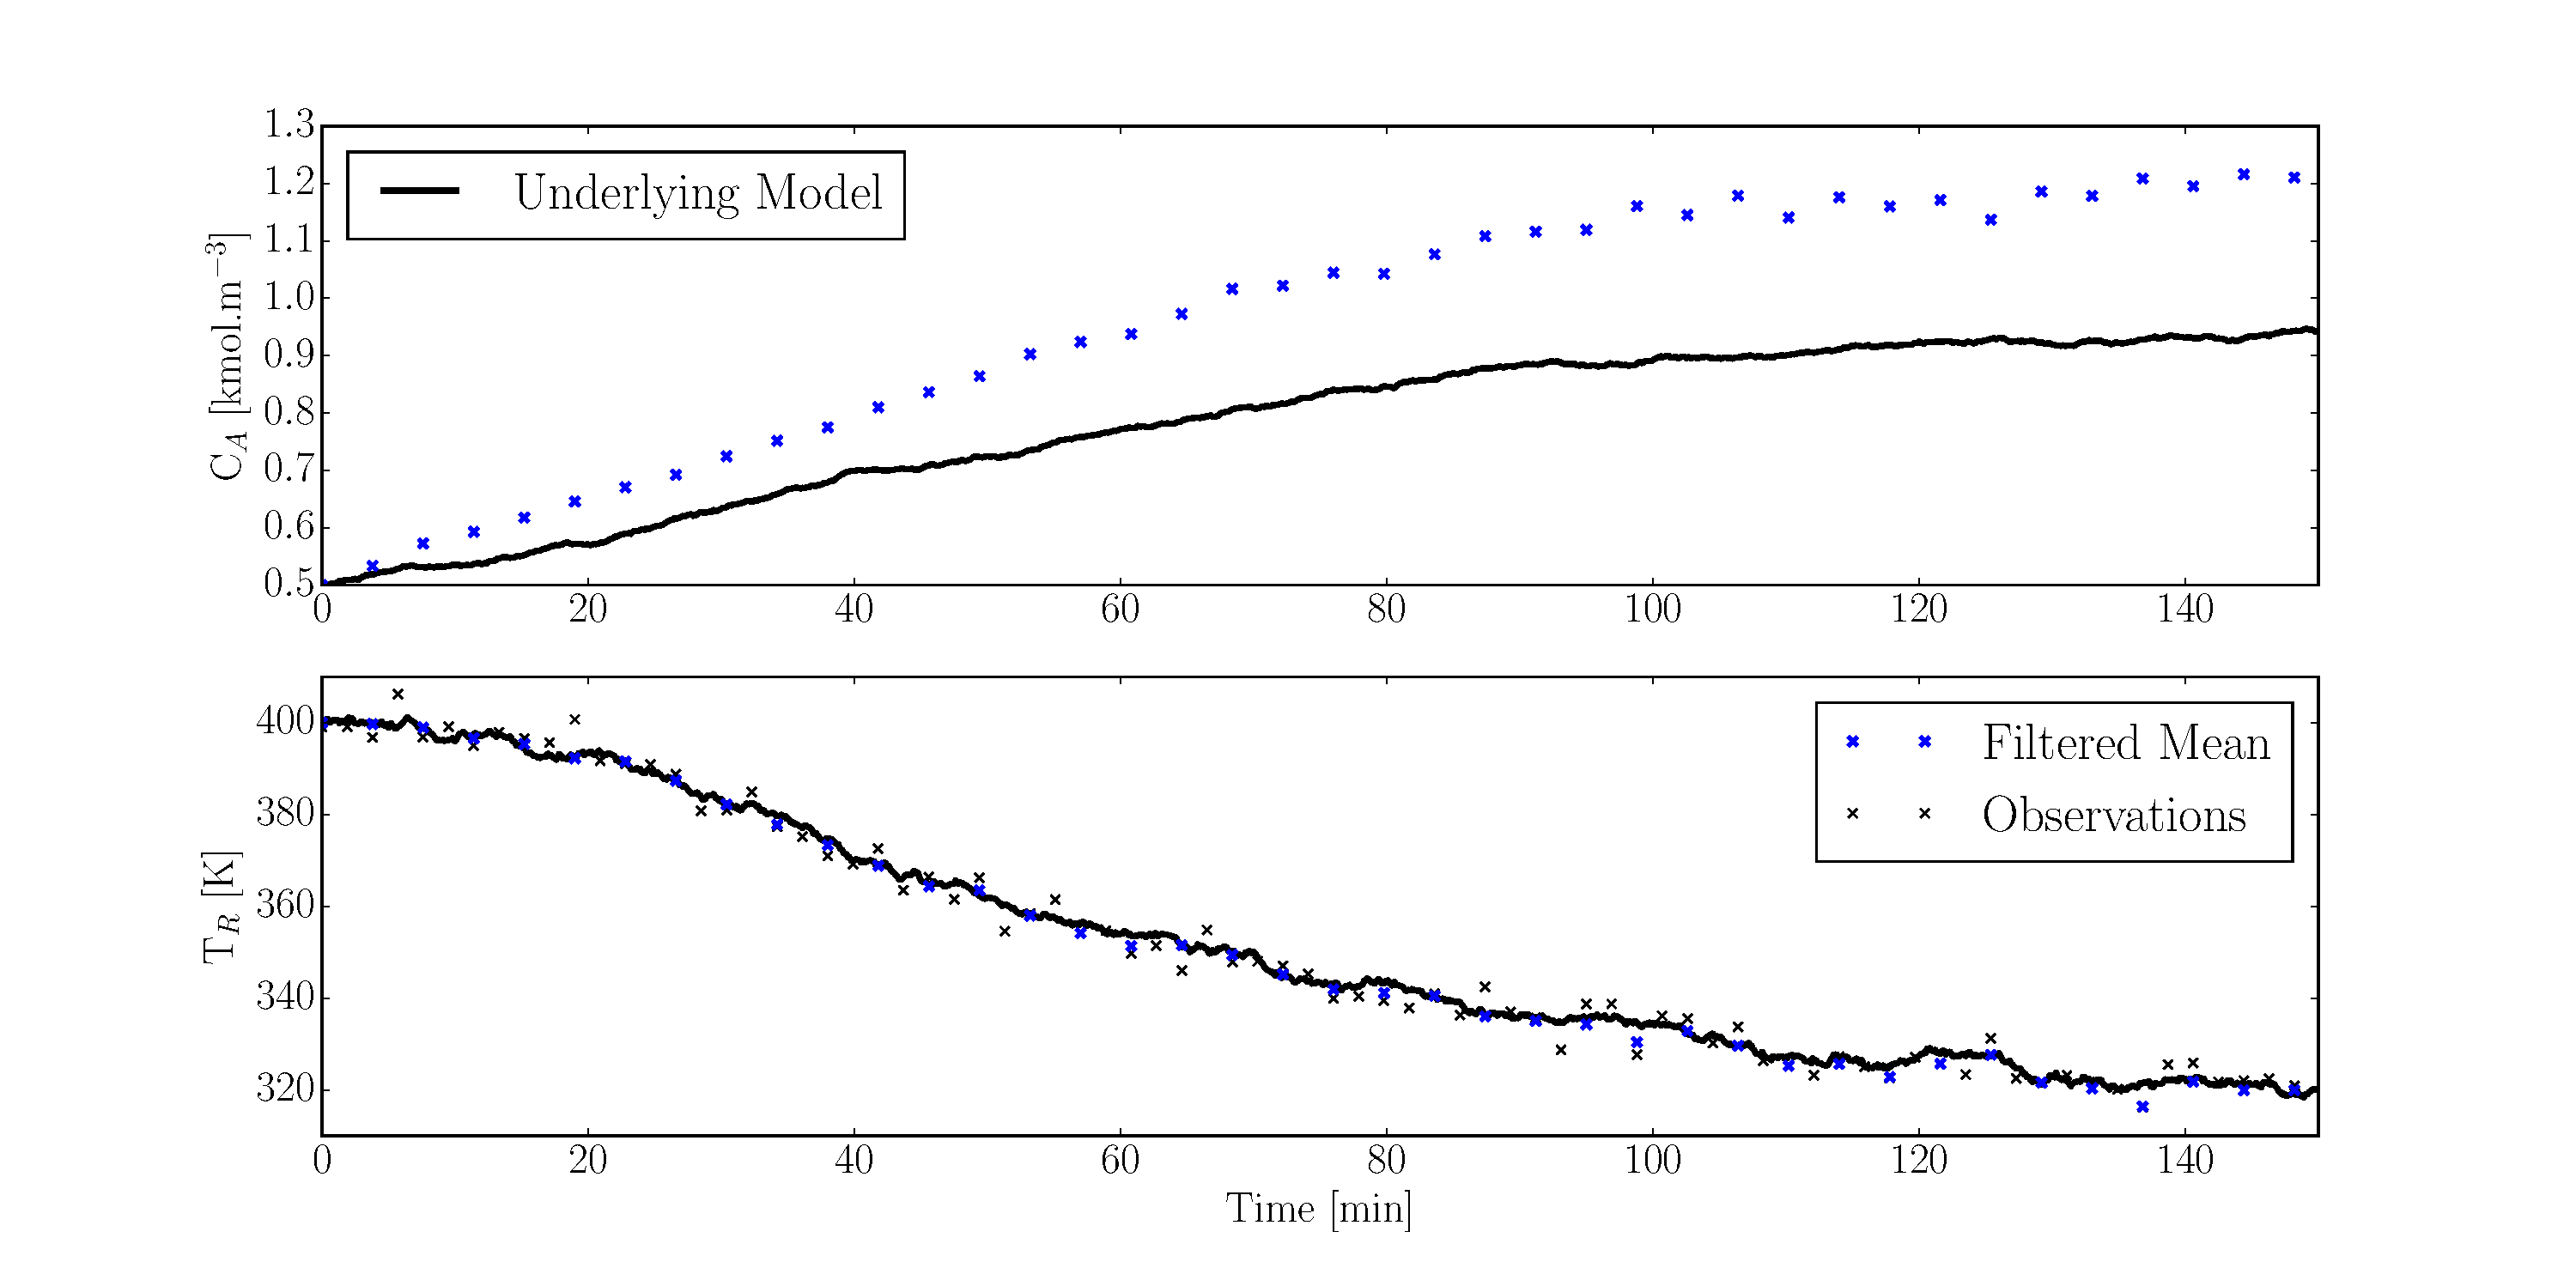
\includegraphics[scale=0.25]{rbpf_3m_vague_track.pdf}
\caption{Filtering with the RBPF using 3 linear models and 500 particles. Switch transition matrix $P_1$ was used.}
\label{fig_3m_vage_track}
\end{figure}
Figure \ref{fig_3m_vage_switch} shows the state of the corresponding switching variable $s_t$ over time. Since $s_t$ is a discrete random variable we have that at each time slice $\sum_{i=1}^{M=3} s_t^i = 1$.
\begin{figure}[H] 
\centering
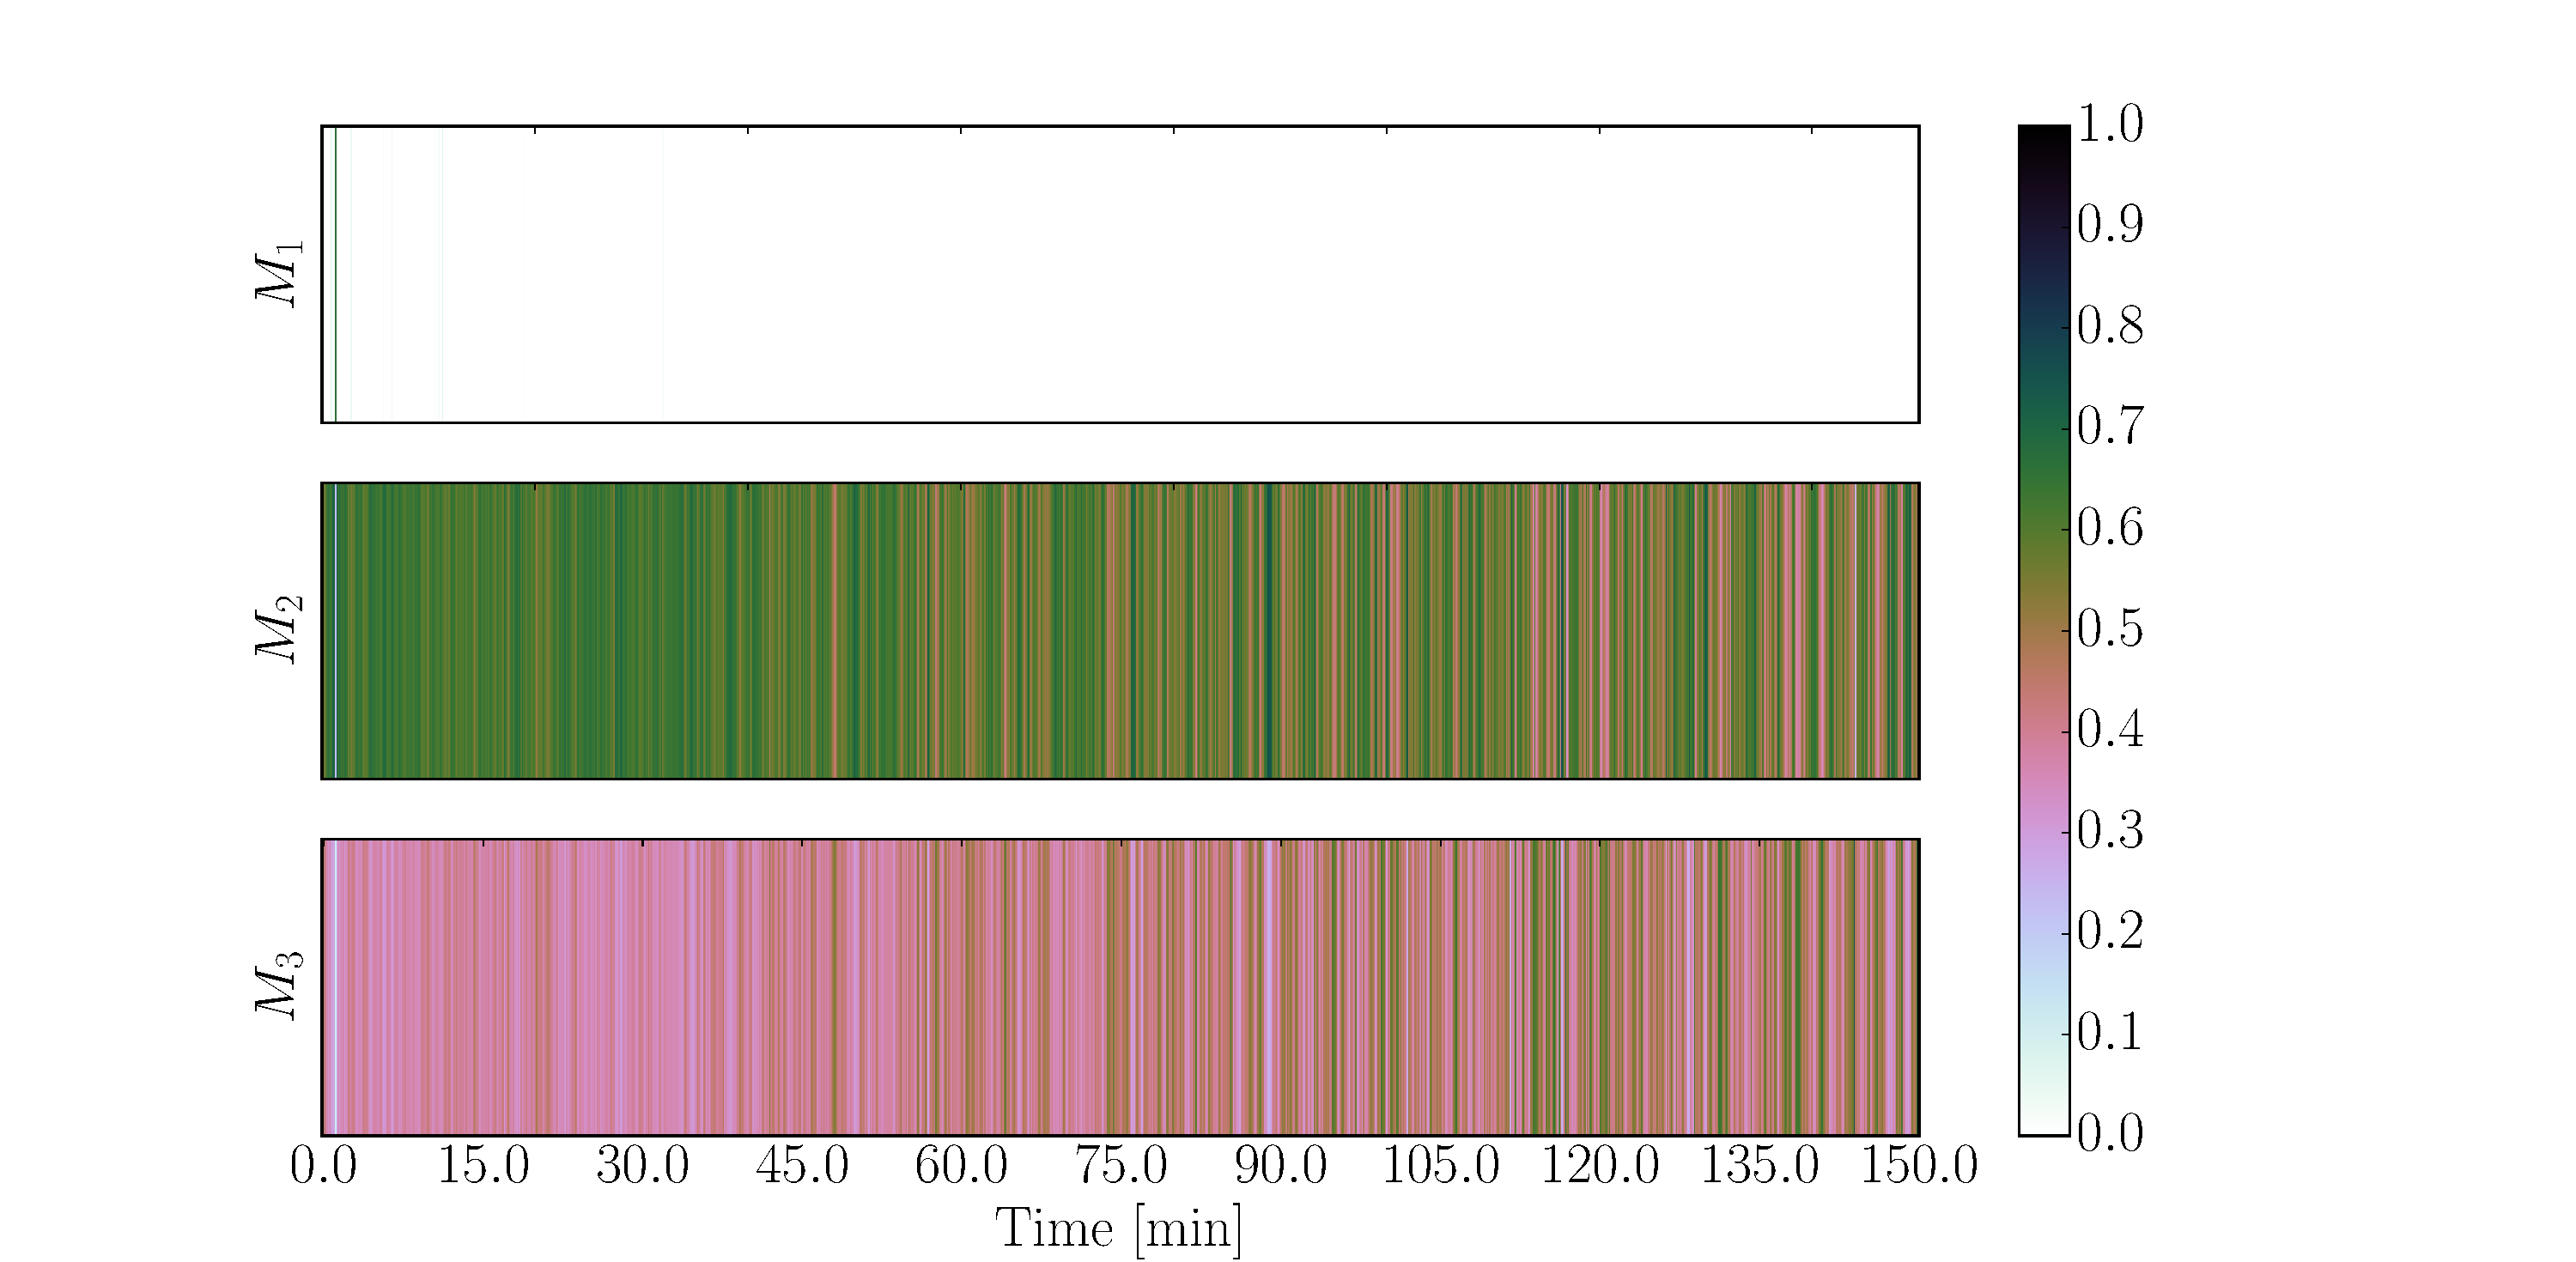
\includegraphics[scale=0.25]{rbpf_3m_vague_switch.pdf}
\caption{State of the switching variable $s_t$ over time. The weight indicates the sum of the particle weights per model.}
\label{fig_3m_vage_switch}
\end{figure}
From Figure \ref{fig_3m_vage_track} we see that the filtering error is quite large in the unmeasured state. This has been the trend when performing inference on an unmeasured state, however the magnitude of the error does not justify the use of the more complicated Graphical Model. Additionally, we see that there is no clear switching point in Figure \ref{fig_3m_vage_switch} - the filter relies on both $M_2$ an $M_3$ to estimate the state throughout the simulation. This is contrary to what we expected based on Figure \ref{fig_3m_models}.

Figure \ref{fig_3m_track} shows how the RBPF filters the CSTR over a simulation window of 150 minutes using $P_2$. The average concentration error is 5.05\% and the average temperature error is 0.33\% for the state estimator. This is a vast improvement over the case where $P_1$ was used.
\begin{figure}[H] 
\centering
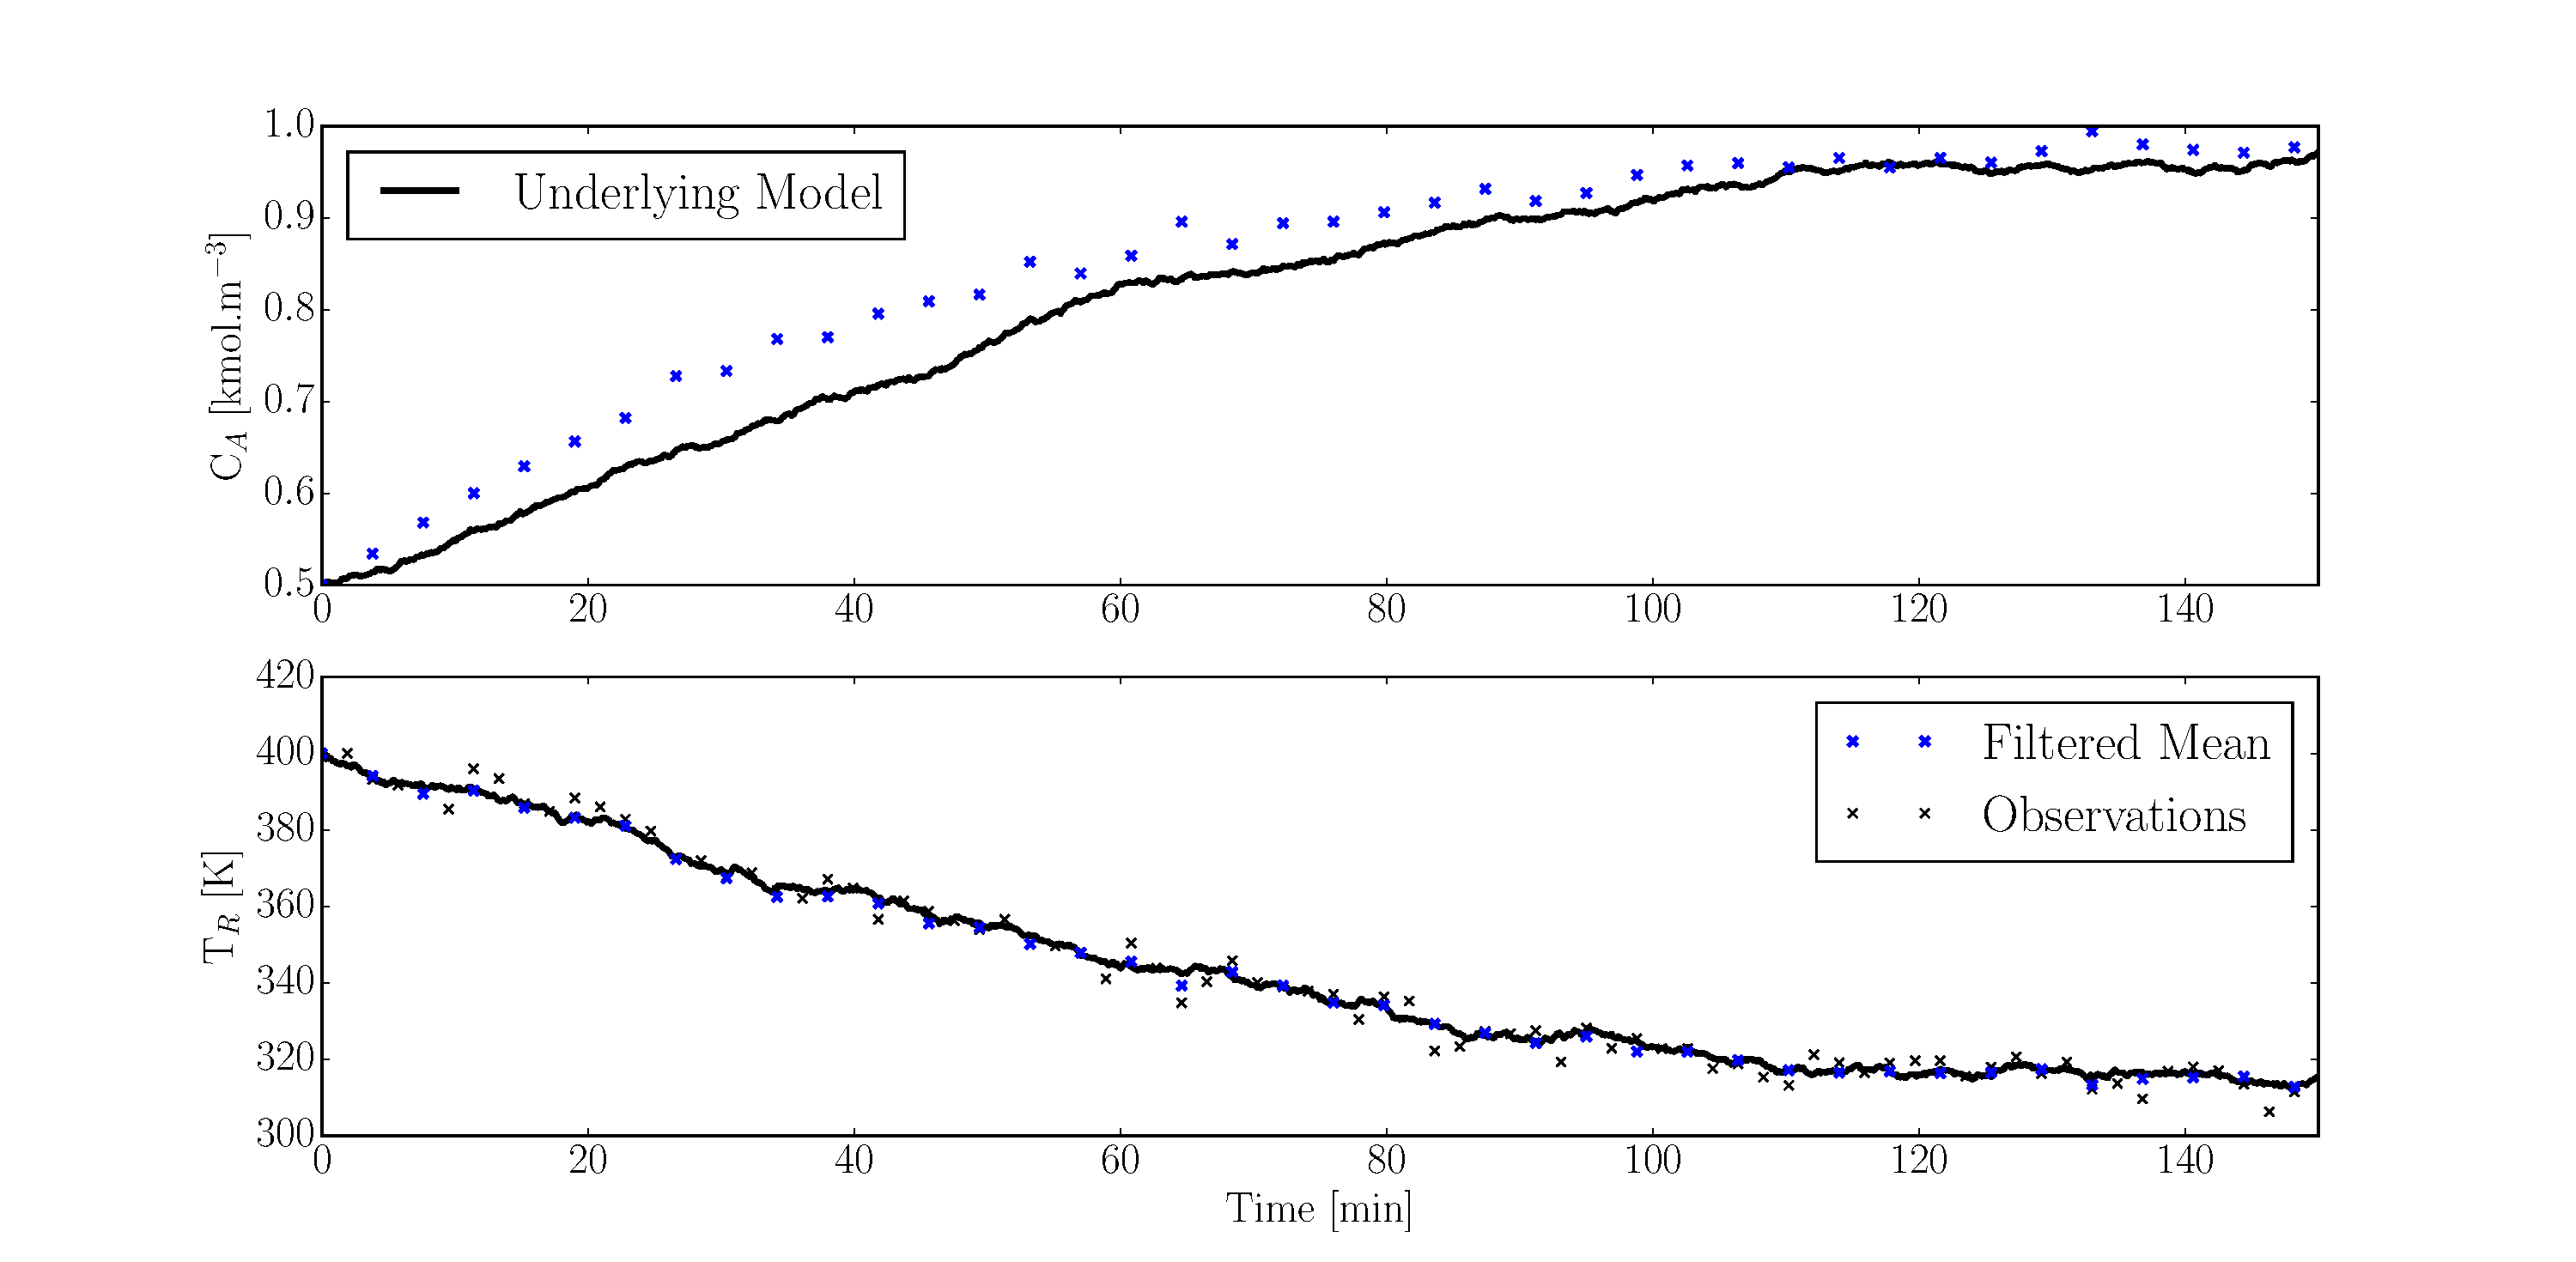
\includegraphics[scale=0.25]{rbpf_3m_track.pdf}
\caption{Filtering with the RBPF using 3 linear models and 500 particles. Switch transition matrix $P_2$ was used.}
\label{fig_3m_track}
\end{figure}
Figure \ref{fig_3m_switch} shows the state of the corresponding switching variable $s_t$ over time.
\begin{figure}[H] 
\centering
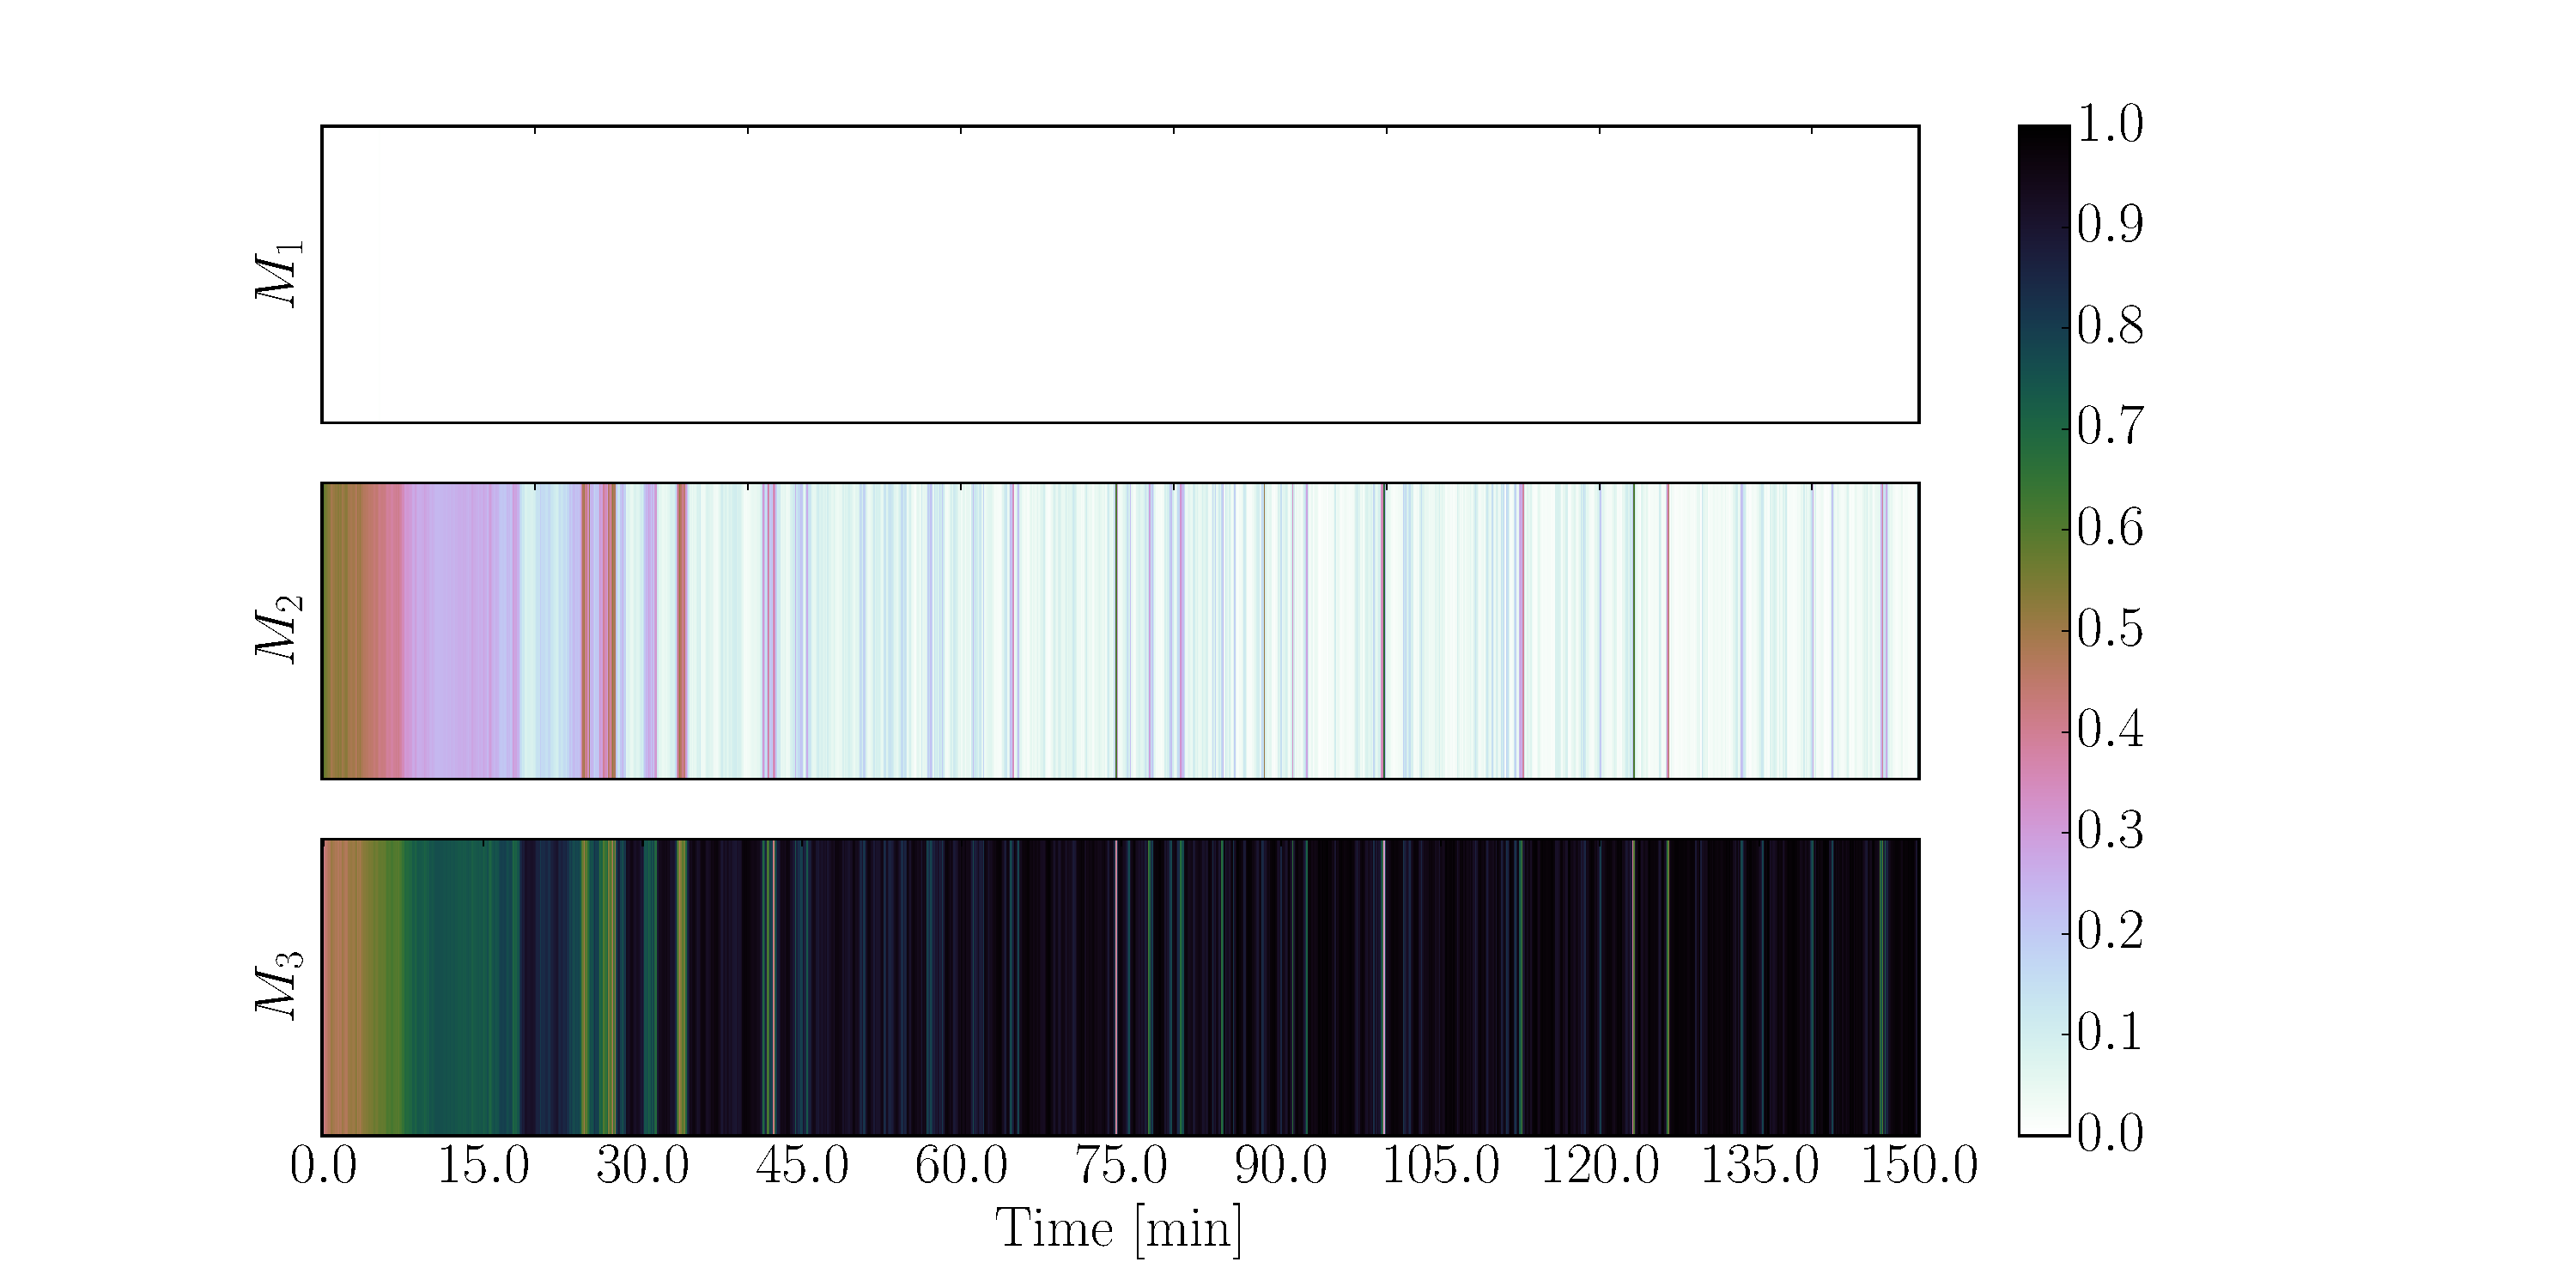
\includegraphics[scale=0.25]{rbpf_3m_switch.pdf}
\caption{State of the switching variable $s_t$ over time. The weight indicates the sum of the particle weights per model.}
\label{fig_3m_switch}
\end{figure}
Unlike Figure \ref{fig_3m_vage_switch} we do see a clear model transition around the 20 minute mark in Figure \ref{fig_3m_switch}. This is the behaviour we expected - as the system moves away from the unstable operating point the corresponding Graphical Model becomes less important.

These results suggest that the switch transition matrix sets how ``sticky" the model transitions are. The more vague they are, as in the case of $P_1$, the more unsure the filter is about which model is probably generating the observations. On the other hand, in the case of $P_2$, once the filter switched to the higher probability model it stayed there. This behaviour is desirable because it is easier to base a control strategy off of one model than multiple models. However, the immediate drawback of the ``sticky" approach is that the filter may be over confident. Additionally if a machine learning approach is not used to infer the values of $P$ it could become a tedious task to set $P$ for a large system. Clearly the values used in $P_2$ were set my hand - more investigation is necessary to determine proper heuristics if this approach should be adopted in practice.

Next we investigate the effect using more models has on the filter. We use the same 3 model filter as before (using $P_2$) but compare it to a 7 model filter. The state transition matrix for the 7 model filter is shown in (\ref{eq_state_trans7}).
\begin{equation}
P_3 = \begin{pmatrix}
0.98 & 0.00 & 0.00 & 0.00 & 0.00 & 0.01 & 0.00 \\
0.00 & 0.98 & 0.00 & 0.01 & 0.01 & 0.01 & 0.00 \\
0.01 & 0.00 & 0.98 & 0.00 & 0.00 & 0.01 & 0.01 \\
0.00 & 0.00 & 0.00 & 0.98 & 0.00 & 0.01 & 0.00 \\
0.00 & 0.01 & 0.00 & 0.00 & 0.99 & 0.00 & 0.00 \\
0.01 & 0.01 & 0.01 & 0.01 & 0.00 & 0.96 & 0.00 \\
0.00 & 0.00 & 0.01 & 0.00 & 0.00 & 0.00 & 0.99 \\
\end{pmatrix}
\label{eq_state_trans7}
\end{equation}
The values of $P_3$ were set using the same reasoning as before. Figure \ref{fig_7m_models} show state trajectory of the system (like Figure \ref{fig_3m_models}) but with the additional models superimposed thereupon. Clearly $M_5$, $M_6$ and $M_7$ correspond to high temperature, unstable and low temperature operating points. 
\begin{figure}[H] 
\centering
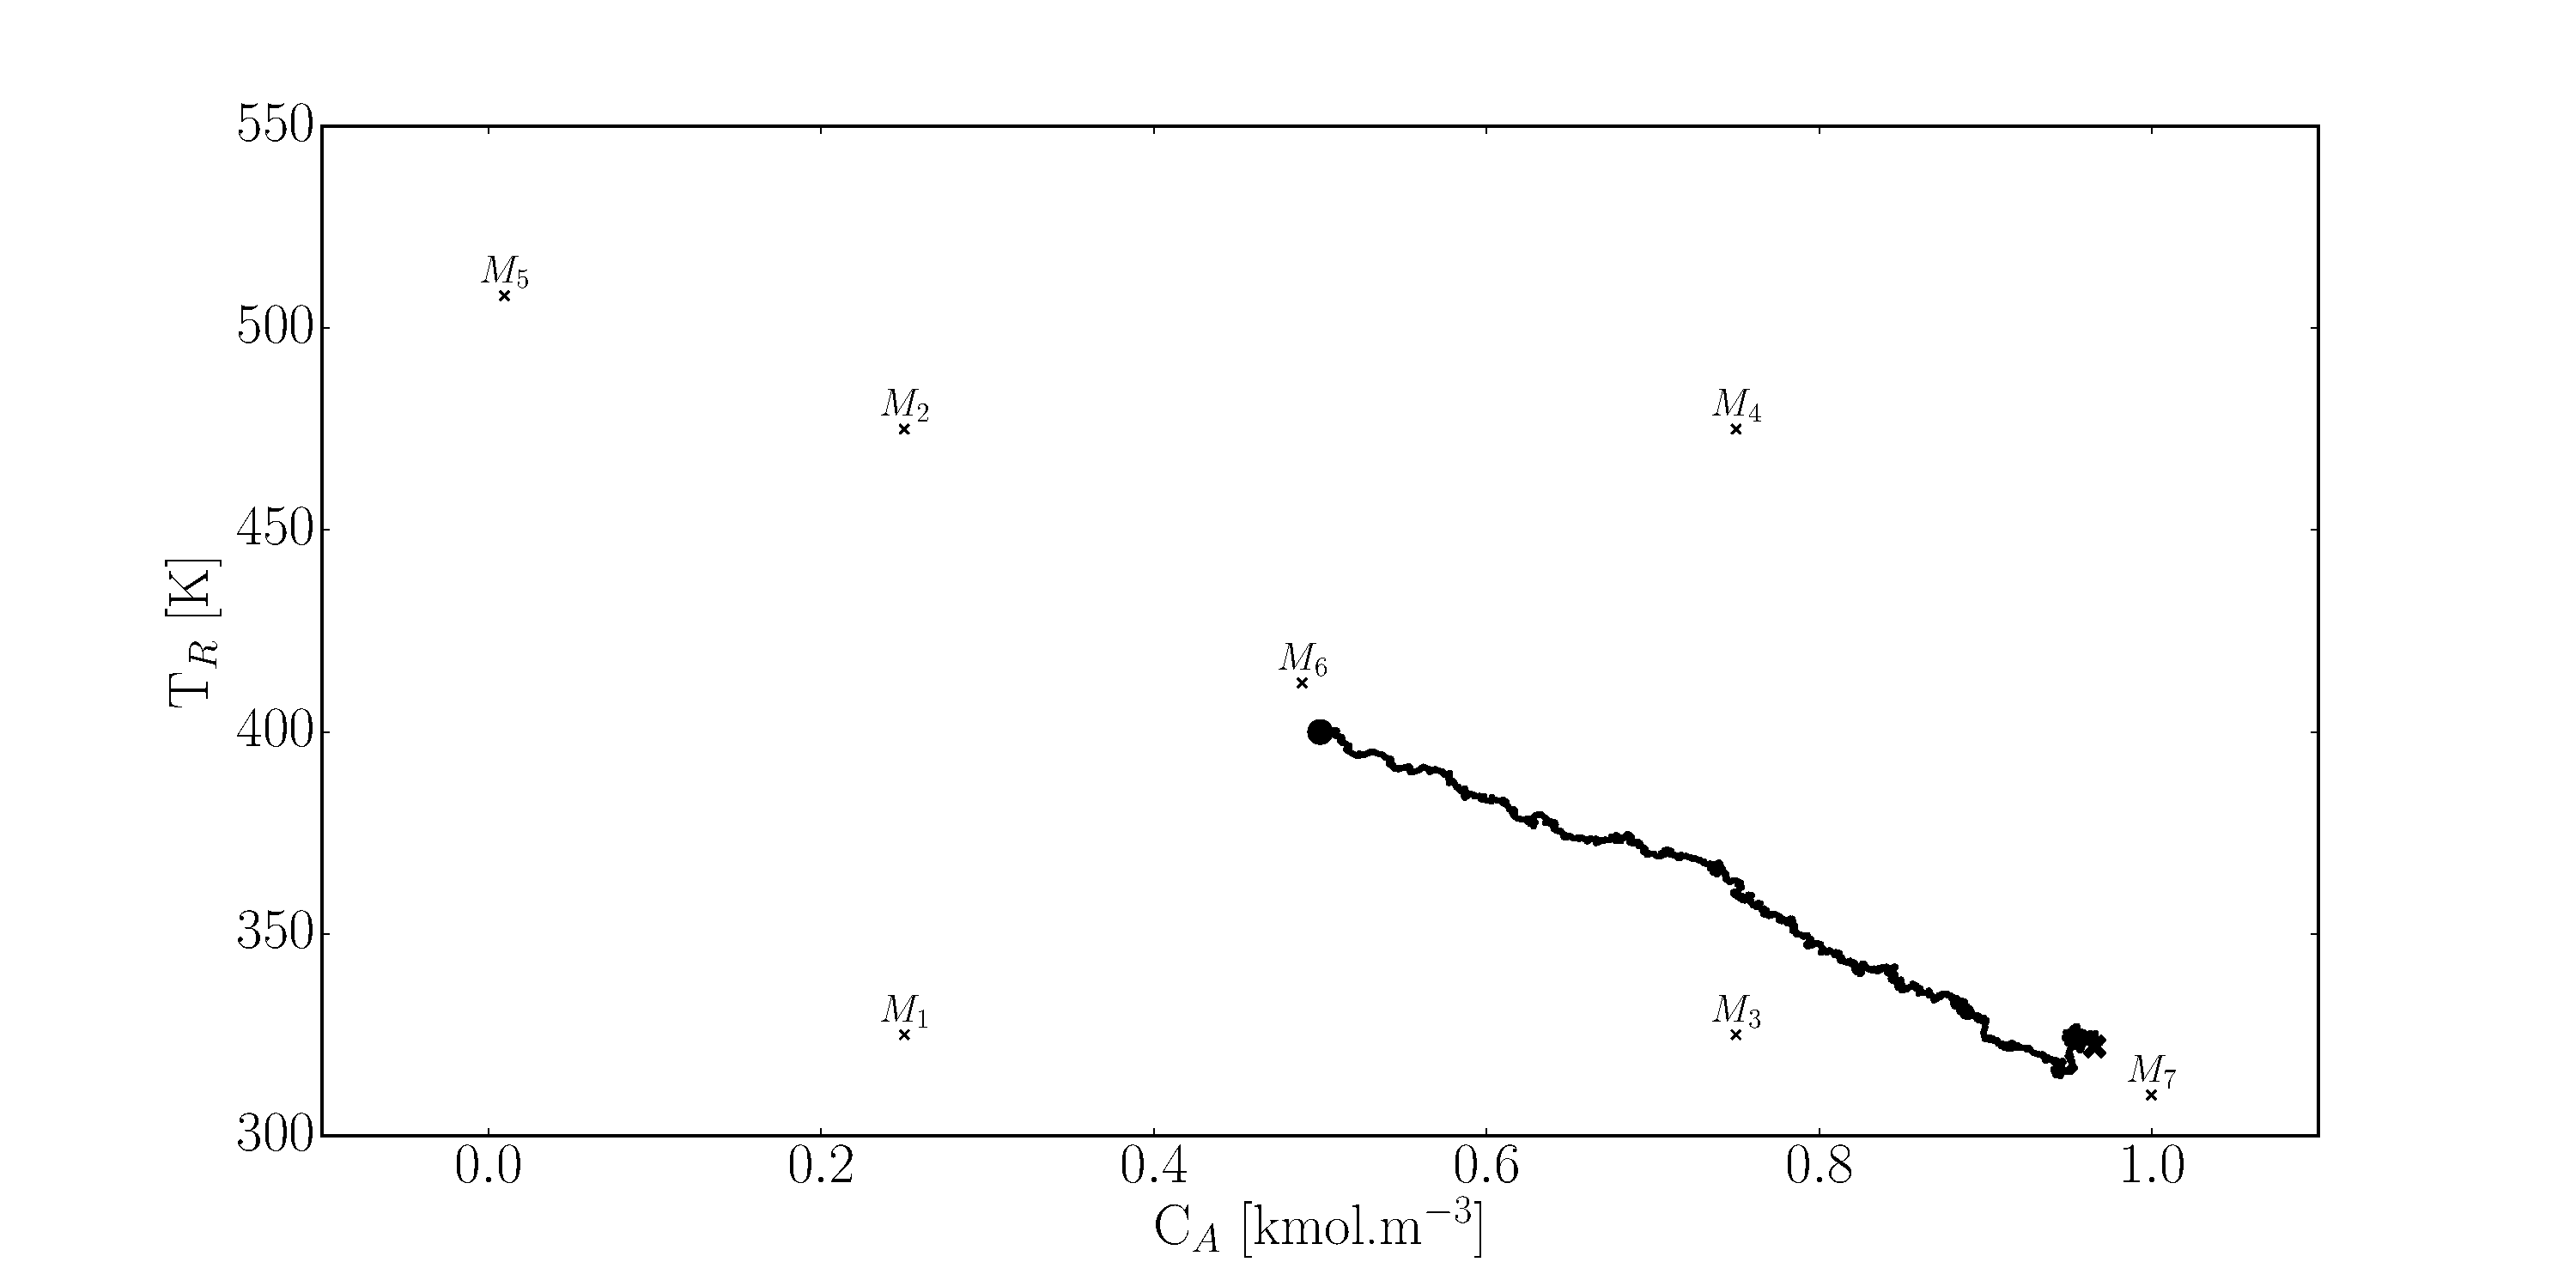
\includegraphics[scale=0.25]{rbpf_7m_models.pdf}
\caption{State space of the CSTR problem with the position of the 3 linear models superimposed thereupon. The trajectory followed by the system is also shown, the dot is the initial point and the cross the final point.}
\label{fig_7m_models}
\end{figure}
Figure \ref{fig_7m_track} shows the effectiveness of the filter over the simulation window. The average concentration and temperature error is 5.36\% and 0.36\% respectively. 
\begin{figure}[H] 
\centering
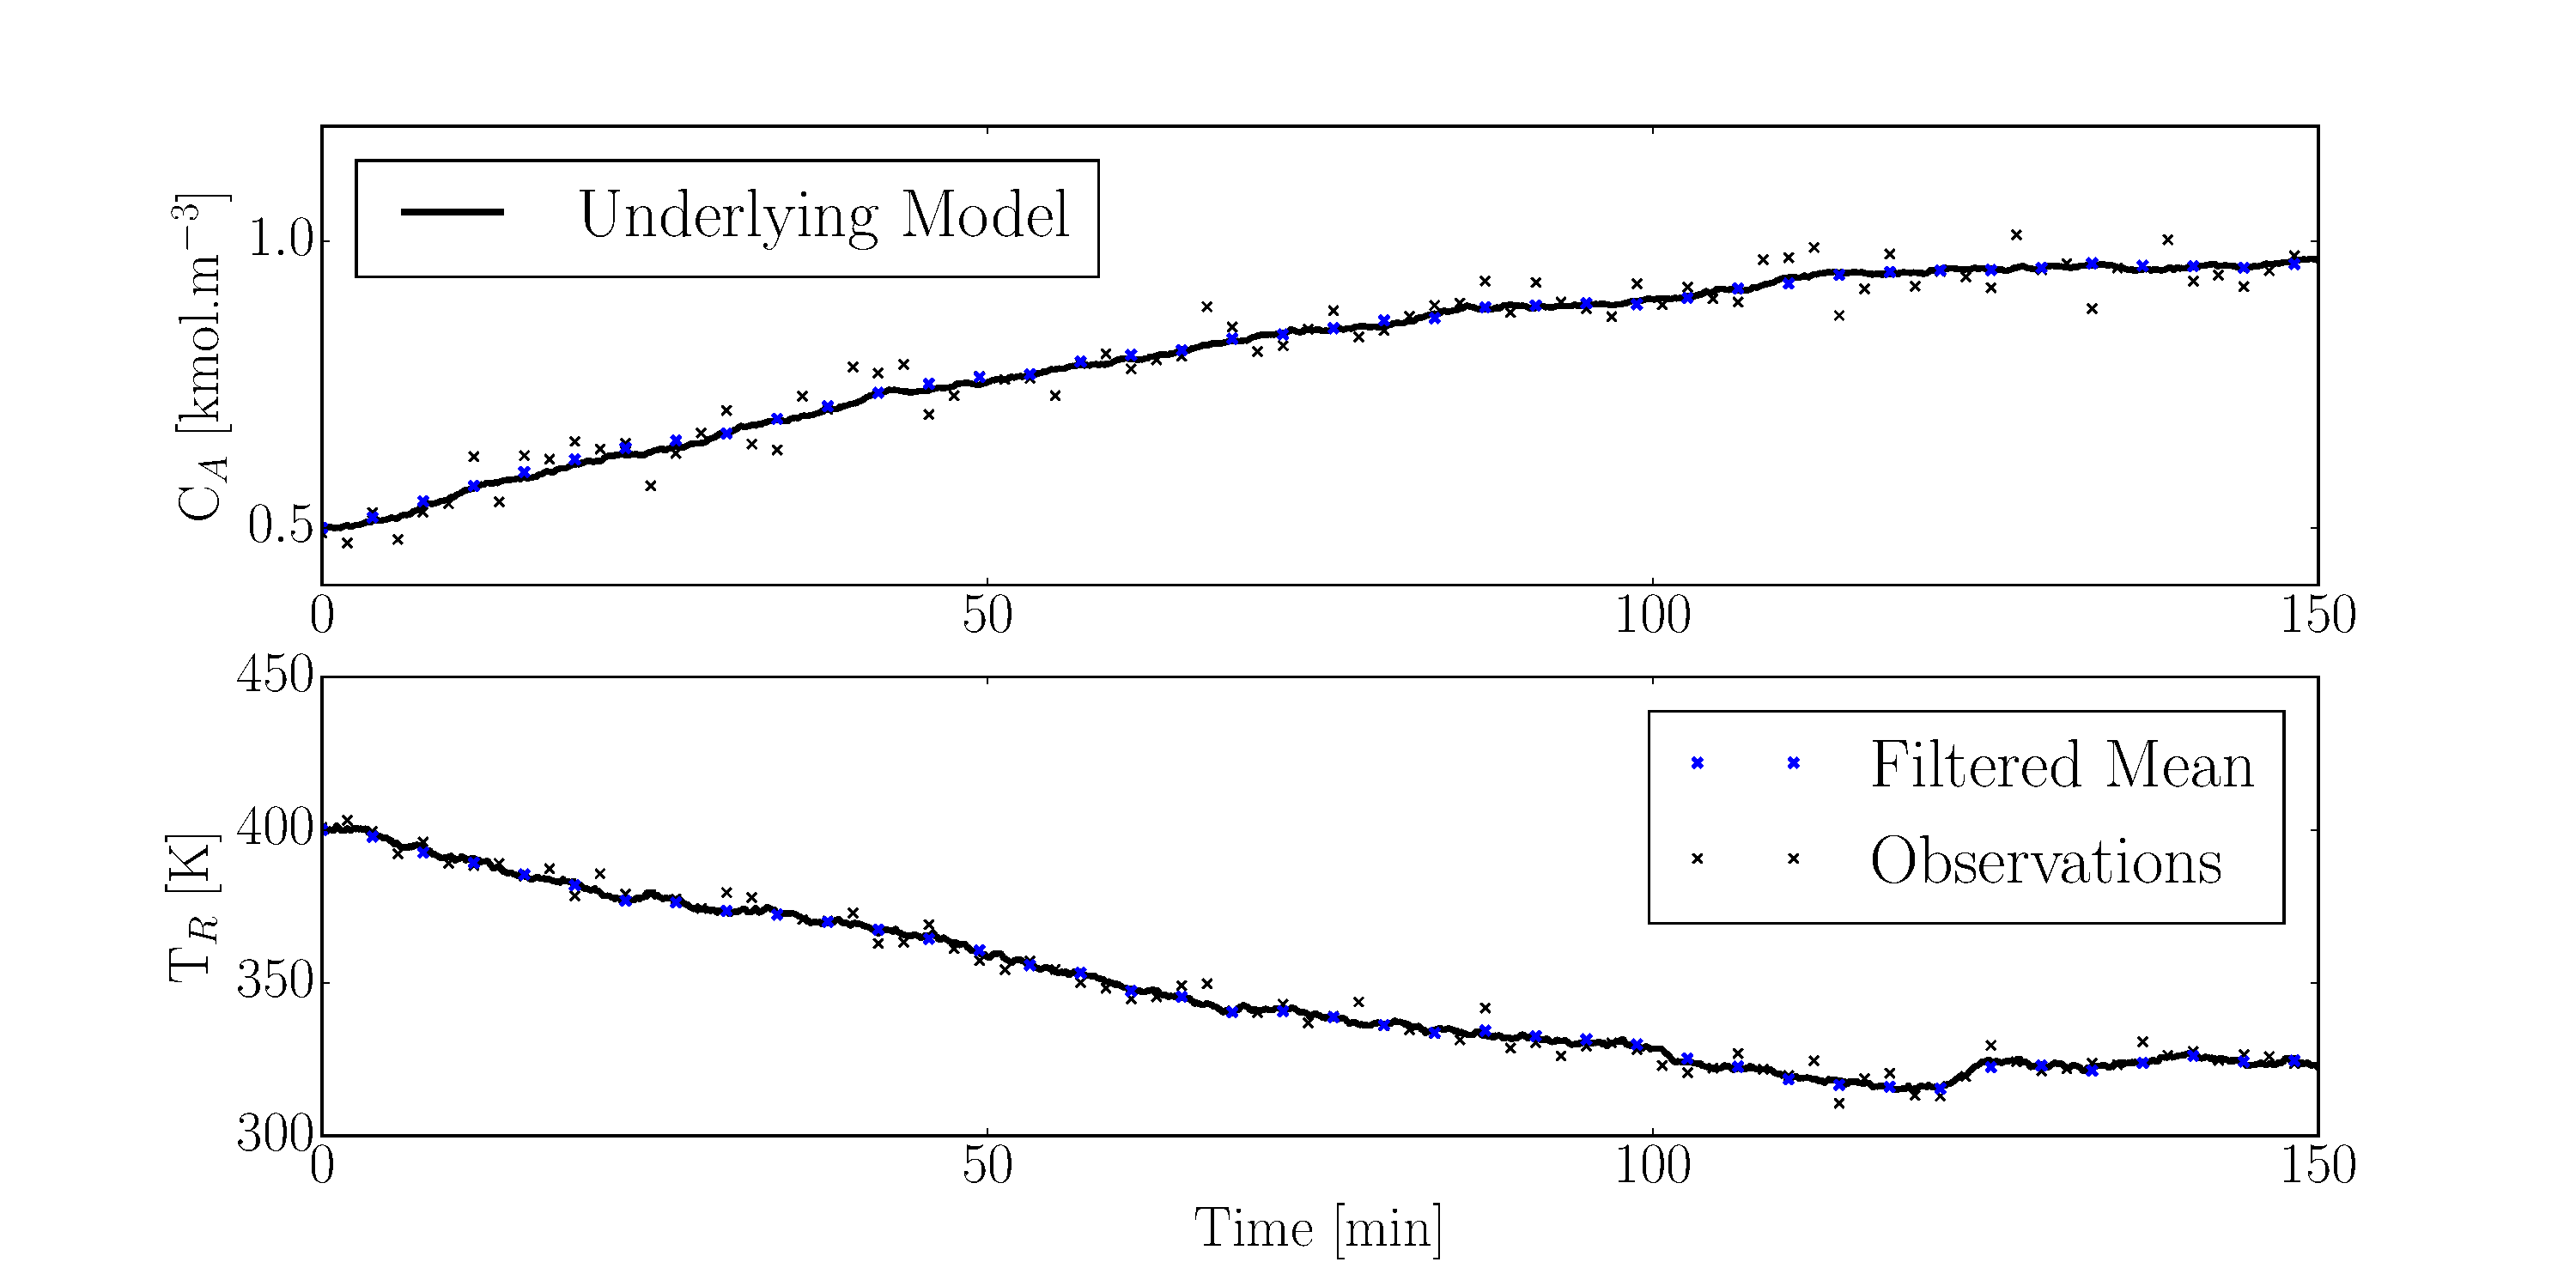
\includegraphics[scale=0.25]{rbpf_7m_track.pdf}
\caption{Filtering with the RBPF using 7 linear models and 500 particles. Switch transition matrix $P_3$ was used.}
\label{fig_7m_track}
\end{figure}
Interestingly enough we actually observe worse tracking performance when more models are used compared to the 3 model case with $P_2$. We expected the additional models to increase the effectiveness of the filter. Figure \ref{fig_7m_switch} shows the state of the corresponding switching variable $s_t$ over time. A possible explanation for the performance degradation is evident here.
\begin{figure}[H] 
\centering
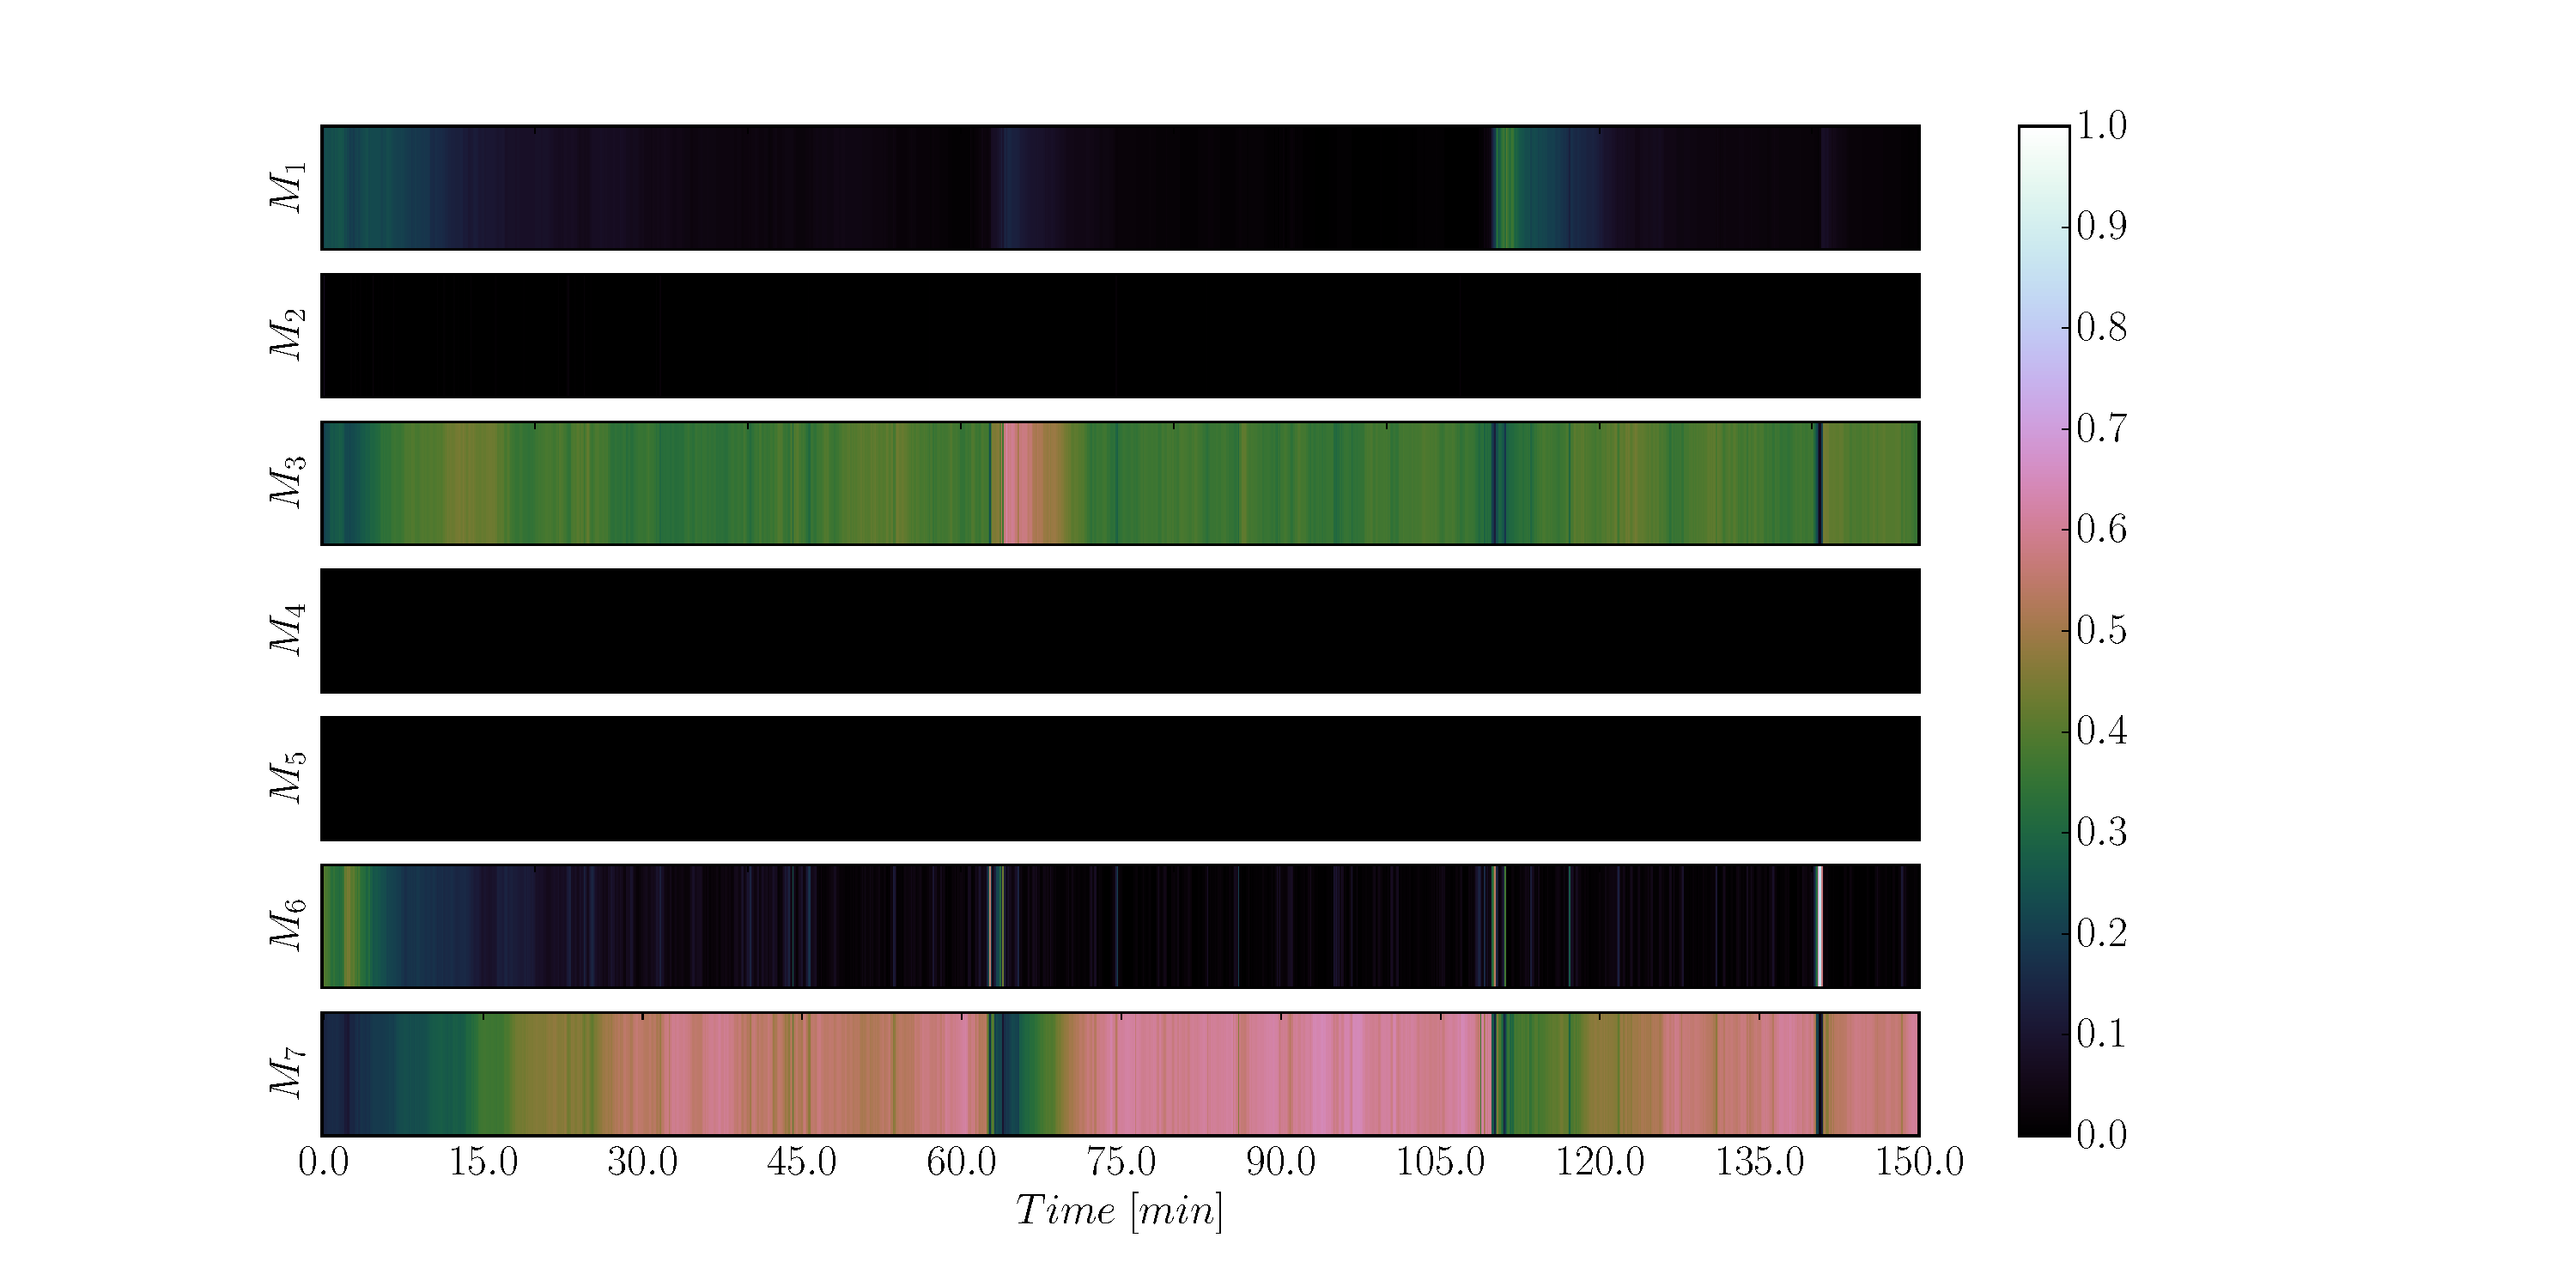
\includegraphics[scale=0.25]{rbpf_7m_switch.pdf}
\caption{State of the switching variable $s_t$ over time. The weight indicates the sum of the particle weights per model.}
\label{fig_7m_switch}
\end{figure}
We certainly expected $M_7$ to be the dominant model near the end of the simulation; however $M_3$, while close to the low temperature operating point, played a significant role in the state estimate throughout the simulation. While we only used the most likely model (clearly a particle using $M_7$) to estimate the current state it is evident that there were a non-negligible number of particles which maintained the $M_3$ hypothesis. This implies that less particles were available to use the $M_7$ model and thus we see worse performance.

The crux of the problem is model overlap. While it is clear to a human that the system should only use $M_7$ near the end of the simulation the algorithm has no way of knowing this. It infers this based on the predictive ability of the models. Clearly $M_7$, $M_3$ and to a lesser extent $M_1$ and $M_6$ were all able to accurately predict future behaviour. For this reason they have non-negligible weights in Figure \ref{fig_7m_switch}. 

We have in fact already come across this problem in Figures \ref{fig_3m_vage_track} and \ref{fig_3m_vage_switch}. We saw that it is possible to attenuate this problem by making the switching transition matrix more ``sticky". Unfortunately this does not solve the underlying problem - the models are not different enough. Using more models would only make this problem worse.

Finally we investigate the effect of measuring both states has on the accuracy of the filter. Due to the work in Sections \ref{sec_inf_lin_mods} and \ref{sec_inf_nonlin_mods} we expect that by measuring concentration we will increase the filter accuracy. We use the 3 model filter with $P_2$ to demonstrate that this is the case.

In Figure \ref{fig_3m_track_m2} we see the filtering performance of the RBPF measuring both states. The average concentration and temperature error is 0.88\% and 0.31\%. This is a significant improvement over the tracking we saw in Figure \ref{fig_3m_track}.
\begin{figure}[H] 
\centering
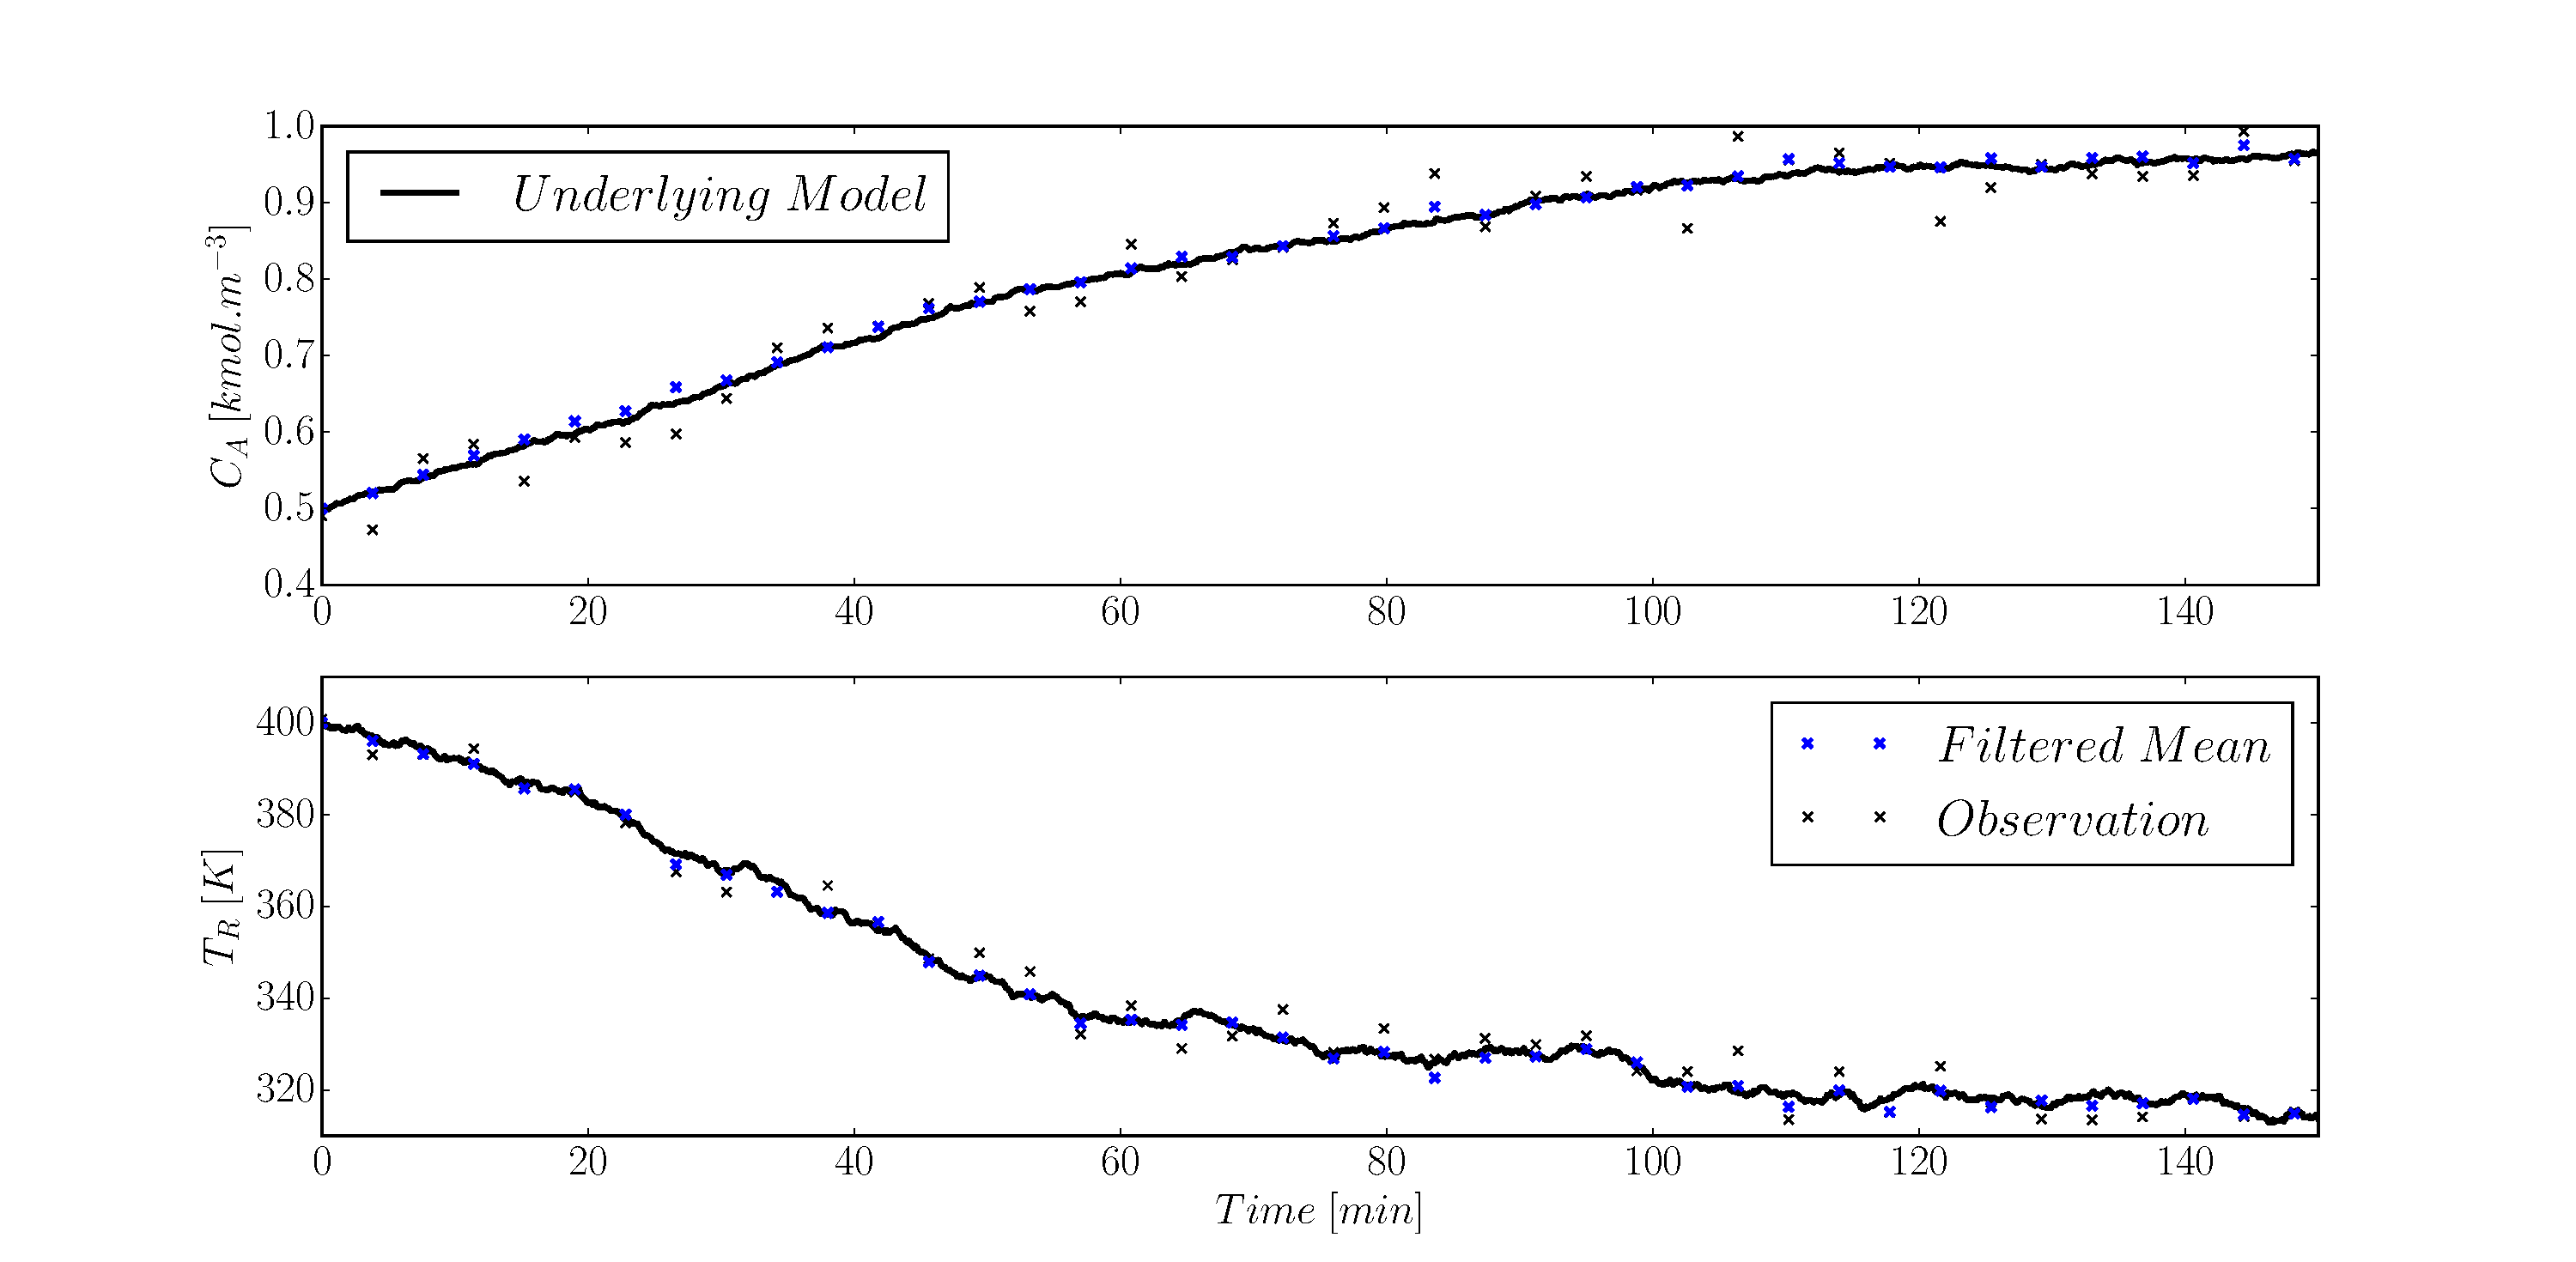
\includegraphics[scale=0.25]{rbpf_3m_track_m2.pdf}
\caption{Filtering with the RBPF using 3 linear models and 500 particles. Switch transition matrix $P_3$ was used.}
\label{fig_3m_track_m2}
\end{figure}
In Figure \ref{fig_3m_switch_m2} we see the state of the switching variable over the simulation run. Like Figure \ref{fig_3m_switch} we also see a clear switch occurring at approximately 15 minutes (actually at 20 minutes when measuring only one state). However, comparing Figures \ref{fig_3m_switch} and \ref{fig_3m_switch_m2} closely we see less ``switching noise" in the latter. The second measurement allows the filter to compare two state predictions to discern between models. This is clearly beneficial.
\begin{figure}[H] 
\centering
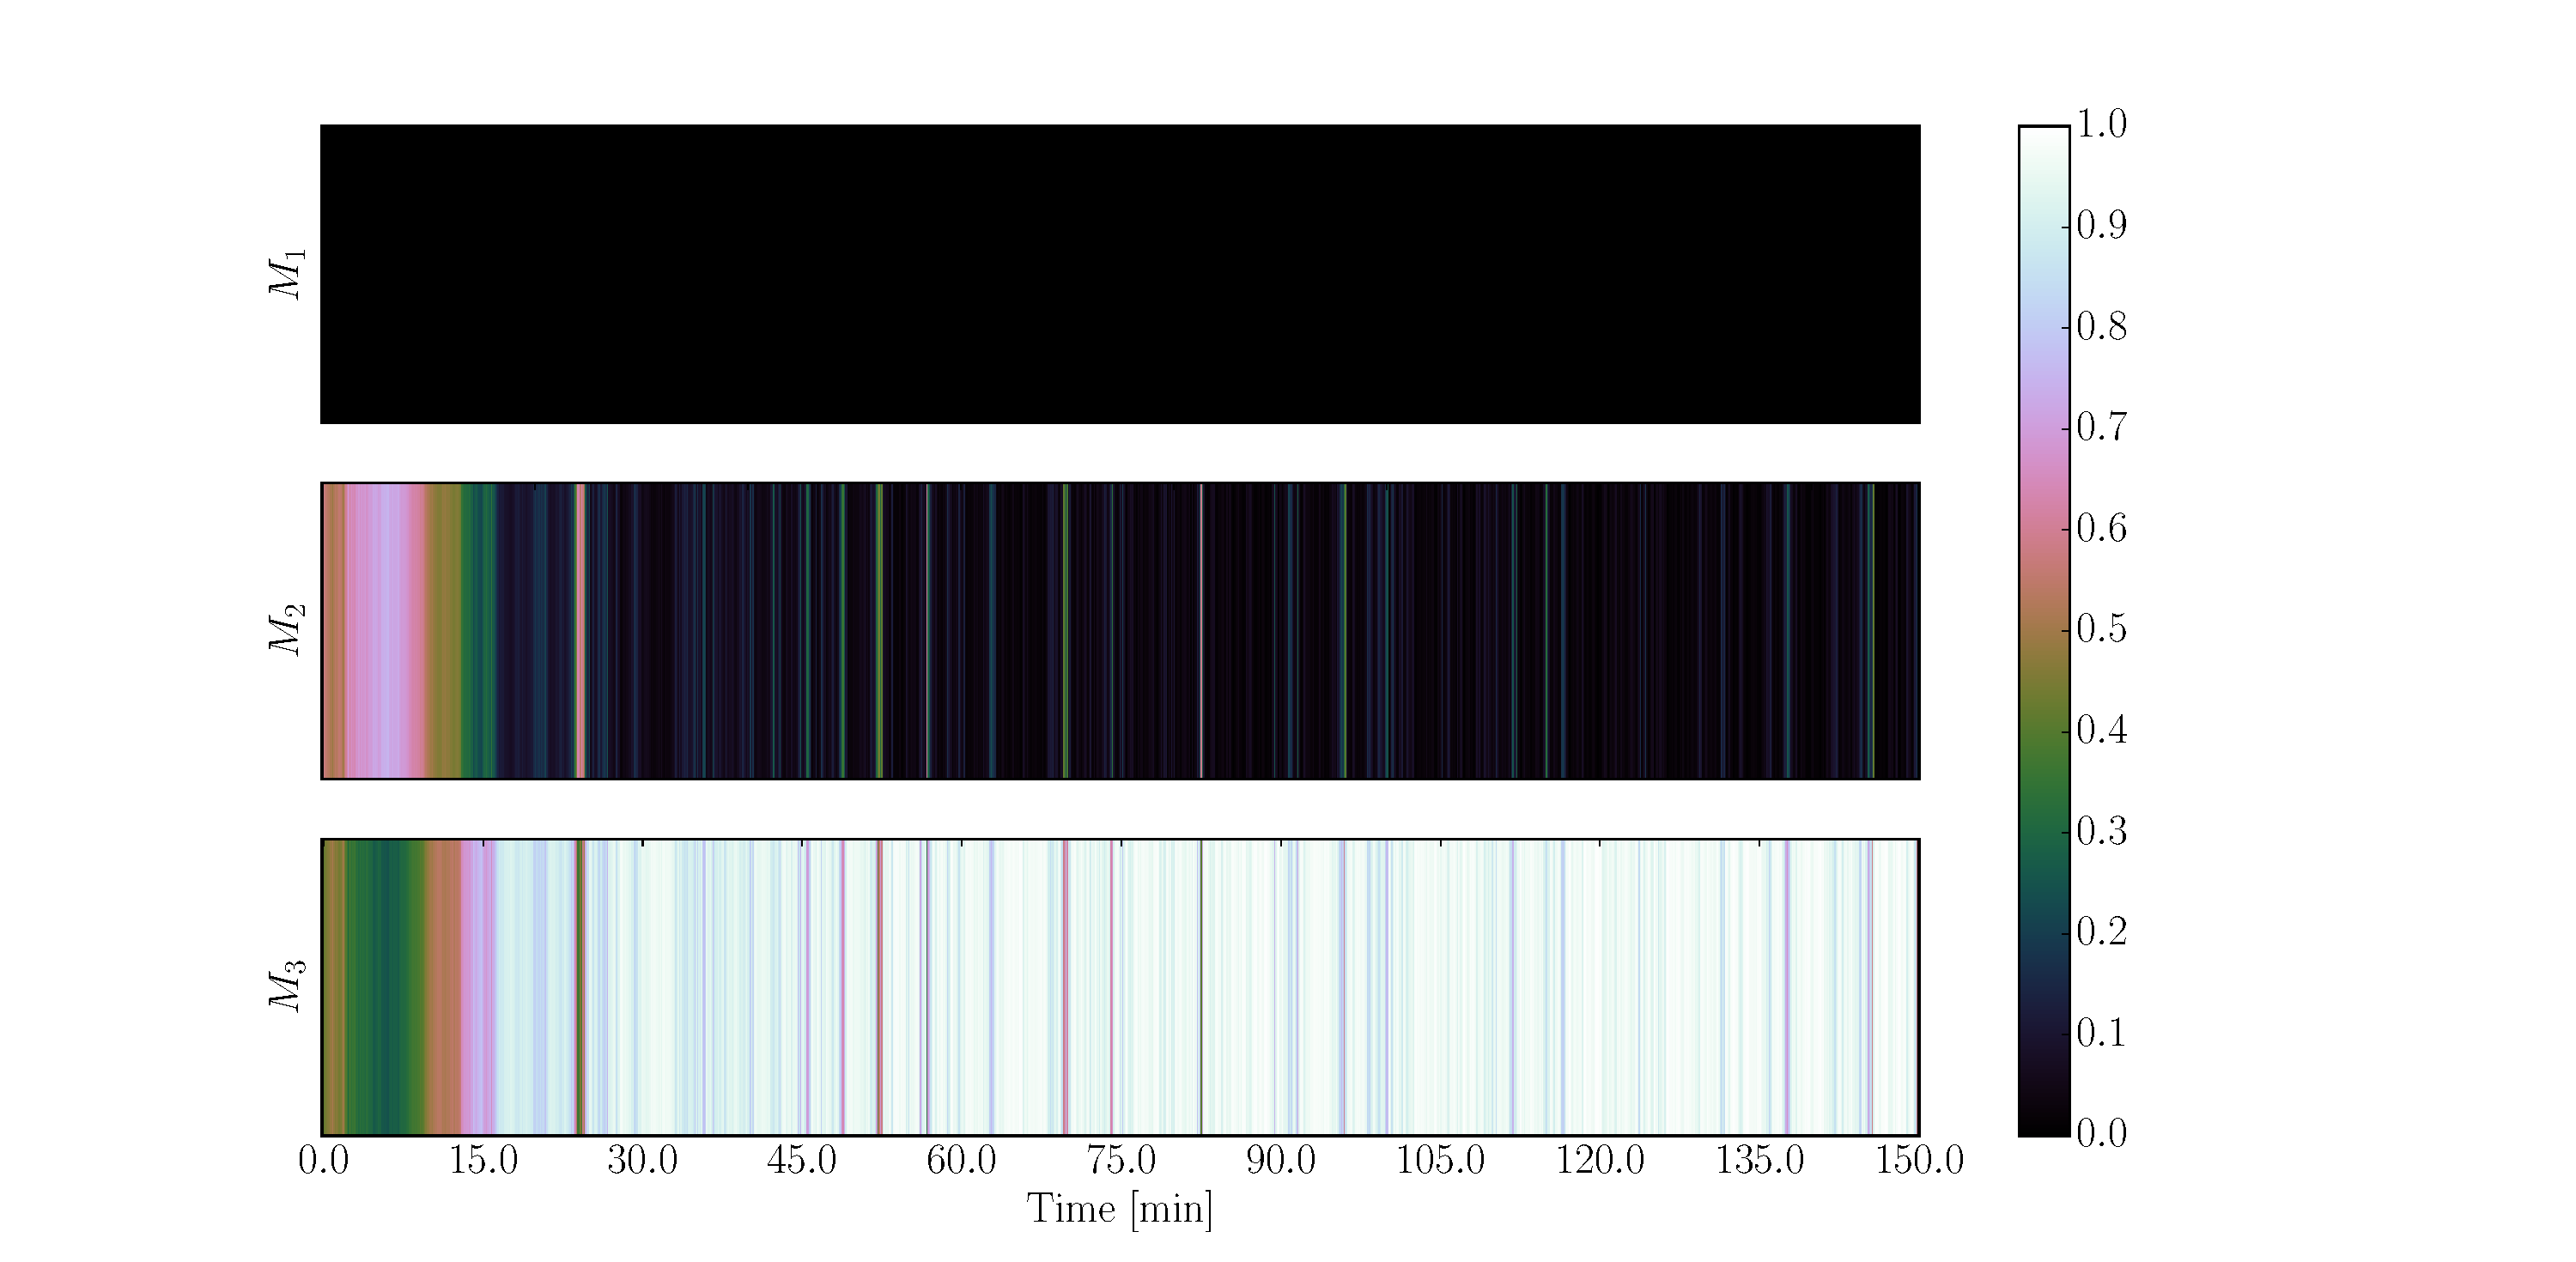
\includegraphics[scale=0.25]{rbpf_3m_switch_m2.pdf}
\caption{State of the switching variable $s_t$ over time. The weight indicates the sum of the particle weights per model.}
\label{fig_3m_switch_m2}
\end{figure}
Finally, in Figure \ref{fig_3m_maxswitch} we see only the most likely model at each time step. This is simply derived from Figure \ref{fig_3m_switch_m2} by selecting the particle with the highest weighted switching index.
\begin{figure}[H] 
\centering
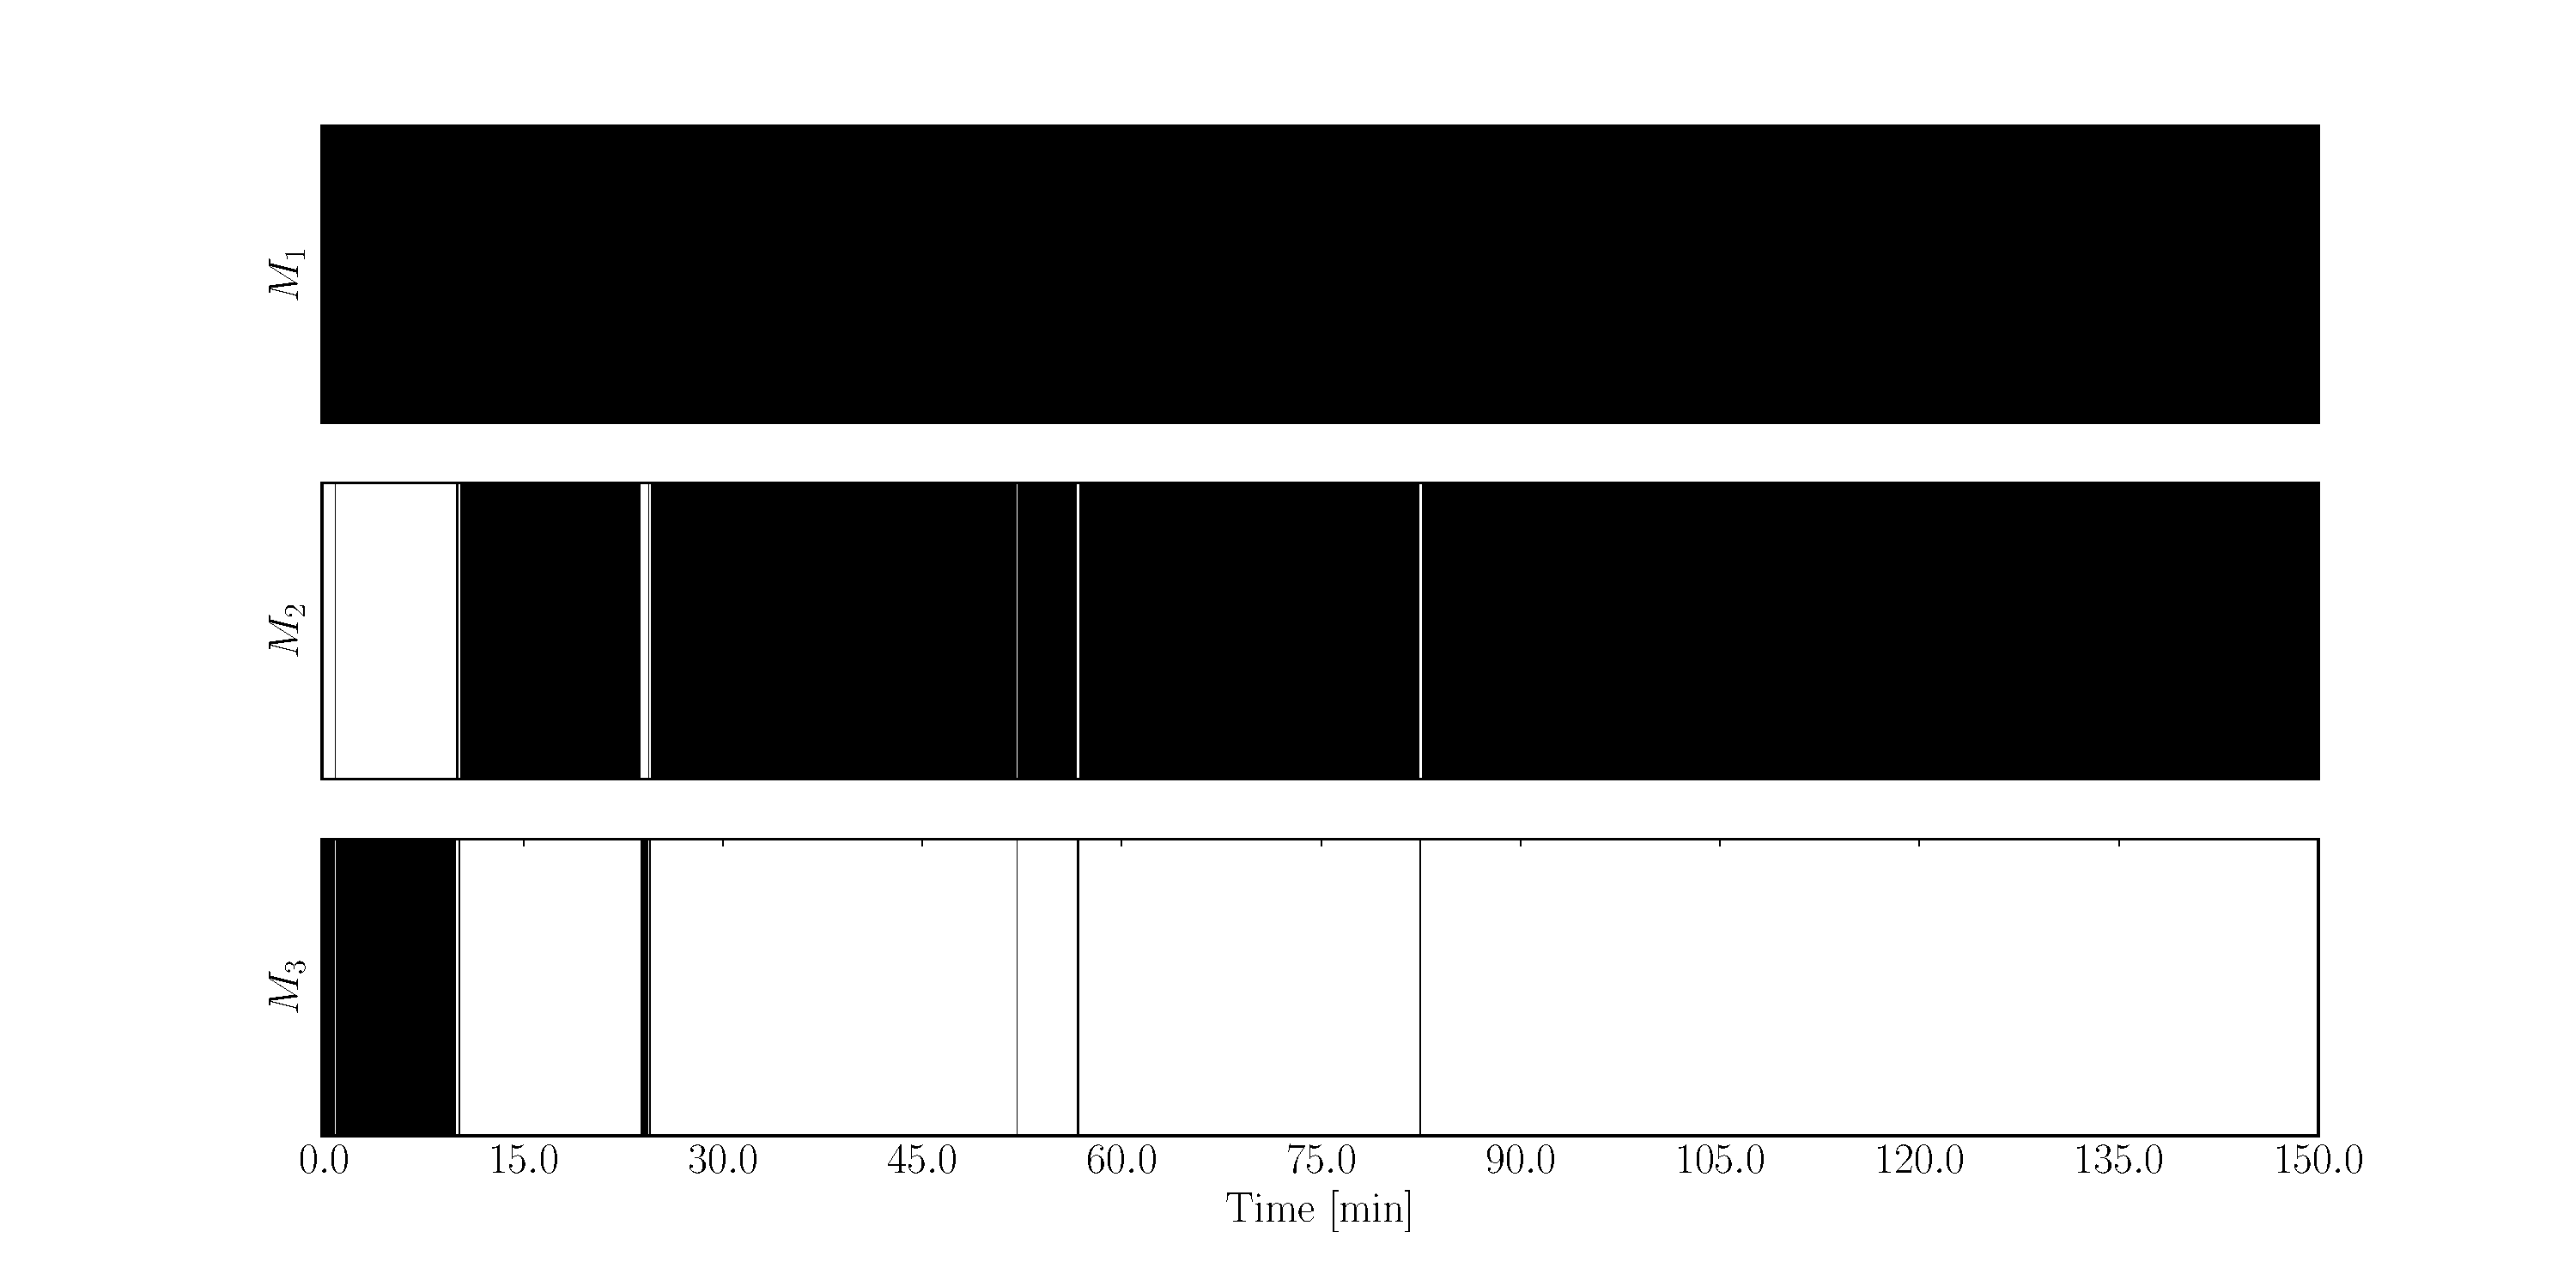
\includegraphics[scale=0.25]{rbpf_3m_maxswitch_m2.pdf}
\caption{State of the switching variable $s_t$ over time. The weight indicates the sum of the particle weights per model.}
\label{fig_3m_maxswitch}
\end{figure}
Since we only base our state estimate on the most likely particle Figure \ref{fig_3m_maxswitch} indicates from which model our state estimate is derived. Ideally one would like very little ``switching noise" i.e. as soon as the system moves into territory where $M_3$ is accurate no particles should have high $M_1$ or $M_2$ weight. We see that this is mostly the case in Figure \ref{fig_3m_maxswitch}. 
\chapter{Inference using nonlinear hybrid models}
\label{sec_inf_spf}
In this chapter we study the same graphical model as Chapter \ref{sec_inf_lin_hybrid}, shown in Figure \ref{fig_hybridmod2} for convenience, but we drop the assumption that the dynamic models used for inference are linear. The variables retain their meaning as before.     
\begin{figure}[H] 
\centering
\begin{tikzpicture}

  % Define nodes
  \node[obs] (ya) {$y_0$};
  \node[obs, right=of ya] (yb) {$y_1$};
  \node[obs, right=of yb] (yc) {$y_2$};
  \node[latent, above=of ya]  (xa) {$x_0$};
  \node[latent, above=of yb, right=of xa]  (xb) {$x_1$};
  \node[latent, above=of yc, right=of xb]  (xc) {$x_2$};
  \node[det, above=of xa, xshift=0.7cm] (da) {$u_0$};
  \node[det, above=of xb, xshift=0.7cm] (db) {$u_1$};
  \node[latent, above=of xa, yshift=1.1cm] (sa) {$s_0$};
  \node[latent, above=of xb, yshift=1.1cm] (sb) {$s_1$};
  \node[latent, above=of xc, yshift=1.1cm] (sc) {$s_2$};
  
  % Connect the nodes
  \edge {da} {xb};
  \edge {db} {xc};
  \edge {xa} {ya};
  \edge {xb} {yb};
  \edge {xc} {yc};
  \edge {xa} {xb};
  \edge {xb} {xc};
  \edge {sa} {sb};
  \edge {sb} {sc};
  \edge {sa} {xa};
  \edge {sb} {xb};
  \edge {sc} {xc};
  
\end{tikzpicture}
\caption{Graphical model of this chapter.}
\label{fig_hybridmod2}
\end{figure}
Intuitively we are now using the switching variables to decide which nonlinear model (or combination of) better describes the observed system behaviour. At each point in time we desire a weighted set of nonlinear models with the weight proportional to the ability of the model to explain the plant behaviour. Such a system could be used to describe significant model changes e.g. catalyst degradation in our CSTR or a reactor which breaks suddenly etc... 

We model this system as follows. Let $s_t$ denote a discrete $M$ state first order Markov chain with transition matrix $P$ as discussed in Chapter \ref{sec_inf_lin_hybrid}. Let each state $s_t=i$ be associated with a model set $\left(f_i, g_i, W_i, V_i \right)$ used to evaluate the dynamical model shown in (\ref{eq_smodel2}).
\begin{equation}
\begin{aligned}
x_{t+1} &= f_i(x_t, u_t, w_{t+1}) \text{ with } w_{t+1} \backsim \mathcal{N}(0, W_i)\\
y_{t+1} &= g_i(x_{t+1}, v_{t+1}) \text{ with } v_{t+1} \backsim \mathcal{N}(0,V_i)
\end{aligned}
\label{eq_smodel2}
\end{equation}
In this dissertation we assume that the the noise distributions are Gaussian but there is no fundamental reason why they cannot be arbitrary. To fully specify the system we again require the prior distributions $p(s_0)$ and $p(x_0|s_0)$ as well as the stochastic matrix $P$. In this chapter we manually specify the matrix $P$ but it can be computed using the Baum-Welch algorithm. 
\section{Exact filtering}
By extending the model to incorporate nonlinear models it becomes even more difficult to perform inference. It is clear that for the type of systems we consider here no exact inference algorithm, which is computationally feasible, exists \cite{murphy1}. We again turn to approximate inference algorithms.

Note that we cannot apply Rao-Blackwellisation (i.e. analytically evaluate the stochastic dynamical system component and approximate the switching component) as before because the dynamic models used for inference are no longer linear. We use the adaptive sequential importance resampling, i.e. the bootstrap particle filter, algorithm as discussed in Chapter \ref{sec_inf_nonlin_mods}.
\section{Switching particle filter}
We cannot analytically evaluate any part of the desired posterior distribution $p(s_{0:t}, x_{0:t}|y_{0:t})$ in a computationally feasible manner, so we must apply the adaptive sequential importance resampling algorithm to the entire state space of Figure \ref{fig_hybridmod2}. The algorithm follows straightforwardly from our discussion in Chapter \ref{sec_asir} \cite{murphy1}. We merely state the proposal distribution and incremental weight function we sample from in (\ref{eq_nonpf}). 
\begin{equation}
\begin{aligned}
&q_t(s_t,x_t|s_{0:t-1},x_{0:t-1,}y_{0:t}) = p(s_t|s_{t-1})p(x_t|s_t,x_{t-1}) \\
&\alpha_t(s_{0:t},x_{0:t}) = p(y_t|x_t,s_t)
\end{aligned}
\label{eq_nonpf}
\end{equation}  
Applying the algorithm is a straightforward extension of the bootstrap particle filter introduced in Chapter \ref{sec_bootstrap} given the weighting function and proposal distribution as shown below.

\textbf{Switching particle filter algorithm}\\
For $t=0$:
\begin{enumerate}
\item
Sample $S^i_0 \backsim p(s_0)$ and $X^i_0 \backsim p(x_0|s_0)$.
\item
Compute the weights $w_0(S_0^i, X_0^i) = p(y_0|S_0^i, X_0^i)$ where $y_0$ is the observation. Normalise $W^i_0 \propto w_0(S_0^i, X_0^i)$. 
\item
If the number of effective particles is below some threshold apply resampling with roughening $(W^i_0, S^i_0, X^i_0)$ to obtain $N$ equally weighted particles $(\frac{1}{N}, \bar{S}^i_0, \bar{X}^i_0)$ and set $(\bar{W}^i_0, \bar{S}^i_0,\bar{X}^i_0) \leftarrow (\frac{1}{N}, \bar{S}^i_0, \bar{X}^i_0)$ otherwise set $(\bar{W}^i_0,\bar{S}^i_0, \bar{X}^i_0) \leftarrow ({W}^i_0, S_0^i, {X}^i_0)$
\end{enumerate}
For $t \geq 1$:
\begin{enumerate}
\item
Sample $S^i_t \backsim p(S_t^i|\bar{S}^i_{t-1})$ and $X^i_t \backsim p(X^i_t|S^i_t, \bar{X}^i_{t-1})$.
\item
Compute the weights $\alpha_t(S_t^i, X_t^i) = p(y_t|S_t^i, X_t^i)$ where $y_t$ is the observation. Normalise $W^i_t \propto W^i_{t-1}\alpha_t(S_t^i, X_t^i)$.
\item
If the number of effective particles is below some threshold apply resampling with roughening $(W^i_t, S^i_t, X^i_t)$ to obtain $N$ equally weighted particles $(\frac{1}{N}, \bar{S}^i_t, \bar{X}^i_t)$ and set $(\bar{W}^i_t, \bar{S}^i_t,\bar{X}^i_t) \leftarrow (\frac{1}{N}, \bar{S}^i_t, \bar{X}^i_t)$ otherwise set $(\bar{W}^i_t,\bar{S}^i_t, \bar{X}^i_t) \leftarrow ({W}^i_t, S_t^i, {X}^i_t)$
\end{enumerate} 

\section{Switching particle prediction}
The prediction of the hybrid nonlinear states follows in an analogous manner to the prediction algorithm found in Chapter \ref{sec_particle_prediction}. We do not supply an algorithm because it is a straightforward simplification of the switching particle filter algorithm seen above: effectively there is no weight update step because there is no observation. The corresponding graphical model is shown in Figure \ref{fig_hybridmod2_prediction}.
\begin{figure}[H] 
\centering
\begin{tikzpicture}

  % Define nodes
  \node[obs] (ya) {$y_0$};
  \node[latent, above=of ya]  (xa) {$x_0$};
  \node[latent, above=of yb, right=of xa]  (xb) {$x_1$};
  \node[latent, above=of yc, right=of xb]  (xc) {$x_2$};
  \node[det, above=of xa, xshift=0.7cm] (da) {$u_0$};
  \node[det, above=of xb, xshift=0.7cm] (db) {$u_1$};
  \node[latent, above=of xa, yshift=1.1cm] (sa) {$s_0$};
  \node[latent, above=of xb, yshift=1.1cm] (sb) {$s_1$};
  \node[latent, above=of xc, yshift=1.1cm] (sc) {$s_2$};
  
  % Connect the nodes
  \edge {da} {xb};
  \edge {db} {xc};
  \edge {xa} {ya};
  \edge {xa} {xb};
  \edge {xb} {xc};
  \edge {sa} {sb};
  \edge {sb} {sc};
  \edge {sa} {xa};
  \edge {sb} {xb};
  \edge {sc} {xc};
  
\end{tikzpicture}
\caption{Switching particle prediction graphical model.}
\label{fig_hybridmod2_prediction}
\end{figure}  

\section{Smoothing and Viterbi decoding}
Like Chapter \ref{sec_inf_lin_hybrid} we refer the reader elsewhere for a detailed discussion on both smoothing and Viterbi decoding \cite{murphy1}. It suffices to say that given the nonlinear dynamics the aforementioned inference will be beyond the scope of this dissertation. 

\section{Filtering the CSTR}
\label{sec_spf_filtering}
In this chapter we illustrate the use of the switching particle filter using  two nonlinear dynamical model derived from the familiar CSTR example of Chapter \ref{sec_cstr}. Since the graphical model of Chapter \ref{sec_inf_lin_hybrid} is identical to that of Figure \ref{fig_hybridmod2} we expect that the general trends discussed in Chapter \ref{sec_rbpf_filtering_cstr} to hold here as well.

For the purposes of illustration we assume a scenario where the rate constant of the CSTR decreases by an order of magnitude. This scenario is not completely arbitrary, for example, this could be caused by catalyst degradation due to some environmental factor. It is our aim to infer when this happens and to be able to track the states accurately despite the significant model change. Therefore we will have one nonlinear model of the healthy plant $M_1$ and one nonlinear model of the faulty plant $M_2$.

Note that the character of the inference we are attempting to do is fundamentally different from that of Chapter \ref{sec_inf_lin_hybrid} but that the underlying graphical models are the same. In Chapter \ref{sec_inf_lin_hybrid} the Rao-Blackwellised particle filter switched between models which all attempt to describe the same physical system albeit in different regions of the state space. In this chapter the switching particle filter will attempt to switch between models which describe completely different physical systems. This difference informs our choice of the switch transition matrix.

We use 500 particles during all runs for the switching particle filter and use the switching transition matrix $P_1=\begin{pmatrix}
0.99 & 0.01 \\ 0.01 & 0.99
\end{pmatrix}$. For the particle filter, used for a comparative base, we use 200 particles. We spent much time in Chapter \ref{sec_rbpf_filtering_cstr} discussing the effect the switch transition matrix has on model selection. The form of the matrix is motivated by physical considerations as well: once the catalyst denatures it is unlikely to fix itself. Thus, once the model breaks, switches from $M_1$ to $M_2$, it is unlikely to switch back. In all the simulations the catalyst denatures at 50 minutes into the run.

We conduct two brief, but illustrative, investigations comparing the effectiveness of the switching particle filter and the particle filter. In both cases the particle filter uses the healthy system model - the benefit of the additional complexity of the switching particle filter model is to be highlighted here. In the first investigation we measure only temperature and in the second we measure both concentration and temperature. 

In Figure \ref{fig_pf_m1_compspf} we illustrate the tracking performance\footnote{Unfortunately we cannot use the average tracking performance measures used previously. Since the filter approaches a concentration of 0 $\text{kmol.m}^{-3}$ the average error estimates are not accurate: there is division by very small numbers. We thus rely on a visual comparison.} of the particle filter on the system. Note that the simulation window is very long - 600 minutes.
\begin{figure}[H] 
\centering
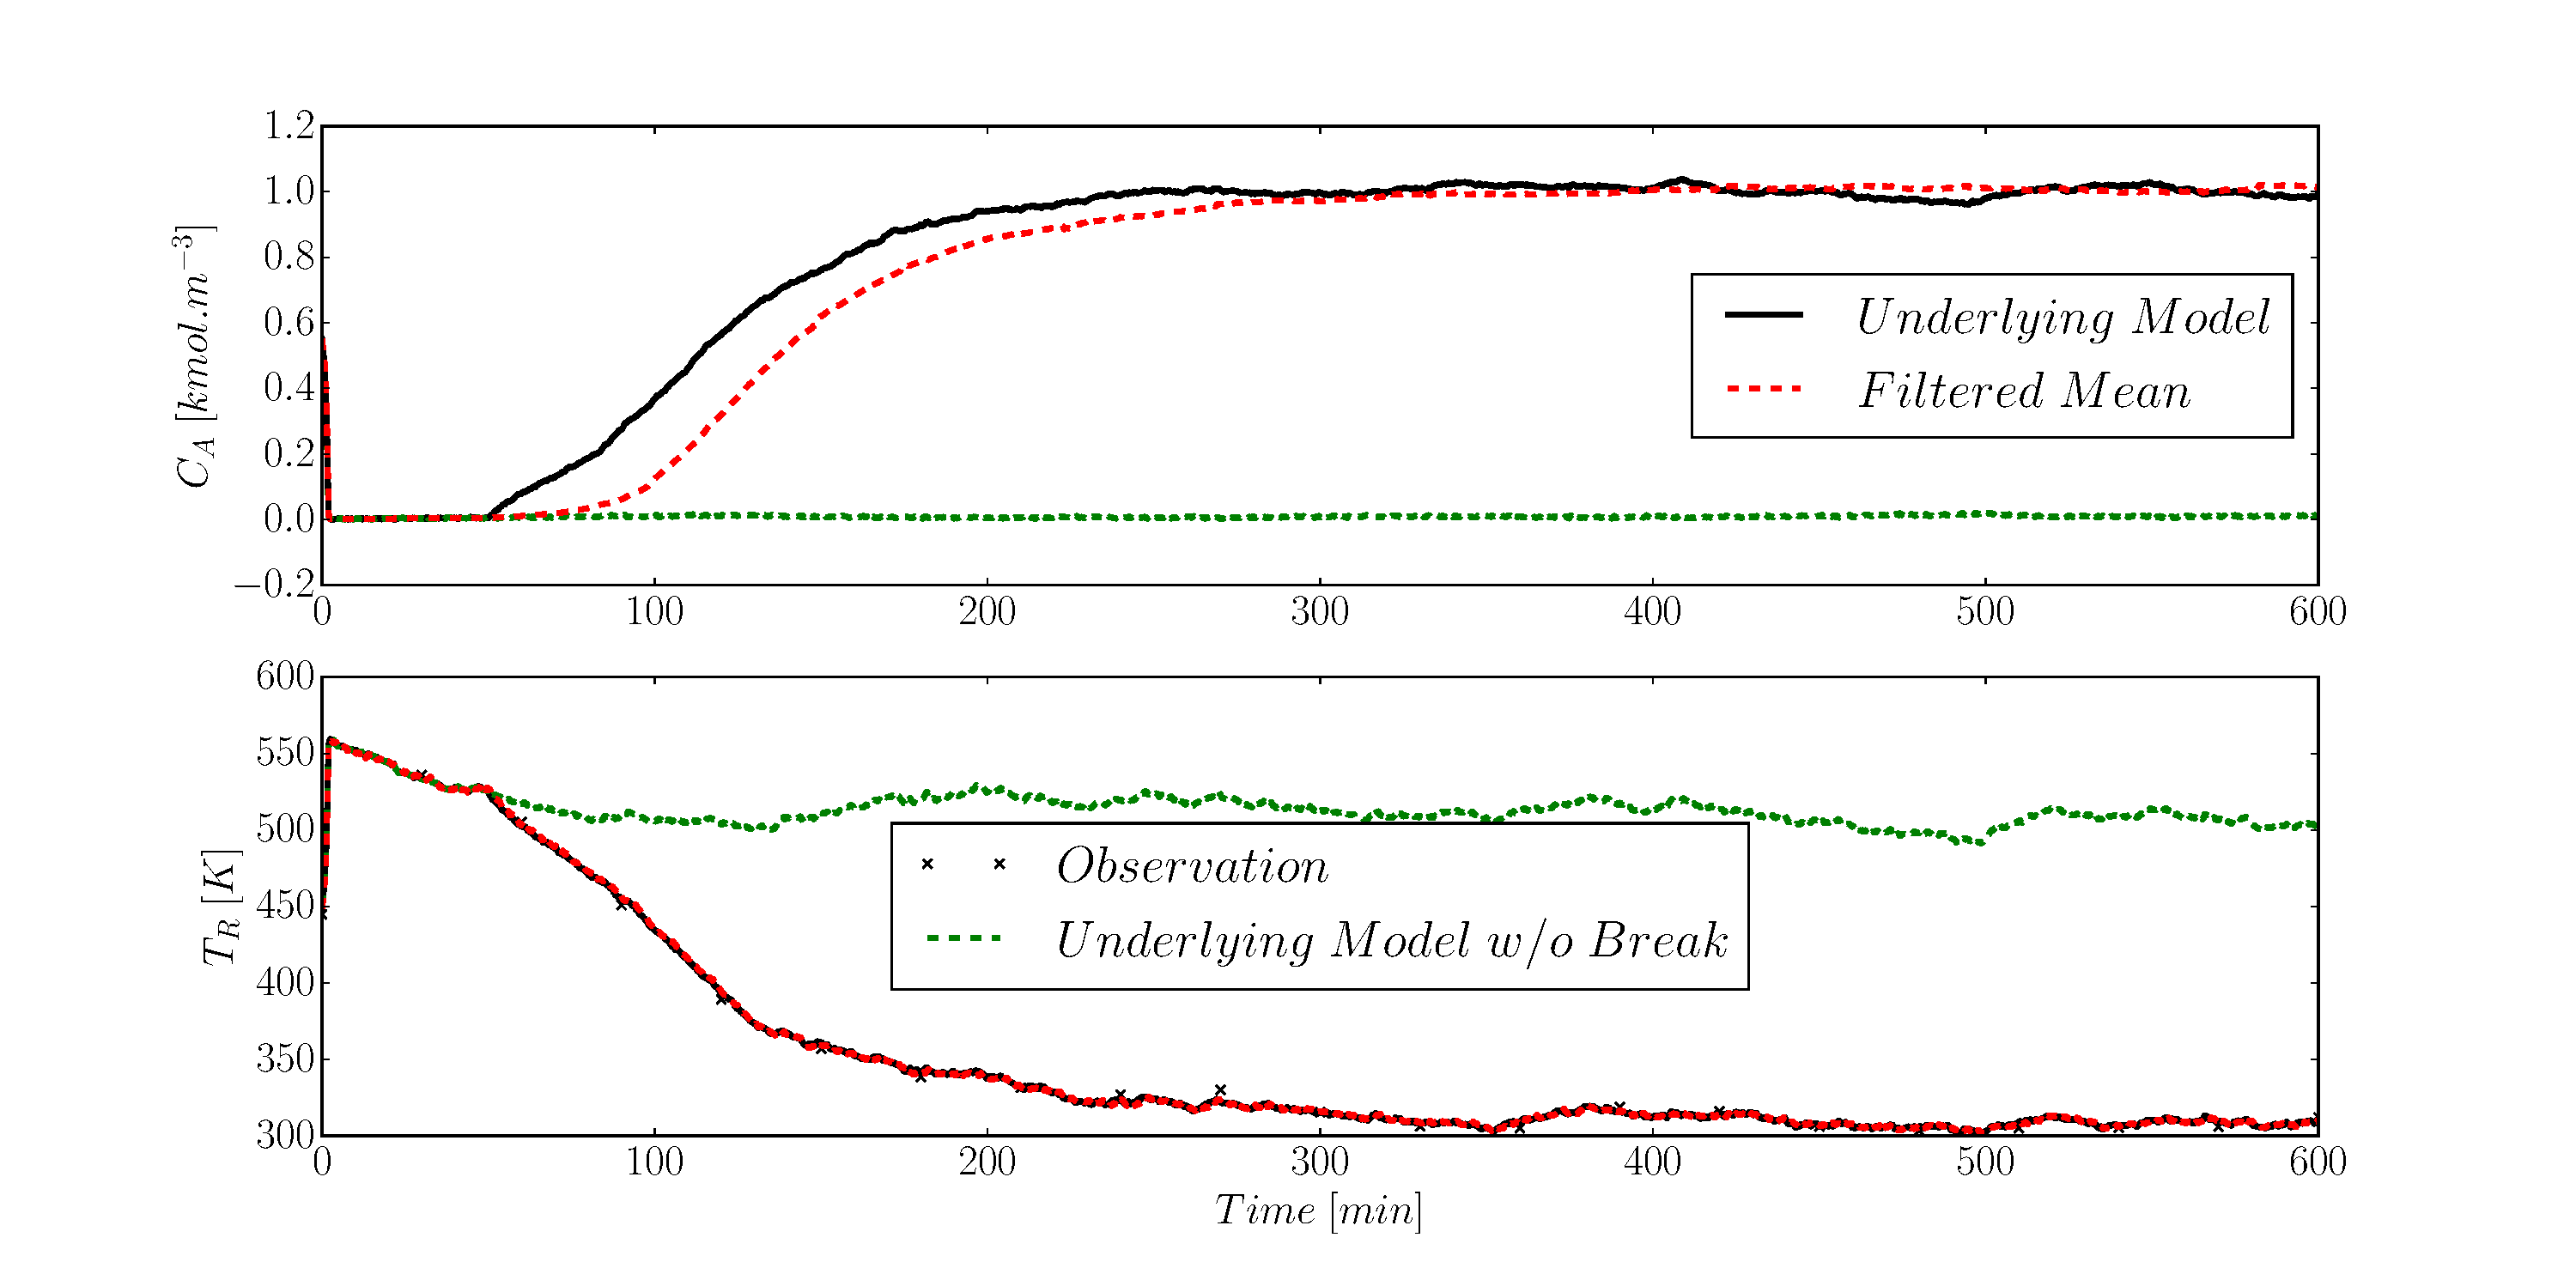
\includegraphics[width=\textwidth]{pf_m1_compspf.pdf}
\caption{Particle filter using 200 particles tracking the CSTR where the catalyst denatures at 50 minutes. Only temperature is measured.}
\label{fig_pf_m1_compspf}
\end{figure}
It is clear that the particle filter tracks the temperature well, because it is measured, but tracks the concentration very poorly. It takes almost 300 minutes before the particle filter estimates the concentration reliably. Clearly the model mismatch causes the filter's poor performance - compare this to the excellent tracking in Chapter \ref{sec_nonlinmods_filtering}.

In Figure \ref{fig_spf_m1_track} we see the tracking performance of the switching particle filter measuring only temperature.
\begin{figure}[H] 
\centering
\includegraphics[width=\textwidth]{spf_m1_track.pdf}
\caption{switching particle filter using 500 particles tracking the CSTR where the catalyst denatures at 50 minutes.}
\label{fig_spf_m1_track}
\end{figure}
It is clear that the switching particle filter tracks the states very well. However, Figure \ref{fig_spf_m1_switch} indicates that we have the some switching noise problems.
\begin{figure}[H] 
\centering
\includegraphics[width=\textwidth]{spf_m1_switch.pdf}
\caption{Switching particle filter measuring only temperature. The switching weight of each particle is shown per time step. $M_1$ corresponds to the healthy plant and $M_2$ to the broken plant.}
\label{fig_spf_m1_switch}
\end{figure} 
It is not surprising that there is switching noise: the graphical models of this and Chapter \ref{sec_inf_lin_hybrid} are the same. However, we do see that the switching particle filter switches models at about 50 minutes. This indicates that the filter effectively identifies when the process fault occurs. It seems that after the fault has been identified there is a period where the filter reliably isolates the correct underlying model thereafter, from about 130 minutes, both models are equally likely. It seems there is a regime near the unstable operating point where the models are maximally different. Conversely, near the low temperature operating point (near the end of the simulation) the models are quite similar. This is physically believable because both those operating points correspond to a system where almost no conversion occurs; therefore broken or not the models would generate the similar predictions. Therefore, switching noise caused by model overlap is only a problem in this region.

Figure \ref{fig_pf_m2_compspf} illustrates the filtering performance of the particle filter using both state measurements.
\begin{figure}[H] 
\centering
\includegraphics[width=\textwidth]{pf_m2_compspf.pdf}
\caption{Particle filter using 200 particles tracking the CSTR where the catalyst denatures at 50 minutes. Both states are measured.}
\label{fig_pf_m2_compspf}
\end{figure}
Clearly measuring both states is beneficial in terms of filter performance. The state estimation deviation seen in Figure \ref{fig_pf_m1_compspf} is significantly less here - by approximately 150 minutes the particle filter is tracking the underlying system.

Figure \ref{fig_spf_m2_track} shows the filtering performance of the switching particle filter. 
\begin{figure}[H] 
\centering
\includegraphics[width=\textwidth]{spf_m2_track.pdf}
\caption{Switching particle filter using 500 particles tracking the CSTR where the catalyst denatures at 50 minutes. Both states are measured.}
\label{fig_spf_m2_track}
\end{figure}
Again the performance is very good - the filter accurately tracks the underlying states. In Figure \ref{fig_spf_m2_switch} there is significantly less switching noise in the first 100 minutes of the simulation than in Figure \ref{fig_spf_m1_switch}.
\begin{figure}[H] 
\centering
\includegraphics[width=\textwidth]{spf_m2_switch.pdf}
\caption{Switching particle filter measuring both concentration and temperature. The switching weight of each particle is shown per time step.}
\label{fig_spf_m2_switch}
\end{figure} 
It is clear that the second measurement helps the filter differentiate between the regimes of the healthy and broken plant when the system is near the high temperature and unstable operating points. However, we see the same behaviour near the low temperature operating point - the models are clearly similar here and we again have the problem of model overlap. 

In the next chapter we implement control using the switching particle filter to identify when the underlying system's dynamics have changed. 

\section{Stochastic Switching Linear Control}

\subsection{Current Literature}

\subsection{Unconstrained Control}

\subsection{Constrained Control}


\chapter{Future Work}

\section{Parameter Optimisation}
Parameter optimisation for objective functions

\section{Augmented Switching Graphical Model}
Graphical model extension ASKF

\section{Stochastic Inputs Graphical Model}
Stochastic inputs like PDV

\chapter{Conclusion}
To do.


%References
\newpage
\bibliographystyle{plain}
\bibliography{./docs/research}

\end{document}